\documentclass[]{book}
\usepackage{lmodern}
\usepackage{amssymb,amsmath}
\usepackage{ifxetex,ifluatex}
\usepackage{fixltx2e} % provides \textsubscript
\ifnum 0\ifxetex 1\fi\ifluatex 1\fi=0 % if pdftex
  \usepackage[T1]{fontenc}
  \usepackage[utf8]{inputenc}
\else % if luatex or xelatex
  \ifxetex
    \usepackage{mathspec}
  \else
    \usepackage{fontspec}
  \fi
  \defaultfontfeatures{Ligatures=TeX,Scale=MatchLowercase}
\fi
% use upquote if available, for straight quotes in verbatim environments
\IfFileExists{upquote.sty}{\usepackage{upquote}}{}
% use microtype if available
\IfFileExists{microtype.sty}{%
\usepackage{microtype}
\UseMicrotypeSet[protrusion]{basicmath} % disable protrusion for tt fonts
}{}
\usepackage{hyperref}
\hypersetup{unicode=true,
            pdftitle={R Scripts for Longitudinal and Panel Data},
            pdfauthor={Yumo Dong, Edward Frees, and others??},
            pdfborder={0 0 0},
            breaklinks=true}
\urlstyle{same}  % don't use monospace font for urls
\usepackage{natbib}
\bibliographystyle{econPeriod}
\usepackage{color}
\usepackage{fancyvrb}
\newcommand{\VerbBar}{|}
\newcommand{\VERB}{\Verb[commandchars=\\\{\}]}
\DefineVerbatimEnvironment{Highlighting}{Verbatim}{commandchars=\\\{\}}
% Add ',fontsize=\small' for more characters per line
\usepackage{framed}
\definecolor{shadecolor}{RGB}{248,248,248}
\newenvironment{Shaded}{\begin{snugshade}}{\end{snugshade}}
\newcommand{\AlertTok}[1]{\textcolor[rgb]{0.94,0.16,0.16}{#1}}
\newcommand{\AnnotationTok}[1]{\textcolor[rgb]{0.56,0.35,0.01}{\textbf{\textit{#1}}}}
\newcommand{\AttributeTok}[1]{\textcolor[rgb]{0.77,0.63,0.00}{#1}}
\newcommand{\BaseNTok}[1]{\textcolor[rgb]{0.00,0.00,0.81}{#1}}
\newcommand{\BuiltInTok}[1]{#1}
\newcommand{\CharTok}[1]{\textcolor[rgb]{0.31,0.60,0.02}{#1}}
\newcommand{\CommentTok}[1]{\textcolor[rgb]{0.56,0.35,0.01}{\textit{#1}}}
\newcommand{\CommentVarTok}[1]{\textcolor[rgb]{0.56,0.35,0.01}{\textbf{\textit{#1}}}}
\newcommand{\ConstantTok}[1]{\textcolor[rgb]{0.00,0.00,0.00}{#1}}
\newcommand{\ControlFlowTok}[1]{\textcolor[rgb]{0.13,0.29,0.53}{\textbf{#1}}}
\newcommand{\DataTypeTok}[1]{\textcolor[rgb]{0.13,0.29,0.53}{#1}}
\newcommand{\DecValTok}[1]{\textcolor[rgb]{0.00,0.00,0.81}{#1}}
\newcommand{\DocumentationTok}[1]{\textcolor[rgb]{0.56,0.35,0.01}{\textbf{\textit{#1}}}}
\newcommand{\ErrorTok}[1]{\textcolor[rgb]{0.64,0.00,0.00}{\textbf{#1}}}
\newcommand{\ExtensionTok}[1]{#1}
\newcommand{\FloatTok}[1]{\textcolor[rgb]{0.00,0.00,0.81}{#1}}
\newcommand{\FunctionTok}[1]{\textcolor[rgb]{0.00,0.00,0.00}{#1}}
\newcommand{\ImportTok}[1]{#1}
\newcommand{\InformationTok}[1]{\textcolor[rgb]{0.56,0.35,0.01}{\textbf{\textit{#1}}}}
\newcommand{\KeywordTok}[1]{\textcolor[rgb]{0.13,0.29,0.53}{\textbf{#1}}}
\newcommand{\NormalTok}[1]{#1}
\newcommand{\OperatorTok}[1]{\textcolor[rgb]{0.81,0.36,0.00}{\textbf{#1}}}
\newcommand{\OtherTok}[1]{\textcolor[rgb]{0.56,0.35,0.01}{#1}}
\newcommand{\PreprocessorTok}[1]{\textcolor[rgb]{0.56,0.35,0.01}{\textit{#1}}}
\newcommand{\RegionMarkerTok}[1]{#1}
\newcommand{\SpecialCharTok}[1]{\textcolor[rgb]{0.00,0.00,0.00}{#1}}
\newcommand{\SpecialStringTok}[1]{\textcolor[rgb]{0.31,0.60,0.02}{#1}}
\newcommand{\StringTok}[1]{\textcolor[rgb]{0.31,0.60,0.02}{#1}}
\newcommand{\VariableTok}[1]{\textcolor[rgb]{0.00,0.00,0.00}{#1}}
\newcommand{\VerbatimStringTok}[1]{\textcolor[rgb]{0.31,0.60,0.02}{#1}}
\newcommand{\WarningTok}[1]{\textcolor[rgb]{0.56,0.35,0.01}{\textbf{\textit{#1}}}}
\usepackage{longtable,booktabs}
\usepackage{graphicx,grffile}
\makeatletter
\def\maxwidth{\ifdim\Gin@nat@width>\linewidth\linewidth\else\Gin@nat@width\fi}
\def\maxheight{\ifdim\Gin@nat@height>\textheight\textheight\else\Gin@nat@height\fi}
\makeatother
% Scale images if necessary, so that they will not overflow the page
% margins by default, and it is still possible to overwrite the defaults
% using explicit options in \includegraphics[width, height, ...]{}
\setkeys{Gin}{width=\maxwidth,height=\maxheight,keepaspectratio}
\IfFileExists{parskip.sty}{%
\usepackage{parskip}
}{% else
\setlength{\parindent}{0pt}
\setlength{\parskip}{6pt plus 2pt minus 1pt}
}
\setlength{\emergencystretch}{3em}  % prevent overfull lines
\providecommand{\tightlist}{%
  \setlength{\itemsep}{0pt}\setlength{\parskip}{0pt}}
\setcounter{secnumdepth}{5}
% Redefines (sub)paragraphs to behave more like sections
\ifx\paragraph\undefined\else
\let\oldparagraph\paragraph
\renewcommand{\paragraph}[1]{\oldparagraph{#1}\mbox{}}
\fi
\ifx\subparagraph\undefined\else
\let\oldsubparagraph\subparagraph
\renewcommand{\subparagraph}[1]{\oldsubparagraph{#1}\mbox{}}
\fi

%%% Use protect on footnotes to avoid problems with footnotes in titles
\let\rmarkdownfootnote\footnote%
\def\footnote{\protect\rmarkdownfootnote}

%%% Change title format to be more compact
\usepackage{titling}

% Create subtitle command for use in maketitle
\providecommand{\subtitle}[1]{
  \posttitle{
    \begin{center}\large#1\end{center}
    }
}

\setlength{\droptitle}{-2em}

  \title{R Scripts for Longitudinal and Panel Data}
    \pretitle{\vspace{\droptitle}\centering\huge}
  \posttitle{\par}
    \author{Yumo Dong, Edward Frees, and others??}
    \preauthor{\centering\large\emph}
  \postauthor{\par}
    \date{}
    \predate{}\postdate{}
  
\usepackage{booktabs}
\setcounter{secnumdepth}{2}

\begin{document}
\maketitle

{
\setcounter{tocdepth}{2}
\tableofcontents
}
\hypertarget{preface}{%
\chapter*{Preface}\label{preface}}
\addcontentsline{toc}{chapter}{Preface}

\emph{Date: 14 September 2019}

Here are \texttt{R} scripts for the book \textbf{Longitudinal and Panel Data} by Edward W. Frees. See the \href{https://instruction.bus.wisc.edu/jfrees/jfreesbooks/Longitudinal\%20and\%20Panel\%20Data/Book/PDataBook.htm}{book web site}.

The \href{https://instruction.bus.wisc.edu/jfrees/jfreesbooks/Longitudinal\%20and\%20Panel\%20Data/Book/DataFiles.htm}{datasets} may be downloaded from downloaded from website.

We will review these scripts in our \href{https://sites.google.com/a/wisc.edu/copula-study-group/}{Panel and Copula Reading Group}.

As a group, it may be worth our time to update and polish these scripts. They were first done in 2003 and have not received a lot of cleansing since that time. If you contribute, then this will help polish your \texttt{R} skills, as well as learn a bit about \texttt{Github}, where the scripts and this output is being hosted. For more on actuarial education on the web through \texttt{Github}, see the \href{https://ewfrees.github.io/}{Open Actuarial Textbooks} project.

\hypertarget{introduction}{%
\chapter{Introduction}\label{introduction}}

\hypertarget{import-data}{%
\section{Import Data}\label{import-data}}

First, we can import ``Divorce.txt'' downloaded from website \url{https://instruction.bus.wisc.edu/jfrees/jfreesbooks/Longitudinal\%20and\%20Panel\%20Data/Book/DataFiles.htm}

These are data describing the divorce rate in each state. In addition, there is other socioeconomic information about a state that may be related to the divorce rate. In particular, data concerning the number of marriages and births, unemployment and crime rates, and AFDC (Aid to Families with Dependent Children) payments are available. In this file, data are available for the years 1965, 1975, 1985 and 1995. The information provided by this study is potentially useful for governing agencies in budgeting for social needs such as judicial and welfare services that are affected by divorce. The data for the study were collected from various U.S. Statistical Abstracts. Divorce rate is defined as the number of divorces and annulments per thousand population per state. The independent variables include the number of marriages and live births per thousand population, the total unemployment rate as percent of total work force, the average monthly AFDC payments per family, and the total number of criminal offenses known to the police (murder, rape, robbery, aggravated assault, burglary, larceny, and motor vehicle theft). Some of the data points contain missing observations due to unavailability, and Nevada is unusual due to its uniquely high and unrepresentative marriage and divorce rates. Source: U.S. Statistical Abstract, various issues.

\begin{longtable}[]{@{}ll@{}}
\toprule
\begin{minipage}[b]{0.06\columnwidth}\raggedright
Variable\strut
\end{minipage} & \begin{minipage}[b]{0.88\columnwidth}\raggedright
Description\strut
\end{minipage}\tabularnewline
\midrule
\endhead
\begin{minipage}[t]{0.06\columnwidth}\raggedright
DIVORCE\strut
\end{minipage} & \begin{minipage}[t]{0.88\columnwidth}\raggedright
Number of divorces and annulments per state per one thousand population.\strut
\end{minipage}\tabularnewline
\begin{minipage}[t]{0.06\columnwidth}\raggedright
BIRTH\strut
\end{minipage} & \begin{minipage}[t]{0.88\columnwidth}\raggedright
Number of live births per state per one thousand population.\strut
\end{minipage}\tabularnewline
\begin{minipage}[t]{0.06\columnwidth}\raggedright
MARRIAGE\strut
\end{minipage} & \begin{minipage}[t]{0.88\columnwidth}\raggedright
Number of marriages per state per one thousand population.\strut
\end{minipage}\tabularnewline
\begin{minipage}[t]{0.06\columnwidth}\raggedright
UNEMPLOY\strut
\end{minipage} & \begin{minipage}[t]{0.88\columnwidth}\raggedright
Total unemployment rate as a percentage of the total work force.\strut
\end{minipage}\tabularnewline
\begin{minipage}[t]{0.06\columnwidth}\raggedright
CRIME\strut
\end{minipage} & \begin{minipage}[t]{0.88\columnwidth}\raggedright
Total number of criminal offenses (murder, rape, robbery, aggravated assault, burglary, larceny and motor vehicle theft) known to police per one hundred thousand population.\strut
\end{minipage}\tabularnewline
\begin{minipage}[t]{0.06\columnwidth}\raggedright
AFDC\strut
\end{minipage} & \begin{minipage}[t]{0.88\columnwidth}\raggedright
Average monthly AFDC (Aid to Families with Dependent Children) payments per family.\strut
\end{minipage}\tabularnewline
\begin{minipage}[t]{0.06\columnwidth}\raggedright
STATE\strut
\end{minipage} & \begin{minipage}[t]{0.88\columnwidth}\raggedright
State identifier, 1-51.\strut
\end{minipage}\tabularnewline
\begin{minipage}[t]{0.06\columnwidth}\raggedright
TIME\strut
\end{minipage} & \begin{minipage}[t]{0.88\columnwidth}\raggedright
Time identifier, 1-4.\strut
\end{minipage}\tabularnewline
\bottomrule
\end{longtable}

\begin{Shaded}
\begin{Highlighting}[]
\CommentTok{#  "\textbackslash{}t"  INDICATES SEPARATED BY TABLES  ;}
\NormalTok{divorce =}\StringTok{ }\KeywordTok{read.table}\NormalTok{(}\StringTok{"TXTData/Divorce.txt"}\NormalTok{, }\DataTypeTok{sep =}\StringTok{"}\CharTok{\textbackslash{}t}\StringTok{"}\NormalTok{, }\DataTypeTok{quote =} \StringTok{""}\NormalTok{,}\DataTypeTok{header=}\OtherTok{TRUE}\NormalTok{)}
\CommentTok{# divorce = read.table(choose.files(), sep ="\textbackslash{}t", quote = "",header=TRUE)}
\end{Highlighting}
\end{Shaded}

Let's have a look at the dataset. The names of variables and the first 8 rows observations.

\begin{Shaded}
\begin{Highlighting}[]
\CommentTok{#  PROVIDES THE NAMES IN THE FILE AND LISTS THE FIRST 8 OBSERVATIONS  ;}
\KeywordTok{names}\NormalTok{ (divorce)}
\end{Highlighting}
\end{Shaded}

\begin{verbatim}
 [1] "DIVORCE"    "BIRTH"      "MARRIAGE"   "UNEMPLOY"   "CRIME"     
 [6] "AFDC"       "STATE"      "TIME"       "STATE.Name" "Region"    
\end{verbatim}

\begin{Shaded}
\begin{Highlighting}[]
\NormalTok{divorce[}\DecValTok{1}\OperatorTok{:}\DecValTok{8}\NormalTok{,]}
\end{Highlighting}
\end{Shaded}

\begin{verbatim}
  DIVORCE BIRTH MARRIAGE UNEMPLOY  CRIME AFDC STATE TIME    STATE.Name
1     2.6  19.9      8.8      4.9  6.799  114     1    1         Maine
2     2.3  19.5     13.4      2.8  6.106  188     2    1 New Hampshire
3     1.5  20.5      9.0      4.2  5.793  113     3    1       Vermont
4     1.5  18.8      7.1      4.9 15.072  188     4    1 Massachusetts
5     1.3  19.4      7.1      4.9 14.180  172     5    1  Rhode Island
6     1.3  19.2      7.4      3.9 11.749  197     6    1   Connecticut
7     0.5  18.6      7.4      4.6 22.509  218     7    1      New York
8     0.8  18.5      6.8      5.1 13.966  203     8    1    New Jersey
           Region
1     New England
2     New England
3     New England
4     New England
5     New England
6     New England
7 Middle Atlantic
8 Middle Atlantic
\end{verbatim}

We can check some summary statistics. The dimension of \texttt{divorce}.

\begin{Shaded}
\begin{Highlighting}[]
\CommentTok{#  SUMMARY STATISTICS  ;}
\KeywordTok{dim}\NormalTok{(divorce)}
\end{Highlighting}
\end{Shaded}

\begin{verbatim}
[1] 204  10
\end{verbatim}

A summary of variables \texttt{DIVORCE} and \texttt{AFDC}.

\begin{Shaded}
\begin{Highlighting}[]
\KeywordTok{summary}\NormalTok{(divorce[, }\KeywordTok{c}\NormalTok{(}\StringTok{"DIVORCE"}\NormalTok{, }\StringTok{"AFDC"}\NormalTok{)])}
\end{Highlighting}
\end{Shaded}

\begin{verbatim}
    DIVORCE           AFDC      
 Min.   :0.500   Min.   : 33.0  
 1st Qu.:3.300   1st Qu.:154.0  
 Median :4.250   Median :224.0  
 Mean   :4.361   Mean   :245.9  
 3rd Qu.:5.300   3rd Qu.:315.0  
 Max.   :9.100   Max.   :731.0  
 NA's   :12      NA's   :3      
\end{verbatim}

\begin{Shaded}
\begin{Highlighting}[]
\KeywordTok{sd}\NormalTok{(divorce[,}\KeywordTok{c}\NormalTok{(}\StringTok{"DIVORCE"}\NormalTok{)], }\DataTypeTok{na.rm=}\OtherTok{TRUE}\NormalTok{) }\CommentTok{#The standard deviation of DIVORCE.}
\end{Highlighting}
\end{Shaded}

\begin{verbatim}
[1] 1.704068
\end{verbatim}

\begin{Shaded}
\begin{Highlighting}[]
\KeywordTok{sd}\NormalTok{(divorce[,}\KeywordTok{c}\NormalTok{(}\StringTok{"AFDC"}\NormalTok{)], }\DataTypeTok{na.rm=}\OtherTok{TRUE}\NormalTok{) }\CommentTok{#The standard deviation of AFDC.}
\end{Highlighting}
\end{Shaded}

\begin{verbatim}
[1] 122.2453
\end{verbatim}

\begin{Shaded}
\begin{Highlighting}[]
\KeywordTok{cor}\NormalTok{(divorce}\OperatorTok{$}\NormalTok{DIVORCE, divorce}\OperatorTok{$}\NormalTok{AFDC, }\DataTypeTok{use=}\StringTok{"pairwise.complete.obs"}\NormalTok{)}\CommentTok{# The correlation between DIVORCE and AFDC.}
\end{Highlighting}
\end{Shaded}

\begin{verbatim}
[1] 0.07306962
\end{verbatim}

\hypertarget{example-1.1-divorce-rates-page-2}{%
\section{Example 1.1: Divorce Rates (page 2)}\label{example-1.1-divorce-rates-page-2}}

\hypertarget{figure-1.1-plot-of-1965-divorce-rates-versus-afdc-payments.}{%
\subsection{Figure 1.1: Plot of 1965 divorce rates versus AFDC payments.}\label{figure-1.1-plot-of-1965-divorce-rates-versus-afdc-payments.}}

Figure 1.1 shows the 1965 divorce rates versus AFDC (Aid to Families with Dependent Children) payments for the fifty states.

\begin{Shaded}
\begin{Highlighting}[]
\CommentTok{#  FIGURE 1.1. PLOT 1965 DATA ;}
\KeywordTok{plot}\NormalTok{(DIVORCE }\OperatorTok{~}\StringTok{ }\NormalTok{AFDC, }\DataTypeTok{subset=}\NormalTok{TIME }\OperatorTok\StringTok{ }\KeywordTok{c}\NormalTok{(}\DecValTok{1}\NormalTok{),}\DataTypeTok{data =}\NormalTok{ divorce, }\DataTypeTok{xaxt=}\StringTok{"n"}\NormalTok{, }\DataTypeTok{yaxt=}\StringTok{"n"}\NormalTok{,}\DataTypeTok{ylab=}\StringTok{""}\NormalTok{,}\DataTypeTok{xlab=}\StringTok{""}\NormalTok{)}

\KeywordTok{axis}\NormalTok{(}\DecValTok{2}\NormalTok{, }\DataTypeTok{at=}\KeywordTok{seq}\NormalTok{(}\DecValTok{0}\NormalTok{, }\DecValTok{6}\NormalTok{, }\DataTypeTok{by=}\DecValTok{1}\NormalTok{), }\DataTypeTok{las=}\DecValTok{1}\NormalTok{, }\DataTypeTok{font=}\DecValTok{10}\NormalTok{, }\DataTypeTok{cex=}\FloatTok{0.005}\NormalTok{, }\DataTypeTok{tck=}\FloatTok{0.01}\NormalTok{)}

\KeywordTok{axis}\NormalTok{(}\DecValTok{2}\NormalTok{, }\DataTypeTok{at=}\KeywordTok{seq}\NormalTok{(}\DecValTok{0}\NormalTok{, }\DecValTok{6}\NormalTok{, }\DataTypeTok{by=}\FloatTok{0.1}\NormalTok{), }\DataTypeTok{lab=}\NormalTok{F, }\DataTypeTok{tck=}\FloatTok{0.005}\NormalTok{)}
\KeywordTok{axis}\NormalTok{(}\DecValTok{1}\NormalTok{, }\DataTypeTok{at=}\KeywordTok{seq}\NormalTok{(}\DecValTok{20}\NormalTok{,}\DecValTok{220}\NormalTok{, }\DataTypeTok{by=}\DecValTok{20}\NormalTok{), }\DataTypeTok{font=}\DecValTok{10}\NormalTok{, }\DataTypeTok{cex=}\FloatTok{0.005}\NormalTok{, }\DataTypeTok{tck=}\FloatTok{0.01}\NormalTok{)}
\KeywordTok{axis}\NormalTok{(}\DecValTok{1}\NormalTok{, }\DataTypeTok{at=}\KeywordTok{seq}\NormalTok{(}\DecValTok{20}\NormalTok{,}\DecValTok{220}\NormalTok{, }\DataTypeTok{by=}\DecValTok{2}\NormalTok{), }\DataTypeTok{lab=}\NormalTok{F, }\DataTypeTok{tck=}\FloatTok{0.005}\NormalTok{)}
\KeywordTok{mtext}\NormalTok{(}\StringTok{"DIVORCE"}\NormalTok{, }\DataTypeTok{side=}\DecValTok{2}\NormalTok{, }\DataTypeTok{line=}\DecValTok{0}\NormalTok{, }\DataTypeTok{at=}\DecValTok{6}\NormalTok{, }\DataTypeTok{font=}\DecValTok{12}\NormalTok{, }\DataTypeTok{cex=}\DecValTok{1}\NormalTok{, }\DataTypeTok{las=}\DecValTok{1}\NormalTok{)}
\KeywordTok{mtext}\NormalTok{(}\StringTok{"AFDC"}\NormalTok{, }\DataTypeTok{side=}\DecValTok{1}\NormalTok{, }\DataTypeTok{line=}\DecValTok{3}\NormalTok{, }\DataTypeTok{at=}\DecValTok{120}\NormalTok{, }\DataTypeTok{font=}\DecValTok{12}\NormalTok{, }\DataTypeTok{cex=}\DecValTok{1}\NormalTok{)}
\end{Highlighting}
\end{Shaded}

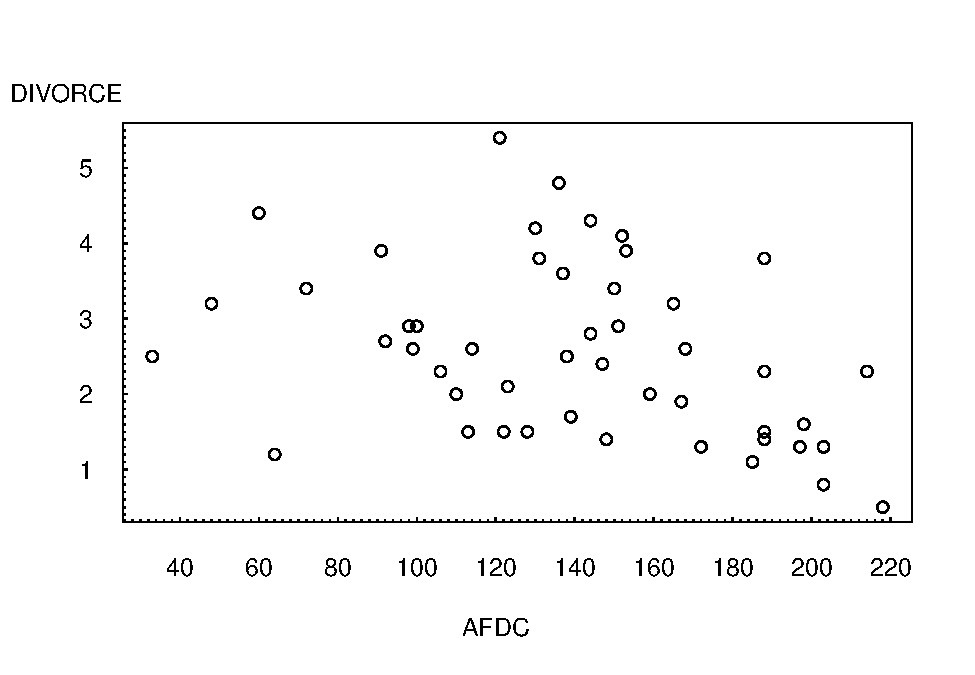
\includegraphics{LongPanelDataScripts_files/figure-latex/unnamed-chunk-6-1.pdf}

We can also plot 1975 data following the same method.

\begin{Shaded}
\begin{Highlighting}[]
\CommentTok{#  PLOT 1975 DATA ;}
\KeywordTok{plot}\NormalTok{(DIVORCE }\OperatorTok{~}\StringTok{ }\NormalTok{AFDC, }\DataTypeTok{subset=}\NormalTok{TIME }\OperatorTok\StringTok{ }\KeywordTok{c}\NormalTok{(}\DecValTok{2}\NormalTok{),}\DataTypeTok{data =}\NormalTok{ divorce,}\DataTypeTok{xaxt=}\StringTok{"n"}\NormalTok{, }\DataTypeTok{yaxt=}\StringTok{"n"}\NormalTok{,}\DataTypeTok{ylab=}\StringTok{""}\NormalTok{,}\DataTypeTok{xlab=}\StringTok{""}\NormalTok{)}
\KeywordTok{axis}\NormalTok{(}\DecValTok{2}\NormalTok{, }\DataTypeTok{at=}\KeywordTok{seq}\NormalTok{(}\DecValTok{2}\NormalTok{, }\DecValTok{9}\NormalTok{, }\DataTypeTok{by=}\DecValTok{1}\NormalTok{), }\DataTypeTok{las=}\DecValTok{1}\NormalTok{, }\DataTypeTok{font=}\DecValTok{10}\NormalTok{, }\DataTypeTok{cex=}\FloatTok{0.005}\NormalTok{, }\DataTypeTok{tck=}\FloatTok{0.01}\NormalTok{)}
\KeywordTok{axis}\NormalTok{(}\DecValTok{2}\NormalTok{, }\DataTypeTok{at=}\KeywordTok{seq}\NormalTok{(}\DecValTok{2}\NormalTok{, }\DecValTok{9}\NormalTok{, }\DataTypeTok{by=}\FloatTok{0.1}\NormalTok{), }\DataTypeTok{lab=}\NormalTok{F, }\DataTypeTok{tck=}\FloatTok{0.005}\NormalTok{)}
\KeywordTok{axis}\NormalTok{(}\DecValTok{1}\NormalTok{, }\DataTypeTok{at=}\KeywordTok{seq}\NormalTok{(}\DecValTok{0}\NormalTok{,}\DecValTok{400}\NormalTok{, }\DataTypeTok{by=}\DecValTok{100}\NormalTok{), }\DataTypeTok{font=}\DecValTok{10}\NormalTok{, }\DataTypeTok{cex=}\FloatTok{0.005}\NormalTok{, }\DataTypeTok{tck=}\FloatTok{0.01}\NormalTok{)}
\KeywordTok{axis}\NormalTok{(}\DecValTok{1}\NormalTok{, }\DataTypeTok{at=}\KeywordTok{seq}\NormalTok{(}\DecValTok{0}\NormalTok{,}\DecValTok{400}\NormalTok{, }\DataTypeTok{by=}\DecValTok{10}\NormalTok{), }\DataTypeTok{lab=}\NormalTok{F, }\DataTypeTok{tck=}\FloatTok{0.005}\NormalTok{)}
\KeywordTok{mtext}\NormalTok{(}\StringTok{"DIVORCE"}\NormalTok{, }\DataTypeTok{side=}\DecValTok{2}\NormalTok{, }\DataTypeTok{line=}\DecValTok{0}\NormalTok{, }\DataTypeTok{at=}\FloatTok{8.5}\NormalTok{, }\DataTypeTok{font=}\DecValTok{12}\NormalTok{, }\DataTypeTok{cex=}\DecValTok{1}\NormalTok{, }\DataTypeTok{las=}\DecValTok{1}\NormalTok{)}
\KeywordTok{mtext}\NormalTok{(}\StringTok{"AFDC"}\NormalTok{, }\DataTypeTok{side=}\DecValTok{1}\NormalTok{, }\DataTypeTok{line=}\DecValTok{3}\NormalTok{, }\DataTypeTok{at=}\DecValTok{200}\NormalTok{, }\DataTypeTok{font=}\DecValTok{12}\NormalTok{, }\DataTypeTok{cex=}\DecValTok{1}\NormalTok{)}
\end{Highlighting}
\end{Shaded}

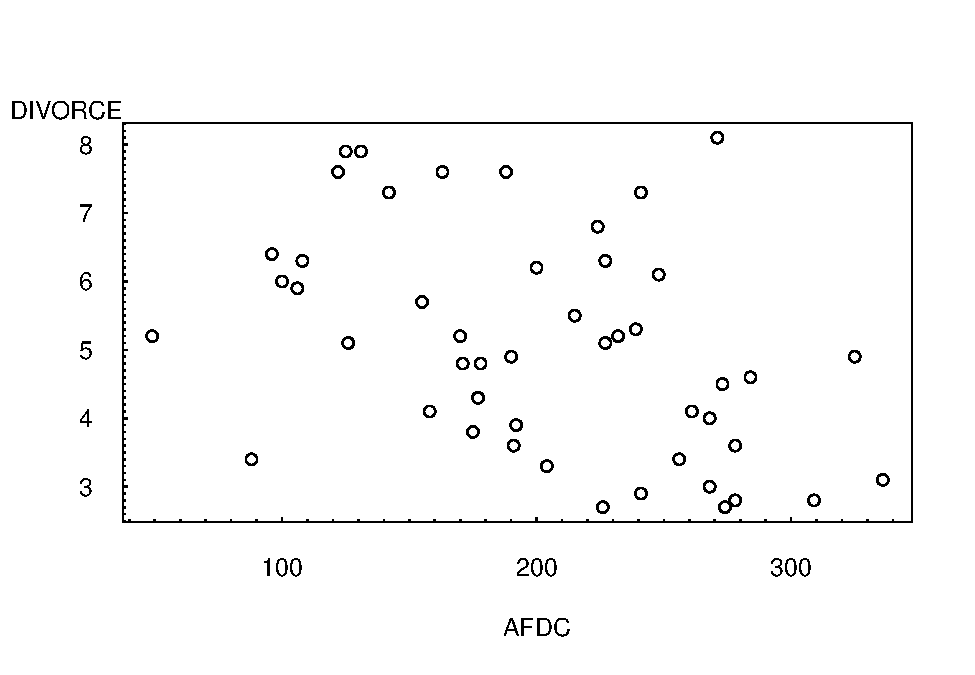
\includegraphics{LongPanelDataScripts_files/figure-latex/unnamed-chunk-7-1.pdf}

\hypertarget{figure-1.2-plot-of-divorce-rate-versus-afdc-payments-from-1965-and-1975.}{%
\subsection{Figure 1.2: Plot of divorce rate versus AFDC payments from 1965 and 1975.}\label{figure-1.2-plot-of-divorce-rate-versus-afdc-payments-from-1965-and-1975.}}

Figure 1.2 shows both the 1965 and 1975 data; a line connects the two observations within each state. These lines represent a change over time (dynamic), not a cross-sectional relationship.

\begin{Shaded}
\begin{Highlighting}[]
\KeywordTok{plot}\NormalTok{(DIVORCE }\OperatorTok{~}\StringTok{ }\NormalTok{AFDC, }\DataTypeTok{data =} \KeywordTok{subset}\NormalTok{(divorce, TIME }\OperatorTok\StringTok{ }\KeywordTok{c}\NormalTok{(}\DecValTok{1}\NormalTok{, }\DecValTok{2}\NormalTok{)), }\DataTypeTok{xaxt=}\StringTok{"n"}\NormalTok{, }\DataTypeTok{yaxt=}\StringTok{"n"}\NormalTok{,}\DataTypeTok{ylab=}\StringTok{""}\NormalTok{,}\DataTypeTok{xlab=}\StringTok{""}\NormalTok{)}
   \ControlFlowTok{for}\NormalTok{ (i }\ControlFlowTok{in}\NormalTok{ divorce}\OperatorTok{$}\NormalTok{STATE) \{}
    \KeywordTok{lines}\NormalTok{(DIVORCE }\OperatorTok{~}\StringTok{ }\NormalTok{AFDC, }\DataTypeTok{data =} \KeywordTok{subset}\NormalTok{(divorce, TIME }\OperatorTok\StringTok{ }\KeywordTok{c}\NormalTok{(}\DecValTok{1}\NormalTok{, }\DecValTok{2}\NormalTok{) }\OperatorTok{&}\StringTok{ }\NormalTok{STATE }\OperatorTok{==}\StringTok{ }\NormalTok{i)) \}}
\KeywordTok{axis}\NormalTok{(}\DecValTok{2}\NormalTok{, }\DataTypeTok{at=}\KeywordTok{seq}\NormalTok{(}\DecValTok{0}\NormalTok{, }\DecValTok{10}\NormalTok{, }\DataTypeTok{by=}\DecValTok{1}\NormalTok{), }\DataTypeTok{las=}\DecValTok{1}\NormalTok{, }\DataTypeTok{font=}\DecValTok{10}\NormalTok{, }\DataTypeTok{cex=}\FloatTok{0.005}\NormalTok{, }\DataTypeTok{tck=}\FloatTok{0.01}\NormalTok{)}
\KeywordTok{axis}\NormalTok{(}\DecValTok{2}\NormalTok{, }\DataTypeTok{at=}\KeywordTok{seq}\NormalTok{(}\DecValTok{0}\NormalTok{, }\DecValTok{10}\NormalTok{, }\DataTypeTok{by=}\FloatTok{0.1}\NormalTok{), }\DataTypeTok{lab=}\NormalTok{F, }\DataTypeTok{tck=}\FloatTok{0.005}\NormalTok{)}
\KeywordTok{axis}\NormalTok{(}\DecValTok{1}\NormalTok{, }\DataTypeTok{at=}\KeywordTok{seq}\NormalTok{(}\DecValTok{0}\NormalTok{,}\DecValTok{400}\NormalTok{, }\DataTypeTok{by=}\DecValTok{100}\NormalTok{), }\DataTypeTok{font=}\DecValTok{10}\NormalTok{, }\DataTypeTok{cex=}\FloatTok{0.005}\NormalTok{, }\DataTypeTok{tck=}\FloatTok{0.01}\NormalTok{)}
\KeywordTok{axis}\NormalTok{(}\DecValTok{1}\NormalTok{, }\DataTypeTok{at=}\KeywordTok{seq}\NormalTok{(}\DecValTok{0}\NormalTok{,}\DecValTok{400}\NormalTok{, }\DataTypeTok{by=}\DecValTok{10}\NormalTok{), }\DataTypeTok{lab=}\NormalTok{F, }\DataTypeTok{tck=}\FloatTok{0.005}\NormalTok{)}
\KeywordTok{mtext}\NormalTok{(}\StringTok{"DIVORCE"}\NormalTok{, }\DataTypeTok{side=}\DecValTok{2}\NormalTok{, }\DataTypeTok{line=}\DecValTok{0}\NormalTok{, }\DataTypeTok{at=}\FloatTok{8.5}\NormalTok{, }\DataTypeTok{font=}\DecValTok{12}\NormalTok{, }\DataTypeTok{cex=}\DecValTok{1}\NormalTok{, }\DataTypeTok{las=}\DecValTok{1}\NormalTok{)}
\KeywordTok{mtext}\NormalTok{(}\StringTok{"AFDC"}\NormalTok{, }\DataTypeTok{side=}\DecValTok{1}\NormalTok{, }\DataTypeTok{line=}\DecValTok{3}\NormalTok{, }\DataTypeTok{at=}\DecValTok{200}\NormalTok{, }\DataTypeTok{font=}\DecValTok{12}\NormalTok{, }\DataTypeTok{cex=}\DecValTok{1}\NormalTok{)}
\end{Highlighting}
\end{Shaded}

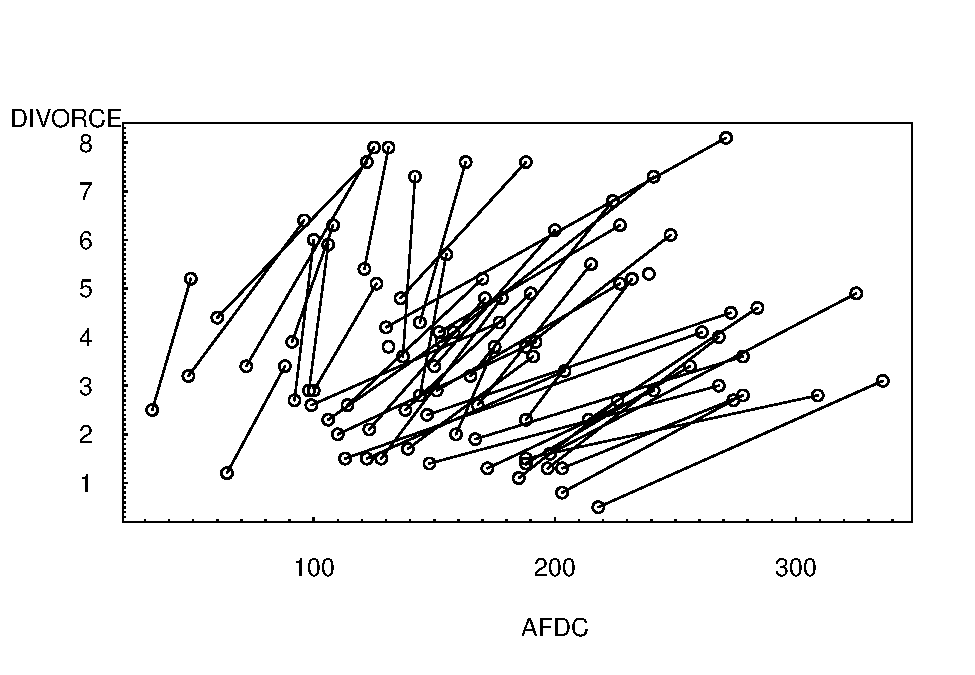
\includegraphics{LongPanelDataScripts_files/figure-latex/unnamed-chunk-8-1.pdf}

We can plot data for all years and connect the years.

\begin{Shaded}
\begin{Highlighting}[]
\CommentTok{#  PLOT ALL DATA, CONNECTING THE YEARS ;}
\KeywordTok{plot}\NormalTok{(DIVORCE }\OperatorTok{~}\StringTok{ }\NormalTok{AFDC, }\DataTypeTok{data =}\NormalTok{ divorce, }\DataTypeTok{xaxt=}\StringTok{"n"}\NormalTok{, }\DataTypeTok{yaxt=}\StringTok{"n"}\NormalTok{,}\DataTypeTok{ylab=}\StringTok{""}\NormalTok{,}\DataTypeTok{xlab=}\StringTok{""}\NormalTok{)}
  \ControlFlowTok{for}\NormalTok{ (i }\ControlFlowTok{in}\NormalTok{ divorce}\OperatorTok{$}\NormalTok{STATE) \{}
  \KeywordTok{lines}\NormalTok{(DIVORCE }\OperatorTok{~}\StringTok{ }\NormalTok{AFDC, }\DataTypeTok{data =} \KeywordTok{subset}\NormalTok{(divorce, STATE }\OperatorTok{==}\StringTok{ }\NormalTok{i)) \}}
\KeywordTok{axis}\NormalTok{(}\DecValTok{2}\NormalTok{, }\DataTypeTok{at=}\KeywordTok{seq}\NormalTok{(}\DecValTok{0}\NormalTok{, }\DecValTok{10}\NormalTok{, }\DataTypeTok{by=}\DecValTok{1}\NormalTok{), }\DataTypeTok{las=}\DecValTok{1}\NormalTok{, }\DataTypeTok{font=}\DecValTok{10}\NormalTok{, }\DataTypeTok{cex=}\FloatTok{0.005}\NormalTok{, }\DataTypeTok{tck=}\FloatTok{0.01}\NormalTok{)}
\KeywordTok{axis}\NormalTok{(}\DecValTok{2}\NormalTok{, }\DataTypeTok{at=}\KeywordTok{seq}\NormalTok{(}\DecValTok{0}\NormalTok{, }\DecValTok{10}\NormalTok{, }\DataTypeTok{by=}\FloatTok{0.1}\NormalTok{), }\DataTypeTok{lab=}\NormalTok{F, }\DataTypeTok{tck=}\FloatTok{0.005}\NormalTok{)}
\KeywordTok{axis}\NormalTok{(}\DecValTok{1}\NormalTok{, }\DataTypeTok{at=}\KeywordTok{seq}\NormalTok{(}\DecValTok{0}\NormalTok{,}\DecValTok{800}\NormalTok{, }\DataTypeTok{by=}\DecValTok{100}\NormalTok{), }\DataTypeTok{font=}\DecValTok{10}\NormalTok{, }\DataTypeTok{cex=}\FloatTok{0.005}\NormalTok{, }\DataTypeTok{tck=}\FloatTok{0.01}\NormalTok{)}
\KeywordTok{axis}\NormalTok{(}\DecValTok{1}\NormalTok{, }\DataTypeTok{at=}\KeywordTok{seq}\NormalTok{(}\DecValTok{0}\NormalTok{,}\DecValTok{800}\NormalTok{, }\DataTypeTok{by=}\DecValTok{10}\NormalTok{), }\DataTypeTok{lab=}\NormalTok{F, }\DataTypeTok{tck=}\FloatTok{0.005}\NormalTok{)}
\KeywordTok{mtext}\NormalTok{(}\StringTok{"DIVORCE"}\NormalTok{, }\DataTypeTok{side=}\DecValTok{2}\NormalTok{, }\DataTypeTok{line=}\DecValTok{0}\NormalTok{, }\DataTypeTok{at=}\DecValTok{10}\NormalTok{, }\DataTypeTok{font=}\DecValTok{12}\NormalTok{, }\DataTypeTok{cex=}\DecValTok{1}\NormalTok{, }\DataTypeTok{las=}\DecValTok{1}\NormalTok{)}
\KeywordTok{mtext}\NormalTok{(}\StringTok{"AFDC"}\NormalTok{, }\DataTypeTok{side=}\DecValTok{1}\NormalTok{, }\DataTypeTok{line=}\DecValTok{3}\NormalTok{, }\DataTypeTok{at=}\DecValTok{400}\NormalTok{, }\DataTypeTok{font=}\DecValTok{12}\NormalTok{, }\DataTypeTok{cex=}\DecValTok{1}\NormalTok{)}
\end{Highlighting}
\end{Shaded}

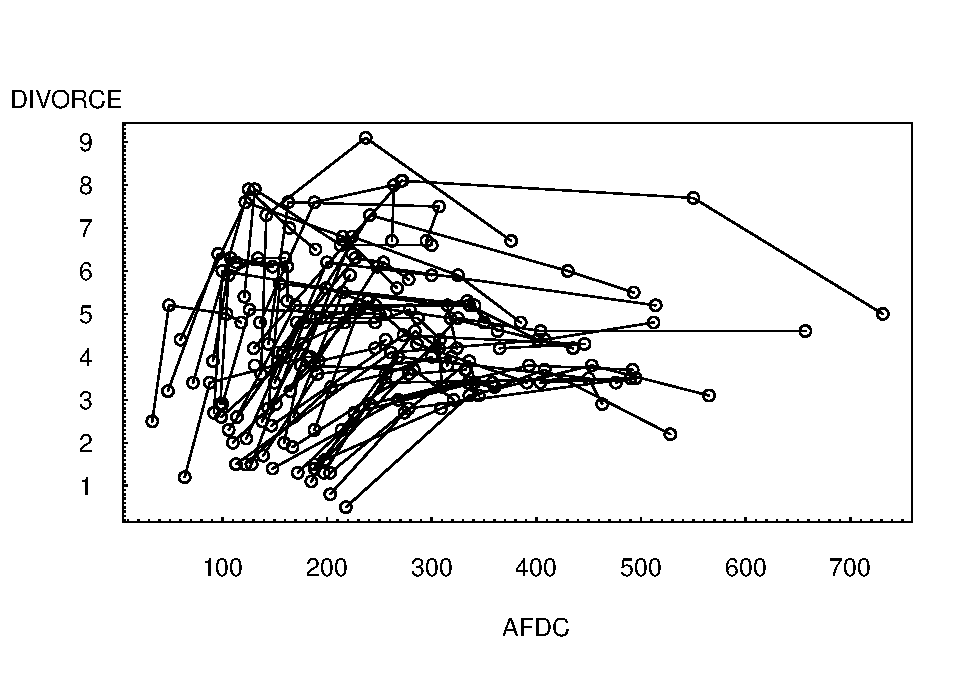
\includegraphics{LongPanelDataScripts_files/figure-latex/unnamed-chunk-9-1.pdf}

We can also look at the multiple time series plot by the \texttt{STATE}.

\begin{Shaded}
\begin{Highlighting}[]
\CommentTok{#  MULTIPLE TIME SERIES PLOT  ;}
\NormalTok{divorce}\OperatorTok{$}\NormalTok{YEAR=divorce}\OperatorTok{$}\NormalTok{TIME}\OperatorTok{*}\DecValTok{10}\OperatorTok{+}\DecValTok{1955}
\KeywordTok{plot}\NormalTok{(DIVORCE }\OperatorTok{~}\StringTok{ }\NormalTok{YEAR, }\DataTypeTok{data =}\NormalTok{ divorce, }\DataTypeTok{xaxt=}\StringTok{"n"}\NormalTok{, }\DataTypeTok{yaxt=}\StringTok{"n"}\NormalTok{,}\DataTypeTok{ylab=}\StringTok{""}\NormalTok{,}\DataTypeTok{xlab=}\StringTok{""}\NormalTok{)}
   \ControlFlowTok{for}\NormalTok{ (i }\ControlFlowTok{in}\NormalTok{ divorce}\OperatorTok{$}\NormalTok{STATE) \{}
   \KeywordTok{lines}\NormalTok{(DIVORCE }\OperatorTok{~}\StringTok{ }\NormalTok{YEAR, }\DataTypeTok{data =} \KeywordTok{subset}\NormalTok{(divorce, STATE }\OperatorTok{==}\StringTok{ }\NormalTok{i)) \}}
\KeywordTok{axis}\NormalTok{(}\DecValTok{2}\NormalTok{, }\DataTypeTok{at=}\KeywordTok{seq}\NormalTok{(}\DecValTok{0}\NormalTok{, }\DecValTok{10}\NormalTok{, }\DataTypeTok{by=}\DecValTok{1}\NormalTok{), }\DataTypeTok{las=}\DecValTok{1}\NormalTok{, }\DataTypeTok{font=}\DecValTok{10}\NormalTok{, }\DataTypeTok{cex=}\FloatTok{0.005}\NormalTok{, }\DataTypeTok{tck=}\FloatTok{0.01}\NormalTok{)}
\KeywordTok{axis}\NormalTok{(}\DecValTok{2}\NormalTok{, }\DataTypeTok{at=}\KeywordTok{seq}\NormalTok{(}\DecValTok{0}\NormalTok{, }\DecValTok{10}\NormalTok{, }\DataTypeTok{by=}\FloatTok{0.1}\NormalTok{), }\DataTypeTok{lab=}\NormalTok{F, }\DataTypeTok{tck=}\FloatTok{0.005}\NormalTok{)}
\KeywordTok{axis}\NormalTok{(}\DecValTok{1}\NormalTok{, }\DataTypeTok{at=}\KeywordTok{seq}\NormalTok{(}\DecValTok{1965}\NormalTok{,}\DecValTok{1995}\NormalTok{, }\DataTypeTok{by=}\DecValTok{10}\NormalTok{), }\DataTypeTok{font=}\DecValTok{10}\NormalTok{, }\DataTypeTok{cex=}\FloatTok{0.005}\NormalTok{, }\DataTypeTok{tck=}\FloatTok{0.01}\NormalTok{)}
\KeywordTok{axis}\NormalTok{(}\DecValTok{1}\NormalTok{, }\DataTypeTok{at=}\KeywordTok{seq}\NormalTok{(}\DecValTok{1964}\NormalTok{,}\DecValTok{2000}\NormalTok{, }\DataTypeTok{by=}\DecValTok{1}\NormalTok{), }\DataTypeTok{lab=}\NormalTok{F, }\DataTypeTok{tck=}\FloatTok{0.005}\NormalTok{)}
\KeywordTok{mtext}\NormalTok{(}\StringTok{"DIVORCE"}\NormalTok{, }\DataTypeTok{side=}\DecValTok{2}\NormalTok{, }\DataTypeTok{line=}\DecValTok{0}\NormalTok{, }\DataTypeTok{at=}\DecValTok{10}\NormalTok{, }\DataTypeTok{font=}\DecValTok{12}\NormalTok{, }\DataTypeTok{cex=}\DecValTok{1}\NormalTok{, }\DataTypeTok{las=}\DecValTok{1}\NormalTok{)}
\KeywordTok{mtext}\NormalTok{(}\StringTok{"YEAR"}\NormalTok{, }\DataTypeTok{side=}\DecValTok{1}\NormalTok{, }\DataTypeTok{line=}\DecValTok{3}\NormalTok{, }\DataTypeTok{at=}\DecValTok{1980}\NormalTok{, }\DataTypeTok{font=}\DecValTok{12}\NormalTok{, }\DataTypeTok{cex=}\DecValTok{1}\NormalTok{)}
\end{Highlighting}
\end{Shaded}

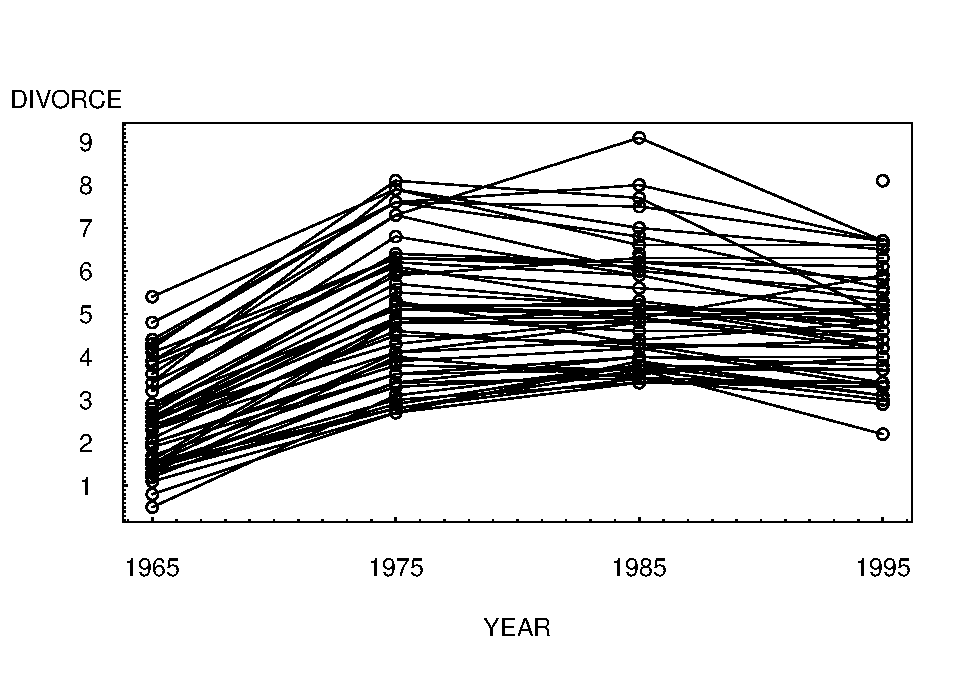
\includegraphics{LongPanelDataScripts_files/figure-latex/unnamed-chunk-10-1.pdf}

\hypertarget{fixed-effects-models}{%
\chapter{Fixed-Effects Models}\label{fixed-effects-models}}

\hypertarget{import-data-1}{%
\section{Import Data}\label{import-data-1}}

We consider T=6 years, 1990-1995, of data for inpatient hospital charges that are covered by the Medicare program. The data were obtained from the Health Care Financing Administration, Bureau of Data Management and Strategy. To illustrate, in 1995 the total covered charges were \$157.8 billions for twelve million discharges. For this analysis, we use state as the subject, or risk class. Thus, we consider n=54 states that include the 50 states in the Union, the District of Columbia, Virgin Islands, Puerto Rico and an unspecified ``other'' category.

\begin{longtable}[]{@{}ll@{}}
\toprule
\begin{minipage}[b]{0.09\columnwidth}\raggedright
Variable\strut
\end{minipage} & \begin{minipage}[b]{0.85\columnwidth}\raggedright
Description\strut
\end{minipage}\tabularnewline
\midrule
\endhead
\begin{minipage}[t]{0.09\columnwidth}\raggedright
STATE\strut
\end{minipage} & \begin{minipage}[t]{0.85\columnwidth}\raggedright
State identifier, 1-54\strut
\end{minipage}\tabularnewline
\begin{minipage}[t]{0.09\columnwidth}\raggedright
YEAR\strut
\end{minipage} & \begin{minipage}[t]{0.85\columnwidth}\raggedright
Year identifier, 1-6\strut
\end{minipage}\tabularnewline
\begin{minipage}[t]{0.09\columnwidth}\raggedright
TOT\_CHG\strut
\end{minipage} & \begin{minipage}[t]{0.85\columnwidth}\raggedright
Total hospital charges, in millions of dollars.\strut
\end{minipage}\tabularnewline
\begin{minipage}[t]{0.09\columnwidth}\raggedright
COV\_CHG\strut
\end{minipage} & \begin{minipage}[t]{0.85\columnwidth}\raggedright
Total hospital charges covered by Medicare, in millions of dollars.\strut
\end{minipage}\tabularnewline
\begin{minipage}[t]{0.09\columnwidth}\raggedright
MED\_REIM\strut
\end{minipage} & \begin{minipage}[t]{0.85\columnwidth}\raggedright
Total hospital charges reimbursed by the Medicare program, in millions of dollars.\strut
\end{minipage}\tabularnewline
\begin{minipage}[t]{0.09\columnwidth}\raggedright
TOT\_D\strut
\end{minipage} & \begin{minipage}[t]{0.85\columnwidth}\raggedright
Total number of hospitals stays, in days.\strut
\end{minipage}\tabularnewline
\begin{minipage}[t]{0.09\columnwidth}\raggedright
NUM\_DSHG\strut
\end{minipage} & \begin{minipage}[t]{0.85\columnwidth}\raggedright
Number discharged, in thousands.\strut
\end{minipage}\tabularnewline
\begin{minipage}[t]{0.09\columnwidth}\raggedright
AVE\_T\_D\strut
\end{minipage} & \begin{minipage}[t]{0.85\columnwidth}\raggedright
Average hospital stay per discharge in days.\strut
\end{minipage}\tabularnewline
\bottomrule
\end{longtable}

\begin{Shaded}
\begin{Highlighting}[]
\CommentTok{#  "\textbackslash{}t"  INDICATES SEPARATED BY TABLES  ;}
\NormalTok{Medicare  =}\StringTok{ }\KeywordTok{read.table}\NormalTok{(}\StringTok{"TXTData/Medicare.txt"}\NormalTok{, }\DataTypeTok{sep =}\StringTok{"}\CharTok{\textbackslash{}t}\StringTok{"}\NormalTok{, }\DataTypeTok{quote =} \StringTok{""}\NormalTok{,}\DataTypeTok{header=}\OtherTok{TRUE}\NormalTok{)}

\CommentTok{# Medicare = read.table(choose.files(), sep ="\textbackslash{}t", quote = "",header=TRUE)}
\end{Highlighting}
\end{Shaded}

Let's have a look at the dataset. The names of variables and the first 8 rows observations.

\begin{Shaded}
\begin{Highlighting}[]
\CommentTok{#  PROVIDES THE NAMES IN THE FILE AND LISTS THE FIRST 8 OBSERVATIONS  ;}
\KeywordTok{names}\NormalTok{ (Medicare)}
\end{Highlighting}
\end{Shaded}

\begin{verbatim}
[1] "STATE"    "YEAR"     "TOT_CHG"  "COV_CHG"  "MED_REIB" "TOT_D"   
[7] "NUM_DCHG" "AVE_T_D"  "NMSTATE" 
\end{verbatim}

\begin{Shaded}
\begin{Highlighting}[]
\NormalTok{Medicare [}\DecValTok{1}\OperatorTok{:}\DecValTok{8}\NormalTok{, ]}
\end{Highlighting}
\end{Shaded}

\begin{verbatim}
  STATE YEAR    TOT_CHG    COV_CHG   MED_REIB   TOT_D NUM_DCHG AVE_T_D
1     1    1 2211617271 2170240349  972752944 1932673   230015       8
2     1    2 2523987347 2468263759 1046016144 1936939   234739       8
3     1    3 2975969979 2922611694 1205791592 2016354   245027       8
4     1    4 3194595003 3149745611 1307982985 1948427   243947       8
5     1    5 3417704863 3384305357 1376211788 1926335   258384       7
6     1    6 3519375275 3492635576 1466220936 1847216   261738       7
7     2    1   64747759   62242279   42083051   51923     6636       8
8     2    2   70600503   67579913   46928596   53051     6940       8
  NMSTATE
1      AL
2      AL
3      AL
4      AL
5      AL
6      AL
7      AK
8      AK
\end{verbatim}

Then we need to create some other variables for later use.

\begin{Shaded}
\begin{Highlighting}[]
\CommentTok{#  CREATE OTHER VARIABLES;}
\CommentTok{# Firstly, we need change the names of existing variables.}
\KeywordTok{names}\NormalTok{(Medicare)[}\KeywordTok{names}\NormalTok{(Medicare)}\OperatorTok{==}\StringTok{"TOT_CHG"}\NormalTok{]=}\StringTok{"TOT.CHG"}\NormalTok{;}
\KeywordTok{names}\NormalTok{(Medicare)[}\KeywordTok{names}\NormalTok{(Medicare)}\OperatorTok{==}\StringTok{"COV_CHG"}\NormalTok{]=}\StringTok{"COV.CHG"}\NormalTok{;}
\KeywordTok{names}\NormalTok{(Medicare)[}\KeywordTok{names}\NormalTok{(Medicare)}\OperatorTok{==}\StringTok{"MED_REIB"}\NormalTok{]=}\StringTok{"MED.REIB"}\NormalTok{;}
\KeywordTok{names}\NormalTok{(Medicare)[}\KeywordTok{names}\NormalTok{(Medicare)}\OperatorTok{==}\StringTok{"TOT_D"}\NormalTok{]=}\StringTok{"TOT.D"}\NormalTok{;}
\KeywordTok{names}\NormalTok{(Medicare)[}\KeywordTok{names}\NormalTok{(Medicare)}\OperatorTok{==}\StringTok{"NUM_DCHG"}\NormalTok{]=}\StringTok{"NUM.DCHG"}\NormalTok{;}
\KeywordTok{names}\NormalTok{(Medicare)[}\KeywordTok{names}\NormalTok{(Medicare)}\OperatorTok{==}\StringTok{"AVE_T_D"}\NormalTok{]=}\StringTok{"AVE.T.D"}\NormalTok{;}

\NormalTok{Medicare}\OperatorTok{$}\NormalTok{AVE.DAYS=}\StringTok{ }\NormalTok{Medicare}\OperatorTok{$}\NormalTok{TOT.D}\OperatorTok{/}\NormalTok{Medicare}\OperatorTok{$}\NormalTok{NUM.DCHG}
\NormalTok{Medicare}\OperatorTok{$}\NormalTok{CCPD=Medicare}\OperatorTok{$}\NormalTok{COV.CHG}\OperatorTok{/}\NormalTok{Medicare}\OperatorTok{$}\NormalTok{NUM.DCHG}
\NormalTok{Medicare}\OperatorTok{$}\NormalTok{NUM.DCHG=Medicare}\OperatorTok{$}\NormalTok{NUM.DCHG}\OperatorTok{/}\DecValTok{1000}
\KeywordTok{str}\NormalTok{ (Medicare)}
\end{Highlighting}
\end{Shaded}

\begin{verbatim}
'data.frame':   324 obs. of  11 variables:
 $ STATE   : int  1 1 1 1 1 1 2 2 2 2 ...
 $ YEAR    : int  1 2 3 4 5 6 1 2 3 4 ...
 $ TOT.CHG : num  2.21e+09 2.52e+09 2.98e+09 3.19e+09 3.42e+09 ...
 $ COV.CHG : num  2.17e+09 2.47e+09 2.92e+09 3.15e+09 3.38e+09 ...
 $ MED.REIB: num  9.73e+08 1.05e+09 1.21e+09 1.31e+09 1.38e+09 ...
 $ TOT.D   : int  1932673 1936939 2016354 1948427 1926335 1847216 51923 53051 55191 53329 ...
 $ NUM.DCHG: num  230 235 245 244 258 ...
 $ AVE.T.D : int  8 8 8 8 7 7 8 8 7 7 ...
 $ NMSTATE : Factor w/ 54 levels "AK","AL","AR",..: 2 2 2 2 2 2 1 1 1 1 ...
 $ AVE.DAYS: num  8.4 8.25 8.23 7.99 7.46 ...
 $ CCPD    : num  9435 10515 11928 12912 13098 ...
\end{verbatim}

Some summary statistics of \texttt{CCPD}, \texttt{NUM.DCHG}, \texttt{AVE\textgreater{}DAYS}, \texttt{YEAR} in each year.

\begin{Shaded}
\begin{Highlighting}[]
\KeywordTok{library}\NormalTok{(nlme)}
\KeywordTok{attach}\NormalTok{(Medicare)}
\CommentTok{#  SUMMARY STATISTICS ;}
\KeywordTok{dim}\NormalTok{(Medicare)}
\end{Highlighting}
\end{Shaded}

\begin{verbatim}
[1] 324  11
\end{verbatim}

\begin{Shaded}
\begin{Highlighting}[]
\KeywordTok{summary}\NormalTok{(Medicare[, }\KeywordTok{c}\NormalTok{(}\StringTok{"CCPD"}\NormalTok{, }\StringTok{"NUM.DCHG"}\NormalTok{, }\StringTok{"AVE.DAYS"}\NormalTok{ )])}
\end{Highlighting}
\end{Shaded}

\begin{verbatim}
      CCPD          NUM.DCHG          AVE.DAYS     
 Min.   : 2966   Min.   :  0.515   Min.   : 5.119  
 1st Qu.: 8537   1st Qu.: 42.715   1st Qu.: 7.162  
 Median :10073   Median :144.282   Median : 8.067  
 Mean   :10483   Mean   :210.731   Mean   : 8.542  
 3rd Qu.:12059   3rd Qu.:282.884   3rd Qu.: 8.988  
 Max.   :21500   Max.   :908.593   Max.   :60.251  
\end{verbatim}

\begin{Shaded}
\begin{Highlighting}[]
\KeywordTok{gsummary}\NormalTok{(Medicare[, }\KeywordTok{c}\NormalTok{(}\StringTok{"CCPD"}\NormalTok{, }\StringTok{"NUM.DCHG"}\NormalTok{, }\StringTok{"AVE.DAYS"}\NormalTok{, }\StringTok{"YEAR"}\NormalTok{)], }\DataTypeTok{groups =}\NormalTok{ YEAR, }\DataTypeTok{FUN=}\NormalTok{sd)}
\end{Highlighting}
\end{Shaded}

\begin{verbatim}
      CCPD NUM.DCHG AVE.DAYS YEAR
1 2466.685 202.9918 2.077437    1
2 2711.568 210.3791 7.231312    2
3 3041.274 218.9225 1.858683    3
4 3259.846 219.8253 2.112467    4
5 3345.970 226.7783 1.728882    5
6 3277.985 229.4583 1.444423    6
\end{verbatim}

\begin{Shaded}
\begin{Highlighting}[]
\KeywordTok{gsummary}\NormalTok{(Medicare[, }\KeywordTok{c}\NormalTok{(}\StringTok{"CCPD"}\NormalTok{, }\StringTok{"NUM.DCHG"}\NormalTok{, }\StringTok{"AVE.DAYS"}\NormalTok{, }\StringTok{"YEAR"}\NormalTok{)], }\DataTypeTok{groups =}\NormalTok{ YEAR, }\DataTypeTok{FUN=}\NormalTok{mean)}
\end{Highlighting}
\end{Shaded}

\begin{verbatim}
       CCPD NUM.DCHG AVE.DAYS YEAR
1  8503.168 197.7274 9.048565    1
2  9472.746 203.1443 9.823055    2
3 10443.285 210.8941 8.619240    3
4 11159.680 211.2479 8.522619    4
5 11522.826 218.8690 7.898816    5
6 11796.768 222.5059 7.342360    6
\end{verbatim}

\begin{Shaded}
\begin{Highlighting}[]
\KeywordTok{gsummary}\NormalTok{(Medicare[, }\KeywordTok{c}\NormalTok{(}\StringTok{"CCPD"}\NormalTok{, }\StringTok{"NUM.DCHG"}\NormalTok{, }\StringTok{"AVE.DAYS"}\NormalTok{, }\StringTok{"YEAR"}\NormalTok{)], }\DataTypeTok{groups =}\NormalTok{ YEAR, }\DataTypeTok{FUN=}\NormalTok{median)}
\end{Highlighting}
\end{Shaded}

\begin{verbatim}
       CCPD NUM.DCHG AVE.DAYS YEAR
1  7991.927 142.5880 8.533565    1
2  9113.473 142.6935 8.570416    2
3 10055.416 143.2515 8.363435    3
4 10666.865 143.6720 8.112863    4
5 10955.142 150.0765 7.560945    5
6 11171.080 152.6960 7.143355    6
\end{verbatim}

\begin{Shaded}
\begin{Highlighting}[]
\KeywordTok{gsummary}\NormalTok{(Medicare[, }\KeywordTok{c}\NormalTok{(}\StringTok{"CCPD"}\NormalTok{, }\StringTok{"NUM.DCHG"}\NormalTok{, }\StringTok{"AVE.DAYS"}\NormalTok{, }\StringTok{"YEAR"}\NormalTok{)], }\DataTypeTok{groups =}\NormalTok{ YEAR, }\DataTypeTok{FUN=}\NormalTok{min)}
\end{Highlighting}
\end{Shaded}

\begin{verbatim}
      CCPD NUM.DCHG AVE.DAYS YEAR
1 3228.989    0.528 6.326762    1
2 2966.117    0.515 6.143628    2
3 3324.113    0.653 5.830248    3
4 4137.776    0.969 5.830995    4
5 4354.526    1.156 5.378061    5
6 5058.371    1.059 5.118937    6
\end{verbatim}

\begin{Shaded}
\begin{Highlighting}[]
\KeywordTok{gsummary}\NormalTok{(Medicare[, }\KeywordTok{c}\NormalTok{(}\StringTok{"CCPD"}\NormalTok{, }\StringTok{"NUM.DCHG"}\NormalTok{, }\StringTok{"AVE.DAYS"}\NormalTok{, }\StringTok{"YEAR"}\NormalTok{)], }\DataTypeTok{groups =}\NormalTok{ YEAR, }\DataTypeTok{FUN=}\NormalTok{max)}
\end{Highlighting}
\end{Shaded}

\begin{verbatim}
      CCPD NUM.DCHG AVE.DAYS YEAR
1 16484.77  849.372 17.47888    1
2 17636.51  885.919 60.25108    2
3 19814.09  908.593 16.35045    3
4 21121.55  894.216 17.13484    4
5 21500.29  905.615 14.38731    5
6 21031.58  902.479 12.79622    6
\end{verbatim}

See the box plots of different variables in each year.

\begin{Shaded}
\begin{Highlighting}[]
\CommentTok{#  ATTACH THE DATA SET FOR SOME PRELIMINARLY LOOKS;}
\KeywordTok{attach}\NormalTok{ (Medicare)}
\end{Highlighting}
\end{Shaded}

\begin{verbatim}
The following objects are masked from Medicare (pos = 3):

    AVE.DAYS, AVE.T.D, CCPD, COV.CHG, MED.REIB, NMSTATE, NUM.DCHG,
    STATE, TOT.CHG, TOT.D, YEAR
\end{verbatim}

\begin{Shaded}
\begin{Highlighting}[]
\NormalTok{Medicare}\OperatorTok{$}\NormalTok{YEAR=Medicare}\OperatorTok{$}\NormalTok{YEAR}\OperatorTok{+}\DecValTok{1989}
\KeywordTok{boxplot}\NormalTok{ (CCPD }\OperatorTok{~}\StringTok{ }\NormalTok{YEAR)}
\end{Highlighting}
\end{Shaded}

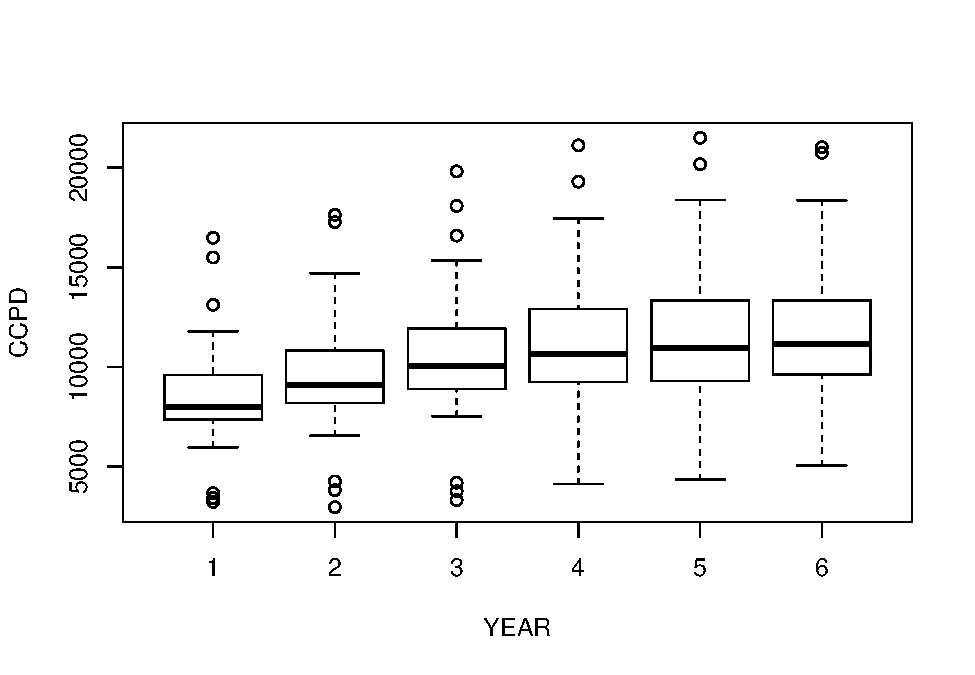
\includegraphics{LongPanelDataScripts_files/figure-latex/unnamed-chunk-15-1.pdf}

\begin{Shaded}
\begin{Highlighting}[]
\KeywordTok{boxplot}\NormalTok{ (NUM.DCHG }\OperatorTok{~}\StringTok{ }\NormalTok{YEAR)}
\end{Highlighting}
\end{Shaded}

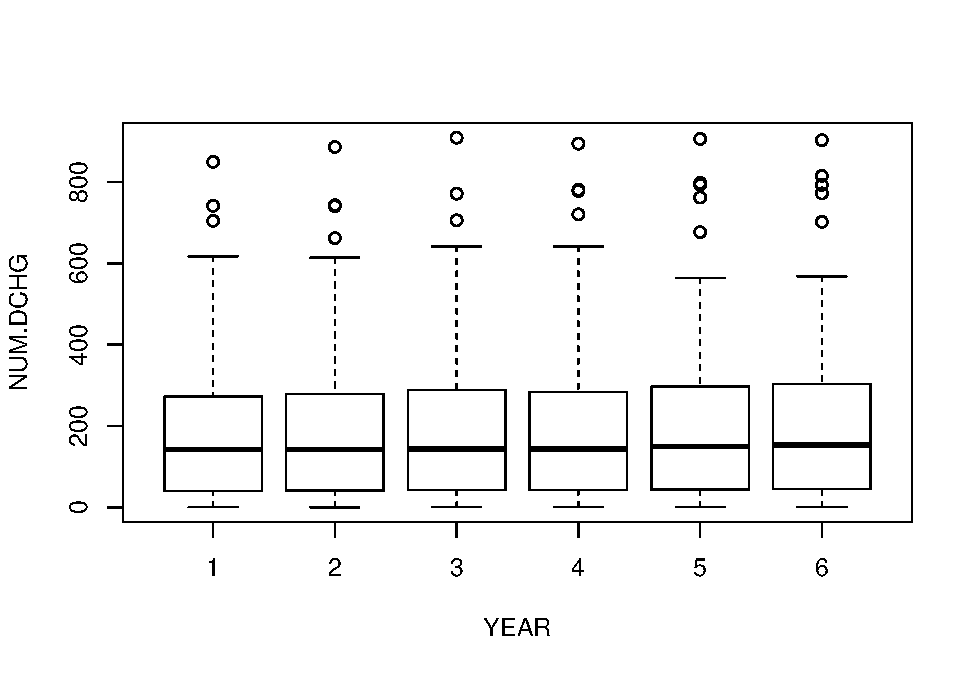
\includegraphics{LongPanelDataScripts_files/figure-latex/unnamed-chunk-15-2.pdf}

\begin{Shaded}
\begin{Highlighting}[]
\KeywordTok{boxplot}\NormalTok{ (AVE.DAYS }\OperatorTok{~}\StringTok{ }\NormalTok{YEAR)}
\end{Highlighting}
\end{Shaded}

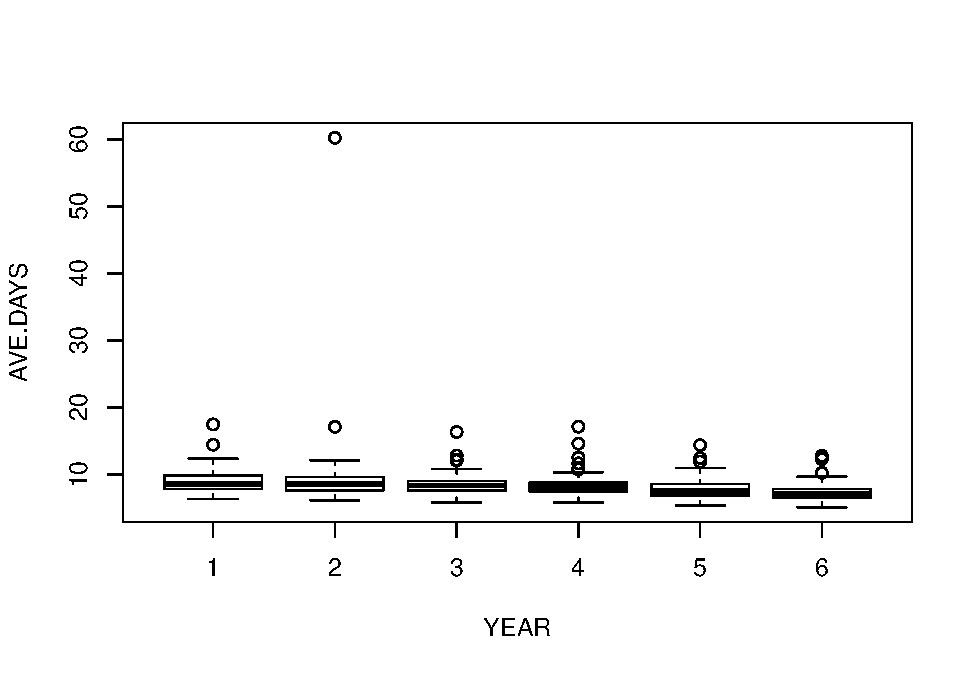
\includegraphics{LongPanelDataScripts_files/figure-latex/unnamed-chunk-15-3.pdf}

\hypertarget{example-2.2-medicare-hospital-costs-page-26}{%
\section{Example 2.2: Medicare Hospital Costs (Page 26)}\label{example-2.2-medicare-hospital-costs-page-26}}

\hypertarget{figure-2.1-ccpd-vs-year-multiple-time-series-plot}{%
\subsection{FIGURE 2.1: CCPD vs YEAR; multiple time series plot}\label{figure-2.1-ccpd-vs-year-multiple-time-series-plot}}

Figure 2.1 illustrates the multiple time-series plot. Here, we see that not only are overall claims increasing but also that claims increase for each state.

\begin{Shaded}
\begin{Highlighting}[]
\KeywordTok{plot}\NormalTok{(CCPD }\OperatorTok{~}\StringTok{ }\NormalTok{YEAR, }\DataTypeTok{data =}\NormalTok{ Medicare, }\DataTypeTok{xaxt=}\StringTok{"n"}\NormalTok{, }\DataTypeTok{yaxt=}\StringTok{"n"}\NormalTok{, }\DataTypeTok{ylab=}\StringTok{""}\NormalTok{, }\DataTypeTok{xlab=}\StringTok{""}\NormalTok{)}
 \ControlFlowTok{for}\NormalTok{ (i }\ControlFlowTok{in}\NormalTok{ Medicare}\OperatorTok{$}\NormalTok{STATE) \{}
 \KeywordTok{lines}\NormalTok{(CCPD }\OperatorTok{~}\StringTok{ }\NormalTok{YEAR, }\DataTypeTok{data =} \KeywordTok{subset}\NormalTok{(Medicare, STATE }\OperatorTok{==}\StringTok{ }\NormalTok{i)) \}}
\KeywordTok{axis}\NormalTok{(}\DecValTok{2}\NormalTok{, }\DataTypeTok{at=}\KeywordTok{seq}\NormalTok{(}\DecValTok{0}\NormalTok{, }\DecValTok{22000}\NormalTok{, }\DataTypeTok{by=}\DecValTok{2000}\NormalTok{), }\DataTypeTok{las=}\DecValTok{1}\NormalTok{, }\DataTypeTok{font=}\DecValTok{10}\NormalTok{, }\DataTypeTok{cex=}\FloatTok{0.005}\NormalTok{, }\DataTypeTok{tck=}\FloatTok{0.01}\NormalTok{)}
\KeywordTok{axis}\NormalTok{(}\DecValTok{1}\NormalTok{, }\DataTypeTok{at=}\KeywordTok{seq}\NormalTok{(}\DecValTok{1990}\NormalTok{,}\DecValTok{1995}\NormalTok{, }\DataTypeTok{by=}\DecValTok{1}\NormalTok{), }\DataTypeTok{font=}\DecValTok{10}\NormalTok{, }\DataTypeTok{cex=}\FloatTok{0.005}\NormalTok{, }\DataTypeTok{tck=}\FloatTok{0.01}\NormalTok{)}
\KeywordTok{mtext}\NormalTok{(}\StringTok{"CCPD"}\NormalTok{, }\DataTypeTok{side=}\DecValTok{2}\NormalTok{, }\DataTypeTok{line=}\DecValTok{0}\NormalTok{, }\DataTypeTok{at=}\DecValTok{23000}\NormalTok{, }\DataTypeTok{font=}\DecValTok{12}\NormalTok{, }\DataTypeTok{cex=}\DecValTok{1}\NormalTok{, }\DataTypeTok{las=}\DecValTok{1}\NormalTok{)}
\KeywordTok{mtext}\NormalTok{(}\StringTok{"YEAR"}\NormalTok{, }\DataTypeTok{side=}\DecValTok{1}\NormalTok{, }\DataTypeTok{line=}\DecValTok{3}\NormalTok{, }\DataTypeTok{at=}\FloatTok{1992.5}\NormalTok{, }\DataTypeTok{font=}\DecValTok{12}\NormalTok{, }\DataTypeTok{cex=}\DecValTok{1}\NormalTok{)}
\end{Highlighting}
\end{Shaded}

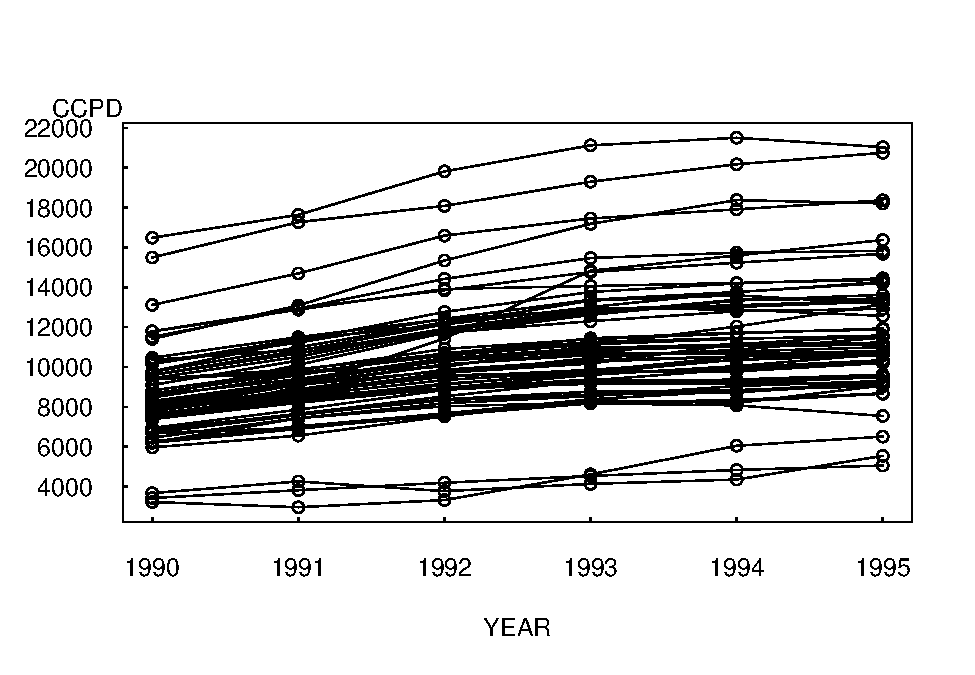
\includegraphics{LongPanelDataScripts_files/figure-latex/unnamed-chunk-16-1.pdf}

\hypertarget{figure-2.2-ccpd-vs-num.dchg}{%
\subsection{FIGURE 2.2: CCPD vs NUM.DCHG}\label{figure-2.2-ccpd-vs-num.dchg}}

Figure 2.2 illustrates the scatter plot with symbols. This plot ofCCPD versus number ofdischarges, connecting observations over time, shows a positive overall relationship between CCPD and the number of discharges.

\begin{Shaded}
\begin{Highlighting}[]
\KeywordTok{plot}\NormalTok{(CCPD }\OperatorTok{~}\StringTok{ }\NormalTok{NUM.DCHG, }\DataTypeTok{data =}\NormalTok{ Medicare, }\DataTypeTok{xaxt=}\StringTok{"n"}\NormalTok{, }\DataTypeTok{yaxt=}\StringTok{"n"}\NormalTok{, }\DataTypeTok{ylab=}\StringTok{""}\NormalTok{, }\DataTypeTok{xlab=}\StringTok{""}\NormalTok{)}
\ControlFlowTok{for}\NormalTok{ (i }\ControlFlowTok{in}\NormalTok{ Medicare}\OperatorTok{$}\NormalTok{STATE) \{}
 \KeywordTok{lines}\NormalTok{(CCPD }\OperatorTok{~}\StringTok{ }\NormalTok{NUM.DCHG, }\DataTypeTok{data =} \KeywordTok{subset}\NormalTok{(Medicare, STATE }\OperatorTok{==}\StringTok{ }\NormalTok{i)) \}}
\KeywordTok{axis}\NormalTok{(}\DecValTok{2}\NormalTok{, }\DataTypeTok{at=}\KeywordTok{seq}\NormalTok{(}\DecValTok{0}\NormalTok{, }\DecValTok{22000}\NormalTok{, }\DataTypeTok{by=}\DecValTok{2000}\NormalTok{), }\DataTypeTok{las=}\DecValTok{1}\NormalTok{, }\DataTypeTok{font=}\DecValTok{10}\NormalTok{, }\DataTypeTok{cex=}\FloatTok{0.005}\NormalTok{, }\DataTypeTok{tck=}\FloatTok{0.01}\NormalTok{)}
\KeywordTok{axis}\NormalTok{(}\DecValTok{2}\NormalTok{, }\DataTypeTok{at=}\KeywordTok{seq}\NormalTok{(}\DecValTok{0}\NormalTok{, }\DecValTok{22000}\NormalTok{, }\DataTypeTok{by=}\DecValTok{200}\NormalTok{), }\DataTypeTok{lab=}\NormalTok{F, }\DataTypeTok{tck=}\FloatTok{0.005}\NormalTok{)}
\KeywordTok{axis}\NormalTok{(}\DecValTok{1}\NormalTok{, }\DataTypeTok{at=}\KeywordTok{seq}\NormalTok{(}\DecValTok{0}\NormalTok{,}\DecValTok{1200}\NormalTok{, }\DataTypeTok{by=}\DecValTok{200}\NormalTok{), }\DataTypeTok{font=}\DecValTok{10}\NormalTok{, }\DataTypeTok{cex=}\FloatTok{0.005}\NormalTok{, }\DataTypeTok{tck=}\FloatTok{0.01}\NormalTok{)}
\KeywordTok{axis}\NormalTok{(}\DecValTok{1}\NormalTok{, }\DataTypeTok{at=}\KeywordTok{seq}\NormalTok{(}\DecValTok{0}\NormalTok{,}\DecValTok{1200}\NormalTok{, }\DataTypeTok{by=}\DecValTok{20}\NormalTok{), }\DataTypeTok{lab=}\NormalTok{F, }\DataTypeTok{tck=}\FloatTok{0.005}\NormalTok{)}
\KeywordTok{mtext}\NormalTok{(}\StringTok{"CCPD"}\NormalTok{, }\DataTypeTok{side=}\DecValTok{2}\NormalTok{, }\DataTypeTok{line=}\DecValTok{0}\NormalTok{, }\DataTypeTok{at=}\DecValTok{23000}\NormalTok{, }\DataTypeTok{font=}\DecValTok{12}\NormalTok{, }\DataTypeTok{cex=}\DecValTok{1}\NormalTok{, }\DataTypeTok{las=}\DecValTok{1}\NormalTok{)}
\KeywordTok{mtext}\NormalTok{(}\StringTok{"Number of Discharges in Thousands"}\NormalTok{, }\DataTypeTok{side=}\DecValTok{1}\NormalTok{, }\DataTypeTok{line=}\DecValTok{3}\NormalTok{, }\DataTypeTok{at=}\DecValTok{500}\NormalTok{, }\DataTypeTok{font=}\DecValTok{12}\NormalTok{, }\DataTypeTok{cex=}\DecValTok{1}\NormalTok{)}
\end{Highlighting}
\end{Shaded}

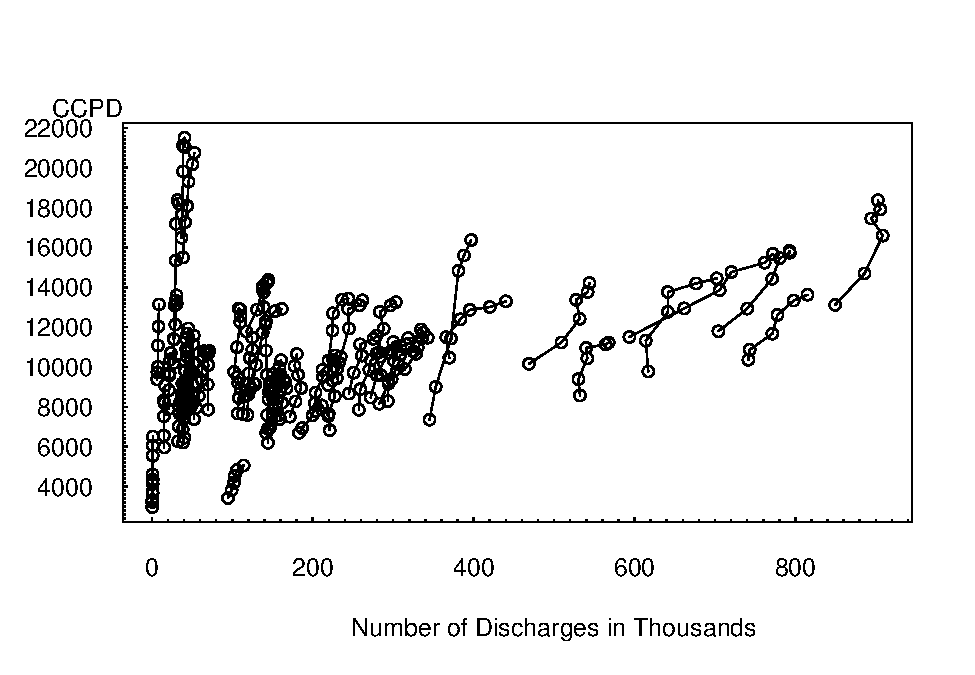
\includegraphics{LongPanelDataScripts_files/figure-latex/unnamed-chunk-17-1.pdf}

\hypertarget{figure-2.3-ccpd-vs-ave.days}{%
\subsection{Figure 2.3: CCPD vs AVE.DAYS}\label{figure-2.3-ccpd-vs-ave.days}}

Figure 2.3 is a scatter plot of CCPD versus average total days, connecting observations over time. This plot demonstrates the unusual nature of the second observation for the 54th state.

\begin{Shaded}
\begin{Highlighting}[]
\KeywordTok{plot}\NormalTok{(CCPD }\OperatorTok{~}\StringTok{ }\NormalTok{AVE.DAYS, }\DataTypeTok{data =}\NormalTok{ Medicare, }\DataTypeTok{ylab=}\StringTok{""}\NormalTok{, }\DataTypeTok{xlab=}\StringTok{""}\NormalTok{, }\DataTypeTok{xaxt=}\StringTok{"n"}\NormalTok{, }\DataTypeTok{yaxt=}\StringTok{"n"}\NormalTok{)}
\ControlFlowTok{for}\NormalTok{ (i }\ControlFlowTok{in}\NormalTok{ Medicare}\OperatorTok{$}\NormalTok{STATE) \{}
 \KeywordTok{lines}\NormalTok{(CCPD }\OperatorTok{~}\StringTok{ }\NormalTok{AVE.DAYS, }\DataTypeTok{data =} \KeywordTok{subset}\NormalTok{(Medicare, STATE}\OperatorTok{==}\StringTok{ }\NormalTok{i)) \}}
\KeywordTok{axis}\NormalTok{(}\DecValTok{2}\NormalTok{, }\DataTypeTok{at=}\KeywordTok{seq}\NormalTok{(}\DecValTok{0}\NormalTok{, }\DecValTok{22000}\NormalTok{, }\DataTypeTok{by=}\DecValTok{2000}\NormalTok{), }\DataTypeTok{las=}\DecValTok{1}\NormalTok{, }\DataTypeTok{font=}\DecValTok{10}\NormalTok{, }\DataTypeTok{cex=}\FloatTok{0.005}\NormalTok{, }\DataTypeTok{tck=}\FloatTok{0.01}\NormalTok{)}
\KeywordTok{axis}\NormalTok{(}\DecValTok{2}\NormalTok{, }\DataTypeTok{at=}\KeywordTok{seq}\NormalTok{(}\DecValTok{0}\NormalTok{, }\DecValTok{22000}\NormalTok{, }\DataTypeTok{by=}\DecValTok{200}\NormalTok{), }\DataTypeTok{lab=}\NormalTok{F, }\DataTypeTok{tck=}\FloatTok{0.005}\NormalTok{)}
\KeywordTok{axis}\NormalTok{(}\DecValTok{1}\NormalTok{, }\DataTypeTok{at=}\KeywordTok{seq}\NormalTok{(}\DecValTok{0}\NormalTok{,}\DecValTok{70}\NormalTok{, }\DataTypeTok{by=}\DecValTok{10}\NormalTok{), }\DataTypeTok{font=}\DecValTok{10}\NormalTok{, }\DataTypeTok{cex=}\FloatTok{0.005}\NormalTok{, }\DataTypeTok{tck=}\FloatTok{0.01}\NormalTok{)}
\KeywordTok{axis}\NormalTok{(}\DecValTok{1}\NormalTok{, }\DataTypeTok{at=}\KeywordTok{seq}\NormalTok{(}\DecValTok{0}\NormalTok{,}\DecValTok{70}\NormalTok{, }\DataTypeTok{by=}\DecValTok{1}\NormalTok{), }\DataTypeTok{lab=}\NormalTok{F, }\DataTypeTok{tck=}\FloatTok{0.005}\NormalTok{)}
\KeywordTok{mtext}\NormalTok{(}\StringTok{"CCPD"}\NormalTok{, }\DataTypeTok{side=}\DecValTok{2}\NormalTok{, }\DataTypeTok{line=}\DecValTok{0}\NormalTok{, }\DataTypeTok{at=}\DecValTok{23000}\NormalTok{, }\DataTypeTok{font=}\DecValTok{12}\NormalTok{, }\DataTypeTok{cex=}\DecValTok{1}\NormalTok{, }\DataTypeTok{las=}\DecValTok{1}\NormalTok{)}
\KeywordTok{mtext}\NormalTok{(}\StringTok{"Average Hospital Stay"}\NormalTok{, }\DataTypeTok{side=}\DecValTok{1}\NormalTok{, }\DataTypeTok{line=}\DecValTok{3}\NormalTok{, }\DataTypeTok{at=}\DecValTok{35}\NormalTok{, }\DataTypeTok{font=}\DecValTok{12}\NormalTok{, }\DataTypeTok{cex=}\DecValTok{1}\NormalTok{)}
\end{Highlighting}
\end{Shaded}

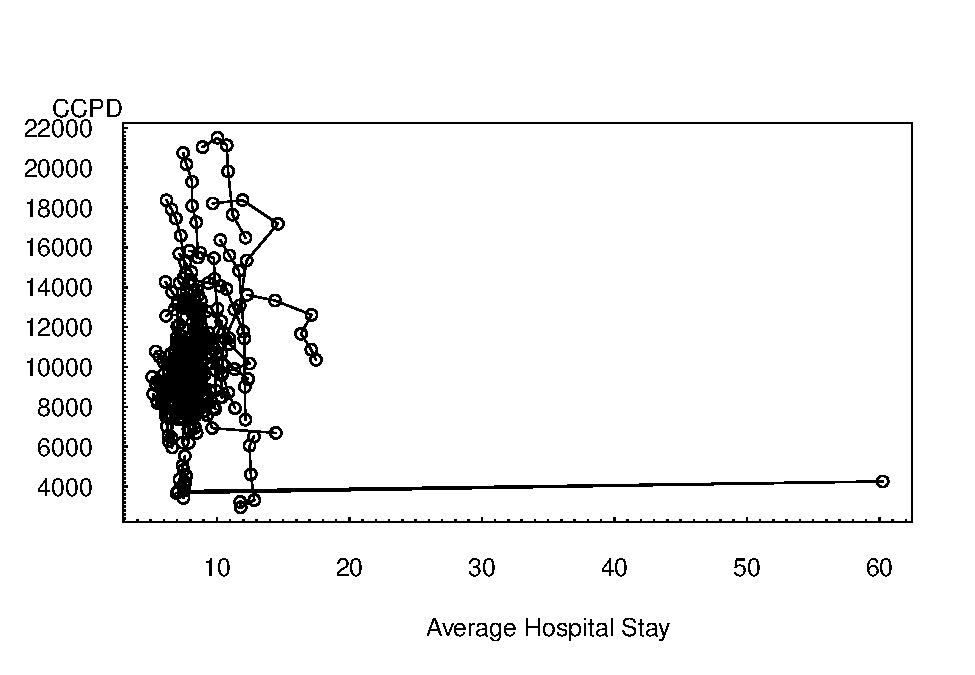
\includegraphics{LongPanelDataScripts_files/figure-latex/unnamed-chunk-18-1.pdf}

\hypertarget{figure-2.4-added-variable-plot-of-ccpd-versus-year}{%
\subsection{Figure 2.4: Added-variable plot of CCPD versus year}\label{figure-2.4-added-variable-plot-of-ccpd-versus-year}}

\begin{Shaded}
\begin{Highlighting}[]
\CommentTok{#  CREATE A CATEGORICAL VARIABLE for STATE;}
\NormalTok{Medicare}\OperatorTok{$}\NormalTok{FSTATE =}\StringTok{ }\KeywordTok{factor}\NormalTok{(Medicare}\OperatorTok{$}\NormalTok{STATE)}

\CommentTok{#  CREATE A NEW VARIABLE;}
\NormalTok{Medicare}\OperatorTok{$}\NormalTok{YEAR=Medicare}\OperatorTok{$}\NormalTok{YEAR}\DecValTok{-1989}
\CommentTok{# THE NEW VARIABLES YR31 WILL BE USED IN THE FINAL MODEL TO GIVE THE 31st STATE A SPECIFIC SLOPE;}
\NormalTok{Medicare}\OperatorTok{$}\NormalTok{Yr31=(Medicare}\OperatorTok{$}\NormalTok{STATE}\OperatorTok{==}\DecValTok{31}\NormalTok{)}\OperatorTok{*}\NormalTok{Medicare}\OperatorTok{$}\NormalTok{YEAR}

\CommentTok{#  CREATE A NEW DATA SET, REMOVING THE OUTLIER BY EXCLUDING THE 2ND OBSERVATION OF THE 54TH STATE;}
\NormalTok{Medicare2 =}\StringTok{ }\KeywordTok{subset}\NormalTok{(Medicare, STATE }\OperatorTok{!=}\StringTok{ }\DecValTok{54} \OperatorTok{|}\StringTok{ }\NormalTok{YEAR }\OperatorTok{!=}\StringTok{ }\DecValTok{2}\NormalTok{)}
\end{Highlighting}
\end{Shaded}

Figure 2.4 illustrates the basic added-variable plot. This plot portrays CCPD versus year, after excluding the second observation for the 54th state.

\begin{Shaded}
\begin{Highlighting}[]
\CommentTok{#  BASIC ADDED VARIABLE PLOT;}
\CommentTok{#  CREATE RESIDUALS;}
\NormalTok{Med1.lm =}\StringTok{ }\KeywordTok{lm}\NormalTok{(CCPD }\OperatorTok{~}\StringTok{ }\NormalTok{FSTATE, }\DataTypeTok{data=}\NormalTok{Medicare2)}
\NormalTok{Med2.lm =}\StringTok{ }\KeywordTok{lm}\NormalTok{(YEAR }\OperatorTok{~}\StringTok{ }\NormalTok{FSTATE, }\DataTypeTok{data=}\NormalTok{Medicare2)}
\NormalTok{Medicare2}\OperatorTok{$}\NormalTok{rCCPD=}\KeywordTok{residuals}\NormalTok{(Med1.lm)}
\NormalTok{Medicare2}\OperatorTok{$}\NormalTok{rYEAR=}\KeywordTok{residuals}\NormalTok{(Med2.lm)}
\KeywordTok{plot}\NormalTok{(rCCPD }\OperatorTok{~}\StringTok{ }\NormalTok{rYEAR, }\DataTypeTok{data=}\NormalTok{Medicare2, }\DataTypeTok{ylab=}\StringTok{""}\NormalTok{, }\DataTypeTok{xlab=}\StringTok{""}\NormalTok{, }\DataTypeTok{xaxt=}\StringTok{"n"}\NormalTok{, }\DataTypeTok{yaxt=}\StringTok{"n"}\NormalTok{)}
\ControlFlowTok{for}\NormalTok{ (i }\ControlFlowTok{in}\NormalTok{ Medicare2}\OperatorTok{$}\NormalTok{STATE) \{}
  \KeywordTok{lines}\NormalTok{(rCCPD }\OperatorTok{~}\StringTok{ }\NormalTok{rYEAR, }\DataTypeTok{data =} \KeywordTok{subset}\NormalTok{(Medicare2, STATE}\OperatorTok{==}\StringTok{ }\NormalTok{i)) \}}
\KeywordTok{axis}\NormalTok{(}\DecValTok{2}\NormalTok{, }\DataTypeTok{at=}\KeywordTok{seq}\NormalTok{(}\OperatorTok{-}\DecValTok{6000}\NormalTok{, }\DecValTok{4000}\NormalTok{, }\DataTypeTok{by=}\DecValTok{2000}\NormalTok{), }\DataTypeTok{las=}\DecValTok{1}\NormalTok{, }\DataTypeTok{font=}\DecValTok{10}\NormalTok{, }\DataTypeTok{cex=}\FloatTok{0.005}\NormalTok{, }\DataTypeTok{tck=}\FloatTok{0.01}\NormalTok{)}
\KeywordTok{axis}\NormalTok{(}\DecValTok{2}\NormalTok{, }\DataTypeTok{at=}\KeywordTok{seq}\NormalTok{(}\OperatorTok{-}\DecValTok{6000}\NormalTok{, }\DecValTok{4000}\NormalTok{, }\DataTypeTok{by=}\DecValTok{200}\NormalTok{), }\DataTypeTok{lab=}\NormalTok{F, }\DataTypeTok{tck=}\FloatTok{0.005}\NormalTok{)}
\KeywordTok{axis}\NormalTok{(}\DecValTok{1}\NormalTok{, }\DataTypeTok{at=}\KeywordTok{seq}\NormalTok{(}\OperatorTok{-}\DecValTok{3}\NormalTok{,}\DecValTok{3}\NormalTok{, }\DataTypeTok{by=}\DecValTok{1}\NormalTok{), }\DataTypeTok{font=}\DecValTok{10}\NormalTok{, }\DataTypeTok{cex=}\FloatTok{0.005}\NormalTok{, }\DataTypeTok{tck=}\FloatTok{0.01}\NormalTok{)}
\KeywordTok{axis}\NormalTok{(}\DecValTok{1}\NormalTok{, }\DataTypeTok{at=}\KeywordTok{seq}\NormalTok{(}\OperatorTok{-}\DecValTok{3}\NormalTok{,}\DecValTok{3}\NormalTok{, }\DataTypeTok{by=}\FloatTok{0.1}\NormalTok{), }\DataTypeTok{lab=}\NormalTok{F, }\DataTypeTok{tck=}\FloatTok{0.005}\NormalTok{)}
\KeywordTok{mtext}\NormalTok{(}\StringTok{"Residuals from CCPD"}\NormalTok{, }\DataTypeTok{side=}\DecValTok{2}\NormalTok{, }\DataTypeTok{line=}\OperatorTok{-}\DecValTok{8}\NormalTok{, }\DataTypeTok{at=}\DecValTok{5000}\NormalTok{, }\DataTypeTok{font=}\DecValTok{12}\NormalTok{, }\DataTypeTok{cex=}\DecValTok{1}\NormalTok{, }\DataTypeTok{las=}\DecValTok{1}\NormalTok{)}
\KeywordTok{mtext}\NormalTok{(}\StringTok{"Residuals from YEAR"}\NormalTok{, }\DataTypeTok{side=}\DecValTok{1}\NormalTok{, }\DataTypeTok{line=}\DecValTok{3}\NormalTok{, }\DataTypeTok{at=}\DecValTok{0}\NormalTok{, }\DataTypeTok{font=}\DecValTok{12}\NormalTok{, }\DataTypeTok{cex=}\DecValTok{1}\NormalTok{)}
\end{Highlighting}
\end{Shaded}

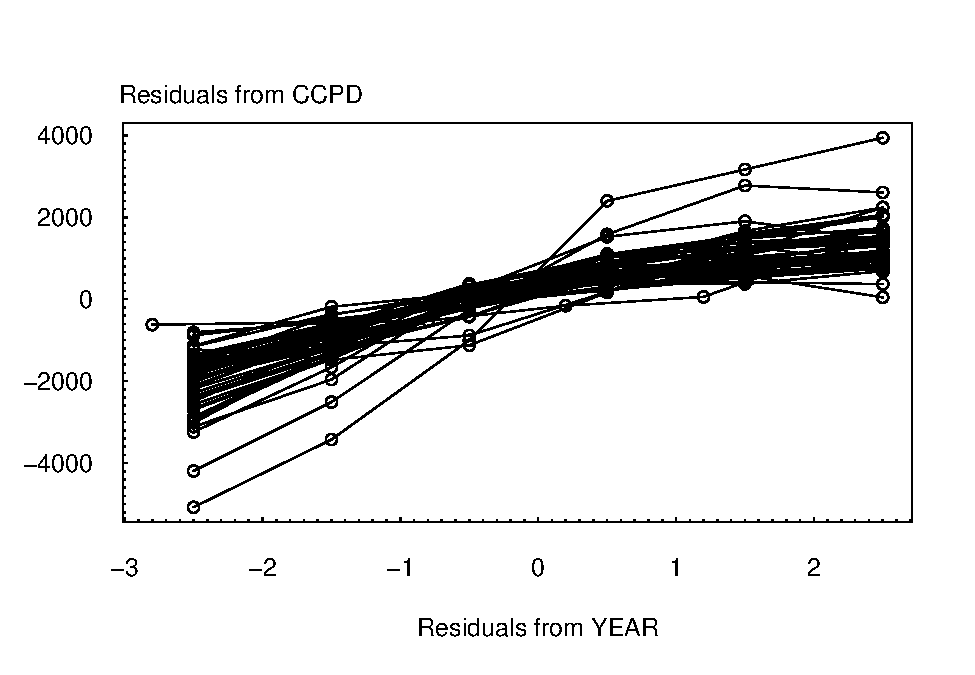
\includegraphics{LongPanelDataScripts_files/figure-latex/unnamed-chunk-20-1.pdf}

\hypertarget{figure-2.5-trellis-plot}{%
\subsection{Figure 2.5: Trellis Plot}\label{figure-2.5-trellis-plot}}

A technique for graphical display that has recently become popular in the statistical literature is a trellis plot. This graphical technique takes its name from a trellis, which is a structure of open latticework.
Figure 2.5 illustrates the use of small multiples. In each panel, the plot portrayed is identical except that it is based on a different state; this use of
parallel structure allows us to demonstrate the increasing CCPD for each state.

\begin{Shaded}
\begin{Highlighting}[]
\NormalTok{GrpMedicare =}\StringTok{ }\KeywordTok{groupedData}\NormalTok{(CCPD }\OperatorTok{~}\StringTok{ }\NormalTok{YEAR}\OperatorTok{|}\StringTok{ }\NormalTok{NMSTATE, }\DataTypeTok{data=}\NormalTok{Medicare2)}
\KeywordTok{plot}\NormalTok{(GrpMedicare, }\DataTypeTok{xlab=}\StringTok{"YEAR"}\NormalTok{, }\DataTypeTok{ylab=}\StringTok{"CCPD"}\NormalTok{, }\DataTypeTok{scale =} \KeywordTok{list}\NormalTok{(}\DataTypeTok{x=}\KeywordTok{list}\NormalTok{(}\DataTypeTok{draw=}\OtherTok{FALSE}\NormalTok{)), }\DataTypeTok{layout=}\KeywordTok{c}\NormalTok{(}\DecValTok{18}\NormalTok{,}\DecValTok{3}\NormalTok{))}
\end{Highlighting}
\end{Shaded}

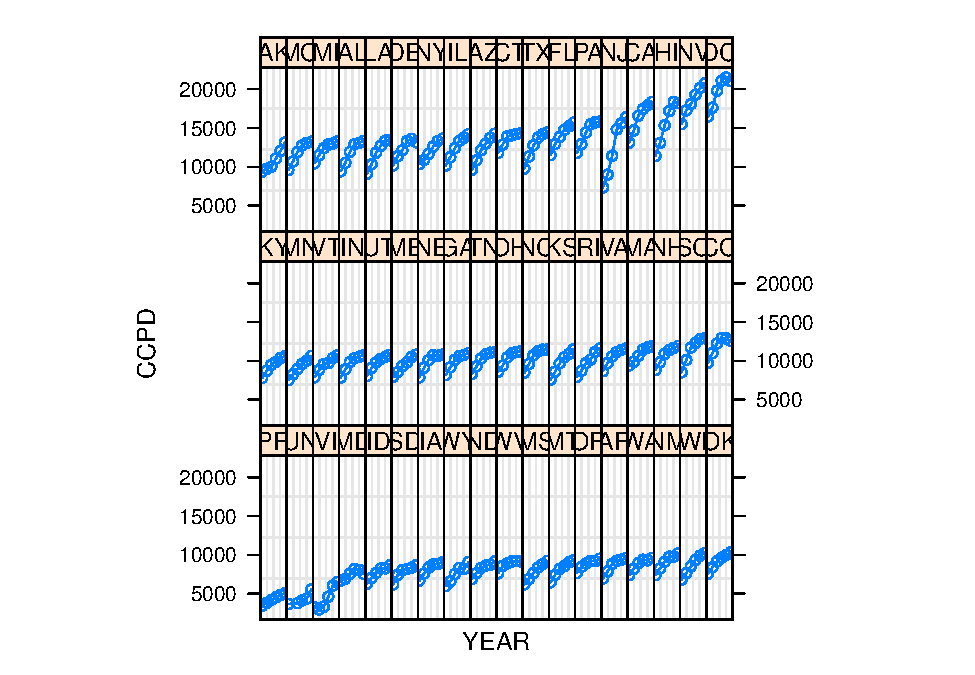
\includegraphics{LongPanelDataScripts_files/figure-latex/unnamed-chunk-21-1.pdf}

\hypertarget{one-way-fixed-effects-model-using-lm-for-linear-model}{%
\section{One way fixed effects model using lm, for linear model}\label{one-way-fixed-effects-model-using-lm-for-linear-model}}

See Example 2.2: Medicare Hospital Costs.

\begin{Shaded}
\begin{Highlighting}[]
\NormalTok{Medicare.lm =}\StringTok{ }\KeywordTok{lm}\NormalTok{(CCPD }\OperatorTok{~}\StringTok{ }\NormalTok{NUM.DCHG }\OperatorTok{+}\StringTok{ }\NormalTok{Yr31 }\OperatorTok{+}\StringTok{ }\NormalTok{YEAR }\OperatorTok{+}\StringTok{ }\NormalTok{AVE.DAYS }\OperatorTok{+}\StringTok{ }\NormalTok{FSTATE }\OperatorTok{-}\StringTok{ }\DecValTok{1}\NormalTok{, }\DataTypeTok{data=}\NormalTok{Medicare2)}
\KeywordTok{summary}\NormalTok{(Medicare.lm)}
\end{Highlighting}
\end{Shaded}

\begin{verbatim}

Call:
lm(formula = CCPD ~ NUM.DCHG + Yr31 + YEAR + AVE.DAYS + FSTATE - 
    1, data = Medicare2)

Residuals:
     Min       1Q   Median       3Q      Max 
-1952.54  -264.66    50.46   300.10  1638.39 

Coefficients:
          Estimate Std. Error t value Pr(>|t|)    
NUM.DCHG    10.755      2.573   4.180 3.96e-05 ***
Yr31      1262.456    128.609   9.816  < 2e-16 ***
YEAR       710.884     26.812  26.513  < 2e-16 ***
AVE.DAYS   361.290     57.979   6.231 1.81e-09 ***
FSTATE1   3888.845    894.076   4.350 1.95e-05 ***
FSTATE2   5694.017    534.048  10.662  < 2e-16 ***
FSTATE3   5736.793    661.153   8.677 4.19e-16 ***
FSTATE4   1639.697    726.577   2.257  0.02484 *  
FSTATE5   1745.883   2402.770   0.727  0.46810    
FSTATE6   5519.532    639.097   8.636 5.52e-16 ***
FSTATE7   5882.663    815.649   7.212 5.77e-12 ***
FSTATE8   6319.729    625.690  10.100  < 2e-16 ***
FSTATE9  12842.939    733.122  17.518  < 2e-16 ***
FSTATE10   990.386   1962.480   0.505  0.61422    
FSTATE11  1352.055   1020.337   1.325  0.18628    
FSTATE12  8524.447    790.980  10.777  < 2e-16 ***
FSTATE13  2700.653    475.750   5.677 3.60e-08 ***
FSTATE14  1417.162   1526.064   0.929  0.35392    
FSTATE15  1383.831    952.843   1.452  0.14760    
FSTATE16  1426.408    696.791   2.047  0.04163 *  
FSTATE17  3146.952    673.351   4.674 4.72e-06 ***
FSTATE18  1728.006    844.017   2.047  0.04161 *  
FSTATE19  3926.979    867.993   4.524 9.16e-06 ***
FSTATE20  3242.727    639.799   5.068 7.54e-07 ***
FSTATE21  -711.562    898.191  -0.792  0.42894    
FSTATE22  1079.195   1161.922   0.929  0.35384    
FSTATE23  2480.023   1236.826   2.005  0.04596 *  
FSTATE24  2293.256    719.640   3.187  0.00161 ** 
FSTATE25   957.334    712.831   1.343  0.18042    
FSTATE26  3299.585    998.712   3.304  0.00109 ** 
FSTATE27  3003.060    494.942   6.068 4.47e-09 ***
FSTATE28  3755.028    615.706   6.099 3.77e-09 ***
FSTATE29 12615.456    598.073  21.094  < 2e-16 ***
FSTATE30  4401.868    669.931   6.571 2.64e-10 ***
FSTATE31 -2649.456   1345.138  -1.970  0.04992 *  
FSTATE32  3589.638    535.271   6.706 1.20e-10 ***
FSTATE33 -4444.768   2367.411  -1.877  0.06155 .  
FSTATE34  1354.039   1071.140   1.264  0.20730    
FSTATE35  2683.031    552.483   4.856 2.05e-06 ***
FSTATE36  -998.648   1578.677  -0.633  0.52755    
FSTATE37  2109.789    736.174   2.866  0.00449 ** 
FSTATE38  3082.538    552.317   5.581 5.90e-08 ***
FSTATE39   260.811   2145.305   0.122  0.90333    
FSTATE40 -2006.729    631.691  -3.177  0.00167 ** 
FSTATE41  2978.161    744.200   4.002 8.16e-05 ***
FSTATE42  3819.468    803.495   4.754 3.28e-06 ***
FSTATE43  2398.622    532.257   4.507 9.90e-06 ***
FSTATE44  1498.689   1017.547   1.473  0.14198    
FSTATE45   277.739   1831.029   0.152  0.87955    
FSTATE46  4580.418    496.141   9.232  < 2e-16 ***
FSTATE47  3612.284    621.289   5.814 1.75e-08 ***
FSTATE48 -2516.614    807.777  -3.115  0.00204 ** 
FSTATE49  2213.600    943.221   2.347  0.01967 *  
FSTATE50  2138.158    685.695   3.118  0.00202 ** 
FSTATE51  2101.881    677.712   3.101  0.00213 ** 
FSTATE52  1138.089    835.624   1.362  0.17437    
FSTATE53  2784.381    471.058   5.911 1.04e-08 ***
FSTATE54 -1037.318    544.265  -1.906  0.05774 .  
---
Signif. codes:  0 '***' 0.001 '**' 0.01 '*' 0.05 '.' 0.1 ' ' 1

Residual standard error: 529.5 on 265 degrees of freedom
Multiple R-squared:  0.9981,    Adjusted R-squared:  0.9977 
F-statistic:  2392 on 58 and 265 DF,  p-value: < 2.2e-16
\end{verbatim}

\begin{Shaded}
\begin{Highlighting}[]
\KeywordTok{anova}\NormalTok{(Medicare.lm)}
\end{Highlighting}
\end{Shaded}

\begin{verbatim}
Analysis of Variance Table

Response: CCPD
           Df     Sum Sq    Mean Sq  F value    Pr(>F)    
NUM.DCHG    1 2.1693e+10 2.1693e+10 77387.47 < 2.2e-16 ***
Yr31        1 6.8708e+07 6.8708e+07   245.11 < 2.2e-16 ***
YEAR        1 1.1974e+10 1.1974e+10 42716.19 < 2.2e-16 ***
AVE.DAYS    1 2.6659e+09 2.6659e+09  9510.30 < 2.2e-16 ***
FSTATE     54 2.4833e+09 4.5986e+07   164.05 < 2.2e-16 ***
Residuals 265 7.4284e+07 2.8032e+05                       
---
Signif. codes:  0 '***' 0.001 '**' 0.01 '*' 0.05 '.' 0.1 ' ' 1
\end{verbatim}

\hypertarget{section-2.4.1---analysis-for-the-pooling-test}{%
\section{SECTION 2.4.1 - Analysis for the pooling test;}\label{section-2.4.1---analysis-for-the-pooling-test}}

We can check the F-ratio by \texttt{anova(Medicare.lm,Medicare3.lm)}. We reject the null hypothesis from the result below.

\begin{Shaded}
\begin{Highlighting}[]
\NormalTok{Medicare3.lm =}\StringTok{ }\KeywordTok{lm}\NormalTok{(CCPD }\OperatorTok{~}\StringTok{ }\NormalTok{NUM.DCHG}\OperatorTok{+}\StringTok{ }\NormalTok{Yr31 }\OperatorTok{+}\StringTok{ }\NormalTok{YEAR }\OperatorTok{+}\StringTok{ }\NormalTok{AVE.DAYS , }\DataTypeTok{data=}\NormalTok{Medicare2)}
\KeywordTok{summary}\NormalTok{(Medicare3.lm)}
\end{Highlighting}
\end{Shaded}

\begin{verbatim}

Call:
lm(formula = CCPD ~ NUM.DCHG + Yr31 + YEAR + AVE.DAYS, data = Medicare2)

Residuals:
    Min      1Q  Median      3Q     Max 
-7176.7 -1255.3  -384.9  1092.4 10350.9 

Coefficients:
             Estimate Std. Error t value Pr(>|t|)    
(Intercept) 4342.1049   873.4212   4.971 1.09e-06 ***
NUM.DCHG       4.6606     0.7241   6.436 4.51e-10 ***
Yr31         299.9270   295.8341   1.014 0.311432    
YEAR         733.2750    94.1398   7.789 9.62e-14 ***
AVE.DAYS     308.4710    86.0766   3.584 0.000392 ***
---
Signif. codes:  0 '***' 0.001 '**' 0.01 '*' 0.05 '.' 0.1 ' ' 1

Residual standard error: 2732 on 318 degrees of freedom
Multiple R-squared:  0.2879,    Adjusted R-squared:  0.279 
F-statistic: 32.15 on 4 and 318 DF,  p-value: < 2.2e-16
\end{verbatim}

\begin{Shaded}
\begin{Highlighting}[]
\KeywordTok{anova}\NormalTok{(Medicare3.lm)}
\end{Highlighting}
\end{Shaded}

\begin{verbatim}
Analysis of Variance Table

Response: CCPD
           Df     Sum Sq   Mean Sq F value    Pr(>F)    
NUM.DCHG    1  463168764 463168764 62.0651 5.317e-14 ***
Yr31        1   33908652  33908652  4.5438 0.0338046 *  
YEAR        1  366756374 366756374 49.1457 1.430e-11 ***
AVE.DAYS    1   95840842  95840842 12.8428 0.0003919 ***
Residuals 318 2373115933   7462629                      
---
Signif. codes:  0 '***' 0.001 '**' 0.01 '*' 0.05 '.' 0.1 ' ' 1
\end{verbatim}

\begin{Shaded}
\begin{Highlighting}[]
\KeywordTok{anova}\NormalTok{(Medicare3.lm,Medicare.lm) }\CommentTok{# pooling test}
\end{Highlighting}
\end{Shaded}

\begin{verbatim}
Analysis of Variance Table

Model 1: CCPD ~ NUM.DCHG + Yr31 + YEAR + AVE.DAYS
Model 2: CCPD ~ NUM.DCHG + Yr31 + YEAR + AVE.DAYS + FSTATE - 1
  Res.Df        RSS Df  Sum of Sq      F    Pr(>F)    
1    318 2373115933                                   
2    265   74284379 53 2298831554 154.73 < 2.2e-16 ***
---
Signif. codes:  0 '***' 0.001 '**' 0.01 '*' 0.05 '.' 0.1 ' ' 1
\end{verbatim}

\hypertarget{section-2.4.2---correlation-corresponding-to-the-added-variable-plot}{%
\section{SECTION 2.4.2 - Correlation corresponding to the added variable plot;}\label{section-2.4.2---correlation-corresponding-to-the-added-variable-plot}}

As with all scatter plots, the added-variable plot can be summarized numerically through a correlation coefficient that we will denote by \(corr(e_1, e_2)\).

\begin{Shaded}
\begin{Highlighting}[]
\CommentTok{#  SECTION 2.4.2 - CORRELATION CORRESPONDING TO THE ADDED VARIABLE PLOT;}
\KeywordTok{library}\NormalTok{(boot)}
\KeywordTok{cor}\NormalTok{(Medicare2}\OperatorTok{$}\NormalTok{rCCPD , Medicare2}\OperatorTok{$}\NormalTok{rYEAR)}
\end{Highlighting}
\end{Shaded}

\begin{verbatim}
[1] 0.8847151
\end{verbatim}

\hypertarget{section-2.4.5---testing-for-heteroscedasticity}{%
\section{SECTION 2.4.5 - Testing for heteroscedasticity;}\label{section-2.4.5---testing-for-heteroscedasticity}}

When fitting regression models to data, an important assumption is that the variability is common among all observations. This assumption of common variability is called homoscedasticity, meaning ``same scatter''.

\begin{Shaded}
\begin{Highlighting}[]
\NormalTok{Medicare2}\OperatorTok{$}\NormalTok{Resids=}\KeywordTok{residuals}\NormalTok{(Medicare.lm)}
\NormalTok{Medicare2}\OperatorTok{$}\NormalTok{ResidSq=Medicare2}\OperatorTok{$}\NormalTok{Resids}\OperatorTok{*}\NormalTok{Medicare2}\OperatorTok{$}\NormalTok{Resids}
\NormalTok{MedHet.lm =}\StringTok{ }\KeywordTok{lm}\NormalTok{(ResidSq }\OperatorTok{~}\StringTok{ }\NormalTok{NUM.DCHG, }\DataTypeTok{data=}\NormalTok{Medicare2)}
\KeywordTok{summary}\NormalTok{(MedHet.lm)}
\end{Highlighting}
\end{Shaded}

\begin{verbatim}

Call:
lm(formula = ResidSq ~ NUM.DCHG, data = Medicare2)

Residuals:
    Min      1Q  Median      3Q     Max 
-255383 -212155 -143167    7752 3555249 

Coefficients:
            Estimate Std. Error t value Pr(>|t|)    
(Intercept) 261171.0    35324.5   7.393 1.25e-12 ***
NUM.DCHG      -147.5      116.8  -1.264    0.207    
---
Signif. codes:  0 '***' 0.001 '**' 0.01 '*' 0.05 '.' 0.1 ' ' 1

Residual standard error: 454200 on 321 degrees of freedom
Multiple R-squared:  0.004949,  Adjusted R-squared:  0.001849 
F-statistic: 1.597 on 1 and 321 DF,  p-value: 0.2073
\end{verbatim}

\begin{Shaded}
\begin{Highlighting}[]
\KeywordTok{anova}\NormalTok{(MedHet.lm)}
\end{Highlighting}
\end{Shaded}

\begin{verbatim}
Analysis of Variance Table

Response: ResidSq
           Df     Sum Sq    Mean Sq F value Pr(>F)
NUM.DCHG    1 3.2930e+11 3.2930e+11  1.5966 0.2073
Residuals 321 6.6208e+13 2.0625e+11               
\end{verbatim}

\hypertarget{one-way-random-effects-model-using-lm-for-linear-model}{%
\subsection{One way random effects model using lm, for linear model;}\label{one-way-random-effects-model-using-lm-for-linear-model}}

We will learn random effects model in Chapter 3. Here is an example.

\begin{Shaded}
\begin{Highlighting}[]
\NormalTok{Medicare.lme =}\StringTok{ }\KeywordTok{lme}\NormalTok{(CCPD }\OperatorTok{~}\StringTok{ }\NormalTok{NUM.DCHG, }\DataTypeTok{data=}\NormalTok{Medicare2, }\DataTypeTok{random =} \OperatorTok{~}\DecValTok{1}\OperatorTok{|}\NormalTok{STATE)}
\KeywordTok{summary}\NormalTok{(Medicare.lme)}
\end{Highlighting}
\end{Shaded}

\begin{verbatim}
Linear mixed-effects model fit by REML
 Data: Medicare2 
       AIC      BIC    logLik
  5733.495 5748.581 -2862.747

Random effects:
 Formula: ~1 | STATE
        (Intercept) Residual
StdDev:    3016.201 1316.346

Fixed effects: CCPD ~ NUM.DCHG 
               Value Std.Error  DF   t-value p-value
(Intercept) 8084.128  564.3211 268 14.325404       0
NUM.DCHG      11.386    1.8044 268  6.310388       0
 Correlation: 
         (Intr)
NUM.DCHG -0.674

Standardized Within-Group Residuals:
       Min         Q1        Med         Q3        Max 
-3.6167201 -0.6276783  0.1998388  0.6325460  2.7846480 

Number of Observations: 323
Number of Groups: 54 
\end{verbatim}

\hypertarget{models-with-random-effects}{%
\chapter{Models with Random Effects}\label{models-with-random-effects}}

\hypertarget{import-data-2}{%
\section{Import Data}\label{import-data-2}}

\begin{Shaded}
\begin{Highlighting}[]
\CommentTok{#  "\textbackslash{}t"  INDICATES SEPARATED BY TABLES  ;}
\NormalTok{taxprep  =}\StringTok{ }\KeywordTok{read.table}\NormalTok{(}\StringTok{"TXTData/TaxPrep.txt"}\NormalTok{, }\DataTypeTok{sep =}\StringTok{"}\CharTok{\textbackslash{}t}\StringTok{"}\NormalTok{, }\DataTypeTok{quote =} \StringTok{""}\NormalTok{,}\DataTypeTok{header=}\OtherTok{TRUE}\NormalTok{)}

\CommentTok{# taxprep=read.table(choose.files(), header=TRUE, sep="\textbackslash{}t")}
\end{Highlighting}
\end{Shaded}

Data for this study are from the Statistics of Income (SOI) Panel of Individual Returns, a part of the Ernst and Young/University of Michigan Tax Research Database. The SOI Panel represents a simple random sample of unaudited individual income tax returns filed for tax years 1979-1990. The data are compiled from a stratified probability sample of unaudited individual income tax returns, Forms 1040, 1040A and 1040EZ, filed by U.S. taxpayers. The estimates that are obtained from these data are intended to represent all returns filed for the income tax years under review. All returns processed are subjected to sampling except tentative and amended returns.

\begin{longtable}[]{@{}ll@{}}
\toprule
\begin{minipage}[b]{0.06\columnwidth}\raggedright
Variable\strut
\end{minipage} & \begin{minipage}[b]{0.88\columnwidth}\raggedright
Description\strut
\end{minipage}\tabularnewline
\midrule
\endhead
\begin{minipage}[t]{0.06\columnwidth}\raggedright
MS\strut
\end{minipage} & \begin{minipage}[t]{0.88\columnwidth}\raggedright
is an indicator variable of the taxpayer's marital status. It is coded one if the taxpayer is married and zero otherwise.\strut
\end{minipage}\tabularnewline
\begin{minipage}[t]{0.06\columnwidth}\raggedright
HH\strut
\end{minipage} & \begin{minipage}[t]{0.88\columnwidth}\raggedright
is an indicator variable, one if the taxpayer is a head of household and zero otherwise.\strut
\end{minipage}\tabularnewline
\begin{minipage}[t]{0.06\columnwidth}\raggedright
DEPEND\strut
\end{minipage} & \begin{minipage}[t]{0.88\columnwidth}\raggedright
is the number of dependents claimed by the taxpayer.\strut
\end{minipage}\tabularnewline
\begin{minipage}[t]{0.06\columnwidth}\raggedright
AGE\strut
\end{minipage} & \begin{minipage}[t]{0.88\columnwidth}\raggedright
is the presence of an indicator for age 65 or over.\strut
\end{minipage}\tabularnewline
\begin{minipage}[t]{0.06\columnwidth}\raggedright
F1040A\strut
\end{minipage} & \begin{minipage}[t]{0.88\columnwidth}\raggedright
is an indicator variable of the taxpayer's filing type. It is coded one if the taxpayer uses Form 1040A and zero otherwise.\strut
\end{minipage}\tabularnewline
\begin{minipage}[t]{0.06\columnwidth}\raggedright
F1040EZ\strut
\end{minipage} & \begin{minipage}[t]{0.88\columnwidth}\raggedright
is an indicator variable of the taxpayer's filing type. It is coded one if the taxpayer uses Form 1040EZ and zero otherwise.\strut
\end{minipage}\tabularnewline
\begin{minipage}[t]{0.06\columnwidth}\raggedright
TPI\strut
\end{minipage} & \begin{minipage}[t]{0.88\columnwidth}\raggedright
is the sum of all positive income line items on the return. is a marginal tax rate.\strut
\end{minipage}\tabularnewline
\begin{minipage}[t]{0.06\columnwidth}\raggedright
TXRT\strut
\end{minipage} & \begin{minipage}[t]{0.88\columnwidth}\raggedright
is a marginal tax rate。 It is computed on TPI less exemptions and the standard deduction.\strut
\end{minipage}\tabularnewline
\begin{minipage}[t]{0.06\columnwidth}\raggedright
MR\strut
\end{minipage} & \begin{minipage}[t]{0.88\columnwidth}\raggedright
is an exogenous marginal tax rate. It is computed on TPI less exemptions and the standard deduction.\strut
\end{minipage}\tabularnewline
\begin{minipage}[t]{0.06\columnwidth}\raggedright
EMP\strut
\end{minipage} & \begin{minipage}[t]{0.88\columnwidth}\raggedright
is an indicator variable, one if Schedule C or F is present and zero otherwise. Self-employed taxpayers have greater need for professional assistance to reduce the reporting risks of doing business.\strut
\end{minipage}\tabularnewline
\begin{minipage}[t]{0.06\columnwidth}\raggedright
PREP\strut
\end{minipage} & \begin{minipage}[t]{0.88\columnwidth}\raggedright
is a variable indicating the presence of a paid preparer.\strut
\end{minipage}\tabularnewline
\begin{minipage}[t]{0.06\columnwidth}\raggedright
TAX\strut
\end{minipage} & \begin{minipage}[t]{0.88\columnwidth}\raggedright
is the tax liability on the return.\strut
\end{minipage}\tabularnewline
\begin{minipage}[t]{0.06\columnwidth}\raggedright
SUBJECT\strut
\end{minipage} & \begin{minipage}[t]{0.88\columnwidth}\raggedright
Subject identifier, 1- 258.\strut
\end{minipage}\tabularnewline
\begin{minipage}[t]{0.06\columnwidth}\raggedright
TIME\strut
\end{minipage} & \begin{minipage}[t]{0.88\columnwidth}\raggedright
Time identifier, 1-5.\strut
\end{minipage}\tabularnewline
\begin{minipage}[t]{0.06\columnwidth}\raggedright
LNTAX\strut
\end{minipage} & \begin{minipage}[t]{0.88\columnwidth}\raggedright
is the natural logarithm of the tax liability on the return.\strut
\end{minipage}\tabularnewline
\begin{minipage}[t]{0.06\columnwidth}\raggedright
LNTPI\strut
\end{minipage} & \begin{minipage}[t]{0.88\columnwidth}\raggedright
is the natural logarithm of the sum of all positive income line items on the return.\strut
\end{minipage}\tabularnewline
\bottomrule
\end{longtable}

\hypertarget{example-3.2-income-tax-payments-page-81}{%
\section{Example 3.2: Income Tax Payments (Page 81)}\label{example-3.2-income-tax-payments-page-81}}

In this section, we study the effects that an individual's economic and demographic characteristics have on the amount of income tax paid. Specifically, the response of interest is \texttt{LNTAX}, defined as the natural logarithm of the liability on the tax return.

\hypertarget{table-3.2.-averages-of-binary-variables}{%
\subsection{Table 3.2. Averages of binary variables}\label{table-3.2.-averages-of-binary-variables}}

The binary variables in Table 3.2 indicate that over half the sample is married (MS) and approximately half the sample uses a paid preparer (PREP).

\begin{Shaded}
\begin{Highlighting}[]
\KeywordTok{library}\NormalTok{(nlme)}
\KeywordTok{gsummary}\NormalTok{(taxprep[, }\KeywordTok{c}\NormalTok{(}\StringTok{"MS"}\NormalTok{, }\StringTok{"HH"}\NormalTok{, }\StringTok{"AGE"}\NormalTok{, }\StringTok{"EMP"}\NormalTok{, }\StringTok{"PREP"}\NormalTok{)], }\DataTypeTok{groups=}\NormalTok{taxprep}\OperatorTok{$}\NormalTok{TIME, }\DataTypeTok{FUN=}\NormalTok{mean)}
\end{Highlighting}
\end{Shaded}

\begin{verbatim}
         MS         HH        AGE       EMP      PREP
1 0.5968992 0.08139535 0.08527132 0.1395349 0.4496124
2 0.5968992 0.09302326 0.10465116 0.1589147 0.4418605
3 0.6240310 0.08527132 0.11240310 0.1550388 0.4844961
4 0.6472868 0.08139535 0.13178295 0.1472868 0.5077519
5 0.6472868 0.09302326 0.14728682 0.1472868 0.5155039
\end{verbatim}

\hypertarget{table-3.3---summary-statistics-for-continuous-variables}{%
\subsection{TABLE 3.3 - Summary statistics for continuous variables}\label{table-3.3---summary-statistics-for-continuous-variables}}

Tables 3.2 and 3.3 describe the basic taxpayer characteristics used in our analysis. The summary statistics for the other nonbinary variables are in Table 3.3.

\begin{Shaded}
\begin{Highlighting}[]
\KeywordTok{summary}\NormalTok{(taxprep[, }\KeywordTok{c}\NormalTok{(}\StringTok{"DEPEND"}\NormalTok{, }\StringTok{"LNTPI"}\NormalTok{, }\StringTok{"MR"}\NormalTok{, }\StringTok{"LNTAX"}\NormalTok{)]) }\CommentTok{#summary does not provid standard deviation}
\end{Highlighting}
\end{Shaded}

\begin{verbatim}
     DEPEND          LNTPI               MR            LNTAX       
 Min.   :0.000   Min.   :-0.1275   Min.   : 0.00   Min.   : 0.000  
 1st Qu.:1.000   1st Qu.: 9.4467   1st Qu.:15.00   1st Qu.: 6.645  
 Median :2.000   Median :10.0506   Median :22.00   Median : 7.701  
 Mean   :2.419   Mean   : 9.8886   Mean   :23.52   Mean   : 6.880  
 3rd Qu.:3.000   3rd Qu.:10.5320   3rd Qu.:33.00   3rd Qu.: 8.420  
 Max.   :6.000   Max.   :13.2220   Max.   :50.00   Max.   :11.860  
\end{verbatim}

Standard deviation of some variables.

\begin{Shaded}
\begin{Highlighting}[]
\CommentTok{#Standard Deviation}
\NormalTok{var<-}\KeywordTok{var}\NormalTok{(taxprep[, }\KeywordTok{c}\NormalTok{(}\StringTok{"DEPEND"}\NormalTok{, }\StringTok{"LNTPI"}\NormalTok{, }\StringTok{"MR"}\NormalTok{, }\StringTok{"LNTAX"}\NormalTok{)])}
\KeywordTok{sqrt}\NormalTok{(}\KeywordTok{diag}\NormalTok{(var))}
\end{Highlighting}
\end{Shaded}

\begin{verbatim}
   DEPEND     LNTPI        MR     LNTAX 
 1.337562  1.164625 11.453800  2.694961 
\end{verbatim}

\hypertarget{table-3.4---averages-by-level-of-binary-explanatory-variable}{%
\subsection{TABLE 3.4 - Averages by level of binary explanatory variable}\label{table-3.4---averages-by-level-of-binary-explanatory-variable}}

To explore the relationship between each indicator variable and logarithmic tax, Table 3.4 presents the average logarithmic tax liability by level of indicator variable. This table shows that married filers pay greater tax, head-of-household filers pay less tax, taxpayers 65 or over pay less, taxpayers with self-employed income pay less, and taxpayers who use a professional tax preparer pay more.

\begin{Shaded}
\begin{Highlighting}[]
\KeywordTok{library}\NormalTok{(Hmisc)}
\KeywordTok{summarize}\NormalTok{(taxprep}\OperatorTok{$}\NormalTok{LNTAX, taxprep}\OperatorTok{$}\NormalTok{MS, mean) }
\end{Highlighting}
\end{Shaded}

\begin{verbatim}
  taxprep$MS taxprep$LNTAX
1          0      5.973412
2          1      7.429948
\end{verbatim}

\begin{Shaded}
\begin{Highlighting}[]
\KeywordTok{summarize}\NormalTok{(taxprep}\OperatorTok{$}\NormalTok{LNTAX, taxprep}\OperatorTok{$}\NormalTok{HH, mean)}
\end{Highlighting}
\end{Shaded}

\begin{verbatim}
  taxprep$HH taxprep$LNTAX
1          0      7.013197
2          1      5.479947
\end{verbatim}

\begin{Shaded}
\begin{Highlighting}[]
\KeywordTok{summarize}\NormalTok{(taxprep}\OperatorTok{$}\NormalTok{LNTAX, taxprep}\OperatorTok{$}\NormalTok{AGE, mean)}
\end{Highlighting}
\end{Shaded}

\begin{verbatim}
  taxprep$AGE taxprep$LNTAX
1           0      6.939184
2           1      6.430867
\end{verbatim}

\begin{Shaded}
\begin{Highlighting}[]
\KeywordTok{summarize}\NormalTok{(taxprep}\OperatorTok{$}\NormalTok{LNTAX, taxprep}\OperatorTok{$}\NormalTok{EMP, mean)}
\end{Highlighting}
\end{Shaded}

\begin{verbatim}
  taxprep$EMP taxprep$LNTAX
1           0      6.982682
2           1      6.296879
\end{verbatim}

\begin{Shaded}
\begin{Highlighting}[]
\KeywordTok{summarize}\NormalTok{(taxprep}\OperatorTok{$}\NormalTok{LNTAX, taxprep}\OperatorTok{$}\NormalTok{PREP, mean)}
\end{Highlighting}
\end{Shaded}

\begin{verbatim}
  taxprep$PREP taxprep$LNTAX
1            0      6.623648
2            1      7.158049
\end{verbatim}

\begin{Shaded}
\begin{Highlighting}[]
\CommentTok{# TABLE counts of BINARY EXPLANATORY VARIABLE}
\CommentTok{# CREATE CATEGORICAL VARIABLE}
\NormalTok{taxprep}\OperatorTok{$}\NormalTok{MSF=taxprep}\OperatorTok{$}\NormalTok{MS}
\NormalTok{taxprep}\OperatorTok{$}\NormalTok{HHF=taxprep}\OperatorTok{$}\NormalTok{HH}
\NormalTok{taxprep}\OperatorTok{$}\NormalTok{AGEF=taxprep}\OperatorTok{$}\NormalTok{AGE}
\NormalTok{taxprep}\OperatorTok{$}\NormalTok{EMPF=taxprep}\OperatorTok{$}\NormalTok{EMP}
\NormalTok{taxprep}\OperatorTok{$}\NormalTok{PREPF=taxprep}\OperatorTok{$}\NormalTok{PREP}
\KeywordTok{table}\NormalTok{(taxprep}\OperatorTok{$}\NormalTok{MSF)}
\end{Highlighting}
\end{Shaded}

\begin{verbatim}

  0   1 
487 803 
\end{verbatim}

\begin{Shaded}
\begin{Highlighting}[]
\KeywordTok{table}\NormalTok{(taxprep}\OperatorTok{$}\NormalTok{HHF)}
\end{Highlighting}
\end{Shaded}

\begin{verbatim}

   0    1 
1178  112 
\end{verbatim}

\begin{Shaded}
\begin{Highlighting}[]
\KeywordTok{table}\NormalTok{(taxprep}\OperatorTok{$}\NormalTok{AGEF)}
\end{Highlighting}
\end{Shaded}

\begin{verbatim}

   0    1 
1140  150 
\end{verbatim}

\begin{Shaded}
\begin{Highlighting}[]
\KeywordTok{table}\NormalTok{(taxprep}\OperatorTok{$}\NormalTok{EMPF)}
\end{Highlighting}
\end{Shaded}

\begin{verbatim}

   0    1 
1097  193 
\end{verbatim}

\begin{Shaded}
\begin{Highlighting}[]
\KeywordTok{table}\NormalTok{(taxprep}\OperatorTok{$}\NormalTok{PREPF)}
\end{Highlighting}
\end{Shaded}

\begin{verbatim}

  0   1 
671 619 
\end{verbatim}

\hypertarget{table-3.5---correlation-for-continous-variables}{%
\subsection{TABLE 3.5 - Correlation for continous variables}\label{table-3.5---correlation-for-continous-variables}}

Table 3.5 summarizes basic relations among logarithmic tax and the other nonbinary explanatory variables. Both \texttt{LNTPI} and \texttt{MR} are strongly correlated with logarithmic tax whereas the relationship between \texttt{DEPEND} and logarithmic tax is positive, yet weaker. Table 3.5 also shows that \texttt{LNTPI} and \texttt{MR} are strongly positively correlated.

\begin{Shaded}
\begin{Highlighting}[]
\KeywordTok{cor}\NormalTok{(taxprep[,}\KeywordTok{c}\NormalTok{(}\StringTok{"LNTAX"}\NormalTok{, }\StringTok{"DEPEND"}\NormalTok{, }\StringTok{"LNTPI"}\NormalTok{, }\StringTok{"MR"}\NormalTok{)])}
\end{Highlighting}
\end{Shaded}

\begin{verbatim}
            LNTAX     DEPEND     LNTPI        MR
LNTAX  1.00000000 0.08519899 0.7176476 0.7466574
DEPEND 0.08519899 1.00000000 0.2777381 0.1275044
LNTPI  0.71764760 0.27773808 1.0000000 0.7958007
MR     0.74665744 0.12750438 0.7958007 1.0000000
\end{verbatim}

\hypertarget{figure-3.2-basic-added-variable-plot-y-vs.-x}{%
\subsection{FIGURE 3.2: Basic added variable plot (y vs.~x)}\label{figure-3.2-basic-added-variable-plot-y-vs.-x}}

Moreover, both the mean and median marginal tax rates (\texttt{MR}) are decreasing, although mean and median tax liabilities (\texttt{LNTAX}) are stable (see Figure 3.2). These results are consistent with congressional efforts to reduce rates and expand the tax base through broadening the definition of income and eliminating deductions.

\begin{Shaded}
\begin{Highlighting}[]
\CommentTok{#CREATE CATEGORICAL VARIABLE}
\NormalTok{taxprep}\OperatorTok{$}\NormalTok{SUBJECT1=}\KeywordTok{factor}\NormalTok{(taxprep}\OperatorTok{$}\NormalTok{SUBJECT)}
\NormalTok{lntax.lm =}\StringTok{ }\KeywordTok{lm}\NormalTok{(LNTAX }\OperatorTok{~}\StringTok{ }\NormalTok{SUBJECT1, }\DataTypeTok{data=}\NormalTok{taxprep)}
\NormalTok{lntpi.lm =}\StringTok{ }\KeywordTok{lm}\NormalTok{(LNTPI }\OperatorTok{~}\StringTok{ }\NormalTok{SUBJECT1, }\DataTypeTok{data=}\NormalTok{taxprep)}
\NormalTok{taxprep}\OperatorTok{$}\NormalTok{Resid1=}\KeywordTok{residuals}\NormalTok{(lntax.lm)}
\NormalTok{taxprep}\OperatorTok{$}\NormalTok{Resid2=}\KeywordTok{residuals}\NormalTok{(lntpi.lm)}
\KeywordTok{plot}\NormalTok{(Resid1 }\OperatorTok{~}\StringTok{ }\NormalTok{Resid2, }\DataTypeTok{data=}\NormalTok{taxprep, }\DataTypeTok{xaxt=}\StringTok{"n"}\NormalTok{, }\DataTypeTok{yaxt=}\StringTok{"n"}\NormalTok{, }\DataTypeTok{ylab=}\StringTok{""}\NormalTok{, }\DataTypeTok{xlab=}\StringTok{""}\NormalTok{)}
\KeywordTok{axis}\NormalTok{(}\DecValTok{2}\NormalTok{, }\DataTypeTok{at=}\KeywordTok{seq}\NormalTok{(}\OperatorTok{-}\DecValTok{8}\NormalTok{, }\DecValTok{7}\NormalTok{, }\DataTypeTok{by=}\DecValTok{2}\NormalTok{), }\DataTypeTok{las=}\DecValTok{1}\NormalTok{, }\DataTypeTok{font=}\DecValTok{10}\NormalTok{, }\DataTypeTok{cex=}\FloatTok{0.005}\NormalTok{, }\DataTypeTok{tck=}\FloatTok{0.01}\NormalTok{)}
\KeywordTok{axis}\NormalTok{(}\DecValTok{2}\NormalTok{, }\DataTypeTok{at=}\KeywordTok{seq}\NormalTok{(}\OperatorTok{-}\DecValTok{8}\NormalTok{, }\DecValTok{8}\NormalTok{, }\DataTypeTok{by=}\FloatTok{0.2}\NormalTok{), }\DataTypeTok{lab=}\NormalTok{F, }\DataTypeTok{tck=}\FloatTok{0.005}\NormalTok{)}
\KeywordTok{axis}\NormalTok{(}\DecValTok{1}\NormalTok{, }\DataTypeTok{at=}\KeywordTok{seq}\NormalTok{(}\OperatorTok{-}\DecValTok{8}\NormalTok{,}\DecValTok{4}\NormalTok{, }\DataTypeTok{by=}\DecValTok{2}\NormalTok{), }\DataTypeTok{font=}\DecValTok{10}\NormalTok{, }\DataTypeTok{cex=}\FloatTok{0.005}\NormalTok{, }\DataTypeTok{tck=}\FloatTok{0.01}\NormalTok{)}
\KeywordTok{axis}\NormalTok{(}\DecValTok{1}\NormalTok{, }\DataTypeTok{at=}\KeywordTok{seq}\NormalTok{(}\OperatorTok{-}\DecValTok{8}\NormalTok{, }\DecValTok{4}\NormalTok{, }\DataTypeTok{by=}\FloatTok{0.2}\NormalTok{), }\DataTypeTok{lab=}\NormalTok{F, }\DataTypeTok{tck=}\FloatTok{0.005}\NormalTok{)}
\KeywordTok{mtext}\NormalTok{(}\StringTok{"Residuals from LNTAX"}\NormalTok{, }\DataTypeTok{side=}\DecValTok{2}\NormalTok{, }\DataTypeTok{line=}\OperatorTok{-}\DecValTok{7}\NormalTok{, }\DataTypeTok{at=}\FloatTok{7.5}\NormalTok{, }\DataTypeTok{font=}\DecValTok{10}\NormalTok{, }\DataTypeTok{cex=}\DecValTok{1}\NormalTok{, }\DataTypeTok{las=}\DecValTok{1}\NormalTok{)}
\KeywordTok{mtext}\NormalTok{(}\StringTok{"Residuals from LNTPI"}\NormalTok{, }\DataTypeTok{side=}\DecValTok{1}\NormalTok{, }\DataTypeTok{line=}\DecValTok{3}\NormalTok{, }\DataTypeTok{at=}\OperatorTok{-}\DecValTok{2}\NormalTok{, }\DataTypeTok{font=}\DecValTok{10}\NormalTok{, }\DataTypeTok{cex=}\DecValTok{1}\NormalTok{)}
\end{Highlighting}
\end{Shaded}

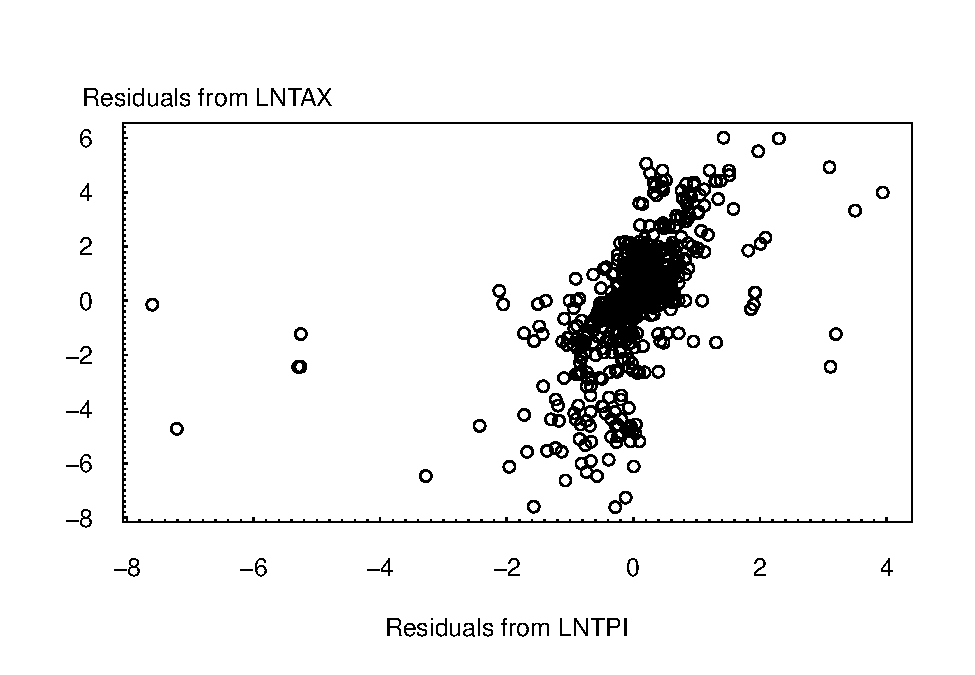
\includegraphics{LongPanelDataScripts_files/figure-latex/unnamed-chunk-33-1.pdf}

\hypertarget{display-3.1---error-components-model}{%
\subsection{DISPLAY 3.1 - Error components model}\label{display-3.1---error-components-model}}

The estimated model appears in Display 3.1, from a fit using the statistical package SAS. Display 3.1 shows that HH, EMP, LNTPI, and MR are statistically significant variables that affect LNTAX. Somewhat surprisingly, the PREP variable was not statistically significant.

\begin{Shaded}
\begin{Highlighting}[]
\NormalTok{random<-}\KeywordTok{lme}\NormalTok{(LNTAX}\OperatorTok{~}\NormalTok{MS}\OperatorTok{+}\NormalTok{HH}\OperatorTok{+}\NormalTok{AGE}\OperatorTok{+}\NormalTok{EMP}\OperatorTok{+}\NormalTok{PREP}\OperatorTok{+}\NormalTok{LNTPI}\OperatorTok{+}\NormalTok{DEPEND}\OperatorTok{+}\NormalTok{MR, }\DataTypeTok{data=}\NormalTok{taxprep, }\DataTypeTok{random=}\OperatorTok{~}\DecValTok{1}\OperatorTok{|}\NormalTok{SUBJECT, }\DataTypeTok{method=}\StringTok{"ML"}\NormalTok{)}
\CommentTok{## }\AlertTok{NOTE}\CommentTok{* THE DEFAULT METHOD IN lme IS "REML"}
\KeywordTok{summary}\NormalTok{(random)}
\end{Highlighting}
\end{Shaded}

\begin{verbatim}
Linear mixed-effects model fit by maximum likelihood
 Data: taxprep 
       AIC      BIC    logLik
  4813.255 4870.041 -2395.627

Random effects:
 Formula: ~1 | SUBJECT
        (Intercept) Residual
StdDev:   0.9602161 1.368896

Fixed effects: LNTAX ~ MS + HH + AGE + EMP + PREP + LNTPI + DEPEND + MR 
                 Value Std.Error   DF   t-value p-value
(Intercept) -2.9603371 0.5705536 1024 -5.188534  0.0000
MS           0.0373000 0.1824839 1024  0.204402  0.8381
HH          -0.6889876 0.2320057 1024 -2.969702  0.0031
AGE          0.0207431 0.2000035 1024  0.103713  0.9174
EMP         -0.5048035 0.1679848 1024 -3.005054  0.0027
PREP        -0.0217036 0.1175229 1024 -0.184675  0.8535
LNTPI        0.7604058 0.0699692 1024 10.867728  0.0000
DEPEND      -0.1127475 0.0592818 1024 -1.901891  0.0575
MR           0.1153752 0.0073142 1024 15.774213  0.0000
 Correlation: 
       (Intr) MS     HH     AGE    EMP    PREP   LNTPI  DEPEND
MS      0.176                                                 
HH      0.030  0.419                                          
AGE    -0.043 -0.167 -0.023                                   
EMP    -0.116 -0.069  0.024 -0.030                            
PREP   -0.035 -0.045  0.004 -0.115 -0.112                     
LNTPI  -0.948 -0.180 -0.081 -0.043  0.099 -0.016              
DEPEND -0.074 -0.604 -0.269  0.224 -0.038 -0.039 -0.068       
MR      0.522 -0.020  0.055  0.149 -0.041 -0.051 -0.698  0.102

Standardized Within-Group Residuals:
        Min          Q1         Med          Q3         Max 
-5.83483692 -0.21263981  0.09677632  0.39814646  5.79731648 

Number of Observations: 1290
Number of Groups: 258 
\end{verbatim}

\hypertarget{section-3.3---random-coefficients-model}{%
\section{SECTION 3.3 - Random coefficients model}\label{section-3.3---random-coefficients-model}}

\begin{Shaded}
\begin{Highlighting}[]
\CommentTok{#randomcoeff<-lme(LNTAX~MS+HH+AGE+EMP+PREP+LNTPI+DEPEND+MR, data=taxprep, random=~1+MS+HH+AGE+EMP+PREP+LNTPI+DEPEND+MR|SUBJECT, method="ML") }
\CommentTok{# }\AlertTok{NOTE}\CommentTok{*:It takes forever to run the estimation, in the end a warning messaged was given. }
\CommentTok{# No estimation result was produced. }
\CommentTok{# The reason is due to the fact that in SAS, the method of mivque0 allows estimation for this model, in R this method is not readily available to be coded.}
\end{Highlighting}
\end{Shaded}

\hypertarget{prediction-and-bayesian-inference}{%
\chapter{Prediction and Bayesian Inference}\label{prediction-and-bayesian-inference}}

\hypertarget{import-data-3}{%
\section{Import Data}\label{import-data-3}}

\begin{Shaded}
\begin{Highlighting}[]
\NormalTok{lottery  =}\StringTok{ }\KeywordTok{read.table}\NormalTok{(}\StringTok{"TXTData/Lottery.txt"}\NormalTok{, }\DataTypeTok{sep =}\StringTok{"}\CharTok{\textbackslash{}t}\StringTok{"}\NormalTok{, }\DataTypeTok{quote =} \StringTok{""}\NormalTok{,}\DataTypeTok{header=}\OtherTok{TRUE}\NormalTok{)}

\CommentTok{#lottery=read.table(choose.files(), header=TRUE, sep="\textbackslash{}t")}
\end{Highlighting}
\end{Shaded}

State of Wisconsin lottery administrators provided weekly lottery sales data. We consider online lottery tickets that are sold by selected retail establishments in Wisconsin. These tickets are generally priced at \$1.00, so the number of tickets sold equals the lottery revenue. We analyze lottery sales (\texttt{OLSALES}) over a forty-week period, April, 1998 through January, 1999, from fifty randomly selected ZIP codes within the state of Wisconsin. We also consider the number of retailers within a ZIP code for each time (\texttt{NRETAIL}).

\begin{longtable}[]{@{}ll@{}}
\toprule
Variable & Description\tabularnewline
\midrule
\endhead
OLSALES & Online lottery sales to individual consumers\tabularnewline
NRETAIL & Number of listed retailers\tabularnewline
PERPERHH & Persons per household MEDSCHYR Median years of schooling\tabularnewline
MEDHVL & Median home value in \$1000s for owner-occupied homes PRCRENT\tabularnewline
PRC55P & Percent of population that is 55 or older\tabularnewline
HHMEDAGE & Household median age\tabularnewline
MEDINC & Estimated median household income, in \$1000s\tabularnewline
POPULATN & Population, in thousands\tabularnewline
\bottomrule
\end{longtable}

\begin{Shaded}
\begin{Highlighting}[]
\CommentTok{#EXTRACT TIME - INVARIANT INFORMATION TO ANALYZE}
\NormalTok{mzip=d=}\KeywordTok{as.data.frame}\NormalTok{(}\KeywordTok{t}\NormalTok{(}\KeywordTok{sapply}\NormalTok{(}\KeywordTok{split}\NormalTok{(lottery[, }\KeywordTok{c}\NormalTok{(}\StringTok{"NRETAIL"}\NormalTok{, }\StringTok{"PERPERHH"}\NormalTok{, }\StringTok{"OLSALES"}\NormalTok{, }\StringTok{"MEDSCHYR"}\NormalTok{, }\StringTok{"MEDHVL"}\NormalTok{, }\StringTok{"PRCRENT"}\NormalTok{, }\StringTok{"PRC55P"}\NormalTok{, }\StringTok{"HHMEDAGE"}\NormalTok{, }\StringTok{"MEDINC"}\NormalTok{, }\StringTok{"POPULATN"}\NormalTok{)], lottery}\OperatorTok{$}\NormalTok{ZIP),}\ControlFlowTok{function}\NormalTok{(x) }\KeywordTok{colMeans}\NormalTok{(x))))}
 \CommentTok{# Extract time invariant information to analyze}
\CommentTok{# Notice: the code for this part on website is wrong.}
\end{Highlighting}
\end{Shaded}

\hypertarget{example-forecasting-wisconsin-lottery-sales-page-138}{%
\section{Example: Forecasting Wisconsin Lottery Sales (Page 138)}\label{example-forecasting-wisconsin-lottery-sales-page-138}}

In this section, we forecast the sale of state lottery tickets from 50 postal (ZIP) codes inWisconsin. Lottery sales are an important component of state revenues. Accurate forecasting helps in the budget-planning process. A model is useful in assessing the important determinants of lottery sales, and understanding the determinants of lottery sales is useful for improving the design of the lottery sales system. Additional details of this study are in Frees and Miller (2003O).

\hypertarget{table-4.2-time---invariant-summary-statistics}{%
\subsection{TABLE 4.2: Time - invariant summary statistics}\label{table-4.2-time---invariant-summary-statistics}}

\begin{Shaded}
\begin{Highlighting}[]
\KeywordTok{summary}\NormalTok{(mzip[,}\KeywordTok{c}\NormalTok{(}\StringTok{"NRETAIL"}\NormalTok{, }\StringTok{"PERPERHH"}\NormalTok{, }\StringTok{"OLSALES"}\NormalTok{, }\StringTok{"MEDSCHYR"}\NormalTok{, }\StringTok{"MEDHVL"}\NormalTok{, }\StringTok{"PRCRENT"}\NormalTok{, }\StringTok{"PRC55P"}\NormalTok{, }\StringTok{"HHMEDAGE"}\NormalTok{, }\StringTok{"MEDINC"}\NormalTok{, }\StringTok{"POPULATN"}\NormalTok{)]) }
\end{Highlighting}
\end{Shaded}

\begin{verbatim}
    NRETAIL          PERPERHH        OLSALES           MEDSCHYR    
 Min.   : 1.000   Min.   :2.200   Min.   :  189.0   Min.   :12.20  
 1st Qu.: 3.000   1st Qu.:2.600   1st Qu.:  821.3   1st Qu.:12.50  
 Median : 6.362   Median :2.700   Median : 2426.4   Median :12.60  
 Mean   :11.942   Mean   :2.706   Mean   : 6494.8   Mean   :12.70  
 3rd Qu.:15.312   3rd Qu.:2.800   3rd Qu.:10016.5   3rd Qu.:12.78  
 Max.   :68.625   Max.   :3.200   Max.   :33181.4   Max.   :15.90  
     MEDHVL          PRCRENT          PRC55P        HHMEDAGE    
 Min.   : 34.50   Min.   : 6.00   Min.   :25.0   Min.   :41.00  
 1st Qu.: 43.77   1st Qu.:19.25   1st Qu.:35.0   1st Qu.:46.00  
 Median : 53.90   Median :24.00   Median :40.0   Median :48.00  
 Mean   : 57.09   Mean   :24.68   Mean   :39.7   Mean   :48.76  
 3rd Qu.: 66.47   3rd Qu.:27.00   3rd Qu.:44.0   3rd Qu.:51.00  
 Max.   :120.00   Max.   :62.00   Max.   :56.0   Max.   :59.00  
     MEDINC         POPULATN     
 Min.   :27.90   Min.   : 0.280  
 1st Qu.:38.17   1st Qu.: 1.964  
 Median :43.10   Median : 4.405  
 Mean   :45.12   Mean   : 9.311  
 3rd Qu.:53.62   3rd Qu.:15.446  
 Max.   :70.70   Max.   :39.098  
\end{verbatim}

\begin{Shaded}
\begin{Highlighting}[]
\CommentTok{# STANDARD DEVIATION}
\KeywordTok{sqrt}\NormalTok{(}\KeywordTok{diag}\NormalTok{(}\KeywordTok{var}\NormalTok{(mzip[,}\KeywordTok{c}\NormalTok{(}\StringTok{"NRETAIL"}\NormalTok{, }\StringTok{"PERPERHH"}\NormalTok{, }\StringTok{"OLSALES"}\NormalTok{, }\StringTok{"MEDSCHYR"}\NormalTok{, }\StringTok{"MEDHVL"}\NormalTok{, }\StringTok{"PRCRENT"}\NormalTok{, }\StringTok{"PRC55P"}\NormalTok{, }\StringTok{"HHMEDAGE"}\NormalTok{, }\StringTok{"MEDINC"}\NormalTok{, }\StringTok{"POPULATN"}\NormalTok{)]))) }
\end{Highlighting}
\end{Shaded}

\begin{verbatim}
     NRETAIL     PERPERHH      OLSALES     MEDSCHYR       MEDHVL 
  13.2918231    0.2093820 8103.0125037    0.5514212   18.3731152 
     PRCRENT       PRC55P     HHMEDAGE       MEDINC     POPULATN 
   9.3425513    7.5112161    4.1431527    9.7835616   11.0981570 
\end{verbatim}

\hypertarget{figure-4.2-look-at-the-relationship}{%
\subsection{FIGURE 4.2: Look at the relationship}\label{figure-4.2-look-at-the-relationship}}

Figure 4.2 shows a positive relationship between average online sales and population. Further, the ZIP code corresponding to the city of Kenosha, Wisconsin, has unusually large average sales for its population size.

\begin{Shaded}
\begin{Highlighting}[]
\KeywordTok{plot}\NormalTok{(OLSALES }\OperatorTok{~}\StringTok{ }\NormalTok{POPULATN, }\DataTypeTok{data =}\NormalTok{ mzip, }\DataTypeTok{xlab=}\StringTok{""}\NormalTok{, }\DataTypeTok{ylab=}\StringTok{""}\NormalTok{, }\DataTypeTok{xaxt=}\StringTok{"n"}\NormalTok{, }\DataTypeTok{yaxt=}\StringTok{"n"}\NormalTok{,}\DataTypeTok{pch=}\StringTok{"o"}\NormalTok{, }\DataTypeTok{las=}\DecValTok{1}\NormalTok{, }\DataTypeTok{cex=}\DecValTok{1}\NormalTok{)}

\KeywordTok{axis}\NormalTok{(}\DecValTok{2}\NormalTok{, }\DataTypeTok{at=}\KeywordTok{seq}\NormalTok{(}\DecValTok{0}\NormalTok{, }\DecValTok{40000}\NormalTok{, }\DataTypeTok{by=}\DecValTok{10000}\NormalTok{), }\DataTypeTok{las=}\DecValTok{1}\NormalTok{, }\DataTypeTok{font=}\DecValTok{10}\NormalTok{, }\DataTypeTok{cex=}\FloatTok{0.005}\NormalTok{, }\DataTypeTok{tck=}\FloatTok{0.01}\NormalTok{)}

\KeywordTok{axis}\NormalTok{(}\DecValTok{2}\NormalTok{, }\DataTypeTok{at=}\KeywordTok{seq}\NormalTok{(}\DecValTok{0}\NormalTok{, }\DecValTok{40000}\NormalTok{, }\DataTypeTok{by=}\DecValTok{1000}\NormalTok{), }\DataTypeTok{lab=}\NormalTok{F, }\DataTypeTok{tck=}\FloatTok{0.005}\NormalTok{)}

\KeywordTok{axis}\NormalTok{(}\DecValTok{1}\NormalTok{, }\DataTypeTok{at=}\KeywordTok{seq}\NormalTok{(}\DecValTok{0}\NormalTok{,}\DecValTok{40}\NormalTok{, }\DataTypeTok{by=}\DecValTok{10}\NormalTok{), }\DataTypeTok{font=}\DecValTok{10}\NormalTok{, }\DataTypeTok{cex=}\FloatTok{0.005}\NormalTok{, }\DataTypeTok{tck=}\FloatTok{0.01}\NormalTok{)}

\KeywordTok{axis}\NormalTok{(}\DecValTok{1}\NormalTok{, }\DataTypeTok{at=}\KeywordTok{seq}\NormalTok{(}\DecValTok{0}\NormalTok{,}\DecValTok{40}\NormalTok{, }\DataTypeTok{by=}\DecValTok{1}\NormalTok{), }\DataTypeTok{lab=}\NormalTok{F, }\DataTypeTok{tck=}\FloatTok{0.005}\NormalTok{)}

\KeywordTok{mtext}\NormalTok{(}\StringTok{"Average Lottery Sales"}\NormalTok{, }\DataTypeTok{side=}\DecValTok{2}\NormalTok{, }\DataTypeTok{line=}\OperatorTok{-}\FloatTok{3.5}\NormalTok{, }\DataTypeTok{at=}\DecValTok{36000}\NormalTok{, }\DataTypeTok{font=}\DecValTok{10}\NormalTok{, }\DataTypeTok{cex=}\DecValTok{1}\NormalTok{, }\DataTypeTok{las=}\DecValTok{1}\NormalTok{)}

\KeywordTok{mtext}\NormalTok{(}\StringTok{"Population in Thousands"}\NormalTok{, }\DataTypeTok{side=}\DecValTok{1}\NormalTok{, }\DataTypeTok{line=}\DecValTok{2}\NormalTok{, }\DataTypeTok{at=}\DecValTok{20}\NormalTok{, }\DataTypeTok{font=}\DecValTok{10}\NormalTok{, }\DataTypeTok{cex=}\DecValTok{1}\NormalTok{, }\DataTypeTok{las=}\DecValTok{1}\NormalTok{)}
\end{Highlighting}
\end{Shaded}

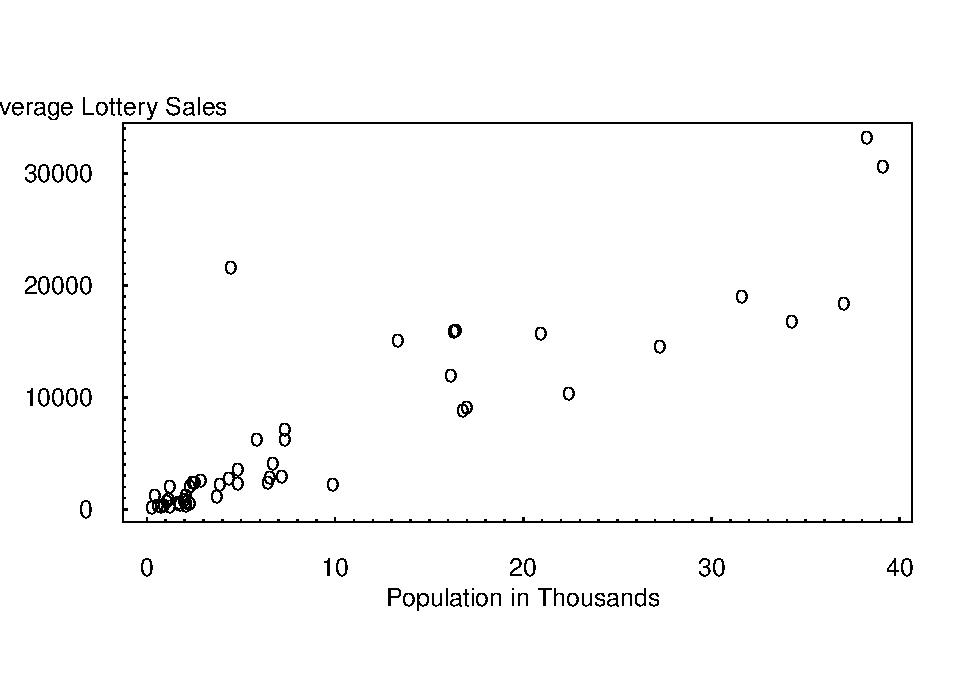
\includegraphics{LongPanelDataScripts_files/figure-latex/unnamed-chunk-40-1.pdf}

\hypertarget{sorting-the-data-by-zip-then-combine-vectors-into-another-data.frame}{%
\subsection{Sorting the data by zip then combine vectors into another data.frame}\label{sorting-the-data-by-zip-then-combine-vectors-into-another-data.frame}}

\begin{Shaded}
\begin{Highlighting}[]
\NormalTok{lottery}\OperatorTok{$}\NormalTok{logsales<-}\KeywordTok{log10}\NormalTok{(lottery}\OperatorTok{$}\NormalTok{OLSALES)}
\NormalTok{m<-}\KeywordTok{order}\NormalTok{(lottery}\OperatorTok{$}\NormalTok{ZIP, lottery}\OperatorTok{$}\NormalTok{TIME, lottery}\OperatorTok{$}\NormalTok{OLSALES,lottery}\OperatorTok{$}\NormalTok{logsales)}

\NormalTok{index<-}\KeywordTok{as.data.frame}\NormalTok{(}\KeywordTok{cbind}\NormalTok{(lottery}\OperatorTok{$}\NormalTok{ZIP[m],lottery}\OperatorTok{$}\NormalTok{TIME[m],lottery}\OperatorTok{$}\NormalTok{OLSALES[m],lottery}\OperatorTok{$}\NormalTok{logsales[m]))}

\KeywordTok{names}\NormalTok{(index)<-}\KeywordTok{c}\NormalTok{(}\StringTok{"ZIP"}\NormalTok{, }\StringTok{"TIME"}\NormalTok{, }\StringTok{"OLSALES"}\NormalTok{, }\StringTok{"LOGSALES"}\NormalTok{)}
\end{Highlighting}
\end{Shaded}

\hypertarget{figure-4.3-lottery-vs.-week-number}{%
\subsection{FIGURE 4.3: Lottery vs.~week number}\label{figure-4.3-lottery-vs.-week-number}}

Figure 4.3 presents a multiple time-series plot of (weekly) sales over time. Here, each line traces the sales patterns for a particular ZIP code. This figure shows the dramatic increase in sales for most ZIP codes, at approximately weeks 8 and 18.

\begin{Shaded}
\begin{Highlighting}[]
\KeywordTok{plot}\NormalTok{(OLSALES }\OperatorTok{~}\StringTok{ }\NormalTok{TIME, }\DataTypeTok{data =}\NormalTok{ lottery, }\DataTypeTok{axes=}\NormalTok{F, }\DataTypeTok{ylab=}\StringTok{""}\NormalTok{, }\DataTypeTok{xlab=}\StringTok{""}\NormalTok{, }\DataTypeTok{xaxt=}\StringTok{"n"}\NormalTok{, }\DataTypeTok{yaxt=}\StringTok{"n"}\NormalTok{)}
\ControlFlowTok{for}\NormalTok{ (i }\ControlFlowTok{in}\NormalTok{ index}\OperatorTok{$}\NormalTok{ZIP) \{}
     \KeywordTok{lines}\NormalTok{(OLSALES }\OperatorTok{~}\StringTok{ }\NormalTok{TIME, }\DataTypeTok{data =} \KeywordTok{subset}\NormalTok{(index, ZIP }\OperatorTok{==}\StringTok{ }\NormalTok{i)) \}}
\KeywordTok{axis}\NormalTok{(}\DecValTok{1}\NormalTok{, }\DataTypeTok{at=}\KeywordTok{seq}\NormalTok{(}\DecValTok{0}\NormalTok{,}\DecValTok{40}\NormalTok{, }\DataTypeTok{by=}\DecValTok{1}\NormalTok{), }\DataTypeTok{labels=}\NormalTok{F, }\DataTypeTok{tck=}\FloatTok{0.005}\NormalTok{)}
\KeywordTok{axis}\NormalTok{(}\DecValTok{1}\NormalTok{, }\DataTypeTok{at=}\KeywordTok{seq}\NormalTok{(}\DecValTok{0}\NormalTok{,}\DecValTok{40}\NormalTok{, }\DataTypeTok{by=}\DecValTok{10}\NormalTok{), }\DataTypeTok{cex=}\FloatTok{0.005}\NormalTok{, }\DataTypeTok{tck=}\FloatTok{0.01}\NormalTok{)}
\KeywordTok{mtext}\NormalTok{(}\StringTok{"Week Number"}\NormalTok{, }\DataTypeTok{side=}\DecValTok{1}\NormalTok{, }\DataTypeTok{line=}\FloatTok{2.5}\NormalTok{, }\DataTypeTok{cex=}\DecValTok{1}\NormalTok{, }\DataTypeTok{font=}\DecValTok{10}\NormalTok{)}
\KeywordTok{axis}\NormalTok{(}\DecValTok{2}\NormalTok{, }\DataTypeTok{at=}\KeywordTok{seq}\NormalTok{(}\DecValTok{0}\NormalTok{, }\DecValTok{300000}\NormalTok{, }\DataTypeTok{by=}\DecValTok{10000}\NormalTok{), }\DataTypeTok{labels=}\NormalTok{F, }\DataTypeTok{tck=}\FloatTok{0.005}\NormalTok{)}
\KeywordTok{axis}\NormalTok{(}\DecValTok{2}\NormalTok{, }\DataTypeTok{at=}\KeywordTok{seq}\NormalTok{(}\DecValTok{0}\NormalTok{, }\DecValTok{305000}\NormalTok{, }\DataTypeTok{by=}\DecValTok{100000}\NormalTok{), }\DataTypeTok{las=}\DecValTok{1}\NormalTok{, }\DataTypeTok{cex=}\FloatTok{0.005}\NormalTok{, }\DataTypeTok{tck=}\FloatTok{0.01}\NormalTok{) }
\KeywordTok{mtext}\NormalTok{(}\StringTok{"Lottery Sales"}\NormalTok{, }\DataTypeTok{side=}\DecValTok{2}\NormalTok{, }\DataTypeTok{line=}\OperatorTok{-}\DecValTok{3}\NormalTok{, }\DataTypeTok{at=}\DecValTok{310000}\NormalTok{, }\DataTypeTok{font=}\DecValTok{10}\NormalTok{, }\DataTypeTok{cex=}\DecValTok{1}\NormalTok{, }\DataTypeTok{las=}\DecValTok{1}\NormalTok{)}
\end{Highlighting}
\end{Shaded}

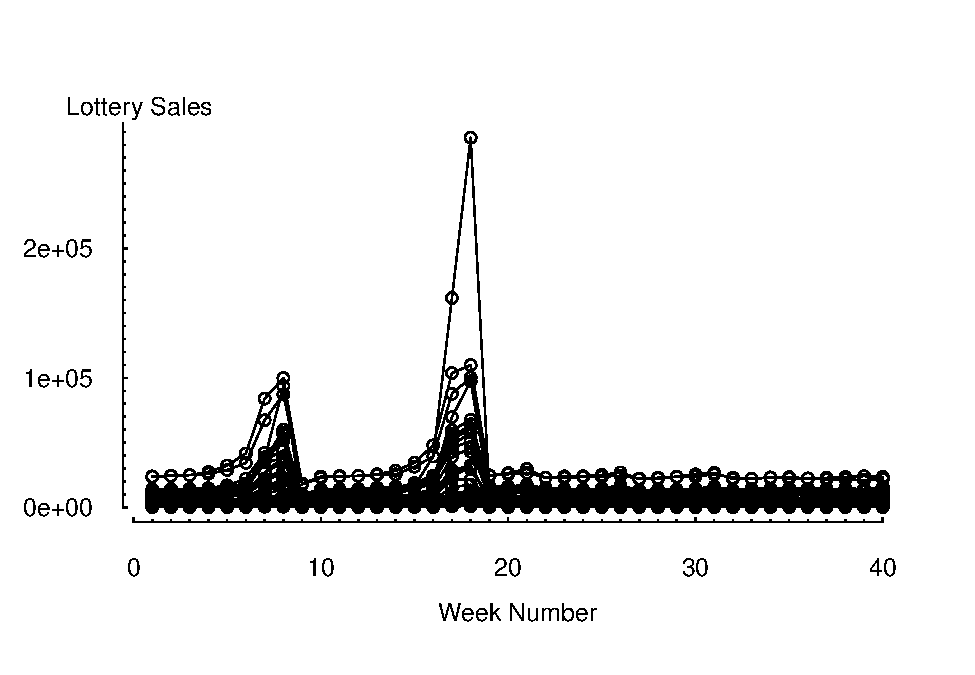
\includegraphics{LongPanelDataScripts_files/figure-latex/unnamed-chunk-42-1.pdf}

Another way of producing multiple time series graph by using trellis xyplot:

\begin{Shaded}
\begin{Highlighting}[]
\KeywordTok{library}\NormalTok{(lattice)}
\KeywordTok{trellis.device}\NormalTok{(}\DataTypeTok{color=}\NormalTok{F) }\CommentTok{# telling the trellis device to mimic 'black and white'}
\KeywordTok{xyplot}\NormalTok{(OLSALES }\OperatorTok{~}\StringTok{ }\NormalTok{TIME, }\DataTypeTok{data=}\NormalTok{index, }\DataTypeTok{groups=}\NormalTok{ZIP, }\DataTypeTok{scales=}\KeywordTok{list}\NormalTok{(}\DataTypeTok{y=}\KeywordTok{list}\NormalTok{(}\DataTypeTok{at=}\KeywordTok{seq}\NormalTok{(}\DecValTok{0}\NormalTok{, }\DecValTok{300000}\NormalTok{,}\DecValTok{100000}\NormalTok{), }\DataTypeTok{tck=}\NormalTok{.}\DecValTok{01}\NormalTok{)), }\DataTypeTok{panel=}\NormalTok{panel.superpose, }\DataTypeTok{pch=}\DecValTok{16}\NormalTok{, }\DataTypeTok{lty=}\DecValTok{1}\NormalTok{,  }\DataTypeTok{type=}\StringTok{"b"}\NormalTok{)}

\CommentTok{#ChECK LOG VALUES}
\NormalTok{lottery}\OperatorTok{$}\NormalTok{logsales<-}\KeywordTok{log10}\NormalTok{(lottery}\OperatorTok{$}\NormalTok{OLSALES)}
\NormalTok{lottery}\OperatorTok{$}\NormalTok{lnsales<-}\KeywordTok{log}\NormalTok{(lottery}\OperatorTok{$}\NormalTok{OLSALES)}
\end{Highlighting}
\end{Shaded}

\hypertarget{figure-4.4-log-lottery-vs-week-number}{%
\subsection{FIGURE 4.4: Log lottery vs week number}\label{figure-4.4-log-lottery-vs-week-number}}

Figure 4.4 shows the same information as in Figure 4.3 but on a common (base 10) logarithmic scale. Here, we still see the effects of the PowerBall jackpots on sales. However, Figure 4.4 suggests a dynamic pattern that is common to all ZIP codes. Specifically, logarithmic sales for each ZIP code are relatively stable with the same approximate level of variability. Further, logarithmic sales for each ZIP code peak at the same time, corresponding to large PowerBall jackpots.

\begin{Shaded}
\begin{Highlighting}[]
\CommentTok{#FIGURE 4.4 LOG LOTTERY vs WEEK NUMBER}
\KeywordTok{plot}\NormalTok{(LOGSALES }\OperatorTok{~}\StringTok{ }\NormalTok{TIME, }\DataTypeTok{data =}\NormalTok{ index, }\DataTypeTok{type=}\StringTok{"p"}\NormalTok{, }\DataTypeTok{axes=}\NormalTok{F, }\DataTypeTok{ylab=}\StringTok{""}\NormalTok{, }\DataTypeTok{xlab=}\StringTok{""}\NormalTok{, }\DataTypeTok{pch=}\DecValTok{16}\NormalTok{, }\DataTypeTok{mkh=}\FloatTok{0.0001}\NormalTok{, }\DataTypeTok{lwd=}\FloatTok{0.5}\NormalTok{)}
\KeywordTok{axis}\NormalTok{(}\DecValTok{1}\NormalTok{, }\DataTypeTok{at=}\KeywordTok{seq}\NormalTok{(}\DecValTok{0}\NormalTok{,}\DecValTok{40}\NormalTok{, }\DataTypeTok{by=}\DecValTok{1}\NormalTok{), }\DataTypeTok{labels=}\NormalTok{F, }\DataTypeTok{tck=}\FloatTok{0.005}\NormalTok{)}
\KeywordTok{axis}\NormalTok{(}\DecValTok{1}\NormalTok{, }\DataTypeTok{at=}\KeywordTok{seq}\NormalTok{(}\DecValTok{0}\NormalTok{,}\DecValTok{40}\NormalTok{, }\DataTypeTok{by=}\DecValTok{10}\NormalTok{), }\DataTypeTok{cex=}\FloatTok{0.4}\NormalTok{, }\DataTypeTok{tck=}\FloatTok{0.01}\NormalTok{)}
\KeywordTok{mtext}\NormalTok{(}\StringTok{"Week Number"}\NormalTok{, }\DataTypeTok{side=}\DecValTok{1}\NormalTok{, }\DataTypeTok{line=}\FloatTok{2.5}\NormalTok{, }\DataTypeTok{cex=}\FloatTok{0.7}\NormalTok{, }\DataTypeTok{font=}\DecValTok{10}\NormalTok{)}
\KeywordTok{axis}\NormalTok{(}\DecValTok{2}\NormalTok{, }\DataTypeTok{at=}\KeywordTok{seq}\NormalTok{(}\DecValTok{0}\NormalTok{, }\DecValTok{6}\NormalTok{, }\DataTypeTok{by=}\FloatTok{0.1}\NormalTok{), }\DataTypeTok{labels=}\NormalTok{F, }\DataTypeTok{tck=}\FloatTok{0.005}\NormalTok{)}
\KeywordTok{axis}\NormalTok{(}\DecValTok{2}\NormalTok{, }\DataTypeTok{at=}\KeywordTok{seq}\NormalTok{(}\DecValTok{0}\NormalTok{, }\DecValTok{6}\NormalTok{, }\DataTypeTok{by=}\DecValTok{1}\NormalTok{), }\DataTypeTok{las=}\DecValTok{1}\NormalTok{, }\DataTypeTok{cex=}\FloatTok{0.4}\NormalTok{, }\DataTypeTok{tck=}\FloatTok{0.01}\NormalTok{) }
\KeywordTok{mtext}\NormalTok{(}\StringTok{"Logarithmic Lottery Sales"}\NormalTok{, }\DataTypeTok{side=}\DecValTok{2}\NormalTok{, }\DataTypeTok{line=}\OperatorTok{-}\DecValTok{1}\NormalTok{, }\DataTypeTok{at=}\FloatTok{5.8}\NormalTok{, }\DataTypeTok{font=}\DecValTok{10}\NormalTok{, }\DataTypeTok{cex=}\FloatTok{0.7}\NormalTok{, }\DataTypeTok{las=}\DecValTok{1}\NormalTok{)}
    \ControlFlowTok{for}\NormalTok{ (i }\ControlFlowTok{in}\NormalTok{ index}\OperatorTok{$}\NormalTok{ZIP) \{}
    \KeywordTok{lines}\NormalTok{(LOGSALES }\OperatorTok{~}\StringTok{ }\NormalTok{TIME, }\DataTypeTok{data=}\KeywordTok{subset}\NormalTok{(index, ZIP}\OperatorTok{==}\NormalTok{i)) \}}
\end{Highlighting}
\end{Shaded}

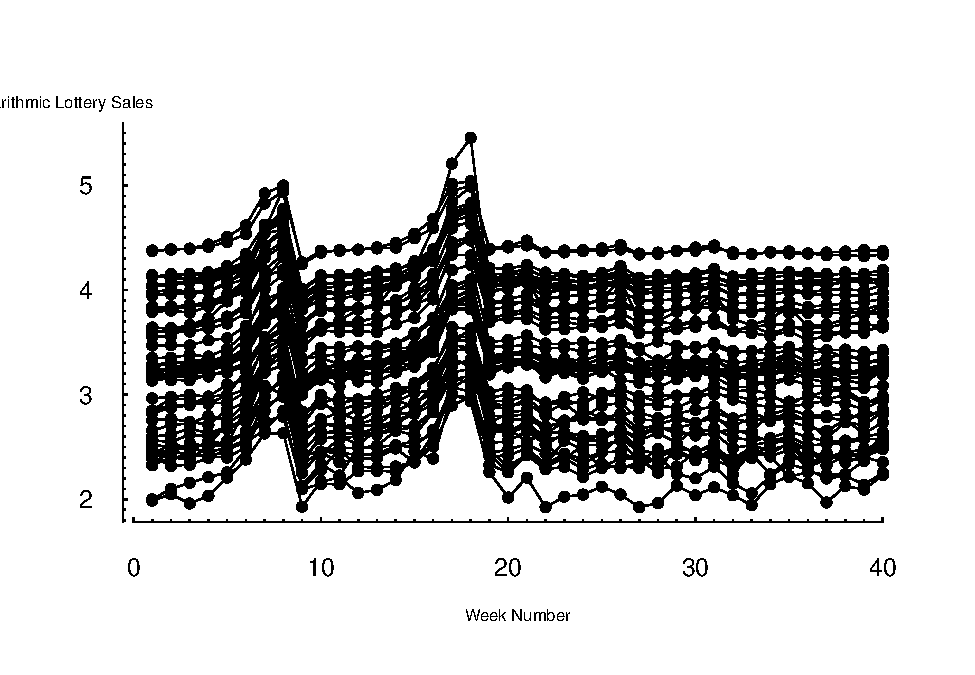
\includegraphics{LongPanelDataScripts_files/figure-latex/unnamed-chunk-44-1.pdf}

\hypertarget{create-model-development-sample}{%
\section{Create model development sample}\label{create-model-development-sample}}

\begin{Shaded}
\begin{Highlighting}[]
\NormalTok{Lottery=lottery}
\NormalTok{Lottery}\OperatorTok{$}\NormalTok{LNSALES<-}\KeywordTok{log}\NormalTok{(Lottery}\OperatorTok{$}\NormalTok{OLSALES)}
\NormalTok{Lottery2<-}\KeywordTok{subset}\NormalTok{(Lottery, Lottery}\OperatorTok{$}\NormalTok{TIME}\OperatorTok{<}\DecValTok{36}\NormalTok{)}
\end{Highlighting}
\end{Shaded}

\hypertarget{model-1.-pooled-cross-setional-model}{%
\subsection{MODEL 1. Pooled cross-setional model}\label{model-1.-pooled-cross-setional-model}}

\begin{Shaded}
\begin{Highlighting}[]
\NormalTok{lm1<-}\KeywordTok{lm}\NormalTok{(LNSALES}\OperatorTok{~}\NormalTok{PERPERHH}\OperatorTok{+}\NormalTok{MEDSCHYR}\OperatorTok{+}\NormalTok{MEDHVL}\OperatorTok{+}\NormalTok{PRCRENT}\OperatorTok{+}\NormalTok{PRC55P}\OperatorTok{+}\NormalTok{HHMEDAGE}\OperatorTok{+}\NormalTok{MEDINC}\OperatorTok{+}\NormalTok{POPULATN}\OperatorTok{+}\NormalTok{NRETAIL, }\DataTypeTok{data=}\NormalTok{Lottery2)}
\KeywordTok{summary}\NormalTok{(lm1)}
\end{Highlighting}
\end{Shaded}

\begin{verbatim}

Call:
lm(formula = LNSALES ~ PERPERHH + MEDSCHYR + MEDHVL + PRCRENT + 
    PRC55P + HHMEDAGE + MEDINC + POPULATN + NRETAIL, data = Lottery2)

Residuals:
    Min      1Q  Median      3Q     Max 
-1.9743 -0.6012 -0.0774  0.5430  4.2015 

Coefficients:
             Estimate Std. Error t value Pr(>|t|)    
(Intercept) 13.821060   1.339594  10.317  < 2e-16 ***
PERPERHH    -1.084705   0.160224  -6.770 1.76e-11 ***
MEDSCHYR    -0.821644   0.069049 -11.899  < 2e-16 ***
MEDHVL       0.013822   0.002662   5.192 2.33e-07 ***
PRCRENT      0.031820   0.003738   8.512  < 2e-16 ***
PRC55P      -0.069578   0.013397  -5.194 2.30e-07 ***
HHMEDAGE     0.118136   0.020961   5.636 2.03e-08 ***
MEDINC       0.043373   0.005304   8.177 5.53e-16 ***
POPULATN     0.057025   0.006060   9.410  < 2e-16 ***
NRETAIL      0.021278   0.004076   5.220 2.00e-07 ***
---
Signif. codes:  0 '***' 0.001 '**' 0.01 '*' 0.05 '.' 0.1 ' ' 1

Residual standard error: 0.8365 on 1740 degrees of freedom
Multiple R-squared:  0.6963,    Adjusted R-squared:  0.6947 
F-statistic: 443.3 on 9 and 1740 DF,  p-value: < 2.2e-16
\end{verbatim}

\hypertarget{model-2.-error-components-model}{%
\subsection{MODEL 2. Error components model}\label{model-2.-error-components-model}}

\begin{Shaded}
\begin{Highlighting}[]
\KeywordTok{library}\NormalTok{(nlme)}
\NormalTok{lme1<-}\KeywordTok{lme}\NormalTok{(LNSALES}\OperatorTok{~}\NormalTok{PERPERHH}\OperatorTok{+}\NormalTok{MEDSCHYR}\OperatorTok{+}\NormalTok{MEDHVL}\OperatorTok{+}\NormalTok{PRCRENT}\OperatorTok{+}\NormalTok{PRC55P}\OperatorTok{+}\NormalTok{HHMEDAGE}\OperatorTok{+}\NormalTok{MEDINC}\OperatorTok{+}\NormalTok{POPULATN}\OperatorTok{+}\NormalTok{NRETAIL, }\DataTypeTok{data=}\NormalTok{Lottery2, }\DataTypeTok{random=}\OperatorTok{~}\DecValTok{1}\OperatorTok{|}\NormalTok{ZIP, }\DataTypeTok{method=}\StringTok{"REML"}\NormalTok{) }
\CommentTok{# }\AlertTok{NOTE}\CommentTok{* THE DEFAULT METHOD IN lme IS "REML"}
\CommentTok{# Use REML method in estimating fixed effects beta coefficients }
\KeywordTok{summary}\NormalTok{(lme1)}
\end{Highlighting}
\end{Shaded}

\begin{verbatim}
Linear mixed-effects model fit by REML
 Data: Lottery2 
       AIC      BIC    logLik
  2907.889 2973.428 -1441.944

Random effects:
 Formula: ~1 | ZIP
        (Intercept)  Residual
StdDev:     0.77897 0.5130729

Fixed effects: LNSALES ~ PERPERHH + MEDSCHYR + MEDHVL + PRCRENT + PRC55P + HHMEDAGE +      MEDINC + POPULATN + NRETAIL 
                Value Std.Error   DF   t-value p-value
(Intercept) 18.095695  7.316764 1699  2.473183  0.0135
PERPERHH    -1.287021  0.886172   41 -1.452337  0.1540
MEDSCHYR    -1.077937  0.375131   41 -2.873491  0.0064
MEDHVL       0.007360  0.014633   41  0.502935  0.6177
PRCRENT      0.026321  0.020660   41  1.274032  0.2098
PRC55P      -0.072547  0.074259   41 -0.976939  0.3343
HHMEDAGE     0.118637  0.116199   41  1.020986  0.3132
MEDINC       0.045540  0.029396   41  1.549194  0.1290
POPULATN     0.121851  0.027529   41  4.426231  0.0001
NRETAIL     -0.027177  0.017420 1699 -1.560055  0.1189
 Correlation: 
         (Intr) PERPER MEDSCH MEDHVL PRCREN PRC55P HHMEDA MEDINC POPULA
PERPERHH -0.632                                                        
MEDSCHYR -0.745  0.204                                                 
MEDHVL    0.303  0.093 -0.394                                          
PRCRENT  -0.198  0.402 -0.258  0.008                                   
PRC55P    0.146  0.236 -0.018  0.069  0.039                            
HHMEDAGE -0.461  0.049  0.109 -0.128  0.151 -0.898                     
MEDINC   -0.171 -0.013  0.080 -0.653  0.214  0.392 -0.200              
POPULATN  0.180 -0.021 -0.228 -0.171 -0.287 -0.035  0.035 -0.050       
NRETAIL  -0.210  0.082  0.246  0.159  0.096  0.014 -0.002 -0.027 -0.847

Standardized Within-Group Residuals:
        Min          Q1         Med          Q3         Max 
-2.06921597 -0.49881173 -0.29717361  0.02767368  6.60150830 

Number of Observations: 1750
Number of Groups: 50 
\end{verbatim}

\begin{Shaded}
\begin{Highlighting}[]
\CommentTok{# CHECK AUTOCORRELATION PATTERNS}
\KeywordTok{ACF}\NormalTok{(lme1, }\DataTypeTok{maxlag=}\DecValTok{10}\NormalTok{) }\CommentTok{#Obtain ACF of residuals from lme1}
\end{Highlighting}
\end{Shaded}

\begin{verbatim}
   lag         ACF
1    0  1.00000000
2    1  0.52724776
3    2  0.10000857
4    3 -0.03788895
5    4 -0.15969734
6    5 -0.23410399
7    6 -0.24984691
8    7 -0.18355756
9    8 -0.02825433
10   9  0.19456638
11  10  0.47143962
12  11  0.17601528
13  12 -0.10862546
14  13 -0.16449717
15  14 -0.31225995
16  15 -0.40819498
\end{verbatim}

\begin{Shaded}
\begin{Highlighting}[]
\KeywordTok{lag.plot}\NormalTok{(lme1}\OperatorTok{$}\NormalTok{residuals, }\DataTypeTok{lags=}\OperatorTok{-}\DecValTok{1}\NormalTok{) }\CommentTok{#Autocorrelation patterns one lag, needs to refine}
\end{Highlighting}
\end{Shaded}

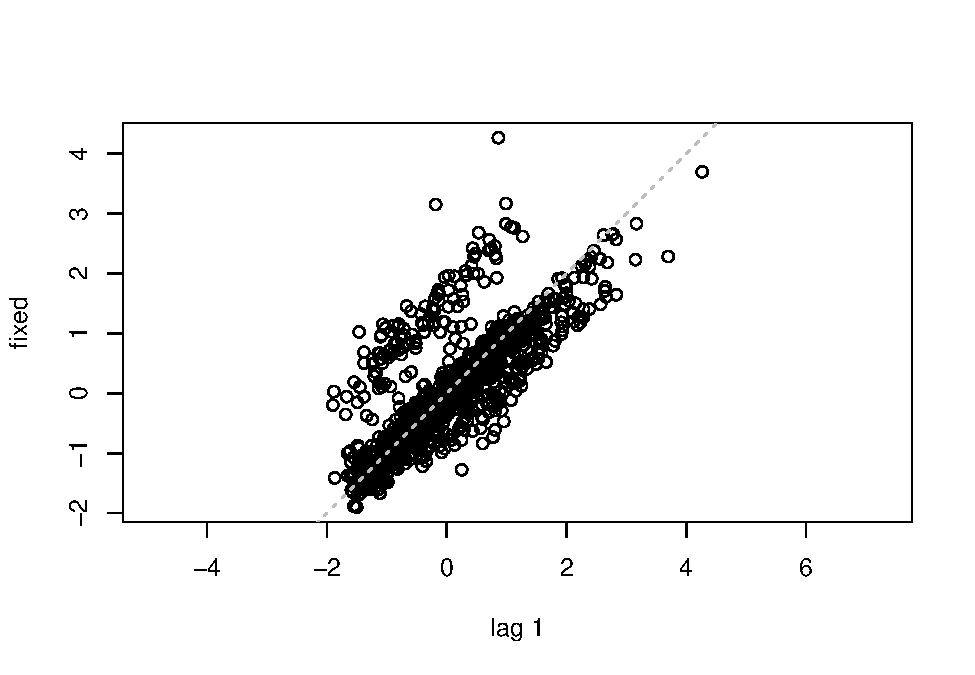
\includegraphics{LongPanelDataScripts_files/figure-latex/unnamed-chunk-48-1.pdf} 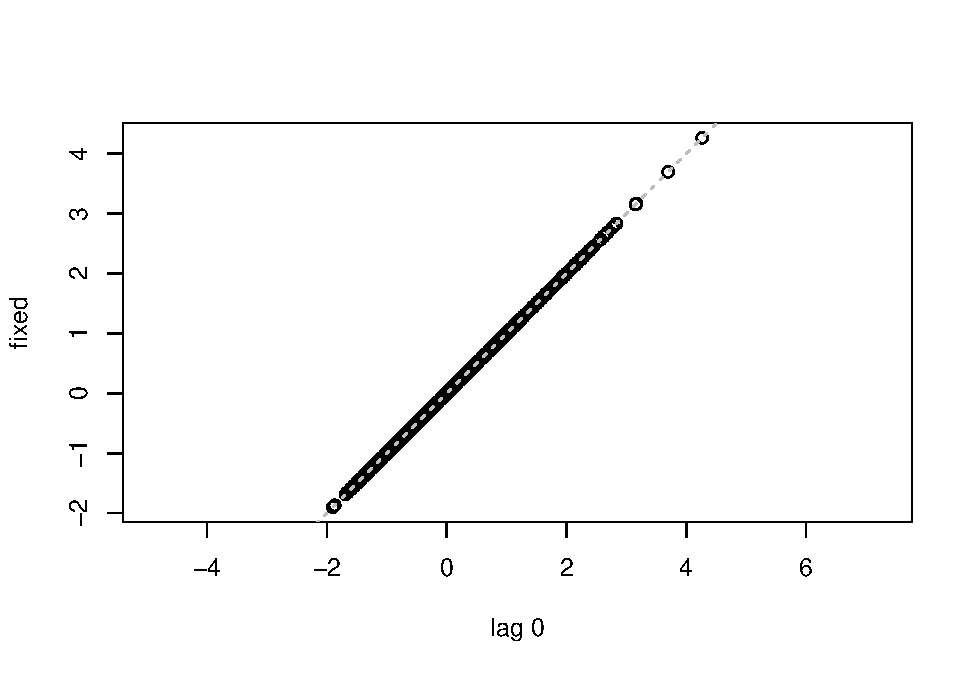
\includegraphics{LongPanelDataScripts_files/figure-latex/unnamed-chunk-48-2.pdf} 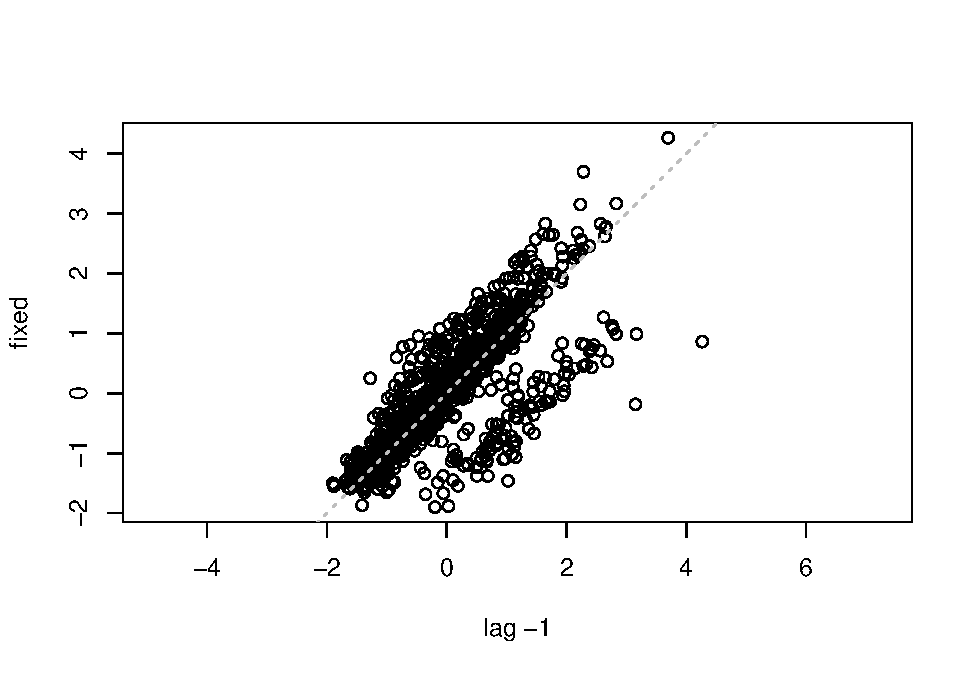
\includegraphics{LongPanelDataScripts_files/figure-latex/unnamed-chunk-48-3.pdf} 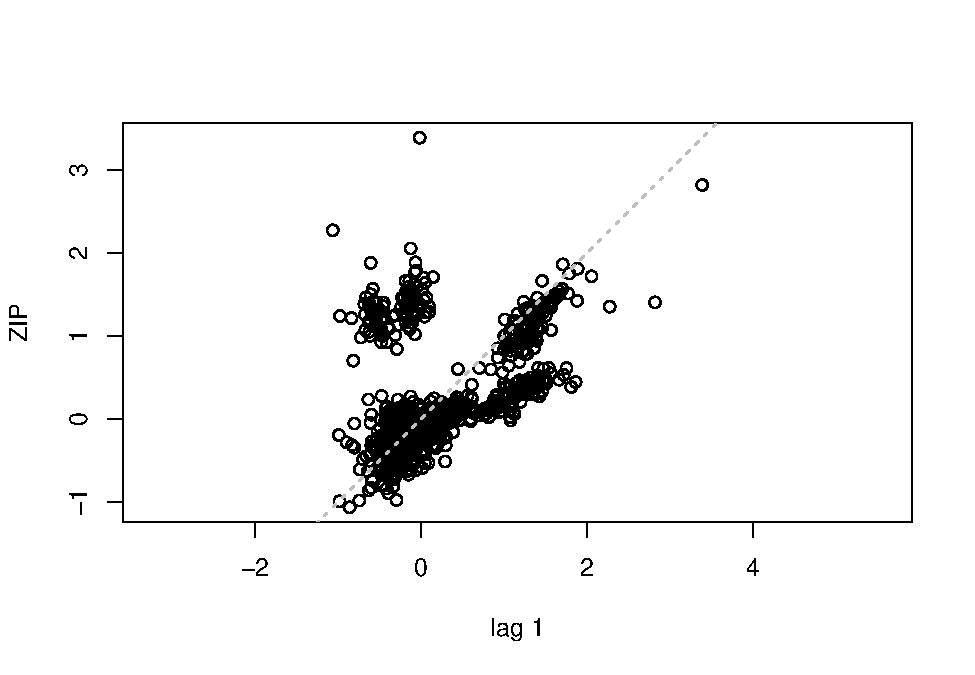
\includegraphics{LongPanelDataScripts_files/figure-latex/unnamed-chunk-48-4.pdf} 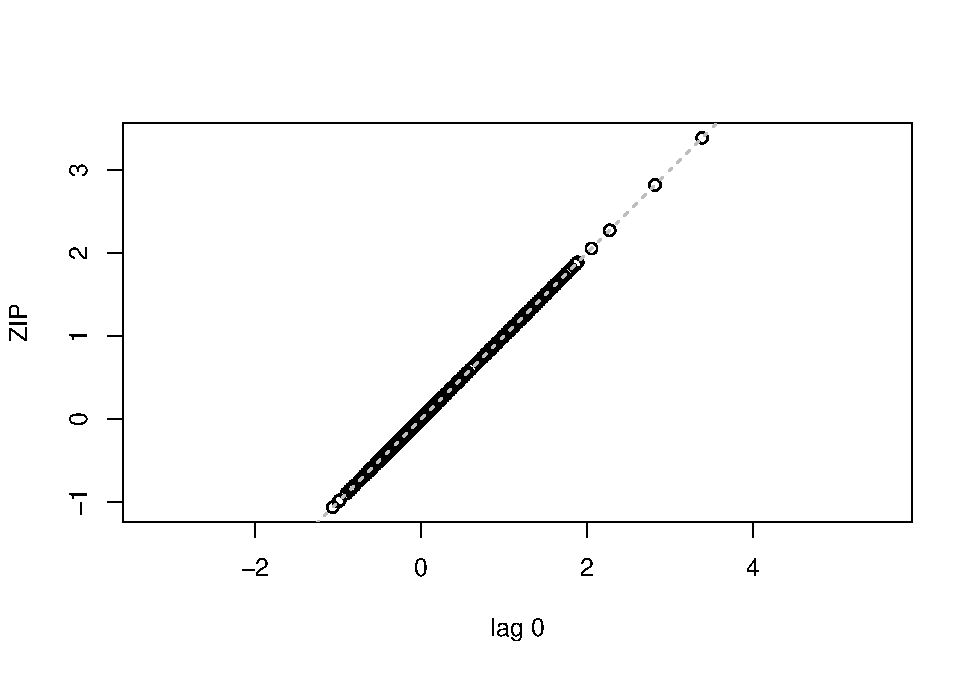
\includegraphics{LongPanelDataScripts_files/figure-latex/unnamed-chunk-48-5.pdf} 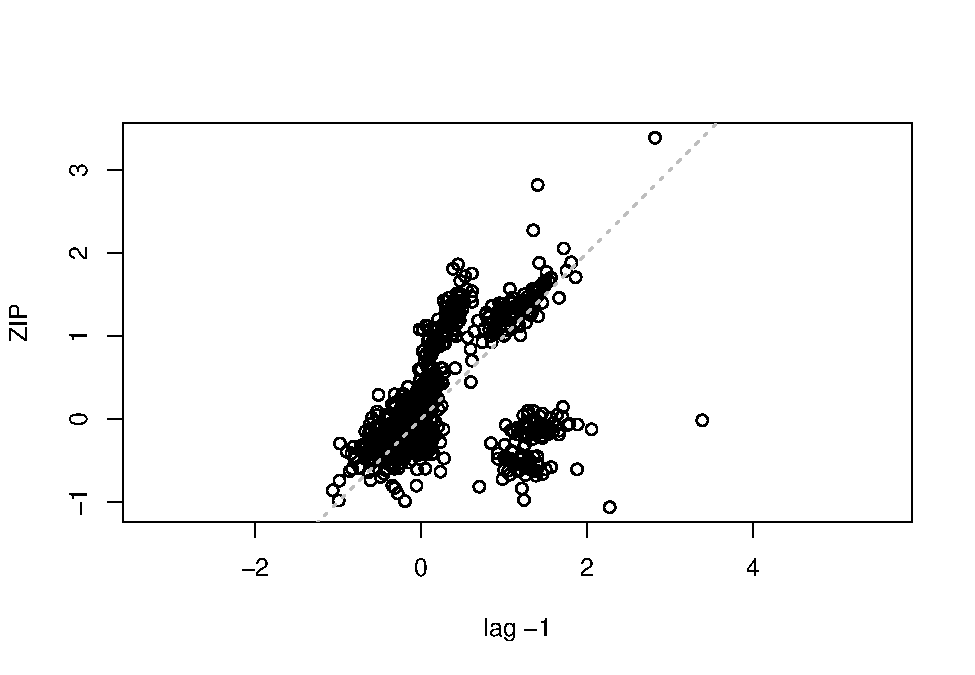
\includegraphics{LongPanelDataScripts_files/figure-latex/unnamed-chunk-48-6.pdf}

\hypertarget{model-3.-error-components-model-with-autocorrelated-errors}{%
\subsection{MODEL 3. Error components model with autocorrelated errors}\label{model-3.-error-components-model-with-autocorrelated-errors}}

\begin{Shaded}
\begin{Highlighting}[]
\NormalTok{lme2<-}\KeywordTok{update}\NormalTok{(lme1, }\DataTypeTok{correlation=}\KeywordTok{corAR1}\NormalTok{(}\DataTypeTok{form=}\OperatorTok{~}\NormalTok{TIME}\OperatorTok{|}\NormalTok{ZIP))}
\KeywordTok{summary}\NormalTok{(lme2)}
\end{Highlighting}
\end{Shaded}

\begin{verbatim}
Linear mixed-effects model fit by REML
 Data: Lottery2 
       AIC      BIC    logLik
  2318.834 2389.835 -1146.417

Random effects:
 Formula: ~1 | ZIP
        (Intercept)  Residual
StdDev:    0.726541 0.5282642

Correlation Structure: AR(1)
 Formula: ~TIME | ZIP 
 Parameter estimate(s):
      Phi 
0.5552575 
Fixed effects: LNSALES ~ PERPERHH + MEDSCHYR + MEDHVL + PRCRENT + PRC55P + HHMEDAGE +      MEDINC + POPULATN + NRETAIL 
                Value Std.Error   DF    t-value p-value
(Intercept) 15.254535  7.005477 1699  2.1775157  0.0296
PERPERHH    -1.149312  0.842554   41 -1.3640808  0.1800
MEDSCHYR    -0.911242  0.360225   41 -2.5296504  0.0154
MEDHVL       0.011273  0.013960   41  0.8074825  0.4240
PRCRENT      0.030104  0.019652   41  1.5319015  0.1332
PRC55P      -0.071434  0.070515   41 -1.0130333  0.3170
HHMEDAGE     0.119779  0.110336   41  1.0855851  0.2840
MEDINC       0.044082  0.027916   41  1.5790867  0.1220
POPULATN     0.080430  0.029449   41  2.7311900  0.0093
NRETAIL      0.003887  0.019402 1699  0.2003424  0.8412
 Correlation: 
         (Intr) PERPER MEDSCH MEDHVL PRCREN PRC55P HHMEDA MEDINC POPULA
PERPERHH -0.632                                                        
MEDSCHYR -0.750  0.209                                                 
MEDHVL    0.286  0.097 -0.373                                          
PRCRENT  -0.204  0.403 -0.246  0.014                                   
PRC55P    0.144  0.236 -0.017  0.069  0.039                            
HHMEDAGE -0.457  0.049  0.108 -0.128  0.151 -0.898                     
MEDINC   -0.167 -0.014  0.077 -0.652  0.212  0.392 -0.200              
POPULATN  0.217 -0.042 -0.269 -0.196 -0.281 -0.035  0.032 -0.037       
NRETAIL  -0.245  0.097  0.285  0.185  0.112  0.017 -0.002 -0.031 -0.881

Standardized Within-Group Residuals:
        Min          Q1         Med          Q3         Max 
-1.87105785 -0.46121477 -0.26278521  0.04905521  6.55032232 

Number of Observations: 1750
Number of Groups: 50 
\end{verbatim}

\hypertarget{model-4.-more-parsimonious-random-effects-model}{%
\subsection{MODEL 4. More parsimonious random effects model}\label{model-4.-more-parsimonious-random-effects-model}}

\begin{Shaded}
\begin{Highlighting}[]
\NormalTok{lme3<-}\KeywordTok{lme}\NormalTok{(LNSALES}\OperatorTok{~}\NormalTok{MEDSCHYR}\OperatorTok{+}\NormalTok{POPULATN, }\DataTypeTok{data=}\NormalTok{Lottery2, }\DataTypeTok{random=}\OperatorTok{~}\DecValTok{1}\OperatorTok{|}\NormalTok{ZIP, }\DataTypeTok{correlation=}\KeywordTok{corAR1}\NormalTok{(}\DataTypeTok{form=}\OperatorTok{~}\NormalTok{TIME}\OperatorTok{|}\NormalTok{ZIP))}
\KeywordTok{summary}\NormalTok{(lme3)}
\end{Highlighting}
\end{Shaded}

\begin{verbatim}
Linear mixed-effects model fit by REML
 Data: Lottery2 
       AIC      BIC    logLik
  2291.584 2324.378 -1139.792

Random effects:
 Formula: ~1 | ZIP
        (Intercept)  Residual
StdDev:    0.838855 0.5280303

Correlation Structure: AR(1)
 Formula: ~TIME | ZIP 
 Parameter estimate(s):
      Phi 
0.5549028 
Fixed effects: LNSALES ~ MEDSCHYR + POPULATN 
                Value Std.Error   DF   t-value p-value
(Intercept)  7.983814  3.407381 1700  2.343094  0.0192
MEDSCHYR    -0.097917  0.273978   47 -0.357391  0.7224
POPULATN     0.108468  0.013613   47  7.968097  0.0000
 Correlation: 
         (Intr) MEDSCH
MEDSCHYR -0.999       
POPULATN  0.565 -0.590

Standardized Within-Group Residuals:
        Min          Q1         Med          Q3         Max 
-1.81585940 -0.45547600 -0.25704219  0.06499433  6.60925098 

Number of Observations: 1750
Number of Groups: 50 
\end{verbatim}

\begin{Shaded}
\begin{Highlighting}[]
\CommentTok{#THE POOLED CROSS-SECTIONAL MODEL WITH AUTOCORRELATED ERRORS}
\CommentTok{#Default method for gls is reml, gls can be viewed as an lme function without the argument random}
\NormalTok{gls1<-}\KeywordTok{gls}\NormalTok{(LNSALES}\OperatorTok{~}\NormalTok{PERPERHH}\OperatorTok{+}\NormalTok{MEDSCHYR}\OperatorTok{+}\NormalTok{MEDHVL}\OperatorTok{+}\NormalTok{PRCRENT}\OperatorTok{+}\NormalTok{PRC55P}\OperatorTok{+}\NormalTok{HHMEDAGE}\OperatorTok{+}\NormalTok{MEDINC}\OperatorTok{+}\NormalTok{POPULATN}\OperatorTok{+}\NormalTok{NRETAIL, }\DataTypeTok{data=}\NormalTok{Lottery2, }\DataTypeTok{correlation=}\KeywordTok{corAR1}\NormalTok{(}\DataTypeTok{form=}\OperatorTok{~}\NormalTok{TIME}\OperatorTok{|}\NormalTok{ZIP)) }
\NormalTok{gls1}
\end{Highlighting}
\end{Shaded}

\begin{verbatim}
Generalized least squares fit by REML
  Model: LNSALES ~ PERPERHH + MEDSCHYR + MEDHVL + PRCRENT + PRC55P + HHMEDAGE +      MEDINC + POPULATN + NRETAIL 
  Data: Lottery2 
  Log-restricted-likelihood: -1240.823

Coefficients:
(Intercept)    PERPERHH    MEDSCHYR      MEDHVL     PRCRENT      PRC55P 
13.59613280 -1.06322470 -0.82003019  0.01293351  0.03252353 -0.07218282 
   HHMEDAGE      MEDINC    POPULATN     NRETAIL 
 0.12285161  0.04322324  0.05898877  0.02014254 

Correlation Structure: AR(1)
 Formula: ~TIME | ZIP 
 Parameter estimate(s):
      Phi 
0.8240088 
Degrees of freedom: 1750 total; 1740 residual
Residual standard error: 0.8427768 
\end{verbatim}

\hypertarget{model-5.-fixed-effects-model-with-autocorrelated-errors}{%
\subsection{MODEL 5. Fixed effects model with autocorrelated errors}\label{model-5.-fixed-effects-model-with-autocorrelated-errors}}

\begin{Shaded}
\begin{Highlighting}[]
\NormalTok{Lottery2}\OperatorTok{$}\NormalTok{ZIPfac=}\KeywordTok{factor}\NormalTok{(Lottery2}\OperatorTok{$}\NormalTok{ZIP)}
\NormalTok{gls2<-}\KeywordTok{gls}\NormalTok{(LNSALES}\OperatorTok{~}\NormalTok{ZIPfac, }\DataTypeTok{data=}\NormalTok{Lottery2, }\DataTypeTok{correlation=}\KeywordTok{corAR1}\NormalTok{(}\DataTypeTok{form=}\OperatorTok{~}\NormalTok{TIME}\OperatorTok{|}\NormalTok{ZIPfac)) }
\NormalTok{gls2}
\end{Highlighting}
\end{Shaded}

\begin{verbatim}
Generalized least squares fit by REML
  Model: LNSALES ~ ZIPfac 
  Data: Lottery2 
  Log-restricted-likelihood: -1073.063

Coefficients:
(Intercept) ZIPfac53033 ZIPfac53038 ZIPfac53059 ZIPfac53072 ZIPfac53083 
 7.02034302  1.07644720  0.61877604 -0.01329196  2.45963633  1.97648544 
ZIPfac53095 ZIPfac53098 ZIPfac53104 ZIPfac53172 ZIPfac53211 ZIPfac53520 
 3.27341024  0.59051473  2.12004892  2.56764964  2.68989060  1.53954270 
ZIPfac53544 ZIPfac53563 ZIPfac53572 ZIPfac53574 ZIPfac53813 ZIPfac53924 
-1.22340317  1.68388653  0.81336415  0.64605315  0.79960910 -1.46385511 
ZIPfac53934 ZIPfac53943 ZIPfac53952 ZIPfac54115 ZIPfac54143 ZIPfac54153 
 0.65471544 -1.31041280  0.49735851  2.03324306  2.40463509  1.12075652 
ZIPfac54170 ZIPfac54205 ZIPfac54213 ZIPfac54220 ZIPfac54235 ZIPfac54241 
-0.09585752 -0.80190426 -0.69482488  3.22278219  2.21634671  1.96067334 
ZIPfac54302 ZIPfac54406 ZIPfac54436 ZIPfac54457 ZIPfac54470 ZIPfac54474 
 2.39541360  0.75120386 -1.31334267  1.60733345 -0.28003078  0.51088577 
ZIPfac54480 ZIPfac54531 ZIPfac54556 ZIPfac54614 ZIPfac54622 ZIPfac54634 
-1.62581025 -0.73327749 -0.37613230 -0.50434660 -0.79801244  0.49941189 
ZIPfac54650 ZIPfac54701 ZIPfac54724 ZIPfac54745 ZIPfac54758 ZIPfac54810 
 2.50724987  2.72121016  0.66159018 -0.99678783  0.71914194 -1.16821041 
ZIPfac54839 ZIPfac54956 
-2.00207902  2.57602144 

Correlation Structure: AR(1)
 Formula: ~TIME | ZIPfac 
 Parameter estimate(s):
    Phi 
0.55476 
Degrees of freedom: 1750 total; 1700 residual
Residual standard error: 0.5279669 
\end{verbatim}

\begin{Shaded}
\begin{Highlighting}[]
\CommentTok{# Note the difference between R estimates and SAS estimates is because in SAS the estimate }
\CommentTok{# for ZIP 54956 is restricted to be zero, in R the intercept and estimates for Zip are }
\CommentTok{# scaled differently, but both estimates should give us approximately the same answer#}
\end{Highlighting}
\end{Shaded}

The five models listed are summarized in Table 4.4 at Page 146.

\hypertarget{multilevel-models}{%
\chapter{Multilevel Models}\label{multilevel-models}}

\hypertarget{import-data-4}{%
\section{Import Data}\label{import-data-4}}

\begin{Shaded}
\begin{Highlighting}[]
\CommentTok{#Dental=read.table(choose.files(), header=TRUE, sep="\textbackslash{}t")}
\CommentTok{#library(mice)}
\CommentTok{#data(potthoffroy)}
\CommentTok{# I make this dataset myself according to data(potthoffroy)}
\NormalTok{Dental <-}\StringTok{ }\KeywordTok{read.table}\NormalTok{(}\StringTok{"TXTData/dental.txt"}\NormalTok{,}\DataTypeTok{sep =}\StringTok{"}\CharTok{\textbackslash{}t}\StringTok{"}\NormalTok{, }\DataTypeTok{quote =} \StringTok{""}\NormalTok{, }\DataTypeTok{header=}\OtherTok{TRUE}\NormalTok{)}

\KeywordTok{names}\NormalTok{(Dental)<-}\KeywordTok{c}\NormalTok{(}\StringTok{"MEASURE"}\NormalTok{, }\StringTok{"SEX"}\NormalTok{, }\StringTok{"AGE"}\NormalTok{, }\StringTok{"ID"}\NormalTok{)}
\end{Highlighting}
\end{Shaded}

\hypertarget{example-5.2-dental-data-page-175}{%
\section{Example 5.2: Dental Data (Page 175)}\label{example-5.2-dental-data-page-175}}

This example is originally due to Potthoff and Roy (1964B); see also Rao (1987B). Here, y is the distance, measured in millimeters, from the center of the pituitary to the pteryomaxillary fissure. Measurements were taken on eleven girls and sixteen boys at ages 8, 10, 12, and 14. Of interest is the relation between the distance and age, specifically, in how the distance grows with age and whether there is a difference between males and females.

\hypertarget{figure-5.1.-multiple-time-series-plot}{%
\subsection{Figure 5.1. Multiple time series plot}\label{figure-5.1.-multiple-time-series-plot}}

\begin{Shaded}
\begin{Highlighting}[]
\KeywordTok{plot}\NormalTok{(MEASURE }\OperatorTok{~}\StringTok{ }\NormalTok{AGE, }\DataTypeTok{data =}\NormalTok{ Dental, }\DataTypeTok{xlab=}\StringTok{""}\NormalTok{, }\DataTypeTok{ylab=}\StringTok{""}\NormalTok{, }\DataTypeTok{xaxt=}\StringTok{"n"}\NormalTok{, }\DataTypeTok{yaxt=}\StringTok{"n"}\NormalTok{)}
 \ControlFlowTok{for}\NormalTok{ (i }\ControlFlowTok{in}\NormalTok{ Dental}\OperatorTok{$}\NormalTok{ID) \{}
 \KeywordTok{lines}\NormalTok{(MEASURE }\OperatorTok{~}\StringTok{ }\NormalTok{AGE, }\DataTypeTok{data =} \KeywordTok{subset}\NormalTok{(Dental, ID }\OperatorTok{==}\StringTok{ }\NormalTok{i)) \}}

\KeywordTok{axis}\NormalTok{(}\DecValTok{2}\NormalTok{, }\DataTypeTok{at=}\KeywordTok{seq}\NormalTok{(}\DecValTok{16}\NormalTok{, }\DecValTok{32}\NormalTok{, }\DataTypeTok{by=}\DecValTok{2}\NormalTok{), }\DataTypeTok{las=}\DecValTok{1}\NormalTok{, }\DataTypeTok{font=}\DecValTok{10}\NormalTok{, }\DataTypeTok{cex=}\FloatTok{0.005}\NormalTok{, }\DataTypeTok{tck=}\FloatTok{0.01}\NormalTok{)}
\KeywordTok{axis}\NormalTok{(}\DecValTok{2}\NormalTok{, }\DataTypeTok{at=}\KeywordTok{seq}\NormalTok{(}\DecValTok{16}\NormalTok{, }\DecValTok{32}\NormalTok{, }\DataTypeTok{by=}\DecValTok{1}\NormalTok{), }\DataTypeTok{lab=}\NormalTok{F, }\DataTypeTok{tck=}\FloatTok{0.005}\NormalTok{)}
\KeywordTok{axis}\NormalTok{(}\DecValTok{1}\NormalTok{, }\DataTypeTok{at=}\KeywordTok{seq}\NormalTok{(}\DecValTok{8}\NormalTok{,}\DecValTok{14}\NormalTok{, }\DataTypeTok{by=}\DecValTok{2}\NormalTok{), }\DataTypeTok{font=}\DecValTok{10}\NormalTok{, }\DataTypeTok{cex=}\FloatTok{0.005}\NormalTok{, }\DataTypeTok{tck=}\FloatTok{0.01}\NormalTok{)}
\KeywordTok{axis}\NormalTok{(}\DecValTok{1}\NormalTok{, }\DataTypeTok{at=}\KeywordTok{seq}\NormalTok{(}\DecValTok{8}\NormalTok{,}\DecValTok{14}\NormalTok{, }\DataTypeTok{by=}\FloatTok{0.2}\NormalTok{), }\DataTypeTok{lab=}\NormalTok{F, }\DataTypeTok{tck=}\FloatTok{0.005}\NormalTok{)}
\KeywordTok{mtext}\NormalTok{(}\StringTok{"MEASURE"}\NormalTok{, }\DataTypeTok{side=}\DecValTok{2}\NormalTok{, }\DataTypeTok{line=}\OperatorTok{-}\DecValTok{2}\NormalTok{, }\DataTypeTok{at=}\FloatTok{32.5}\NormalTok{, }\DataTypeTok{font=}\DecValTok{10}\NormalTok{, }\DataTypeTok{cex=}\DecValTok{1}\NormalTok{, }\DataTypeTok{las=}\DecValTok{1}\NormalTok{)}
\KeywordTok{mtext}\NormalTok{(}\StringTok{"AGE"}\NormalTok{, }\DataTypeTok{side=}\DecValTok{1}\NormalTok{, }\DataTypeTok{line=}\DecValTok{2}\NormalTok{, }\DataTypeTok{at=}\DecValTok{11}\NormalTok{, }\DataTypeTok{font=}\DecValTok{10}\NormalTok{, }\DataTypeTok{cex=}\DecValTok{1}\NormalTok{, }\DataTypeTok{las=}\DecValTok{1}\NormalTok{)}
\end{Highlighting}
\end{Shaded}

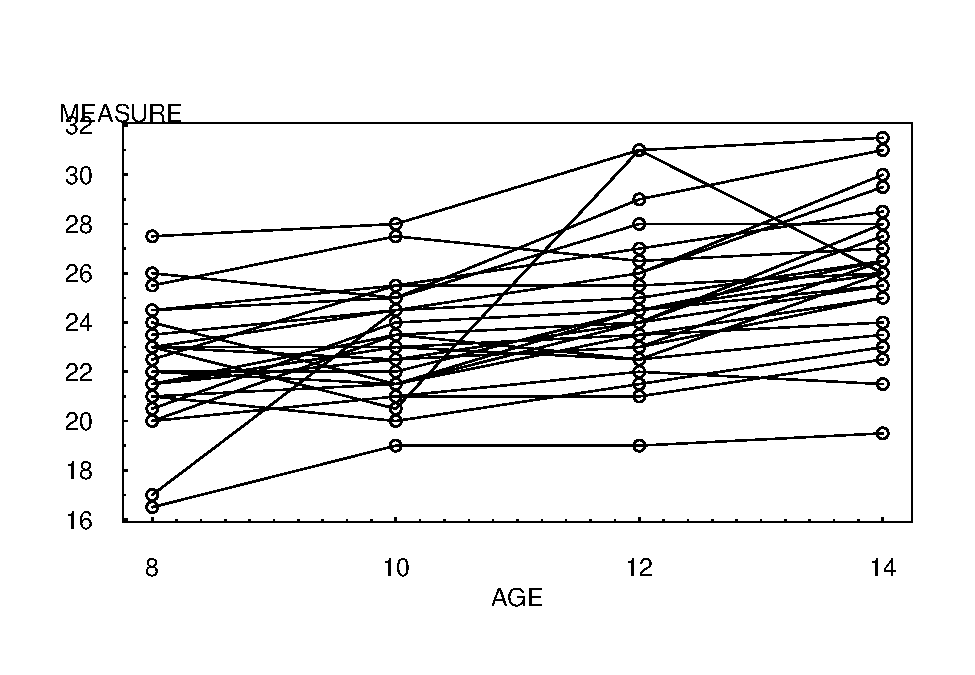
\includegraphics{LongPanelDataScripts_files/figure-latex/unnamed-chunk-54-1.pdf}

From Figure 5.1, we can see that the measurement length grows as each child ages, although it is difficult to detect differences between boys and girls. In Figure 5.1, we use open circular plotting symbols for girls and filled circular plotting symbols for boys. Figure 5.1 does show that the ninth boy has an unusual growth pattern; this pattern can also be seen in Table 5.1.

\hypertarget{summary-statistics}{%
\subsection{Summary statistics}\label{summary-statistics}}

\begin{Shaded}
\begin{Highlighting}[]
\KeywordTok{summary}\NormalTok{(Dental[, }\KeywordTok{c}\NormalTok{(}\StringTok{"MEASURE"}\NormalTok{)])}
\end{Highlighting}
\end{Shaded}

\begin{verbatim}
   Min. 1st Qu.  Median    Mean 3rd Qu.    Max. 
  16.50   22.00   23.75   24.02   26.00   31.50 
\end{verbatim}

\hypertarget{trellis-plot-unique-in-r}{%
\subsection{Trellis plot, unique in r}\label{trellis-plot-unique-in-r}}

\begin{Shaded}
\begin{Highlighting}[]
\NormalTok{dent1 =}\StringTok{ }\KeywordTok{groupedData}\NormalTok{(MEASURE }\OperatorTok{~}\StringTok{ }\NormalTok{AGE }\OperatorTok{|}\StringTok{ }\NormalTok{ID, }\DataTypeTok{data=}\NormalTok{Dental, }\DataTypeTok{outer=}\OperatorTok{~}\NormalTok{SEX)}
\KeywordTok{plot}\NormalTok{(dent1, }\DataTypeTok{layout =} \KeywordTok{c}\NormalTok{(}\DecValTok{16}\NormalTok{,}\DecValTok{2}\NormalTok{))}
\end{Highlighting}
\end{Shaded}

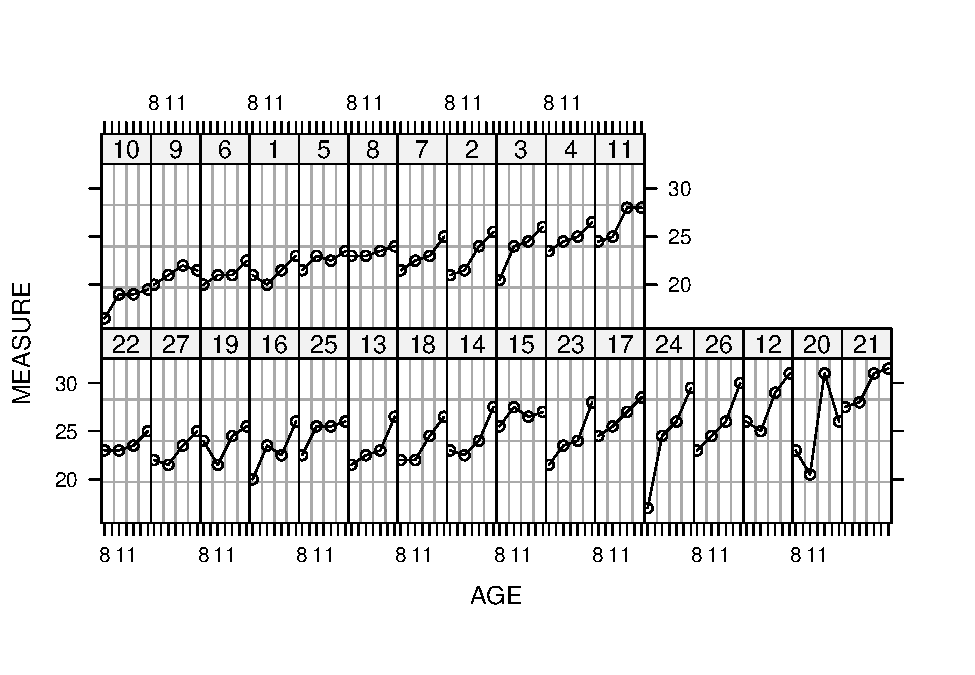
\includegraphics{LongPanelDataScripts_files/figure-latex/unnamed-chunk-56-1.pdf}

\hypertarget{table-5.2-dental-data-growth-curve-model-parameter-estimates}{%
\section{TABLE 5.2: Dental data growth-curve-model parameter estimates}\label{table-5.2-dental-data-growth-curve-model-parameter-estimates}}

\hypertarget{table-5.2-error-components-model}{%
\subsection{TABLE 5.2: Error components model}\label{table-5.2-error-components-model}}

\begin{Shaded}
\begin{Highlighting}[]
\NormalTok{dental1.lme<-}\KeywordTok{lme}\NormalTok{(MEASURE}\OperatorTok{~}\NormalTok{AGE}\OperatorTok{*}\NormalTok{SEX, }\DataTypeTok{data=}\NormalTok{Dental, }\DataTypeTok{random=}\OperatorTok{~}\DecValTok{1}\OperatorTok{|}\NormalTok{ID)}
\KeywordTok{summary}\NormalTok{(dental1.lme)}
\end{Highlighting}
\end{Shaded}

\begin{verbatim}
Linear mixed-effects model fit by REML
 Data: Dental 
       AIC      BIC    logLik
  445.7572 461.6236 -216.8786

Random effects:
 Formula: ~1 | ID
        (Intercept) Residual
StdDev:    1.816214 1.386382

Fixed effects: MEASURE ~ AGE * SEX 
                Value Std.Error DF   t-value p-value
(Intercept) 16.340625 0.9813122 79 16.651810  0.0000
AGE          0.784375 0.0775011 79 10.120823  0.0000
SEX          1.032102 1.5374208 25  0.671321  0.5082
AGE:SEX     -0.304830 0.1214209 79 -2.510520  0.0141
 Correlation: 
        (Intr) AGE    SEX   
AGE     -0.869              
SEX     -0.638  0.555       
AGE:SEX  0.555 -0.638 -0.869

Standardized Within-Group Residuals:
        Min          Q1         Med          Q3         Max 
-3.59804400 -0.45461690  0.01578365  0.50244658  3.68620792 

Number of Observations: 108
Number of Groups: 27 
\end{verbatim}

\hypertarget{table-5.2-growth-curve-model}{%
\subsection{TABLE 5.2: Growth curve model}\label{table-5.2-growth-curve-model}}

\begin{Shaded}
\begin{Highlighting}[]
\NormalTok{dental2.lme<-}\KeywordTok{lme}\NormalTok{(MEASURE}\OperatorTok{~}\NormalTok{AGE}\OperatorTok{*}\NormalTok{SEX, }\DataTypeTok{data=}\NormalTok{Dental, }\DataTypeTok{random=}\OperatorTok{~}\DecValTok{1}\OperatorTok{+}\NormalTok{AGE}\OperatorTok{|}\NormalTok{ID, }\DataTypeTok{correlation=}\KeywordTok{corSymm}\NormalTok{(}\DataTypeTok{form=}\OperatorTok{~}\DecValTok{1}\OperatorTok{|}\NormalTok{ID),}\DataTypeTok{control=} \KeywordTok{lmeControl}\NormalTok{(}\DataTypeTok{opt =} \StringTok{"optim"}\NormalTok{)) }\CommentTok{# I add the code "control= lmeControl(opt = "optim")" to fix converge problem}
\CommentTok{#corSymm gives a general correlation structure in lme}
\NormalTok{dental2.lme}
\end{Highlighting}
\end{Shaded}

\begin{verbatim}
Linear mixed-effects model fit by REML
  Data: Dental 
  Log-restricted-likelihood: -213.0644
  Fixed: MEASURE ~ AGE * SEX 
(Intercept)         AGE         SEX     AGE:SEX 
 15.9304961   0.8243798   1.4779148  -0.3483069 

Random effects:
 Formula: ~1 + AGE | ID
 Structure: General positive-definite, Log-Cholesky parametrization
            StdDev     Corr  
(Intercept) 1.73852535 (Intr)
AGE         0.07167425 -0.238
Residual    1.49360182       

Correlation Structure: General
 Formula: ~1 | ID 
 Parameter estimate(s):
 Correlation: 
  1      2      3     
2  0.015              
3  0.172  0.017       
4 -0.111  0.431  0.341
Number of Observations: 108
Number of Groups: 27 
\end{verbatim}

\hypertarget{table-5.2-growth-curve-model---omitting-9th-boy}{%
\subsection{TABLE 5.2: Growth curve model - omitting 9th boy}\label{table-5.2-growth-curve-model---omitting-9th-boy}}

\begin{Shaded}
\begin{Highlighting}[]
\NormalTok{Dental2<-}\KeywordTok{subset}\NormalTok{(Dental, ID}\OperatorTok{!=}\DecValTok{20}\NormalTok{)}
\NormalTok{dental3.lme<-}\KeywordTok{update}\NormalTok{(dental2.lme, }\DataTypeTok{data=}\NormalTok{Dental2)}
\NormalTok{dental3.lme}
\end{Highlighting}
\end{Shaded}

\begin{verbatim}
Linear mixed-effects model fit by REML
  Data: Dental2 
  Log-restricted-likelihood: -188.7711
  Fixed: MEASURE ~ AGE * SEX 
(Intercept)         AGE         SEX     AGE:SEX 
 16.8586091   0.7699492   0.6119536  -0.2975491 

Random effects:
 Formula: ~1 + AGE | ID
 Structure: General positive-definite, Log-Cholesky parametrization
            StdDev     Corr  
(Intercept) 1.63375372 (Intr)
AGE         0.06425145 0.028 
Residual    1.28363690       

Correlation Structure: General
 Formula: ~1 | ID 
 Parameter estimate(s):
 Correlation: 
  1      2      3     
2 -0.200              
3  0.080  0.518       
4 -0.511  0.169  0.562
Number of Observations: 104
Number of Groups: 26 
\end{verbatim}

Table 5.2 shows the parameter estimates for this model. Here, we see that the coefficient associated with linear growth is statistically significant, over all models. Moreover, the rate of increase for girls is lower than for boys. The estimated covariance between \(\alpha_{0i}\) and \(\alpha_{1i}\) (which is also the estimated covariance between \(\beta_{0i}\) and \(β_{1i}\) turns out to be negative. One interpretation of the negative covariance between initial status and growth rate is that subjects who start at a low level tend to grow more quickly than those who start at higher levels, and vice versa.

For comparison purposes, Table 5.2 shows the parameter estimates with the ninth boy deleted. The effects of this subject deletion on the parameter estimates are small. Table 5.2 also shows parameter estimates of the errorcomponents model. This model employs the same level-1 model but with level-2 models

\[\beta_{0i}=\beta_{00}+\beta_{01} \text{GENDER}_i + \alpha_{0i}\]

\[\beta_{1i}=\beta_{10}+\beta_{11} \text{GENDER}_i\]
With parameter estimates calculated using the full data set, there again is little change in the parameter estimates. Because the results appear to be robust to both unusual subjects and model selection, we have greater confidence in our interpretations.

\hypertarget{modeling-issues}{%
\chapter{Modeling Issues}\label{modeling-issues}}

\hypertarget{import-data-5}{%
\section{Import Data}\label{import-data-5}}

\begin{Shaded}
\begin{Highlighting}[]
\NormalTok{taxprep=}\KeywordTok{read.table}\NormalTok{(}\StringTok{"TXTData/TaxPrep.txt"}\NormalTok{, }\DataTypeTok{sep =}\StringTok{"}\CharTok{\textbackslash{}t}\StringTok{"}\NormalTok{, }\DataTypeTok{quote =} \StringTok{""}\NormalTok{,}\DataTypeTok{header=}\OtherTok{TRUE}\NormalTok{)}

\CommentTok{#taxprep=read.table(choose.files(), header=TRUE, sep="\textbackslash{}t")}
\end{Highlighting}
\end{Shaded}

Data for this study are from the Statistics of Income (SOI) Panel of Individual Returns, a part of the Ernst and Young/University of Michigan Tax Research Database. The SOI Panel represents a simple random sample of unaudited individual income tax returns filed for tax years 1979-1990. The data are compiled from a stratified probability sample of unaudited individual income tax returns, Forms 1040, 1040A and 1040EZ, filed by U.S. taxpayers. The estimates that are obtained from these data are intended to represent all returns filed for the income tax years under review. All returns processed are subjected to sampling except tentative and amended returns.

\begin{longtable}[]{@{}ll@{}}
\toprule
\begin{minipage}[b]{0.54\columnwidth}\raggedright
Variable\strut
\end{minipage} & \begin{minipage}[b]{0.40\columnwidth}\raggedright
Description\strut
\end{minipage}\tabularnewline
\midrule
\endhead
\begin{minipage}[t]{0.54\columnwidth}\raggedright
MS\strut
\end{minipage} & \begin{minipage}[t]{0.40\columnwidth}\raggedright
is an indicator variable of the taxpayer's marital status. It is coded one if the taxpayer is married and zero otherwise.\strut
\end{minipage}\tabularnewline
\begin{minipage}[t]{0.54\columnwidth}\raggedright
HH\strut
\end{minipage} & \begin{minipage}[t]{0.40\columnwidth}\raggedright
is an indicator variable, one if the taxpayer is a head of household and zero otherwise.\strut
\end{minipage}\tabularnewline
\begin{minipage}[t]{0.54\columnwidth}\raggedright
DEPEND\strut
\end{minipage} & \begin{minipage}[t]{0.40\columnwidth}\raggedright
is the number of dependents claimed by the taxpayer.\strut
\end{minipage}\tabularnewline
\begin{minipage}[t]{0.54\columnwidth}\raggedright
AGE\strut
\end{minipage} & \begin{minipage}[t]{0.40\columnwidth}\raggedright
is the presence of an indicator for age 65 or over.\strut
\end{minipage}\tabularnewline
\begin{minipage}[t]{0.54\columnwidth}\raggedright
F1040A\strut
\end{minipage} & \begin{minipage}[t]{0.40\columnwidth}\raggedright
is an indicator variable of the taxpayer's filing type. It is coded one if the taxpayer uses Form 1040A and zero otherwise.\strut
\end{minipage}\tabularnewline
\begin{minipage}[t]{0.54\columnwidth}\raggedright
F1040EZ\strut
\end{minipage} & \begin{minipage}[t]{0.40\columnwidth}\raggedright
is an indicator variable of the taxpayer's filing type. It is coded one if the taxpayer uses Form 1040EZ and zero otherwise.\strut
\end{minipage}\tabularnewline
\begin{minipage}[t]{0.54\columnwidth}\raggedright
TPI\strut
\end{minipage} & \begin{minipage}[t]{0.40\columnwidth}\raggedright
is the sum of all positive income line items on the return.\strut
\end{minipage}\tabularnewline
\begin{minipage}[t]{0.54\columnwidth}\raggedright
TXRT\strut
\end{minipage} & \begin{minipage}[t]{0.40\columnwidth}\raggedright
is a marginal tax rate. It is computed on TPI less exemptions and the standard deduction.\strut
\end{minipage}\tabularnewline
\begin{minipage}[t]{0.54\columnwidth}\raggedright
MR\strut
\end{minipage} & \begin{minipage}[t]{0.40\columnwidth}\raggedright
is an exogenous marginal tax rate. It is computed on TPI less exemptions and the standard deduction.\strut
\end{minipage}\tabularnewline
\begin{minipage}[t]{0.54\columnwidth}\raggedright
EMP\strut
\end{minipage} & \begin{minipage}[t]{0.40\columnwidth}\raggedright
is an indicator variable, one if Schedule C or F is present and zero otherwise. Self-employed taxpayers have greater need for professional assistance to reduce the reporting risks of doing business.\strut
\end{minipage}\tabularnewline
\begin{minipage}[t]{0.54\columnwidth}\raggedright
PREP\strut
\end{minipage} & \begin{minipage}[t]{0.40\columnwidth}\raggedright
is a variable indicating the presence of a paid preparer.\strut
\end{minipage}\tabularnewline
\begin{minipage}[t]{0.54\columnwidth}\raggedright
TAX\strut
\end{minipage} & \begin{minipage}[t]{0.40\columnwidth}\raggedright
is the tax liability on the return.\strut
\end{minipage}\tabularnewline
\begin{minipage}[t]{0.54\columnwidth}\raggedright
SUBJECT\strut
\end{minipage} & \begin{minipage}[t]{0.40\columnwidth}\raggedright
Subject identifier, 1-258.\strut
\end{minipage}\tabularnewline
\begin{minipage}[t]{0.54\columnwidth}\raggedright
TIME\strut
\end{minipage} & \begin{minipage}[t]{0.40\columnwidth}\raggedright
Time identifier, 1-5.\strut
\end{minipage}\tabularnewline
\begin{minipage}[t]{0.54\columnwidth}\raggedright
LNTAX\strut
\end{minipage} & \begin{minipage}[t]{0.40\columnwidth}\raggedright
is the natural logarithm of the tax liability on the return.\strut
\end{minipage}\tabularnewline
\begin{minipage}[t]{0.54\columnwidth}\raggedright
LNTPI\strut
\end{minipage} & \begin{minipage}[t]{0.40\columnwidth}\raggedright
is the natural logarithm of the sum of all positive income line items on the return.\strut
\end{minipage}\tabularnewline
\bottomrule
\end{longtable}

\hypertarget{example-7.2-income-tax-payments-page-248}{%
\section{Example 7.2: Income Tax Payments (Page 248)}\label{example-7.2-income-tax-payments-page-248}}

To illustrate the performance of the fixed-effects estimators and omitted-variable tests, we examine data on determinants of income tax payments introduced in Section 3.2. Specifically, we begin with the error-components model with K = 8 coefficients estimated using generalized least squares.

\hypertarget{table-7.1-fixed-effects-estimators}{%
\subsection{TABLE 7.1: Fixed effects estimators}\label{table-7.1-fixed-effects-estimators}}

\begin{Shaded}
\begin{Highlighting}[]
\NormalTok{taxprep}\OperatorTok{$}\NormalTok{YEAR<-taxprep}\OperatorTok{$}\NormalTok{TIME}\OperatorTok{+}\DecValTok{1981}
\NormalTok{taxprep}\OperatorTok{$}\NormalTok{SUBFACTOR<-}\KeywordTok{factor}\NormalTok{(taxprep}\OperatorTok{$}\NormalTok{SUBJECT)}
\KeywordTok{library}\NormalTok{(nlme)}
\NormalTok{taxprepfx<-}\KeywordTok{lm}\NormalTok{(LNTAX}\OperatorTok{~}\NormalTok{MS}\OperatorTok{+}\NormalTok{HH}\OperatorTok{+}\NormalTok{AGE}\OperatorTok{+}\NormalTok{EMP}\OperatorTok{+}\NormalTok{PREP}\OperatorTok{+}\NormalTok{LNTPI}\OperatorTok{+}\NormalTok{DEPEND}\OperatorTok{+}\NormalTok{MR}\OperatorTok{+}\NormalTok{SUBFACTOR}\DecValTok{-1}\NormalTok{, }\DataTypeTok{data=}\NormalTok{taxprep) }
\KeywordTok{summary}\NormalTok{(taxprepfx)}
\end{Highlighting}
\end{Shaded}

\begin{verbatim}

Call:
lm(formula = LNTAX ~ MS + HH + AGE + EMP + PREP + LNTPI + DEPEND + 
    MR + SUBFACTOR - 1, data = taxprep)

Residuals:
    Min      1Q  Median      3Q     Max 
-7.4350 -0.3315 -0.0078  0.4586  6.9348 

Coefficients:
              Estimate Std. Error t value Pr(>|t|)    
MS            0.072328   0.255221   0.283 0.776933    
HH           -0.706799   0.326079  -2.168 0.030421 *  
AGE           0.001840   0.322918   0.006 0.995456    
EMP          -0.244247   0.247434  -0.987 0.323817    
PREP         -0.029685   0.163207  -0.182 0.855707    
LNTPI         0.716755   0.077101   9.296  < 2e-16 ***
DEPEND       -0.069021   0.082707  -0.835 0.404184    
MR            0.121920   0.008998  13.550  < 2e-16 ***
SUBFACTOR1   -1.941454   0.912856  -2.127 0.033676 *  
SUBFACTOR2   -2.076922   0.921470  -2.254 0.024412 *  
SUBFACTOR3   -3.762761   0.867812  -4.336 1.59e-05 ***
SUBFACTOR4   -2.390221   0.936929  -2.551 0.010882 *  
SUBFACTOR5   -2.383235   0.913485  -2.609 0.009214 ** 
SUBFACTOR6   -3.442848   0.972091  -3.542 0.000415 ***
SUBFACTOR7   -2.396985   1.026946  -2.334 0.019784 *  
SUBFACTOR8   -3.901584   0.984147  -3.964 7.87e-05 ***
SUBFACTOR9   -1.792381   0.935780  -1.915 0.055721 .  
SUBFACTOR10  -1.733623   0.887827  -1.953 0.051132 .  
SUBFACTOR11  -2.175789   0.896572  -2.427 0.015405 *  
SUBFACTOR12  -2.884418   0.692702  -4.164 3.39e-05 ***
SUBFACTOR13  -2.124878   0.974428  -2.181 0.029437 *  
SUBFACTOR14  -2.489158   0.970216  -2.566 0.010442 *  
SUBFACTOR15  -0.886070   0.950740  -0.932 0.351566    
SUBFACTOR16  -1.903056   0.902355  -2.109 0.035188 *  
SUBFACTOR17  -3.103433   0.948772  -3.271 0.001107 ** 
SUBFACTOR18  -7.007031   0.976968  -7.172 1.41e-12 ***
SUBFACTOR19  -2.441594   0.948031  -2.575 0.010151 *  
SUBFACTOR20  -3.898509   1.028651  -3.790 0.000159 ***
SUBFACTOR21  -3.325560   0.930155  -3.575 0.000366 ***
SUBFACTOR22  -2.071372   0.891475  -2.324 0.020346 *  
SUBFACTOR23  -2.350709   0.935508  -2.513 0.012132 *  
SUBFACTOR24  -2.066505   0.900165  -2.296 0.021895 *  
SUBFACTOR25  -5.681510   0.909637  -6.246 6.17e-10 ***
SUBFACTOR26  -4.114085   0.998612  -4.120 4.10e-05 ***
SUBFACTOR27  -1.895995   0.914310  -2.074 0.038358 *  
SUBFACTOR28  -6.776403   0.929486  -7.290 6.17e-13 ***
SUBFACTOR29  -1.979414   0.892364  -2.218 0.026762 *  
SUBFACTOR30  -2.253438   0.877853  -2.567 0.010400 *  
SUBFACTOR31  -3.109170   0.922367  -3.371 0.000777 ***
SUBFACTOR32  -1.644017   0.934853  -1.759 0.078947 .  
SUBFACTOR33  -3.595152   0.880644  -4.082 4.80e-05 ***
SUBFACTOR34  -1.282029   0.868010  -1.477 0.139990    
SUBFACTOR35  -1.981843   0.981292  -2.020 0.043682 *  
SUBFACTOR36  -3.176758   0.956270  -3.322 0.000925 ***
SUBFACTOR37  -2.881841   0.941031  -3.062 0.002253 ** 
SUBFACTOR38  -2.037214   0.912517  -2.233 0.025796 *  
SUBFACTOR39  -2.490816   0.963816  -2.584 0.009894 ** 
SUBFACTOR40  -2.021895   0.898985  -2.249 0.024719 *  
SUBFACTOR41  -2.514656   0.903545  -2.783 0.005483 ** 
SUBFACTOR42  -3.547532   0.995653  -3.563 0.000384 ***
SUBFACTOR43  -1.665460   0.942714  -1.767 0.077582 .  
SUBFACTOR44  -1.652095   0.914844  -1.806 0.071231 .  
SUBFACTOR45  -3.561106   0.950161  -3.748 0.000188 ***
SUBFACTOR46  -2.990858   0.952594  -3.140 0.001740 ** 
SUBFACTOR47  -2.324781   0.961738  -2.417 0.015811 *  
SUBFACTOR48  -2.006750   0.754964  -2.658 0.007981 ** 
SUBFACTOR49  -2.597448   0.926920  -2.802 0.005171 ** 
SUBFACTOR50  -3.654927   1.016935  -3.594 0.000341 ***
SUBFACTOR51  -2.202546   0.897783  -2.453 0.014320 *  
SUBFACTOR52  -2.796828   0.928213  -3.013 0.002649 ** 
SUBFACTOR53  -2.152217   0.956570  -2.250 0.024665 *  
SUBFACTOR54  -2.381863   0.905095  -2.632 0.008626 ** 
SUBFACTOR55  -1.922384   0.913789  -2.104 0.035644 *  
SUBFACTOR56  -1.156258   0.937277  -1.234 0.217622    
SUBFACTOR57  -3.639612   0.953761  -3.816 0.000144 ***
SUBFACTOR58  -1.941540   0.915812  -2.120 0.034244 *  
SUBFACTOR59  -1.269146   0.931013  -1.363 0.173123    
SUBFACTOR60  -3.086963   0.894974  -3.449 0.000585 ***
SUBFACTOR61  -2.158203   0.896433  -2.408 0.016236 *  
SUBFACTOR62  -2.767490   0.906454  -3.053 0.002323 ** 
SUBFACTOR63  -3.067190   0.941421  -3.258 0.001159 ** 
SUBFACTOR64  -3.209717   0.915086  -3.508 0.000472 ***
SUBFACTOR65  -3.936287   0.949585  -4.145 3.67e-05 ***
SUBFACTOR66  -1.657242   0.893698  -1.854 0.063974 .  
SUBFACTOR67  -3.618607   0.975472  -3.710 0.000219 ***
SUBFACTOR68  -3.442074   1.006949  -3.418 0.000655 ***
SUBFACTOR69  -1.863437   0.892102  -2.089 0.036971 *  
SUBFACTOR70  -2.025643   0.962731  -2.104 0.035617 *  
SUBFACTOR71  -2.070916   0.909826  -2.276 0.023042 *  
SUBFACTOR72  -3.560836   0.933093  -3.816 0.000144 ***
SUBFACTOR73  -1.956272   0.883031  -2.215 0.026952 *  
SUBFACTOR74  -2.511433   0.942049  -2.666 0.007799 ** 
SUBFACTOR75  -1.548801   0.915574  -1.692 0.091023 .  
SUBFACTOR76  -1.811015   0.925309  -1.957 0.050595 .  
SUBFACTOR77  -1.621423   0.904550  -1.793 0.073345 .  
SUBFACTOR78  -1.673650   0.905861  -1.848 0.064951 .  
SUBFACTOR79  -5.856583   0.899390  -6.512 1.16e-10 ***
SUBFACTOR80  -3.704689   0.898899  -4.121 4.07e-05 ***
SUBFACTOR81  -3.322793   0.931023  -3.569 0.000375 ***
SUBFACTOR82  -1.864121   0.957077  -1.948 0.051721 .  
SUBFACTOR83  -5.491182   0.961071  -5.714 1.45e-08 ***
SUBFACTOR84  -2.609013   0.941254  -2.772 0.005675 ** 
SUBFACTOR85  -5.323047   0.879880  -6.050 2.03e-09 ***
SUBFACTOR86  -2.829677   0.949784  -2.979 0.002957 ** 
SUBFACTOR87  -3.703492   0.964595  -3.839 0.000131 ***
SUBFACTOR88  -4.818659   1.016989  -4.738 2.46e-06 ***
SUBFACTOR89  -3.394560   0.930317  -3.649 0.000277 ***
SUBFACTOR90  -1.532264   0.896465  -1.709 0.087711 .  
SUBFACTOR91  -1.801299   0.882717  -2.041 0.041544 *  
SUBFACTOR92  -8.219328   0.888945  -9.246  < 2e-16 ***
SUBFACTOR93  -2.407979   0.912390  -2.639 0.008436 ** 
SUBFACTOR94  -2.845610   1.017056  -2.798 0.005240 ** 
SUBFACTOR95  -2.031485   0.958790  -2.119 0.034348 *  
SUBFACTOR96  -2.702229   0.952599  -2.837 0.004648 ** 
SUBFACTOR97  -5.384899   0.905033  -5.950 3.68e-09 ***
SUBFACTOR98  -2.131225   0.924700  -2.305 0.021379 *  
SUBFACTOR99  -2.625805   0.947271  -2.772 0.005673 ** 
SUBFACTOR100 -2.172483   0.972282  -2.234 0.025671 *  
SUBFACTOR101 -2.890329   0.983665  -2.938 0.003374 ** 
SUBFACTOR102 -3.918986   0.870792  -4.500 7.56e-06 ***
SUBFACTOR103 -1.823848   0.910516  -2.003 0.045431 *  
SUBFACTOR104 -2.140979   0.879129  -2.435 0.015048 *  
SUBFACTOR105 -2.452705   0.902278  -2.718 0.006672 ** 
SUBFACTOR106 -2.018929   0.899036  -2.246 0.024938 *  
SUBFACTOR107 -3.278959   0.904614  -3.625 0.000304 ***
SUBFACTOR108 -3.951069   0.876380  -4.508 7.29e-06 ***
SUBFACTOR109 -2.577744   0.932250  -2.765 0.005793 ** 
SUBFACTOR110 -3.002542   0.934017  -3.215 0.001347 ** 
SUBFACTOR111 -1.118914   0.953960  -1.173 0.241103    
SUBFACTOR112 -2.769722   0.939232  -2.949 0.003261 ** 
SUBFACTOR113 -2.308694   0.913965  -2.526 0.011686 *  
SUBFACTOR114 -2.596360   0.928304  -2.797 0.005256 ** 
SUBFACTOR115 -2.524912   0.957479  -2.637 0.008490 ** 
SUBFACTOR116 -1.070564   0.964510  -1.110 0.267279    
SUBFACTOR117 -2.981548   0.914100  -3.262 0.001144 ** 
SUBFACTOR118 -2.898291   0.895760  -3.236 0.001253 ** 
SUBFACTOR119 -1.678321   0.927011  -1.810 0.070517 .  
SUBFACTOR120 -3.646692   0.991089  -3.679 0.000246 ***
SUBFACTOR121 -2.360121   0.948188  -2.489 0.012965 *  
SUBFACTOR122 -4.301704   0.961525  -4.474 8.54e-06 ***
SUBFACTOR123 -2.321742   0.936552  -2.479 0.013334 *  
SUBFACTOR124 -1.885206   0.912533  -2.066 0.039089 *  
SUBFACTOR125 -2.760263   0.956213  -2.887 0.003975 ** 
SUBFACTOR126 -4.599824   0.910184  -5.054 5.13e-07 ***
SUBFACTOR127 -1.495260   0.994569  -1.503 0.133038    
SUBFACTOR128 -1.587560   0.943411  -1.683 0.092721 .  
SUBFACTOR129 -2.249726   0.941817  -2.389 0.017088 *  
SUBFACTOR130 -2.513272   0.931073  -2.699 0.007062 ** 
SUBFACTOR131 -2.914927   0.902195  -3.231 0.001273 ** 
SUBFACTOR132 -1.912501   0.895668  -2.135 0.032975 *  
SUBFACTOR133 -2.844954   0.883279  -3.221 0.001318 ** 
SUBFACTOR134 -2.486082   0.961257  -2.586 0.009839 ** 
SUBFACTOR135 -1.782512   0.945921  -1.884 0.059791 .  
SUBFACTOR136 -3.321478   0.959246  -3.463 0.000557 ***
SUBFACTOR137 -1.364910   0.949280  -1.438 0.150786    
SUBFACTOR138 -2.180505   0.975733  -2.235 0.025650 *  
SUBFACTOR139 -6.851310   0.964615  -7.103 2.29e-12 ***
SUBFACTOR140 -3.264175   0.961476  -3.395 0.000713 ***
SUBFACTOR141 -3.277959   0.925814  -3.541 0.000417 ***
SUBFACTOR142 -2.047689   0.878153  -2.332 0.019904 *  
SUBFACTOR143 -3.311763   0.999429  -3.314 0.000953 ***
SUBFACTOR144 -3.224253   0.882052  -3.655 0.000270 ***
SUBFACTOR145 -1.602488   0.945951  -1.694 0.090560 .  
SUBFACTOR146 -3.433803   0.919533  -3.734 0.000199 ***
SUBFACTOR147 -1.962344   0.917847  -2.138 0.032754 *  
SUBFACTOR148 -5.720274   0.846794  -6.755 2.39e-11 ***
SUBFACTOR149 -2.394029   0.935963  -2.558 0.010676 *  
SUBFACTOR150 -2.313197   0.913255  -2.533 0.011460 *  
SUBFACTOR151 -2.661345   1.004407  -2.650 0.008181 ** 
SUBFACTOR152 -2.874865   0.874572  -3.287 0.001046 ** 
SUBFACTOR153 -2.324181   0.902537  -2.575 0.010159 *  
SUBFACTOR154 -2.125162   0.914003  -2.325 0.020261 *  
SUBFACTOR155 -3.781776   0.951065  -3.976 7.49e-05 ***
SUBFACTOR156 -3.755601   0.944757  -3.975 7.53e-05 ***
SUBFACTOR157 -4.081932   0.937647  -4.353 1.48e-05 ***
SUBFACTOR158 -6.112004   0.942740  -6.483 1.39e-10 ***
SUBFACTOR159 -3.983963   0.989367  -4.027 6.07e-05 ***
SUBFACTOR160 -2.913340   0.921931  -3.160 0.001624 ** 
SUBFACTOR161 -2.042601   0.975596  -2.094 0.036532 *  
SUBFACTOR162 -3.397019   0.971739  -3.496 0.000493 ***
SUBFACTOR163 -1.617177   0.917376  -1.763 0.078228 .  
SUBFACTOR164 -2.630423   0.889036  -2.959 0.003160 ** 
SUBFACTOR165 -4.185708   0.893828  -4.683 3.21e-06 ***
SUBFACTOR166 -2.434348   0.917949  -2.652 0.008127 ** 
SUBFACTOR167 -1.390578   0.974019  -1.428 0.153692    
SUBFACTOR168 -4.853027   0.957698  -5.067 4.78e-07 ***
SUBFACTOR169 -2.283081   0.923557  -2.472 0.013596 *  
SUBFACTOR170 -4.372778   0.959421  -4.558 5.79e-06 ***
SUBFACTOR171 -3.425975   0.902129  -3.798 0.000155 ***
SUBFACTOR172 -2.343538   0.920833  -2.545 0.011073 *  
SUBFACTOR173 -1.710324   0.910104  -1.879 0.060492 .  
SUBFACTOR174 -2.098796   0.954269  -2.199 0.028074 *  
SUBFACTOR175 -2.797872   0.913217  -3.064 0.002243 ** 
SUBFACTOR176 -5.046590   0.857151  -5.888 5.31e-09 ***
SUBFACTOR177 -2.893347   0.921484  -3.140 0.001739 ** 
SUBFACTOR178 -1.841189   0.887291  -2.075 0.038229 *  
SUBFACTOR179 -4.466157   0.966026  -4.623 4.26e-06 ***
SUBFACTOR180 -3.730520   0.920546  -4.053 5.45e-05 ***
SUBFACTOR181 -2.869046   0.931615  -3.080 0.002128 ** 
SUBFACTOR182 -2.424206   0.887707  -2.731 0.006425 ** 
SUBFACTOR183 -5.356722   0.936315  -5.721 1.39e-08 ***
SUBFACTOR184 -3.066164   0.942504  -3.253 0.001178 ** 
SUBFACTOR185 -5.124591   0.908341  -5.642 2.18e-08 ***
SUBFACTOR186 -3.251203   0.991743  -3.278 0.001080 ** 
SUBFACTOR187 -1.677176   0.902537  -1.858 0.063414 .  
SUBFACTOR188 -3.472789   0.937982  -3.702 0.000225 ***
SUBFACTOR189 -3.762196   0.964176  -3.902 0.000102 ***
SUBFACTOR190 -2.219572   0.810106  -2.740 0.006253 ** 
SUBFACTOR191 -2.800552   0.908851  -3.081 0.002115 ** 
SUBFACTOR192 -3.399641   0.949269  -3.581 0.000358 ***
SUBFACTOR193 -2.837433   0.950723  -2.985 0.002908 ** 
SUBFACTOR194 -3.019642   0.910231  -3.317 0.000940 ***
SUBFACTOR195 -2.440036   0.937527  -2.603 0.009385 ** 
SUBFACTOR196 -3.858337   0.947051  -4.074 4.98e-05 ***
SUBFACTOR197 -2.864903   0.978925  -2.927 0.003503 ** 
SUBFACTOR198 -2.397067   0.987467  -2.427 0.015375 *  
SUBFACTOR199 -0.967048   0.997075  -0.970 0.332333    
SUBFACTOR200 -3.281440   0.937895  -3.499 0.000488 ***
SUBFACTOR201 -2.309235   0.984349  -2.346 0.019169 *  
SUBFACTOR202 -1.779309   0.803265  -2.215 0.026973 *  
SUBFACTOR203 -2.595728   0.883891  -2.937 0.003391 ** 
SUBFACTOR204 -1.802010   0.915415  -1.969 0.049278 *  
SUBFACTOR205 -2.116093   0.987569  -2.143 0.032370 *  
SUBFACTOR206 -1.809473   0.920028  -1.967 0.049481 *  
SUBFACTOR207 -1.560251   0.954835  -1.634 0.102555    
SUBFACTOR208 -1.883087   0.892272  -2.110 0.035062 *  
SUBFACTOR209 -3.478732   0.939333  -3.703 0.000224 ***
SUBFACTOR210 -3.147438   0.962608  -3.270 0.001112 ** 
SUBFACTOR211 -2.757256   0.910277  -3.029 0.002515 ** 
SUBFACTOR212 -1.672145   0.935748  -1.787 0.074239 .  
SUBFACTOR213 -2.927508   0.941279  -3.110 0.001922 ** 
SUBFACTOR214 -3.097024   0.950635  -3.258 0.001159 ** 
SUBFACTOR215 -2.887754   0.940748  -3.070 0.002200 ** 
SUBFACTOR216 -1.979758   1.017965  -1.945 0.052070 .  
SUBFACTOR217 -2.785545   0.954274  -2.919 0.003588 ** 
SUBFACTOR218 -4.731554   0.954436  -4.957 8.36e-07 ***
SUBFACTOR219 -4.117183   0.992160  -4.150 3.61e-05 ***
SUBFACTOR220 -3.334648   0.952678  -3.500 0.000485 ***
SUBFACTOR221 -3.477129   0.971094  -3.581 0.000359 ***
SUBFACTOR222 -4.151081   0.821387  -5.054 5.13e-07 ***
SUBFACTOR223 -2.232397   0.882094  -2.531 0.011529 *  
SUBFACTOR224 -2.616304   0.866332  -3.020 0.002591 ** 
SUBFACTOR225 -1.940628   0.875393  -2.217 0.026851 *  
SUBFACTOR226 -2.011574   0.908631  -2.214 0.027059 *  
SUBFACTOR227 -2.430288   0.908411  -2.675 0.007585 ** 
SUBFACTOR228 -2.102822   0.903471  -2.327 0.020133 *  
SUBFACTOR229 -3.447302   0.927645  -3.716 0.000213 ***
SUBFACTOR230 -2.344091   0.912392  -2.569 0.010335 *  
SUBFACTOR231 -3.459879   0.935278  -3.699 0.000228 ***
SUBFACTOR232 -5.658765   1.016771  -5.565 3.34e-08 ***
SUBFACTOR233 -4.783141   0.925671  -5.167 2.86e-07 ***
SUBFACTOR234 -3.819151   0.856194  -4.461 9.08e-06 ***
SUBFACTOR235 -2.024762   0.949219  -2.133 0.033155 *  
SUBFACTOR236 -2.784329   0.910186  -3.059 0.002278 ** 
SUBFACTOR237 -3.198397   0.944980  -3.385 0.000740 ***
SUBFACTOR238 -3.142874   0.919383  -3.418 0.000655 ***
SUBFACTOR239 -3.439833   0.940339  -3.658 0.000267 ***
SUBFACTOR240 -2.622761   0.989240  -2.651 0.008142 ** 
SUBFACTOR241 -3.996097   0.871946  -4.583 5.15e-06 ***
SUBFACTOR242 -5.086598   0.965775  -5.267 1.69e-07 ***
SUBFACTOR243 -2.900497   0.930985  -3.116 0.001887 ** 
SUBFACTOR244 -1.575051   0.894947  -1.760 0.078717 .  
SUBFACTOR245 -2.699959   0.941336  -2.868 0.004213 ** 
SUBFACTOR246 -3.595091   0.939563  -3.826 0.000138 ***
SUBFACTOR247 -1.807229   0.982754  -1.839 0.066213 .  
SUBFACTOR248 -3.003435   0.930749  -3.227 0.001291 ** 
SUBFACTOR249 -4.050990   0.958601  -4.226 2.59e-05 ***
SUBFACTOR250 -3.054127   0.939440  -3.251 0.001187 ** 
SUBFACTOR251 -2.856217   0.899253  -3.176 0.001537 ** 
SUBFACTOR252 -2.139357   0.886316  -2.414 0.015963 *  
SUBFACTOR253 -1.074312   0.963784  -1.115 0.265249    
SUBFACTOR254 -2.605768   1.015898  -2.565 0.010459 *  
SUBFACTOR255 -1.831341   0.927795  -1.974 0.048666 *  
SUBFACTOR256 -1.873042   0.951552  -1.968 0.049291 *  
SUBFACTOR257 -1.409751   0.951357  -1.482 0.138693    
SUBFACTOR258 -0.117362   0.884154  -0.133 0.894426    
---
Signif. codes:  0 '***' 0.001 '**' 0.01 '*' 0.05 '.' 0.1 ' ' 1

Residual standard error: 1.373 on 1024 degrees of freedom
Multiple R-squared:  0.9726,    Adjusted R-squared:  0.9655 
F-statistic: 136.6 on 266 and 1024 DF,  p-value: < 2.2e-16
\end{verbatim}

\hypertarget{table-7.1-random-effects-estimator}{%
\subsection{TABLE 7.1: Random effects estimator}\label{table-7.1-random-effects-estimator}}

\begin{Shaded}
\begin{Highlighting}[]
\NormalTok{taxpreprdm1<-}\KeywordTok{lme}\NormalTok{(LNTAX}\OperatorTok{~}\NormalTok{MS}\OperatorTok{+}\NormalTok{HH}\OperatorTok{+}\NormalTok{AGE}\OperatorTok{+}\NormalTok{EMP}\OperatorTok{+}\NormalTok{PREP}\OperatorTok{+}\NormalTok{LNTPI}\OperatorTok{+}\NormalTok{DEPEND}\OperatorTok{+}\NormalTok{MR, }\DataTypeTok{data=}\NormalTok{taxprep, }\DataTypeTok{random=}\OperatorTok{~}\DecValTok{1}\OperatorTok{|}\NormalTok{SUBJECT, }\DataTypeTok{method=}\StringTok{"ML"}\NormalTok{) }\CommentTok{#using maximum likelihood estimator to estimate beta coefficients }
\KeywordTok{summary}\NormalTok{(taxpreprdm1)}
\end{Highlighting}
\end{Shaded}

\begin{verbatim}
Linear mixed-effects model fit by maximum likelihood
 Data: taxprep 
       AIC      BIC    logLik
  4813.255 4870.041 -2395.627

Random effects:
 Formula: ~1 | SUBJECT
        (Intercept) Residual
StdDev:   0.9602161 1.368896

Fixed effects: LNTAX ~ MS + HH + AGE + EMP + PREP + LNTPI + DEPEND + MR 
                 Value Std.Error   DF   t-value p-value
(Intercept) -2.9603371 0.5705536 1024 -5.188534  0.0000
MS           0.0373000 0.1824839 1024  0.204402  0.8381
HH          -0.6889876 0.2320057 1024 -2.969702  0.0031
AGE          0.0207431 0.2000035 1024  0.103713  0.9174
EMP         -0.5048035 0.1679848 1024 -3.005054  0.0027
PREP        -0.0217036 0.1175229 1024 -0.184675  0.8535
LNTPI        0.7604058 0.0699692 1024 10.867728  0.0000
DEPEND      -0.1127475 0.0592818 1024 -1.901891  0.0575
MR           0.1153752 0.0073142 1024 15.774213  0.0000
 Correlation: 
       (Intr) MS     HH     AGE    EMP    PREP   LNTPI  DEPEND
MS      0.176                                                 
HH      0.030  0.419                                          
AGE    -0.043 -0.167 -0.023                                   
EMP    -0.116 -0.069  0.024 -0.030                            
PREP   -0.035 -0.045  0.004 -0.115 -0.112                     
LNTPI  -0.948 -0.180 -0.081 -0.043  0.099 -0.016              
DEPEND -0.074 -0.604 -0.269  0.224 -0.038 -0.039 -0.068       
MR      0.522 -0.020  0.055  0.149 -0.041 -0.051 -0.698  0.102

Standardized Within-Group Residuals:
        Min          Q1         Med          Q3         Max 
-5.83483692 -0.21263981  0.09677632  0.39814646  5.79731648 

Number of Observations: 1290
Number of Groups: 258 
\end{verbatim}

\hypertarget{hausmans-test}{%
\subsection{Hausman's test}\label{hausmans-test}}

\begin{Shaded}
\begin{Highlighting}[]
\NormalTok{beta1fix<-}\KeywordTok{coefficients}\NormalTok{(taxprepfx)}
\NormalTok{beta1fe<-beta1fix[}\DecValTok{1}\OperatorTok{:}\DecValTok{8}\NormalTok{]}
\NormalTok{cov1fix<-}\KeywordTok{vcov}\NormalTok{(taxprepfx)}
\NormalTok{cov1fe<-cov1fix[}\DecValTok{1}\OperatorTok{:}\DecValTok{8}\NormalTok{, }\DecValTok{1}\OperatorTok{:}\DecValTok{8}\NormalTok{]}
\NormalTok{beta1re<-}\KeywordTok{coefficients}\NormalTok{(taxpreprdm1)}
\NormalTok{beta1re<-}\KeywordTok{t}\NormalTok{(beta1re[}\DecValTok{1}\NormalTok{, }\DecValTok{2}\OperatorTok{:}\DecValTok{9}\NormalTok{])}
\NormalTok{cov1re<-}\KeywordTok{vcov}\NormalTok{(taxpreprdm1)}
\NormalTok{cov1re<-cov1re[}\DecValTok{2}\OperatorTok{:}\DecValTok{9}\NormalTok{, }\DecValTok{2}\OperatorTok{:}\DecValTok{9}\NormalTok{]}
\NormalTok{HSTEST1<-}\KeywordTok{t}\NormalTok{(beta1fe}\OperatorTok{-}\NormalTok{beta1re)}\OperatorTok\KeywordTok{solve}\NormalTok{(cov1fe}\OperatorTok{-}\NormalTok{cov1re)}\OperatorTok\NormalTok{(beta1fe}\OperatorTok{-}\NormalTok{beta1re)}
\NormalTok{beta1fe}
\end{Highlighting}
\end{Shaded}

\begin{verbatim}
          MS           HH          AGE          EMP         PREP 
 0.072327932 -0.706799308  0.001839538 -0.244247153 -0.029685211 
       LNTPI       DEPEND           MR 
 0.716754955 -0.069020879  0.121919964 
\end{verbatim}

\begin{Shaded}
\begin{Highlighting}[]
\NormalTok{beta1re}
\end{Highlighting}
\end{Shaded}

\begin{verbatim}
                 1
MS      0.03730005
HH     -0.68898764
AGE     0.02074305
EMP    -0.50480349
PREP   -0.02170360
LNTPI   0.76040578
DEPEND -0.11274746
MR      0.11537523
\end{verbatim}

\begin{Shaded}
\begin{Highlighting}[]
\NormalTok{HSTEST1}
\end{Highlighting}
\end{Shaded}

\begin{verbatim}
         1
1 6.019006
\end{verbatim}

\hypertarget{example-7.2-income-tax-payments-continued-page-255}{%
\section{Example 7.2: Income Tax Payments (continued) (Page 255)}\label{example-7.2-income-tax-payments-continued-page-255}}

\hypertarget{table-7.2-fixed-effects-estimators-with-two-variable-slopes}{%
\subsection{Table 7.2: Fixed effects estimators with two variable slopes}\label{table-7.2-fixed-effects-estimators-with-two-variable-slopes}}

\begin{Shaded}
\begin{Highlighting}[]
\KeywordTok{ACF}\NormalTok{(taxpreprdm1, }\DataTypeTok{maxlag=}\DecValTok{10}\NormalTok{) }\CommentTok{#Obtain ACF of residuals for within-group residual}
\end{Highlighting}
\end{Shaded}

\begin{verbatim}
  lag          ACF
1   0  1.000000000
2   1 -0.004283774
3   2 -0.223519705
4   3 -0.307380297
5   4 -0.355268841
\end{verbatim}

\begin{Shaded}
\begin{Highlighting}[]
\CommentTok{# Compared with SAS, lm in R can estimate fixed effects, but can not code AR(1) for within-subject correlation}
\NormalTok{taxprepfx2<-}\KeywordTok{lm}\NormalTok{(LNTAX}\OperatorTok{~}\NormalTok{MS}\OperatorTok{+}\NormalTok{HH}\OperatorTok{+}\NormalTok{AGE}\OperatorTok{+}\NormalTok{EMP}\OperatorTok{+}\NormalTok{PREP}\OperatorTok{+}\NormalTok{LNTPI}\OperatorTok{+}\NormalTok{DEPEND}\OperatorTok{+}\NormalTok{MR}\OperatorTok{+}\NormalTok{SUBFACTOR}\OperatorTok{+}\NormalTok{SUBFACTOR}\OperatorTok{*}\NormalTok{MR}\OperatorTok{+}\NormalTok{SUBFACTOR}\OperatorTok{*}\NormalTok{LNTPI}\DecValTok{-1}\NormalTok{, }\DataTypeTok{data=}\NormalTok{taxprep)  }
\CommentTok{# summary(taxprepfx2)}
\end{Highlighting}
\end{Shaded}

\hypertarget{table-7.2-variable-slopes-model}{%
\subsection{Table 7.2: Variable slopes model}\label{table-7.2-variable-slopes-model}}

\begin{Shaded}
\begin{Highlighting}[]
\NormalTok{taxpreprdm2<-}\KeywordTok{lme}\NormalTok{(LNTAX}\OperatorTok{~}\NormalTok{MS}\OperatorTok{+}\NormalTok{HH}\OperatorTok{+}\NormalTok{AGE}\OperatorTok{+}\NormalTok{EMP}\OperatorTok{+}\NormalTok{PREP}\OperatorTok{+}\NormalTok{LNTPI}\OperatorTok{+}\NormalTok{DEPEND}\OperatorTok{+}\NormalTok{MR, }\DataTypeTok{data=}\NormalTok{taxprep, }\DataTypeTok{method=}\StringTok{"ML"}\NormalTok{,}\DataTypeTok{random=}\OperatorTok{~}\DecValTok{1}\OperatorTok{+}\NormalTok{LNTPI}\OperatorTok{+}\NormalTok{MR}\OperatorTok{|}\NormalTok{SUBJECT, }\DataTypeTok{correlation=}\KeywordTok{corAR1}\NormalTok{(}\DataTypeTok{form=}\OperatorTok{~}\DecValTok{1}\OperatorTok{|}\NormalTok{SUBJECT),}\DataTypeTok{control =} \KeywordTok{lmeControl}\NormalTok{(}\DataTypeTok{opt =} \StringTok{"optim"}\NormalTok{))  }
\CommentTok{# I changed the initial code to "control = lmeControl(opt = "optim")", because the initial code has convergence problem.}

\KeywordTok{summary}\NormalTok{(taxpreprdm2) }\CommentTok{#ESTIMATES ARE CLOSE TO RESULTS FROM SAS}
\end{Highlighting}
\end{Shaded}

\begin{verbatim}
Linear mixed-effects model fit by maximum likelihood
 Data: taxprep 
       AIC      BIC    logLik
  4443.141 4530.902 -2204.571

Random effects:
 Formula: ~1 + LNTPI + MR | SUBJECT
 Structure: General positive-definite, Log-Cholesky parametrization
            StdDev      Corr         
(Intercept) 12.05966691 (Intr) LNTPI 
LNTPI        1.27245273 -0.988       
MR           0.07050666  0.475 -0.602
Residual     1.14826017              

Correlation Structure: AR(1)
 Formula: ~1 | SUBJECT 
 Parameter estimate(s):
      Phi 
0.1346485 
Fixed effects: LNTAX ~ MS + HH + AGE + EMP + PREP + LNTPI + DEPEND + MR 
                 Value Std.Error   DF   t-value p-value
(Intercept) -14.560716 1.4762035 1024 -9.863624  0.0000
MS           -0.613181 0.1607932 1024 -3.813475  0.0001
HH           -0.766651 0.1991612 1024 -3.849398  0.0001
AGE          -0.372122 0.1711989 1024 -2.173622  0.0300
EMP          -0.646505 0.1346603 1024 -4.801007  0.0000
PREP         -0.303705 0.0960482 1024 -3.162005  0.0016
LNTPI         2.268717 0.1693620 1024 13.395665  0.0000
DEPEND       -0.140338 0.0495257 1024 -2.833637  0.0047
MR            0.006456 0.0102326 1024  0.630904  0.5282
 Correlation: 
       (Intr) MS     HH     AGE    EMP    PREP   LNTPI  DEPEND
MS      0.293                                                 
HH      0.070  0.450                                          
AGE    -0.011 -0.139 -0.001                                   
EMP    -0.009 -0.051  0.016 -0.053                            
PREP    0.053 -0.019  0.012 -0.118 -0.085                     
LNTPI  -0.990 -0.303 -0.095 -0.021  0.002 -0.071              
DEPEND  0.044 -0.549 -0.250  0.235 -0.030 -0.037 -0.094       
MR      0.733  0.181  0.098  0.099  0.011  0.027 -0.808  0.128

Standardized Within-Group Residuals:
       Min         Q1        Med         Q3        Max 
-7.2788124 -0.1668237  0.0753182  0.3376614  2.7774163 

Number of Observations: 1290
Number of Groups: 258 
\end{verbatim}

\hypertarget{hausmans-test-1}{%
\subsection{Hausman's test}\label{hausmans-test-1}}

\begin{Shaded}
\begin{Highlighting}[]
\NormalTok{beta2fix<-}\KeywordTok{coefficients}\NormalTok{(taxprepfx2)}
\NormalTok{beta2fe<-beta2fix[}\DecValTok{1}\OperatorTok{:}\DecValTok{8}\NormalTok{]}
\NormalTok{cov2fix<-}\KeywordTok{vcov}\NormalTok{(taxprepfx2)}
\NormalTok{cov2fe<-cov2fix[}\DecValTok{1}\OperatorTok{:}\DecValTok{8}\NormalTok{, }\DecValTok{1}\OperatorTok{:}\DecValTok{8}\NormalTok{]}
\NormalTok{beta2re<-}\KeywordTok{coefficients}\NormalTok{(taxpreprdm2)}
\NormalTok{beta2re<-}\KeywordTok{t}\NormalTok{(beta2re[}\DecValTok{1}\NormalTok{, }\DecValTok{2}\OperatorTok{:}\DecValTok{9}\NormalTok{])}
\NormalTok{cov2re<-}\KeywordTok{vcov}\NormalTok{(taxpreprdm2)}
\NormalTok{cov2re<-cov2re[}\DecValTok{2}\OperatorTok{:}\DecValTok{9}\NormalTok{, }\DecValTok{2}\OperatorTok{:}\DecValTok{9}\NormalTok{]}
\NormalTok{HSTEST2<-}\KeywordTok{t}\NormalTok{(beta2fe}\OperatorTok{-}\NormalTok{beta2re)}\OperatorTok\KeywordTok{solve}\NormalTok{(cov2fe}\OperatorTok{-}\NormalTok{cov2re)}\OperatorTok\NormalTok{(beta2fe}\OperatorTok{-}\NormalTok{beta2re)}
\NormalTok{beta2fe}
\end{Highlighting}
\end{Shaded}

\begin{verbatim}
         MS          HH         AGE         EMP        PREP       LNTPI 
-0.28247941 -2.19247828 -0.54479788 -0.12152994 -0.47339937  0.62023798 
     DEPEND          MR 
-0.29578737  0.02681867 
\end{verbatim}

\begin{Shaded}
\begin{Highlighting}[]
\NormalTok{beta2re}
\end{Highlighting}
\end{Shaded}

\begin{verbatim}
                  1
MS     -0.613180767
HH     -0.766650688
AGE    -0.372121718
EMP    -0.646504958
PREP   -0.303704908
LNTPI   1.680299311
DEPEND -0.140337926
MR     -0.007261631
\end{verbatim}

\begin{Shaded}
\begin{Highlighting}[]
\NormalTok{HSTEST2 }\CommentTok{#ESTIMATES ARE DIFFERENT FROM RESULTS FROM SAS, BECAUSE THE FIXED EFFECTS ESTIMATORS DID NOT INCLUDE AR(1) }
\end{Highlighting}
\end{Shaded}

\begin{verbatim}
         1
1 27.30712
\end{verbatim}

\hypertarget{table-7.3-augmented-regressions}{%
\section{TABLE 7.3 Augmented regressions}\label{table-7.3-augmented-regressions}}

\hypertarget{create-panel-data-set-with-subject-averages}{%
\subsection{Create panel data set with subject averages}\label{create-panel-data-set-with-subject-averages}}

\begin{Shaded}
\begin{Highlighting}[]
\NormalTok{msavg<-}\KeywordTok{aggregate}\NormalTok{(taxprep}\OperatorTok{$}\NormalTok{MS, }\KeywordTok{list}\NormalTok{(}\DataTypeTok{SUBJECT=}\NormalTok{taxprep}\OperatorTok{$}\NormalTok{SUBJECT), mean)}
\KeywordTok{names}\NormalTok{(msavg)<-}\KeywordTok{c}\NormalTok{(}\StringTok{"SUBJECT"}\NormalTok{, }\StringTok{"msavg"}\NormalTok{)}
\NormalTok{hhavg<-}\KeywordTok{aggregate}\NormalTok{(taxprep}\OperatorTok{$}\NormalTok{HH, }\KeywordTok{list}\NormalTok{(}\DataTypeTok{SUBJECT=}\NormalTok{taxprep}\OperatorTok{$}\NormalTok{SUBJECT), mean)}
\KeywordTok{names}\NormalTok{(hhavg)<-}\KeywordTok{c}\NormalTok{(}\StringTok{"SUBJECT"}\NormalTok{, }\StringTok{"hhavg"}\NormalTok{)}
\NormalTok{ageavg<-}\KeywordTok{aggregate}\NormalTok{(taxprep}\OperatorTok{$}\NormalTok{AGE, }\KeywordTok{list}\NormalTok{(}\DataTypeTok{SUBJECT=}\NormalTok{taxprep}\OperatorTok{$}\NormalTok{SUBJECT), mean)}
\KeywordTok{names}\NormalTok{(ageavg)<-}\KeywordTok{c}\NormalTok{(}\StringTok{"SUBJECT"}\NormalTok{, }\StringTok{"ageavg"}\NormalTok{)}
\NormalTok{empavg<-}\KeywordTok{aggregate}\NormalTok{(taxprep}\OperatorTok{$}\NormalTok{EMP, }\KeywordTok{list}\NormalTok{(}\DataTypeTok{SUBJECT=}\NormalTok{taxprep}\OperatorTok{$}\NormalTok{SUBJECT), mean)}
\KeywordTok{names}\NormalTok{(empavg)<-}\KeywordTok{c}\NormalTok{(}\StringTok{"SUBJECT"}\NormalTok{, }\StringTok{"empavg"}\NormalTok{)}
\NormalTok{prepavg<-}\KeywordTok{aggregate}\NormalTok{(taxprep}\OperatorTok{$}\NormalTok{PREP, }\KeywordTok{list}\NormalTok{(}\DataTypeTok{SUBJECT=}\NormalTok{taxprep}\OperatorTok{$}\NormalTok{SUBJECT), mean)}
\KeywordTok{names}\NormalTok{(prepavg)<-}\KeywordTok{c}\NormalTok{(}\StringTok{"SUBJECT"}\NormalTok{, }\StringTok{"prepavg"}\NormalTok{)}
\NormalTok{dependavg<-}\KeywordTok{aggregate}\NormalTok{(taxprep}\OperatorTok{$}\NormalTok{DEPEND, }\KeywordTok{list}\NormalTok{(}\DataTypeTok{SUBJECT=}\NormalTok{taxprep}\OperatorTok{$}\NormalTok{SUBJECT), mean)}
\KeywordTok{names}\NormalTok{(dependavg)<-}\KeywordTok{c}\NormalTok{(}\StringTok{"SUBJECT"}\NormalTok{, }\StringTok{"dependavg"}\NormalTok{)}
\NormalTok{lntpiavg<-}\KeywordTok{aggregate}\NormalTok{(taxprep}\OperatorTok{$}\NormalTok{LNTPI, }\KeywordTok{list}\NormalTok{(}\DataTypeTok{SUBJECT=}\NormalTok{taxprep}\OperatorTok{$}\NormalTok{SUBJECT), mean)}
\KeywordTok{names}\NormalTok{(lntpiavg)<-}\KeywordTok{c}\NormalTok{(}\StringTok{"SUBJECT"}\NormalTok{, }\StringTok{"lntpiavg"}\NormalTok{)}
\NormalTok{mravg<-}\KeywordTok{aggregate}\NormalTok{(taxprep}\OperatorTok{$}\NormalTok{MR, }\KeywordTok{list}\NormalTok{(}\DataTypeTok{SUBJECT=}\NormalTok{taxprep}\OperatorTok{$}\NormalTok{SUBJECT), mean)}
\KeywordTok{names}\NormalTok{(mravg)<-}\KeywordTok{c}\NormalTok{(}\StringTok{"SUBJECT"}\NormalTok{, }\StringTok{"mravg"}\NormalTok{)}

\NormalTok{avg<-}\KeywordTok{merge}\NormalTok{(msavg, taxprep, }\DataTypeTok{by=}\StringTok{"SUBJECT"}\NormalTok{, }\DataTypeTok{all.y=}\NormalTok{T, }\DataTypeTok{sort=}\NormalTok{T)}
\NormalTok{avg<-}\KeywordTok{merge}\NormalTok{(hhavg, avg, }\DataTypeTok{by=}\StringTok{"SUBJECT"}\NormalTok{, }\DataTypeTok{all.y=}\NormalTok{T, }\DataTypeTok{sort=}\NormalTok{T)}
\NormalTok{avg<-}\KeywordTok{merge}\NormalTok{(ageavg, avg, }\DataTypeTok{by=}\StringTok{"SUBJECT"}\NormalTok{, }\DataTypeTok{all.y=}\NormalTok{T, }\DataTypeTok{sort=}\NormalTok{T)}
\NormalTok{avg<-}\KeywordTok{merge}\NormalTok{(empavg, avg, }\DataTypeTok{by=}\StringTok{"SUBJECT"}\NormalTok{, }\DataTypeTok{all.y=}\NormalTok{T, }\DataTypeTok{sort=}\NormalTok{T)}
\NormalTok{avg<-}\KeywordTok{merge}\NormalTok{(prepavg, avg, }\DataTypeTok{by=}\StringTok{"SUBJECT"}\NormalTok{, }\DataTypeTok{all.y=}\NormalTok{T, }\DataTypeTok{sort=}\NormalTok{T)}
\NormalTok{avg<-}\KeywordTok{merge}\NormalTok{(dependavg, avg, }\DataTypeTok{by=}\StringTok{"SUBJECT"}\NormalTok{, }\DataTypeTok{all.y=}\NormalTok{T, }\DataTypeTok{sort=}\NormalTok{T)}
\NormalTok{avg<-}\KeywordTok{merge}\NormalTok{(lntpiavg, avg, }\DataTypeTok{by=}\StringTok{"SUBJECT"}\NormalTok{, }\DataTypeTok{all.y=}\NormalTok{T, }\DataTypeTok{sort=}\NormalTok{T)}
\NormalTok{avg<-}\KeywordTok{merge}\NormalTok{(mravg, avg, }\DataTypeTok{by=}\StringTok{"SUBJECT"}\NormalTok{, }\DataTypeTok{all.y=}\NormalTok{T, }\DataTypeTok{sort=}\NormalTok{T)}
\end{Highlighting}
\end{Shaded}

\hypertarget{models-with-averages-as-omitted-variables}{%
\subsection{Models with averages as omitted variables}\label{models-with-averages-as-omitted-variables}}

\begin{Shaded}
\begin{Highlighting}[]
\CommentTok{#VARIABLE INTERCEPTS AND TWO VARIABLE SLOPES }
\NormalTok{taxprepaug<-}\KeywordTok{lme}\NormalTok{(LNTAX}\OperatorTok{~}\NormalTok{MS}\OperatorTok{+}\NormalTok{HH}\OperatorTok{+}\NormalTok{AGE}\OperatorTok{+}\NormalTok{EMP}\OperatorTok{+}\NormalTok{PREP}\OperatorTok{+}\NormalTok{LNTPI}\OperatorTok{+}\NormalTok{DEPEND}\OperatorTok{+}\NormalTok{MR}\OperatorTok{+}\NormalTok{msavg}\OperatorTok{+}\NormalTok{hhavg}\OperatorTok{+}\NormalTok{ageavg}\OperatorTok{+}\NormalTok{empavg}\OperatorTok{+}\NormalTok{prepavg}\OperatorTok{+}\NormalTok{dependavg}\OperatorTok{+}\NormalTok{lntpiavg}\OperatorTok{+}\NormalTok{mravg, }\DataTypeTok{data=}\NormalTok{avg, }\DataTypeTok{method=}\StringTok{"ML"}\NormalTok{,}\DataTypeTok{random=}\OperatorTok{~}\DecValTok{1}\OperatorTok{+}\NormalTok{LNTPI}\OperatorTok{+}\NormalTok{MR}\OperatorTok{|}\NormalTok{SUBJECT, }\DataTypeTok{correlation=}\KeywordTok{corAR1}\NormalTok{(}\DataTypeTok{form=}\OperatorTok{~}\DecValTok{1}\OperatorTok{|}\NormalTok{SUBJECT),}\DataTypeTok{control =} \KeywordTok{lmeControl}\NormalTok{(}\DataTypeTok{opt =} \StringTok{"optim"}\NormalTok{))  }
\CommentTok{#Again, I change the code to "control = lmeControl(opt = "optim")" due to convergence problem.}
\KeywordTok{summary}\NormalTok{(taxprepaug)}
\end{Highlighting}
\end{Shaded}

\begin{verbatim}
Linear mixed-effects model fit by maximum likelihood
 Data: avg 
      AIC     BIC    logLik
  4412.59 4541.65 -2181.295

Random effects:
 Formula: ~1 + LNTPI + MR | SUBJECT
 Structure: General positive-definite, Log-Cholesky parametrization
            StdDev      Corr         
(Intercept) 12.48682715 (Intr) LNTPI 
LNTPI        1.28389597 -0.992       
MR           0.05703604  0.447 -0.555
Residual     1.10067285              

Correlation Structure: AR(1)
 Formula: ~1 | SUBJECT 
 Parameter estimate(s):
        Phi 
-0.04702359 
Fixed effects: LNTAX ~ MS + HH + AGE + EMP + PREP + LNTPI + DEPEND + MR + msavg +      hhavg + ageavg + empavg + prepavg + dependavg + lntpiavg +      mravg 
                 Value Std.Error   DF    t-value p-value
(Intercept) -22.909909 2.2231930 1024 -10.304957  0.0000
MS           -0.563113 0.2425479 1024  -2.321658  0.0204
HH           -1.089503 0.2825216 1024  -3.856353  0.0001
AGE          -0.408585 0.2792958 1024  -1.462911  0.1438
EMP          -0.395533 0.2102914 1024  -1.880881  0.0603
PREP         -0.289016 0.1414320 1024  -2.043495  0.0413
LNTPI         2.374719 0.1680609 1024  14.130110  0.0000
DEPEND       -0.174946 0.0719544 1024  -2.431338  0.0152
MR            0.030201 0.0107346 1024   2.813397  0.0050
msavg        -0.273782 0.3121956  249  -0.876955  0.3814
hhavg         0.456298 0.3823711  249   1.193338  0.2339
ageavg        0.007476 0.3370271  249   0.022184  0.9823
empavg       -0.450047 0.2598717  249  -1.731806  0.0845
prepavg       0.035089 0.1833941  249   0.191333  0.8484
dependavg    -0.006988 0.0946377  249  -0.073840  0.9412
lntpiavg      0.962655 0.1930848  249   4.985661  0.0000
mravg        -0.109881 0.0158988  249  -6.911257  0.0000
 Correlation: 
          (Intr) MS     HH     AGE    EMP    PREP   LNTPI  DEPEND MR    
MS         0.159                                                        
HH         0.052  0.271                                                 
AGE        0.041 -0.043 -0.013                                          
EMP        0.014  0.013  0.005  0.014                                   
PREP       0.056 -0.028 -0.002 -0.018 -0.049                            
LNTPI     -0.716 -0.228 -0.083 -0.045  0.020 -0.073                     
DEPEND     0.042 -0.433 -0.185  0.101 -0.030  0.012 -0.058              
MR         0.423  0.136  0.075  0.130 -0.001  0.057 -0.675  0.068       
msavg      0.167 -0.741 -0.195  0.071 -0.006  0.038  0.023  0.354  0.005
hhavg      0.062 -0.183 -0.743  0.046 -0.005  0.020  0.017  0.144 -0.019
ageavg    -0.024  0.053  0.015 -0.816 -0.018  0.025  0.034 -0.081 -0.104
empavg    -0.033  0.001 -0.001 -0.018 -0.807  0.045 -0.027  0.032  0.008
prepavg   -0.032  0.028  0.010  0.016  0.044 -0.774  0.040 -0.007 -0.030
dependavg  0.057  0.360  0.152 -0.086  0.020  0.003 -0.013 -0.762 -0.005
lntpiavg  -0.748 -0.021 -0.002 -0.019 -0.038 -0.016  0.083 -0.007 -0.002
mravg      0.641  0.056  0.002 -0.048  0.020  0.019 -0.114 -0.006 -0.247
          msavg  hhavg  ageavg empavg prepvg dpndvg lntpvg
MS                                                        
HH                                                        
AGE                                                       
EMP                                                       
PREP                                                      
LNTPI                                                     
DEPEND                                                    
MR                                                        
msavg                                                     
hhavg      0.378                                          
ageavg    -0.153 -0.057                                   
empavg    -0.038  0.005  0.001                            
prepavg   -0.035 -0.024 -0.095 -0.086                     
dependavg -0.523 -0.243  0.201 -0.036 -0.042              
lntpiavg  -0.253 -0.117 -0.018  0.068  0.006 -0.102       
mravg      0.130  0.094  0.113 -0.032 -0.042  0.124 -0.838

Standardized Within-Group Residuals:
        Min          Q1         Med          Q3         Max 
-7.19930371 -0.17697920  0.07578962  0.32209554  3.33317410 

Number of Observations: 1290
Number of Groups: 258 
\end{verbatim}

\begin{Shaded}
\begin{Highlighting}[]
\CommentTok{#ESTIMATES ARE DIFFERENT FROM SAS BECAUSE fa0(3) WAS CODED IN SAS}
\NormalTok{beta3re<-}\KeywordTok{coefficients}\NormalTok{(taxprepaug)}
\NormalTok{betarand<-}\KeywordTok{t}\NormalTok{(beta3re[}\DecValTok{1}\NormalTok{, }\DecValTok{10}\OperatorTok{:}\DecValTok{17}\NormalTok{])}
\NormalTok{cov3re<-}\KeywordTok{vcov}\NormalTok{(taxprepaug)}
\NormalTok{cov3re<-cov3re[}\DecValTok{10}\OperatorTok{:}\DecValTok{17}\NormalTok{, }\DecValTok{10}\OperatorTok{:}\DecValTok{17}\NormalTok{]}
\NormalTok{ARTEST <-}\StringTok{ }\KeywordTok{t}\NormalTok{(betarand)}\OperatorTok\KeywordTok{solve}\NormalTok{(cov3re)}\OperatorTok\NormalTok{betarand}
\NormalTok{betarand}
\end{Highlighting}
\end{Shaded}

\begin{verbatim}
                     1
msavg     -0.273781537
hhavg      0.456298030
ageavg     0.007476440
empavg    -0.450047310
prepavg    0.035089331
dependavg -0.006988012
lntpiavg   0.962655240
mravg     -0.109880536
\end{verbatim}

\begin{Shaded}
\begin{Highlighting}[]
\NormalTok{ARTEST}
\end{Highlighting}
\end{Shaded}

\begin{verbatim}
         1
1 59.97999
\end{verbatim}

\hypertarget{dynamic-models}{%
\chapter{Dynamic Models}\label{dynamic-models}}

\hypertarget{import-data-6}{%
\section{Import Data}\label{import-data-6}}

\begin{Shaded}
\begin{Highlighting}[]
\CommentTok{#insbeta=read.table(choose.files(), header=TRUE, sep="\textbackslash{}t")}
\KeywordTok{library}\NormalTok{(nlme)}
\NormalTok{insbeta=}\KeywordTok{read.table}\NormalTok{(}\StringTok{"TXTData/insbeta.txt"}\NormalTok{, }\DataTypeTok{sep =}\StringTok{"}\CharTok{\textbackslash{}t}\StringTok{"}\NormalTok{, }\DataTypeTok{quote =} \StringTok{""}\NormalTok{,}\DataTypeTok{header=}\OtherTok{TRUE}\NormalTok{)}

\NormalTok{insbeta}\OperatorTok{$}\NormalTok{YEAR=}\DecValTok{1995}\OperatorTok{+}\NormalTok{(insbeta}\OperatorTok{$}\NormalTok{Time}\DecValTok{-1}\NormalTok{)}\OperatorTok{/}\DecValTok{12}
\end{Highlighting}
\end{Shaded}

This is the data used at page 302 for 8.6 Example: Capital Asset Pricing Model. No more information could be found.

\hypertarget{example-8.6-capital-asset-pricing-model-page-302}{%
\section{Example 8.6: Capital Asset Pricing Model (Page 302)}\label{example-8.6-capital-asset-pricing-model-page-302}}

The capital asset pricing model (CAPM) is a representation that is widely used in financial economics. An intuitively appealing idea, and one of the basic characteristics of the CAPM, is that there should be a relationship between the performance of a security and the performance of the market. One rationale is simply that if economic forces are such that the market improves, then those same forces should act upon an individual stock, suggesting that it also improve. We measure performance of a security through the return. To measure performance of the market, several market indices exist for each exchange. As an illustration, in the following we use the return from the ``value-weighted'' index of the market created by the Center for Research in Securities Prices (CRSP). The value-weighted index is defined by assuming a portfolio is created when investing an amount of money in proportion to the market value (at a certain date) of firms listed on the New York Stock Exchange, the American Stock Exchange, and the Nasdaq stock market.

\hypertarget{plot-of-retfree-vs.-vwfree-for-incoln-insurance-company}{%
\subsection{Plot of RETFREE vs.~VWFREE for Incoln insurance company}\label{plot-of-retfree-vs.-vwfree-for-incoln-insurance-company}}

\begin{Shaded}
\begin{Highlighting}[]
\KeywordTok{plot}\NormalTok{(retfree }\OperatorTok{~}\StringTok{ }\NormalTok{vwfree, }\DataTypeTok{data =} \KeywordTok{subset}\NormalTok{(insbeta, insbeta}\OperatorTok{$}\NormalTok{PERMNO}\OperatorTok{==}\DecValTok{49015}\NormalTok{), }\DataTypeTok{type=}\StringTok{"p"}\NormalTok{, }\DataTypeTok{xaxt=}\StringTok{"n"}\NormalTok{, }\DataTypeTok{yaxt=}\StringTok{"n"}\NormalTok{, }\DataTypeTok{ylab=}\StringTok{""}\NormalTok{, }\DataTypeTok{xlab=}\StringTok{""}\NormalTok{, }\DataTypeTok{font=}\DecValTok{10}\NormalTok{, }\DataTypeTok{cex=}\DecValTok{1}\NormalTok{, }\DataTypeTok{pch=}\StringTok{"o"}\NormalTok{, }\DataTypeTok{las=}\DecValTok{1}\NormalTok{, }\DataTypeTok{mkh=}\FloatTok{0.0001}\NormalTok{, }\DataTypeTok{lwd=}\FloatTok{0.5}\NormalTok{)}
\KeywordTok{axis}\NormalTok{(}\DecValTok{2}\NormalTok{, }\DataTypeTok{at=}\KeywordTok{seq}\NormalTok{(}\OperatorTok{-}\DecValTok{30}\NormalTok{, }\DecValTok{30}\NormalTok{, }\DataTypeTok{by=}\DecValTok{10}\NormalTok{), }\DataTypeTok{las=}\DecValTok{1}\NormalTok{, }\DataTypeTok{font=}\DecValTok{10}\NormalTok{, }\DataTypeTok{cex=}\FloatTok{0.005}\NormalTok{, }\DataTypeTok{tck=}\FloatTok{0.01}\NormalTok{)}
\KeywordTok{axis}\NormalTok{(}\DecValTok{2}\NormalTok{, }\DataTypeTok{at=}\KeywordTok{seq}\NormalTok{(}\OperatorTok{-}\DecValTok{30}\NormalTok{, }\DecValTok{30}\NormalTok{, }\DataTypeTok{by=}\DecValTok{1}\NormalTok{), }\DataTypeTok{lab=}\NormalTok{F, }\DataTypeTok{tck=}\FloatTok{0.005}\NormalTok{)}
\KeywordTok{axis}\NormalTok{(}\DecValTok{1}\NormalTok{, }\DataTypeTok{at=}\KeywordTok{seq}\NormalTok{(}\OperatorTok{-}\DecValTok{20}\NormalTok{,}\DecValTok{20}\NormalTok{, }\DataTypeTok{by=}\DecValTok{10}\NormalTok{), }\DataTypeTok{font=}\DecValTok{10}\NormalTok{, }\DataTypeTok{cex=}\FloatTok{0.005}\NormalTok{, }\DataTypeTok{tck=}\FloatTok{0.01}\NormalTok{)}
\KeywordTok{axis}\NormalTok{(}\DecValTok{1}\NormalTok{, }\DataTypeTok{at=}\KeywordTok{seq}\NormalTok{(}\OperatorTok{-}\DecValTok{20}\NormalTok{,}\DecValTok{20}\NormalTok{, }\DataTypeTok{by=}\DecValTok{1}\NormalTok{), }\DataTypeTok{lab=}\NormalTok{F, }\DataTypeTok{tck=}\FloatTok{0.005}\NormalTok{)}
\KeywordTok{axis}\NormalTok{(}\DecValTok{2}\NormalTok{, }\DataTypeTok{at=}\KeywordTok{seq}\NormalTok{(}\OperatorTok{-}\DecValTok{70}\NormalTok{, }\DecValTok{110}\NormalTok{, }\DataTypeTok{by=}\DecValTok{10}\NormalTok{), }\DataTypeTok{las=}\DecValTok{1}\NormalTok{, }\DataTypeTok{font=}\DecValTok{10}\NormalTok{, }\DataTypeTok{cex=}\FloatTok{0.005}\NormalTok{, }\DataTypeTok{tck=}\FloatTok{0.01}\NormalTok{)}
\KeywordTok{axis}\NormalTok{(}\DecValTok{2}\NormalTok{, }\DataTypeTok{at=}\KeywordTok{seq}\NormalTok{(}\OperatorTok{-}\DecValTok{70}\NormalTok{, }\DecValTok{110}\NormalTok{, }\DataTypeTok{by=}\DecValTok{1}\NormalTok{), }\DataTypeTok{lab=}\NormalTok{F, }\DataTypeTok{tck=}\FloatTok{0.005}\NormalTok{)}
\KeywordTok{axis}\NormalTok{(}\DecValTok{1}\NormalTok{, }\DataTypeTok{at=}\KeywordTok{seq}\NormalTok{(}\OperatorTok{-}\DecValTok{20}\NormalTok{,}\DecValTok{10}\NormalTok{, }\DataTypeTok{by=}\DecValTok{10}\NormalTok{), }\DataTypeTok{font=}\DecValTok{10}\NormalTok{, }\DataTypeTok{cex=}\FloatTok{0.005}\NormalTok{, }\DataTypeTok{tck=}\FloatTok{0.01}\NormalTok{)}
\KeywordTok{axis}\NormalTok{(}\DecValTok{1}\NormalTok{, }\DataTypeTok{at=}\KeywordTok{seq}\NormalTok{(}\OperatorTok{-}\DecValTok{20}\NormalTok{,}\DecValTok{10}\NormalTok{, }\DataTypeTok{by=}\DecValTok{1}\NormalTok{), }\DataTypeTok{lab=}\NormalTok{F, }\DataTypeTok{tck=}\FloatTok{0.005}\NormalTok{)}
\KeywordTok{mtext}\NormalTok{(}\StringTok{"retfree"}\NormalTok{, }\DataTypeTok{side=}\DecValTok{2}\NormalTok{, }\DataTypeTok{line=}\DecValTok{0}\NormalTok{, }\DataTypeTok{at=}\DecValTok{28}\NormalTok{, }\DataTypeTok{font=}\DecValTok{10}\NormalTok{, }\DataTypeTok{cex=}\DecValTok{1}\NormalTok{, }\DataTypeTok{las=}\DecValTok{1}\NormalTok{)}
\KeywordTok{mtext}\NormalTok{(}\StringTok{"vwfree"}\NormalTok{, }\DataTypeTok{side=}\DecValTok{1}\NormalTok{, }\DataTypeTok{line=}\DecValTok{2}\NormalTok{, }\DataTypeTok{at=}\OperatorTok{-}\DecValTok{5}\NormalTok{, }\DataTypeTok{font=}\DecValTok{10}\NormalTok{, }\DataTypeTok{cex=}\DecValTok{1}\NormalTok{)}
\end{Highlighting}
\end{Shaded}

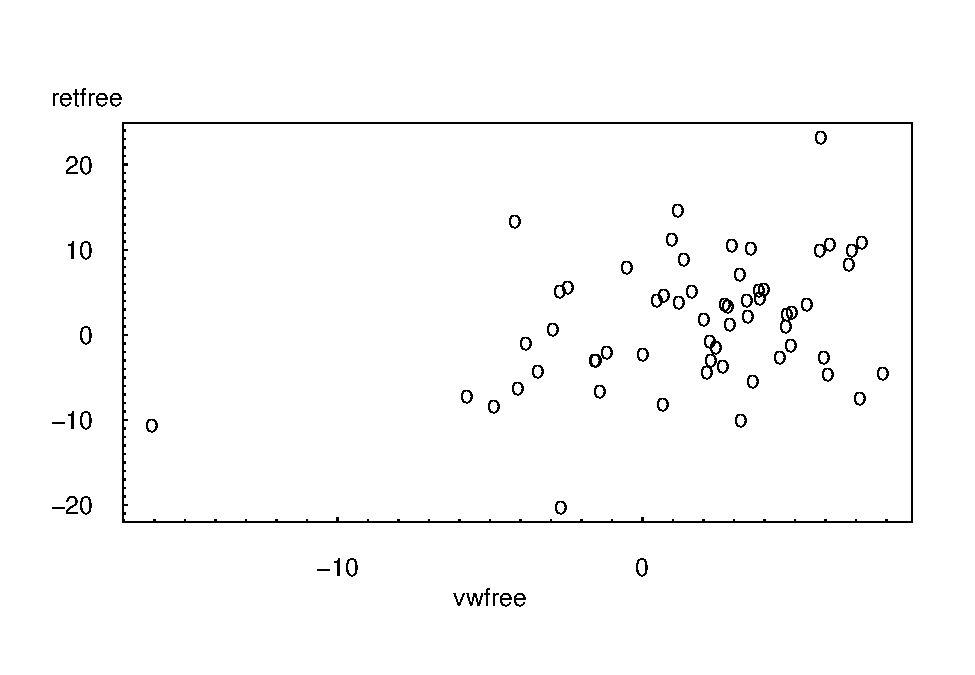
\includegraphics{LongPanelDataScripts_files/figure-latex/unnamed-chunk-70-1.pdf}

\hypertarget{plot-of-retfree-vs.-vwfree-for-90-insurance-firms}{%
\subsection{Plot of RETFREE vs.~VWFREE for 90 insurance firms}\label{plot-of-retfree-vs.-vwfree-for-90-insurance-firms}}

\begin{Shaded}
\begin{Highlighting}[]
\KeywordTok{plot}\NormalTok{(retfree }\OperatorTok{~}\StringTok{ }\NormalTok{vwfree, }\DataTypeTok{data =}\NormalTok{insbeta, }\DataTypeTok{type=}\StringTok{"p"}\NormalTok{, }\DataTypeTok{xaxt=}\StringTok{"n"}\NormalTok{, }\DataTypeTok{yaxt=}\StringTok{"n"}\NormalTok{, }\DataTypeTok{ylab=}\StringTok{""}\NormalTok{, }\DataTypeTok{xlab=}\StringTok{""}\NormalTok{, }\DataTypeTok{font=}\DecValTok{10}\NormalTok{, }\DataTypeTok{cex=}\DecValTok{1}\NormalTok{, }\DataTypeTok{pch=}\StringTok{"o"}\NormalTok{, }\DataTypeTok{las=}\DecValTok{1}\NormalTok{, }\DataTypeTok{mkh=}\FloatTok{0.0001}\NormalTok{, }\DataTypeTok{lwd=}\FloatTok{0.5}\NormalTok{)}
\KeywordTok{axis}\NormalTok{(}\DecValTok{2}\NormalTok{, }\DataTypeTok{at=}\KeywordTok{seq}\NormalTok{(}\OperatorTok{-}\DecValTok{70}\NormalTok{, }\DecValTok{110}\NormalTok{, }\DataTypeTok{by=}\DecValTok{10}\NormalTok{), }\DataTypeTok{las=}\DecValTok{1}\NormalTok{, }\DataTypeTok{font=}\DecValTok{10}\NormalTok{, }\DataTypeTok{cex=}\FloatTok{0.005}\NormalTok{, }\DataTypeTok{tck=}\FloatTok{0.01}\NormalTok{)}
\KeywordTok{axis}\NormalTok{(}\DecValTok{2}\NormalTok{, }\DataTypeTok{at=}\KeywordTok{seq}\NormalTok{(}\OperatorTok{-}\DecValTok{70}\NormalTok{, }\DecValTok{110}\NormalTok{, }\DataTypeTok{by=}\DecValTok{1}\NormalTok{), }\DataTypeTok{lab=}\NormalTok{F, }\DataTypeTok{tck=}\FloatTok{0.005}\NormalTok{)}
\KeywordTok{axis}\NormalTok{(}\DecValTok{1}\NormalTok{, }\DataTypeTok{at=}\KeywordTok{seq}\NormalTok{(}\OperatorTok{-}\DecValTok{20}\NormalTok{,}\DecValTok{10}\NormalTok{, }\DataTypeTok{by=}\DecValTok{10}\NormalTok{), }\DataTypeTok{font=}\DecValTok{10}\NormalTok{, }\DataTypeTok{cex=}\FloatTok{0.005}\NormalTok{, }\DataTypeTok{tck=}\FloatTok{0.01}\NormalTok{)}
\KeywordTok{axis}\NormalTok{(}\DecValTok{1}\NormalTok{, }\DataTypeTok{at=}\KeywordTok{seq}\NormalTok{(}\OperatorTok{-}\DecValTok{20}\NormalTok{,}\DecValTok{10}\NormalTok{, }\DataTypeTok{by=}\DecValTok{1}\NormalTok{), }\DataTypeTok{lab=}\NormalTok{F, }\DataTypeTok{tck=}\FloatTok{0.005}\NormalTok{)}
\KeywordTok{mtext}\NormalTok{(}\StringTok{"retfree"}\NormalTok{, }\DataTypeTok{side=}\DecValTok{2}\NormalTok{, }\DataTypeTok{line=}\DecValTok{0}\NormalTok{, }\DataTypeTok{at=}\DecValTok{115}\NormalTok{, }\DataTypeTok{font=}\DecValTok{10}\NormalTok{, }\DataTypeTok{cex=}\DecValTok{1}\NormalTok{, }\DataTypeTok{las=}\DecValTok{1}\NormalTok{)}
\KeywordTok{mtext}\NormalTok{(}\StringTok{"vwfree"}\NormalTok{, }\DataTypeTok{side=}\DecValTok{1}\NormalTok{, }\DataTypeTok{line=}\DecValTok{2}\NormalTok{, }\DataTypeTok{at=}\OperatorTok{-}\DecValTok{5}\NormalTok{, }\DataTypeTok{font=}\DecValTok{10}\NormalTok{, }\DataTypeTok{cex=}\DecValTok{1}\NormalTok{)}
\KeywordTok{mtext}\NormalTok{(}\StringTok{"RETFREE vs. VWFREE for 90 Insurance Firms"}\NormalTok{, }\DataTypeTok{side=}\DecValTok{1}\NormalTok{, }\DataTypeTok{line=}\DecValTok{4}\NormalTok{, }\DataTypeTok{at=}\OperatorTok{-}\DecValTok{5}\NormalTok{, }\DataTypeTok{font=}\DecValTok{10}\NormalTok{, }\DataTypeTok{cex=}\DecValTok{1}\NormalTok{)}
\end{Highlighting}
\end{Shaded}

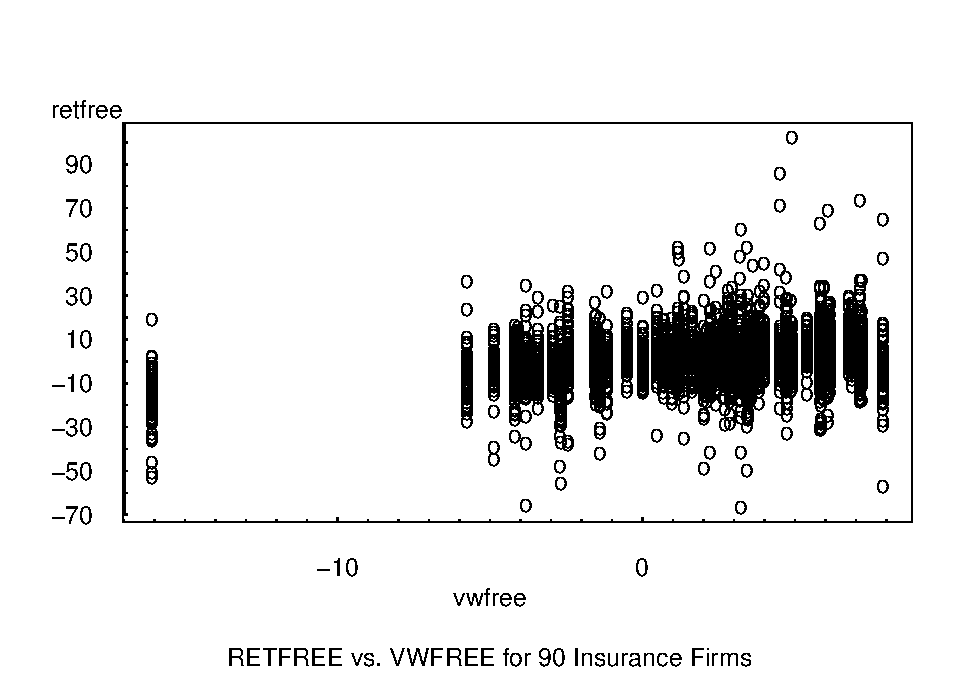
\includegraphics{LongPanelDataScripts_files/figure-latex/unnamed-chunk-71-1.pdf}

\hypertarget{plot-of-retfree-vs.-year-for-lincoln-insurance-company}{%
\subsection{Plot of RETFREE vs.~YEAR for Lincoln insurance company}\label{plot-of-retfree-vs.-year-for-lincoln-insurance-company}}

\begin{Shaded}
\begin{Highlighting}[]
\KeywordTok{plot}\NormalTok{(retfree }\OperatorTok{~}\StringTok{ }\NormalTok{YEAR, }\DataTypeTok{data =} \KeywordTok{subset}\NormalTok{(insbeta, insbeta}\OperatorTok{$}\NormalTok{PERMNO}\OperatorTok{==}\DecValTok{49015}\NormalTok{), }\DataTypeTok{type=}\StringTok{"o"}\NormalTok{, }\DataTypeTok{xaxt=}\StringTok{"n"}\NormalTok{, }\DataTypeTok{yaxt=}\StringTok{"n"}\NormalTok{, }\DataTypeTok{ylab=}\StringTok{""}\NormalTok{, }\DataTypeTok{xlab=}\StringTok{""}\NormalTok{, }\DataTypeTok{font=}\DecValTok{10}\NormalTok{, }\DataTypeTok{cex=}\DecValTok{1}\NormalTok{, }\DataTypeTok{pch=}\DecValTok{16}\NormalTok{, }\DataTypeTok{las=}\DecValTok{1}\NormalTok{, }\DataTypeTok{mkh=}\FloatTok{0.0001}\NormalTok{, }\DataTypeTok{lwd=}\FloatTok{0.5}\NormalTok{)}
\KeywordTok{axis}\NormalTok{(}\DecValTok{2}\NormalTok{, }\DataTypeTok{at=}\KeywordTok{seq}\NormalTok{(}\OperatorTok{-}\DecValTok{30}\NormalTok{, }\DecValTok{30}\NormalTok{, }\DataTypeTok{by=}\DecValTok{10}\NormalTok{), }\DataTypeTok{las=}\DecValTok{1}\NormalTok{, }\DataTypeTok{font=}\DecValTok{10}\NormalTok{, }\DataTypeTok{cex=}\FloatTok{0.005}\NormalTok{, }\DataTypeTok{tck=}\FloatTok{0.01}\NormalTok{)}
\KeywordTok{axis}\NormalTok{(}\DecValTok{2}\NormalTok{, }\DataTypeTok{at=}\KeywordTok{seq}\NormalTok{(}\OperatorTok{-}\DecValTok{30}\NormalTok{, }\DecValTok{30}\NormalTok{, }\DataTypeTok{by=}\DecValTok{1}\NormalTok{), }\DataTypeTok{lab=}\NormalTok{F, }\DataTypeTok{tck=}\FloatTok{0.005}\NormalTok{)}
\KeywordTok{axis}\NormalTok{(}\DecValTok{1}\NormalTok{, }\DataTypeTok{at=}\KeywordTok{seq}\NormalTok{(}\DecValTok{1995}\NormalTok{,}\DecValTok{2000}\NormalTok{, }\DataTypeTok{by=}\DecValTok{1}\NormalTok{), }\DataTypeTok{font=}\DecValTok{10}\NormalTok{, }\DataTypeTok{cex=}\FloatTok{0.005}\NormalTok{, }\DataTypeTok{tck=}\FloatTok{0.01}\NormalTok{)}
\KeywordTok{axis}\NormalTok{(}\DecValTok{1}\NormalTok{, }\DataTypeTok{at=}\KeywordTok{seq}\NormalTok{(}\DecValTok{1995}\NormalTok{,}\DecValTok{2000}\NormalTok{, }\DataTypeTok{by=}\FloatTok{0.1}\NormalTok{), }\DataTypeTok{lab=}\NormalTok{F, }\DataTypeTok{tck=}\FloatTok{0.005}\NormalTok{)}
\KeywordTok{mtext}\NormalTok{(}\StringTok{"retfree"}\NormalTok{, }\DataTypeTok{side=}\DecValTok{2}\NormalTok{, }\DataTypeTok{line=}\DecValTok{0}\NormalTok{, }\DataTypeTok{at=}\DecValTok{28}\NormalTok{, }\DataTypeTok{font=}\DecValTok{10}\NormalTok{, }\DataTypeTok{cex=}\DecValTok{1}\NormalTok{, }\DataTypeTok{las=}\DecValTok{1}\NormalTok{)}
\KeywordTok{mtext}\NormalTok{(}\StringTok{"year"}\NormalTok{, }\DataTypeTok{side=}\DecValTok{1}\NormalTok{, }\DataTypeTok{line=}\DecValTok{2}\NormalTok{, }\DataTypeTok{at=}\FloatTok{1997.50}\NormalTok{, }\DataTypeTok{font=}\DecValTok{10}\NormalTok{, }\DataTypeTok{cex=}\DecValTok{1}\NormalTok{)}
\KeywordTok{mtext}\NormalTok{(}\StringTok{"Lincoln RETFREE vs. YEAR"}\NormalTok{, }\DataTypeTok{side=}\DecValTok{1}\NormalTok{, }\DataTypeTok{line=}\DecValTok{5}\NormalTok{, }\DataTypeTok{at=}\FloatTok{1997.50}\NormalTok{, }\DataTypeTok{font=}\DecValTok{10}\NormalTok{, }\DataTypeTok{cex=}\DecValTok{1}\NormalTok{)}
\end{Highlighting}
\end{Shaded}

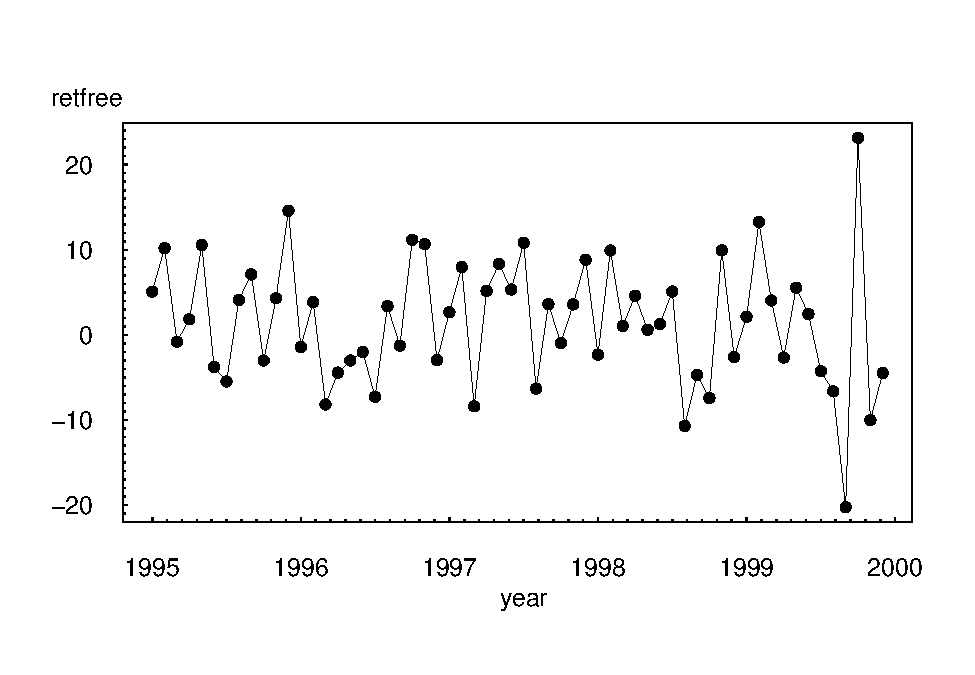
\includegraphics{LongPanelDataScripts_files/figure-latex/unnamed-chunk-72-1.pdf}

\hypertarget{table-8.2-summary-statistics-for-market-index-and-risk-free-security}{%
\subsection{Table 8.2 Summary statistics for market index and risk-free security}\label{table-8.2-summary-statistics-for-market-index-and-risk-free-security}}

\begin{Shaded}
\begin{Highlighting}[]
\NormalTok{LINCOLN<-}\KeywordTok{subset}\NormalTok{(insbeta, insbeta}\OperatorTok{$}\NormalTok{PERMNO}\OperatorTok{==}\DecValTok{49015}\NormalTok{)}
\KeywordTok{summary}\NormalTok{(LINCOLN[, }\KeywordTok{c}\NormalTok{(}\StringTok{"VWRETD"}\NormalTok{, }\StringTok{"SPRTRN"}\NormalTok{, }\StringTok{"riskf"}\NormalTok{, }\StringTok{"vwfree"}\NormalTok{, }\StringTok{"spfree"}\NormalTok{)])}
\end{Highlighting}
\end{Shaded}

\begin{verbatim}
     VWRETD             SPRTRN             riskf            vwfree        
 Min.   :-15.6765   Min.   :-14.5797   Min.   :0.2964   Min.   :-16.0683  
 1st Qu.: -0.2581   1st Qu.:  0.1612   1st Qu.:0.3811   1st Qu.: -0.6755  
 Median :  2.9464   Median :  2.6730   Median :0.4147   Median :  2.5174  
 Mean   :  2.0914   Mean   :  2.0380   Mean   :0.4075   Mean   :  1.6839  
 3rd Qu.:  4.9429   3rd Qu.:  5.0748   3rd Qu.:0.4267   3rd Qu.:  4.5654  
 Max.   :  8.3054   Max.   :  8.0294   Max.   :0.4829   Max.   :  7.8798  
     spfree        
 Min.   :-14.9714  
 1st Qu.: -0.2533  
 Median :  2.2244  
 Mean   :  1.6305  
 3rd Qu.:  4.6481  
 Max.   :  7.7330  
\end{verbatim}

\begin{Shaded}
\begin{Highlighting}[]
\NormalTok{sd1<-}\KeywordTok{sqrt}\NormalTok{(}\KeywordTok{diag}\NormalTok{(}\KeywordTok{var}\NormalTok{(insbeta[,}\KeywordTok{c}\NormalTok{(}\StringTok{"VWRETD"}\NormalTok{, }\StringTok{"SPRTRN"}\NormalTok{, }\StringTok{"riskf"}\NormalTok{, }\StringTok{"vwfree"}\NormalTok{, }\StringTok{"spfree"}\NormalTok{)])))}
\NormalTok{sd1}
\end{Highlighting}
\end{Shaded}

\begin{verbatim}
    VWRETD     SPRTRN      riskf     vwfree     spfree 
4.09890088 3.98794716 0.03380599 4.09997511 3.98932881 
\end{verbatim}

\begin{Shaded}
\begin{Highlighting}[]
\KeywordTok{cor}\NormalTok{(LINCOLN[,}\KeywordTok{c}\NormalTok{(}\StringTok{"VWRETD"}\NormalTok{, }\StringTok{"SPRTRN"}\NormalTok{, }\StringTok{"riskf"}\NormalTok{, }\StringTok{"vwfree"}\NormalTok{, }\StringTok{"spfree"}\NormalTok{)])}
\end{Highlighting}
\end{Shaded}

\begin{verbatim}
           VWRETD      SPRTRN       riskf      vwfree      spfree
VWRETD  1.0000000  0.97950897 -0.02765660  0.99996603  0.97940410
SPRTRN  0.9795090  1.00000000 -0.03663843  0.97955443  0.99996414
riskf  -0.0276566 -0.03663843  1.00000000 -0.03589477 -0.04509984
vwfree  0.9999660  0.97955443 -0.03589477  1.00000000  0.97951935
spfree  0.9794041  0.99996414 -0.04509984  0.97951935  1.00000000
\end{verbatim}

Table 8.2 summarizes the performance of the market through the return from the value-weighted index, \texttt{VWRETD}, and risk free instrument, \texttt{RISKFREE}. We also consider the difference between the two, \texttt{VWFREE}, and interpret this to be the return from the market in excess of the risk-free rate.

\hypertarget{table-8.3-summary-statistics-for-individual-security-returns}{%
\subsection{TABLE 8.3 Summary statistics for individual security returns}\label{table-8.3-summary-statistics-for-individual-security-returns}}

\begin{Shaded}
\begin{Highlighting}[]
\KeywordTok{summary}\NormalTok{(insbeta[,}\KeywordTok{c}\NormalTok{(}\StringTok{"RET"}\NormalTok{, }\StringTok{"retfree"}\NormalTok{, }\StringTok{"PRC"}\NormalTok{)]) }
\end{Highlighting}
\end{Shaded}

\begin{verbatim}
      RET              retfree              PRC          
 Min.   :-66.1972   Min.   :-66.5785   Min.   :    0.81  
 1st Qu.: -3.8462   1st Qu.: -4.2428   1st Qu.:   14.25  
 Median :  0.7453   Median :  0.3402   Median :   26.88  
 Mean   :  1.0521   Mean   :  0.6446   Mean   :  547.11  
 3rd Qu.:  5.8823   3rd Qu.:  5.4675   3rd Qu.:   45.89  
 Max.   :102.5000   Max.   :102.0850   Max.   :78305.00  
\end{verbatim}

\begin{Shaded}
\begin{Highlighting}[]
\CommentTok{# STANDARD DEVIATION}
\NormalTok{sd1<-}\KeywordTok{sqrt}\NormalTok{(}\KeywordTok{diag}\NormalTok{(}\KeywordTok{var}\NormalTok{(insbeta[,}\KeywordTok{c}\NormalTok{(}\StringTok{"RET"}\NormalTok{, }\StringTok{"retfree"}\NormalTok{, }\StringTok{"PRC"}\NormalTok{)])))}
\NormalTok{sd1}
\end{Highlighting}
\end{Shaded}

\begin{verbatim}
       RET    retfree        PRC 
  10.03772   10.03552 5178.49653 
\end{verbatim}

\begin{Shaded}
\begin{Highlighting}[]
\KeywordTok{cor}\NormalTok{(insbeta[,}\KeywordTok{c}\NormalTok{(}\StringTok{"RET"}\NormalTok{, }\StringTok{"VWRETD"}\NormalTok{, }\StringTok{"SPRTRN"}\NormalTok{, }\StringTok{"riskf"}\NormalTok{, }\StringTok{"retfree"}\NormalTok{, }\StringTok{"vwfree"}\NormalTok{, }\StringTok{"spfree"}\NormalTok{)])}
\end{Highlighting}
\end{Shaded}

\begin{verbatim}
               RET     VWRETD      SPRTRN       riskf    retfree
RET     1.00000000  0.2937725  0.28237030  0.06693926 0.99999435
VWRETD  0.29377254  1.0000000  0.97950897 -0.02765660 0.29393029
SPRTRN  0.28237030  0.9795090  1.00000000 -0.03663843 0.28255580
riskf   0.06693926 -0.0276566 -0.03663843  1.00000000 0.06358534
retfree 0.99999435  0.2939303  0.28255580  0.06358534 1.00000000
vwfree  0.29314362  0.9999660  0.97955443 -0.03589477 0.29332899
spfree  0.28170525  0.9794041  0.99996414 -0.04509984 0.28191911
             vwfree      spfree
RET      0.29314362  0.28170525
VWRETD   0.99996603  0.97940410
SPRTRN   0.97955443  0.99996414
riskf   -0.03589477 -0.04509984
retfree  0.29332899  0.28191911
vwfree   1.00000000  0.97951935
spfree   0.97951935  1.00000000
\end{verbatim}

Table 8.3 summarizes the performance of individual securities through the monthly return, \texttt{RET}. These summary statistics are based on 5,400 monthly observations taken from 90 firms. The difference between the return and the corresponding risk-free instrument is \texttt{RETFREE}.

\hypertarget{table-8.4-fixed-effects-models}{%
\subsection{TABLE 8.4 Fixed effects models}\label{table-8.4-fixed-effects-models}}

\begin{Shaded}
\begin{Highlighting}[]
\CommentTok{#HOMOGENEOUS MODEL}
\NormalTok{insbetahomo<-}\KeywordTok{gls}\NormalTok{(retfree}\OperatorTok{~}\NormalTok{vwfree, }\DataTypeTok{method=}\StringTok{"REML"}\NormalTok{, }\DataTypeTok{data=}\NormalTok{insbeta) }
\KeywordTok{anova}\NormalTok{(insbetahomo)}
\end{Highlighting}
\end{Shaded}

\begin{verbatim}
Denom. DF: 5398 
            numDF  F-value p-value
(Intercept)     1  24.3686  <.0001
vwfree          1 508.1788  <.0001
\end{verbatim}

\begin{Shaded}
\begin{Highlighting}[]
\NormalTok{insbetahomo}\OperatorTok{$}\NormalTok{sigma}\OperatorTok{^}\DecValTok{2}
\end{Highlighting}
\end{Shaded}

\begin{verbatim}
[1] 92.06322
\end{verbatim}

\begin{Shaded}
\begin{Highlighting}[]
\KeywordTok{AIC}\NormalTok{(insbetahomo)}
\end{Highlighting}
\end{Shaded}

\begin{verbatim}
[1] 39757.19
\end{verbatim}

\begin{Shaded}
\begin{Highlighting}[]
\KeywordTok{logLik}\NormalTok{(insbetahomo)}\OperatorTok{*}\NormalTok{(}\OperatorTok{-}\DecValTok{2}\NormalTok{)}
\end{Highlighting}
\end{Shaded}

\begin{verbatim}
'log Lik.' 39751.19 (df=3)
\end{verbatim}

\begin{Shaded}
\begin{Highlighting}[]
\NormalTok{insbeta}\OperatorTok{$}\NormalTok{FACPERM<-}\KeywordTok{factor}\NormalTok{(insbeta}\OperatorTok{$}\NormalTok{PERMNO)}
\CommentTok{#VARIABLE INTERCEPT MODEL}
\NormalTok{insbetafx1<-}\KeywordTok{gls}\NormalTok{(retfree}\OperatorTok{~}\NormalTok{vwfree}\OperatorTok{+}\NormalTok{FACPERM, }\DataTypeTok{method=}\StringTok{"REML"}\NormalTok{, }\DataTypeTok{data=}\NormalTok{insbeta)}
\KeywordTok{anova}\NormalTok{(insbetafx1)}
\end{Highlighting}
\end{Shaded}

\begin{verbatim}
Denom. DF: 5309 
            numDF  F-value p-value
(Intercept)     1  24.2193  <.0001
vwfree          1 505.0665  <.0001
FACPERM        89   0.6285  0.9975
\end{verbatim}

\begin{Shaded}
\begin{Highlighting}[]
\NormalTok{insbetafx1}\OperatorTok{$}\NormalTok{sigma}\OperatorTok{^}\DecValTok{2}
\end{Highlighting}
\end{Shaded}

\begin{verbatim}
[1] 92.63053
\end{verbatim}

\begin{Shaded}
\begin{Highlighting}[]
\KeywordTok{AIC}\NormalTok{(insbetafx1)}
\end{Highlighting}
\end{Shaded}

\begin{verbatim}
[1] 39672.63
\end{verbatim}

\begin{Shaded}
\begin{Highlighting}[]
\KeywordTok{logLik}\NormalTok{(insbetafx1)}\OperatorTok{*}\NormalTok{(}\OperatorTok{-}\DecValTok{2}\NormalTok{)}
\end{Highlighting}
\end{Shaded}

\begin{verbatim}
'log Lik.' 39488.63 (df=92)
\end{verbatim}

\begin{Shaded}
\begin{Highlighting}[]
\CommentTok{#VARIALBE SLOPES MODEL}
\NormalTok{insbetafx2<-}\KeywordTok{gls}\NormalTok{(retfree}\OperatorTok{~}\NormalTok{vwfree}\OperatorTok{*}\NormalTok{FACPERM}\OperatorTok{-}\NormalTok{vwfree}\OperatorTok{-}\NormalTok{FACPERM, }\DataTypeTok{method=}\StringTok{"REML"}\NormalTok{, }\DataTypeTok{data=}\NormalTok{insbeta)}
\KeywordTok{anova}\NormalTok{(insbetafx2)}
\end{Highlighting}
\end{Shaded}

\begin{verbatim}
Denom. DF: 5309 
               numDF   F-value p-value
(Intercept)        1 24.712995  <.0001
vwfree:FACPERM    90  7.562791  <.0001
\end{verbatim}

\begin{Shaded}
\begin{Highlighting}[]
\NormalTok{insbetafx2}\OperatorTok{$}\NormalTok{sigma}\OperatorTok{^}\DecValTok{2}
\end{Highlighting}
\end{Shaded}

\begin{verbatim}
[1] 90.78022
\end{verbatim}

\begin{Shaded}
\begin{Highlighting}[]
\KeywordTok{AIC}\NormalTok{(insbetafx2)}
\end{Highlighting}
\end{Shaded}

\begin{verbatim}
[1] 39830.52
\end{verbatim}

\begin{Shaded}
\begin{Highlighting}[]
\KeywordTok{logLik}\NormalTok{(insbetafx2)}\OperatorTok{*}\NormalTok{(}\OperatorTok{-}\DecValTok{2}\NormalTok{)}
\end{Highlighting}
\end{Shaded}

\begin{verbatim}
'log Lik.' 39646.52 (df=92)
\end{verbatim}

\begin{Shaded}
\begin{Highlighting}[]
\CommentTok{#VARIABLE INTERCEPTS AND SLOPES MODEL}
\NormalTok{insbetafx3<-}\KeywordTok{gls}\NormalTok{(retfree}\OperatorTok{~}\NormalTok{vwfree}\OperatorTok{*}\NormalTok{FACPERM, }\DataTypeTok{method=}\StringTok{"REML"}\NormalTok{, }\DataTypeTok{data=}\NormalTok{insbeta)}
\KeywordTok{anova}\NormalTok{(insbetafx3)}
\end{Highlighting}
\end{Shaded}

\begin{verbatim}
Denom. DF: 5220 
               numDF  F-value p-value
(Intercept)        1  24.6569  <.0001
vwfree             1 514.1906  <.0001
FACPERM           89   0.6399  0.9966
vwfree:FACPERM    89   2.0776  <.0001
\end{verbatim}

\begin{Shaded}
\begin{Highlighting}[]
\NormalTok{insbetafx3}\OperatorTok{$}\NormalTok{sigma}\OperatorTok{^}\DecValTok{2}
\end{Highlighting}
\end{Shaded}

\begin{verbatim}
[1] 90.98683
\end{verbatim}

\begin{Shaded}
\begin{Highlighting}[]
\KeywordTok{AIC}\NormalTok{(insbetafx3)}
\end{Highlighting}
\end{Shaded}

\begin{verbatim}
[1] 39712.59
\end{verbatim}

\begin{Shaded}
\begin{Highlighting}[]
\KeywordTok{logLik}\NormalTok{(insbetafx3)}\OperatorTok{*}\NormalTok{(}\OperatorTok{-}\DecValTok{2}\NormalTok{)}
\end{Highlighting}
\end{Shaded}

\begin{verbatim}
'log Lik.' 39350.59 (df=181)
\end{verbatim}

\begin{Shaded}
\begin{Highlighting}[]
\CommentTok{#VARIABLE SLOPES MODEL WITH AR(1) TERM}
\NormalTok{insbetafx4<-}\KeywordTok{gls}\NormalTok{(retfree}\OperatorTok{~}\NormalTok{vwfree}\OperatorTok{:}\NormalTok{FACPERM, }\DataTypeTok{data=}\NormalTok{insbeta, }\DataTypeTok{method=}\StringTok{"REML"}\NormalTok{, }\DataTypeTok{correlation=}\KeywordTok{corAR1}\NormalTok{(}\DataTypeTok{form=}\OperatorTok{~}\DecValTok{1}\OperatorTok{|}\NormalTok{PERMNO)) }\CommentTok{#Model probably not working}
\KeywordTok{anova}\NormalTok{(insbetafx4)}
\end{Highlighting}
\end{Shaded}

\begin{verbatim}
Denom. DF: 5309 
               numDF   F-value p-value
(Intercept)        1 29.285237  <.0001
vwfree:FACPERM    90  7.941803  <.0001
\end{verbatim}

\begin{Shaded}
\begin{Highlighting}[]
\NormalTok{insbetafx4}\OperatorTok{$}\NormalTok{sigma}\OperatorTok{^}\DecValTok{2}
\end{Highlighting}
\end{Shaded}

\begin{verbatim}
[1] 90.76872
\end{verbatim}

\begin{Shaded}
\begin{Highlighting}[]
\KeywordTok{AIC}\NormalTok{(insbetafx4)}
\end{Highlighting}
\end{Shaded}

\begin{verbatim}
[1] 39796.92
\end{verbatim}

\begin{Shaded}
\begin{Highlighting}[]
\KeywordTok{logLik}\NormalTok{(insbetafx4)}\OperatorTok{*}\NormalTok{(}\OperatorTok{-}\DecValTok{2}\NormalTok{)}
\end{Highlighting}
\end{Shaded}

\begin{verbatim}
'log Lik.' 39610.92 (df=93)
\end{verbatim}

\begin{Shaded}
\begin{Highlighting}[]
\NormalTok{insbetafx4}\OperatorTok{$}\NormalTok{modelStruct}
\end{Highlighting}
\end{Shaded}

\begin{verbatim}
corStruct  parameters:
[1] -0.1689266
\end{verbatim}

Table 8.4 summarizes the fit of each model. Based on these fits, we will use the variable slopes with an \(AR(1)\) error term model as the baseline for investigating time-varying coefficients.

Then we can include random effects:

\begin{Shaded}
\begin{Highlighting}[]
\NormalTok{insbetarm<-}\KeywordTok{lme}\NormalTok{(retfree}\OperatorTok{~}\NormalTok{vwfree, }\DataTypeTok{data=}\NormalTok{insbeta, }\DataTypeTok{random=}\OperatorTok{~}\NormalTok{vwfree}\DecValTok{-1}\OperatorTok{|}\NormalTok{PERMNO) }\CommentTok{#Random - Effects Model}

\NormalTok{insbetarco<-}\KeywordTok{lme}\NormalTok{(retfree}\OperatorTok{~}\NormalTok{vwfree, }\DataTypeTok{data=}\NormalTok{insbeta, }\DataTypeTok{random=}\OperatorTok{~}\DecValTok{1}\OperatorTok{+}\NormalTok{vwfree}\OperatorTok{|}\NormalTok{PERMNO, }\DataTypeTok{correlation=}\KeywordTok{corAR1}\NormalTok{(}\DataTypeTok{form=}\OperatorTok{~}\DecValTok{1}\OperatorTok{|}\NormalTok{PERMNO),}\DataTypeTok{control =} \KeywordTok{lmeControl}\NormalTok{(}\DataTypeTok{opt =} \StringTok{"optim"}\NormalTok{))}

\CommentTok{#due to convergence problem, I add the "control = lmeControl(opt = "optim")".}

\CommentTok{#Random - Coefficients Model}
\KeywordTok{summary}\NormalTok{(insbetarm)}
\end{Highlighting}
\end{Shaded}

\begin{verbatim}
Linear mixed-effects model fit by REML
 Data: insbeta 
       AIC      BIC    logLik
  39738.53 39764.91 -19865.27

Random effects:
 Formula: ~vwfree - 1 | PERMNO
           vwfree Residual
StdDev: 0.2569603 9.527865

Fixed effects: retfree ~ vwfree 
                 Value  Std.Error   DF   t-value p-value
(Intercept) -0.5644229 0.14016877 5309 -4.026737   1e-04
vwfree       0.7179819 0.04164033 5309 17.242464   0e+00
 Correlation: 
       (Intr)
vwfree -0.289

Standardized Within-Group Residuals:
        Min          Q1         Med          Q3         Max 
-7.18150077 -0.49947031 -0.02643177  0.46193572 10.17362517 

Number of Observations: 5400
Number of Groups: 90 
\end{verbatim}

\begin{Shaded}
\begin{Highlighting}[]
\KeywordTok{summary}\NormalTok{(insbetarco)}
\end{Highlighting}
\end{Shaded}

\begin{verbatim}
Linear mixed-effects model fit by REML
 Data: insbeta 
      AIC      BIC   logLik
  39697.8 39743.95 -19841.9

Random effects:
 Formula: ~1 + vwfree | PERMNO
 Structure: General positive-definite, Log-Cholesky parametrization
            StdDev    Corr  
(Intercept) 0.5759112 (Intr)
vwfree      0.3182517 -0.831
Residual    9.5058076       

Correlation Structure: AR(1)
 Formula: ~1 | PERMNO 
 Parameter estimate(s):
        Phi 
-0.08830483 
Fixed effects: retfree ~ vwfree 
                 Value  Std.Error   DF   t-value p-value
(Intercept) -0.5905640 0.14322023 5309 -4.123468       0
vwfree       0.7378101 0.04596025 5309 16.053222       0
 Correlation: 
       (Intr)
vwfree -0.508

Standardized Within-Group Residuals:
        Min          Q1         Med          Q3         Max 
-7.20057083 -0.49733487 -0.02677384  0.46069650 10.22355808 

Number of Observations: 5400
Number of Groups: 90 
\end{verbatim}

Cleaning up companies with more than one Ticker names but having the same \texttt{PERMNO}:

\begin{Shaded}
\begin{Highlighting}[]
\NormalTok{tab<-}\KeywordTok{as.matrix}\NormalTok{(}\KeywordTok{xtabs}\NormalTok{(}\OperatorTok{~}\NormalTok{PERMNO}\OperatorTok{+}\NormalTok{TICKER, insbeta)) }\CommentTok{#a logical matrix cross-tabulation of PERMNO and TIcker}
\KeywordTok{which}\NormalTok{(}\KeywordTok{rowSums}\NormalTok{(tab}\OperatorTok{>}\DecValTok{0}\NormalTok{)}\OperatorTok{>}\DecValTok{1}\NormalTok{)}
\end{Highlighting}
\end{Shaded}

\begin{verbatim}
10085 10388 10933 11203 11371 11406 11713 22198 37226 48901 52936 58393 
    1     5    10    12    13    14    16    24    30    41    44    50 
60687 76099 76697 77052 77815 
   56    72    79    83    86 
\end{verbatim}

\begin{Shaded}
\begin{Highlighting}[]
\CommentTok{# PERMNOs that have more than one ticker}
\CommentTok{#10085 10388 10933 11203 11371 11406 11713 22198 37226 48901 52936 58393 60687 }
\CommentTok{#    1     5    10    12    13    14    16    24    30    41    44    50    56 }
\CommentTok{#76099 76697 77052 77815 }
\CommentTok{#   72    79    83    86 }
\CommentTok{# For each PERMNO go through the following code check on the the TICKER names and frequency}
\CommentTok{# which(tab["10388",]>0)}
\CommentTok{#TREN  TWK }
\CommentTok{#  96   99 }
\CommentTok{#> tab["10388", c(96,99)]}
\CommentTok{# TREN  TWK }
\CommentTok{#  57    3  # THIS SHOWS THE FREQUENCY AS WELL AS THE TICKER NAMES FOR ONE SINGLE PERMNO "10388"}
\end{Highlighting}
\end{Shaded}

Recode Tickers:

\begin{Shaded}
\begin{Highlighting}[]
\NormalTok{insbeta}\OperatorTok{$}\NormalTok{TICKER[insbeta}\OperatorTok{$}\NormalTok{PERMNO}\OperatorTok{==}\StringTok{"10085"}\NormalTok{]<-}\StringTok{"UICI"}
\NormalTok{insbeta}\OperatorTok{$}\NormalTok{TICKER[insbeta}\OperatorTok{$}\NormalTok{PERMNO}\OperatorTok{==}\StringTok{"10388"}\NormalTok{]<-}\StringTok{"TREN"}
\NormalTok{insbeta}\OperatorTok{$}\NormalTok{TICKER[insbeta}\OperatorTok{$}\NormalTok{PERMNO}\OperatorTok{==}\StringTok{"10933"}\NormalTok{]<-}\StringTok{"MKL"}
\NormalTok{insbeta}\OperatorTok{$}\NormalTok{TICKER[insbeta}\OperatorTok{$}\NormalTok{PERMNO}\OperatorTok{==}\StringTok{"11203"}\NormalTok{]<-}\StringTok{"PXT"}
\NormalTok{insbeta}\OperatorTok{$}\NormalTok{TICKER[insbeta}\OperatorTok{$}\NormalTok{PERMNO}\OperatorTok{==}\StringTok{"11371"}\NormalTok{]<-}\StringTok{"HCCC"}
\NormalTok{insbeta}\OperatorTok{$}\NormalTok{TICKER[insbeta}\OperatorTok{$}\NormalTok{PERMNO}\OperatorTok{==}\StringTok{"11406"}\NormalTok{]<-}\StringTok{"CSH"}
\NormalTok{insbeta}\OperatorTok{$}\NormalTok{TICKER[insbeta}\OperatorTok{$}\NormalTok{PERMNO}\OperatorTok{==}\StringTok{"11713"}\NormalTok{]<-}\StringTok{"PTAC"}
\NormalTok{insbeta}\OperatorTok{$}\NormalTok{TICKER[insbeta}\OperatorTok{$}\NormalTok{PERMNO}\OperatorTok{==}\StringTok{"22198"}\NormalTok{]<-}\StringTok{"CRLC"}
\NormalTok{insbeta}\OperatorTok{$}\NormalTok{TICKER[insbeta}\OperatorTok{$}\NormalTok{PERMNO}\OperatorTok{==}\StringTok{"37226"}\NormalTok{]<-}\StringTok{"FOM"}
\NormalTok{insbeta}\OperatorTok{$}\NormalTok{TICKER[insbeta}\OperatorTok{$}\NormalTok{PERMNO}\OperatorTok{==}\StringTok{"48901"}\NormalTok{]<-}\StringTok{"MLA"}
\NormalTok{insbeta}\OperatorTok{$}\NormalTok{TICKER[insbeta}\OperatorTok{$}\NormalTok{PERMNO}\OperatorTok{==}\StringTok{"52936"}\NormalTok{]<-}\StringTok{"MCY"}
\NormalTok{insbeta}\OperatorTok{$}\NormalTok{TICKER[insbeta}\OperatorTok{$}\NormalTok{PERMNO}\OperatorTok{==}\StringTok{"58393"}\NormalTok{]<-}\StringTok{"RLR"}
\NormalTok{insbeta}\OperatorTok{$}\NormalTok{TICKER[insbeta}\OperatorTok{$}\NormalTok{PERMNO}\OperatorTok{==}\StringTok{"60687"}\NormalTok{]<-}\StringTok{"AFG"}
\NormalTok{insbeta}\OperatorTok{$}\NormalTok{TICKER[insbeta}\OperatorTok{$}\NormalTok{PERMNO}\OperatorTok{==}\StringTok{"76099"}\NormalTok{]<-}\StringTok{"DFG"}
\NormalTok{insbeta}\OperatorTok{$}\NormalTok{TICKER[insbeta}\OperatorTok{$}\NormalTok{PERMNO}\OperatorTok{==}\StringTok{"76697"}\NormalTok{]<-}\StringTok{"FHS"}
\NormalTok{insbeta}\OperatorTok{$}\NormalTok{TICKER[insbeta}\OperatorTok{$}\NormalTok{PERMNO}\OperatorTok{==}\StringTok{"77052"}\NormalTok{]<-}\StringTok{"UWZ"}
\NormalTok{insbeta}\OperatorTok{$}\NormalTok{TICKER[insbeta}\OperatorTok{$}\NormalTok{PERMNO}\OperatorTok{==}\StringTok{"77815"}\NormalTok{]<-}\StringTok{"EQ"}
\end{Highlighting}
\end{Shaded}

Retuen the following checking the consistency between \texttt{PERMNO} and \texttt{TICKER}:

\begin{Shaded}
\begin{Highlighting}[]
\NormalTok{tab<-}\KeywordTok{as.matrix}\NormalTok{(}\KeywordTok{xtabs}\NormalTok{(}\OperatorTok{~}\NormalTok{PERMNO}\OperatorTok{+}\NormalTok{TICKER, insbeta)) }
\KeywordTok{which}\NormalTok{(}\KeywordTok{rowSums}\NormalTok{(tab}\OperatorTok{>}\DecValTok{0}\NormalTok{)}\OperatorTok{>}\DecValTok{1}\NormalTok{) }\CommentTok{#RESULT SHOULD BE ZERO}
\end{Highlighting}
\end{Shaded}

\begin{verbatim}
named integer(0)
\end{verbatim}

\hypertarget{figure-8.1-trellis-plot-of-returns-versus-market-return}{%
\subsection{Figure 8.1: Trellis plot of returns versus market return}\label{figure-8.1-trellis-plot-of-returns-versus-market-return}}

\begin{Shaded}
\begin{Highlighting}[]
\CommentTok{#PRODUCE A TRELLIS PLOT TO SHOW VARYING BETAS}
\KeywordTok{library}\NormalTok{(lattice)}
\NormalTok{insbeta}\OperatorTok{$}\NormalTok{ID=}\KeywordTok{factor}\NormalTok{(insbeta}\OperatorTok{$}\NormalTok{PERMNO)}
\NormalTok{insbeta}\OperatorTok{$}\NormalTok{TK=}\KeywordTok{factor}\NormalTok{(insbeta}\OperatorTok{$}\NormalTok{TICKER)}
\NormalTok{sampbeta <-}\StringTok{ }\KeywordTok{subset}\NormalTok{(insbeta, ID }\OperatorTok\StringTok{ }\KeywordTok{sample}\NormalTok{(}\KeywordTok{levels}\NormalTok{(insbeta}\OperatorTok{$}\NormalTok{ID), }\DecValTok{18}\NormalTok{, }\DataTypeTok{replace=}\OtherTok{FALSE}\NormalTok{) )}

\KeywordTok{xyplot}\NormalTok{(RET }\OperatorTok{~}\StringTok{ }\NormalTok{VWRETD }\OperatorTok{|}\StringTok{ }\NormalTok{TK, }\DataTypeTok{data=}\NormalTok{sampbeta, }\DataTypeTok{layout=}\KeywordTok{c}\NormalTok{(}\DecValTok{6}\NormalTok{,}\DecValTok{3}\NormalTok{,}\DecValTok{1}\NormalTok{), }\DataTypeTok{panel =} \ControlFlowTok{function}\NormalTok{(x, y) \{}
 \KeywordTok{panel.grid}\NormalTok{()}
 \KeywordTok{panel.xyplot}\NormalTok{(x, y)}
 \KeywordTok{panel.loess}\NormalTok{(x, y, }\DataTypeTok{span =} \FloatTok{1.5}\NormalTok{)}
\NormalTok{ \})}
\end{Highlighting}
\end{Shaded}

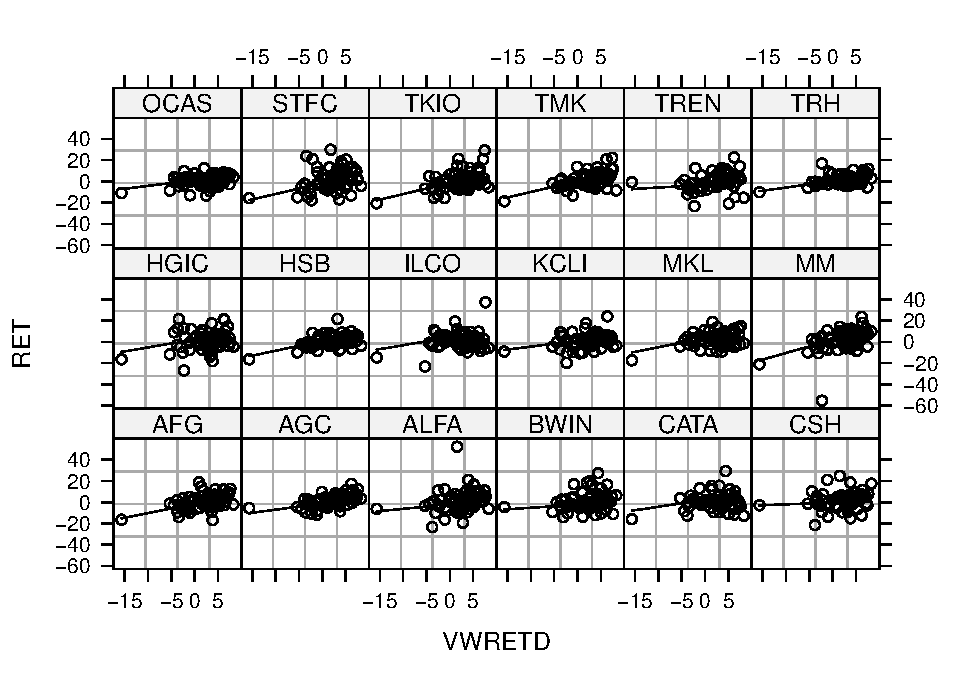
\includegraphics{LongPanelDataScripts_files/figure-latex/unnamed-chunk-80-1.pdf}

\hypertarget{binary-dependent-variables}{%
\chapter{Binary Dependent Variables}\label{binary-dependent-variables}}

\hypertarget{import-data-7}{%
\section{Import Data}\label{import-data-7}}

\begin{Shaded}
\begin{Highlighting}[]
\NormalTok{taxprep=}\KeywordTok{read.table}\NormalTok{(}\StringTok{"TXTData/TaxPrep.txt"}\NormalTok{, }\DataTypeTok{sep =}\StringTok{"}\CharTok{\textbackslash{}t}\StringTok{"}\NormalTok{, }\DataTypeTok{quote =} \StringTok{""}\NormalTok{,}\DataTypeTok{header=}\OtherTok{TRUE}\NormalTok{)}

\CommentTok{#taxprep=read.table(choose.files(), header=TRUE, sep="\textbackslash{}t")}
\end{Highlighting}
\end{Shaded}

Data for this study are from the Statistics of Income (SOI) Panel of Individual Returns, a part of the Ernst and Young/University of Michigan Tax Research Database. The SOI Panel represents a simple random sample of unaudited individual income tax returns filed for tax years 1979-1990. The data are compiled from a stratified probability sample of unaudited individual income tax returns, Forms 1040, 1040A and 1040EZ, filed by U.S. taxpayers. The estimates that are obtained from these data are intended to represent all returns filed for the income tax years under review. All returns processed are subjected to sampling except tentative and amended returns.

\begin{longtable}[]{@{}ll@{}}
\toprule
\begin{minipage}[b]{0.09\columnwidth}\raggedright
Variable\strut
\end{minipage} & \begin{minipage}[b]{0.86\columnwidth}\raggedright
Description\strut
\end{minipage}\tabularnewline
\midrule
\endhead
\begin{minipage}[t]{0.09\columnwidth}\raggedright
MS\strut
\end{minipage} & \begin{minipage}[t]{0.86\columnwidth}\raggedright
is an indicator variable of the taxpayer's marital status. It is coded one if the taxpayer is married and zero otherwise.\strut
\end{minipage}\tabularnewline
\begin{minipage}[t]{0.09\columnwidth}\raggedright
HH\strut
\end{minipage} & \begin{minipage}[t]{0.86\columnwidth}\raggedright
is an indicator variable, one if the taxpayer is a head of household and zero otherwise.\strut
\end{minipage}\tabularnewline
\begin{minipage}[t]{0.09\columnwidth}\raggedright
DEPEND\strut
\end{minipage} & \begin{minipage}[t]{0.86\columnwidth}\raggedright
is the number of dependents claimed by the taxpayer.\strut
\end{minipage}\tabularnewline
\begin{minipage}[t]{0.09\columnwidth}\raggedright
AGE\strut
\end{minipage} & \begin{minipage}[t]{0.86\columnwidth}\raggedright
is the presence of an indicator for age 65 or over.\strut
\end{minipage}\tabularnewline
\begin{minipage}[t]{0.09\columnwidth}\raggedright
F1040A\strut
\end{minipage} & \begin{minipage}[t]{0.86\columnwidth}\raggedright
is an indicator variable of the taxpayer's filing type. It is coded one if the taxpayer uses Form 1040A and zero otherwise.\strut
\end{minipage}\tabularnewline
\begin{minipage}[t]{0.09\columnwidth}\raggedright
F1040EZ\strut
\end{minipage} & \begin{minipage}[t]{0.86\columnwidth}\raggedright
is an indicator variable of the taxpayer's filing type. It is coded one if the taxpayer uses Form 1040EZ and zero otherwise.\strut
\end{minipage}\tabularnewline
\begin{minipage}[t]{0.09\columnwidth}\raggedright
TPI\strut
\end{minipage} & \begin{minipage}[t]{0.86\columnwidth}\raggedright
is the sum of all positive income line items on the return.\strut
\end{minipage}\tabularnewline
\begin{minipage}[t]{0.09\columnwidth}\raggedright
TXRT\strut
\end{minipage} & \begin{minipage}[t]{0.86\columnwidth}\raggedright
is a marginal tax rate. It is computed on TPI less exemptions and the standard deduction.\strut
\end{minipage}\tabularnewline
\begin{minipage}[t]{0.09\columnwidth}\raggedright
MR\strut
\end{minipage} & \begin{minipage}[t]{0.86\columnwidth}\raggedright
is an exogenous marginal tax rate. It is computed on TPI less exemptions and the standard deduction.\strut
\end{minipage}\tabularnewline
\begin{minipage}[t]{0.09\columnwidth}\raggedright
EMP\strut
\end{minipage} & \begin{minipage}[t]{0.86\columnwidth}\raggedright
is an indicator variable, one if Schedule C or F is present and zero otherwise. Self-employed taxpayers have greater need for professional assistance to reduce the reporting risks of doing business.\strut
\end{minipage}\tabularnewline
\begin{minipage}[t]{0.09\columnwidth}\raggedright
PREP\strut
\end{minipage} & \begin{minipage}[t]{0.86\columnwidth}\raggedright
is a variable indicating the presence of a paid preparer.\strut
\end{minipage}\tabularnewline
\begin{minipage}[t]{0.09\columnwidth}\raggedright
TAX\strut
\end{minipage} & \begin{minipage}[t]{0.86\columnwidth}\raggedright
is the tax liability on the return.\strut
\end{minipage}\tabularnewline
\begin{minipage}[t]{0.09\columnwidth}\raggedright
SUBJECT\strut
\end{minipage} & \begin{minipage}[t]{0.86\columnwidth}\raggedright
Subject identifier, 1-258.\strut
\end{minipage}\tabularnewline
\begin{minipage}[t]{0.09\columnwidth}\raggedright
TIME\strut
\end{minipage} & \begin{minipage}[t]{0.86\columnwidth}\raggedright
Time identifier, 1-5.\strut
\end{minipage}\tabularnewline
\begin{minipage}[t]{0.09\columnwidth}\raggedright
LNTAX\strut
\end{minipage} & \begin{minipage}[t]{0.86\columnwidth}\raggedright
is the natural logarithm of the tax liability on the return.\strut
\end{minipage}\tabularnewline
\begin{minipage}[t]{0.09\columnwidth}\raggedright
LNTPI\strut
\end{minipage} & \begin{minipage}[t]{0.86\columnwidth}\raggedright
is the natural logarithm of the sum of all positive income line items on the return.\strut
\end{minipage}\tabularnewline
\bottomrule
\end{longtable}

\hypertarget{example-income-tax-payments-and-tax-preparers-page-326}{%
\section{Example: Income Tax Payments and Tax Preparers (page 326)}\label{example-income-tax-payments-and-tax-preparers-page-326}}

\hypertarget{table-9.2.-means-for-binary-variables}{%
\subsection{TABLE 9.2. Means for binary variables}\label{table-9.2.-means-for-binary-variables}}

\begin{Shaded}
\begin{Highlighting}[]
\KeywordTok{library}\NormalTok{(Hmisc)}
\KeywordTok{summarize}\NormalTok{(taxprep}\OperatorTok{$}\NormalTok{MS, taxprep}\OperatorTok{$}\NormalTok{PREP, mean) }
\end{Highlighting}
\end{Shaded}

\begin{verbatim}
  taxprep$PREP taxprep$MS
1            0  0.5424739
2            1  0.7092084
\end{verbatim}

\begin{Shaded}
\begin{Highlighting}[]
\KeywordTok{summarize}\NormalTok{(taxprep}\OperatorTok{$}\NormalTok{HH, taxprep}\OperatorTok{$}\NormalTok{PREP, mean) }
\end{Highlighting}
\end{Shaded}

\begin{verbatim}
  taxprep$PREP taxprep$HH
1            0 0.10581222
2            1 0.06623586
\end{verbatim}

\begin{Shaded}
\begin{Highlighting}[]
\KeywordTok{summarize}\NormalTok{(taxprep}\OperatorTok{$}\NormalTok{AGE, taxprep}\OperatorTok{$}\NormalTok{PREP, mean) }
\end{Highlighting}
\end{Shaded}

\begin{verbatim}
  taxprep$PREP taxprep$AGE
1            0  0.07153502
2            1  0.16478191
\end{verbatim}

\begin{Shaded}
\begin{Highlighting}[]
\KeywordTok{summarize}\NormalTok{(taxprep}\OperatorTok{$}\NormalTok{EMP, taxprep}\OperatorTok{$}\NormalTok{PREP, mean) }
\end{Highlighting}
\end{Shaded}

\begin{verbatim}
  taxprep$PREP taxprep$EMP
1            0   0.0923994
2            1   0.2116317
\end{verbatim}

Table 9.2 shows that those taxpayers using a professional tax preparer (\texttt{PREP} = 1) were more likely to be married, not the head of a household, age 65 and over, and self-employed.

\hypertarget{table-9.3.-summary-stats-for-other-variables}{%
\subsection{TABLE 9.3. Summary stats for other variables}\label{table-9.3.-summary-stats-for-other-variables}}

\begin{Shaded}
\begin{Highlighting}[]
\KeywordTok{library}\NormalTok{(nlme)}
\KeywordTok{gsummary}\NormalTok{(taxprep[, }\KeywordTok{c}\NormalTok{(}\StringTok{"DEPEND"}\NormalTok{, }\StringTok{"LNTPI"}\NormalTok{, }\StringTok{"MR"}\NormalTok{)], }\DataTypeTok{groups=}\NormalTok{taxprep}\OperatorTok{$}\NormalTok{PREP, }\DataTypeTok{FUN=}\NormalTok{mean)}
\end{Highlighting}
\end{Shaded}

\begin{verbatim}
    DEPEND    LNTPI       MR
0 2.266766  9.73151 21.98733
1 2.584814 10.05881 25.18821
\end{verbatim}

\begin{Shaded}
\begin{Highlighting}[]
\KeywordTok{gsummary}\NormalTok{(taxprep[, }\KeywordTok{c}\NormalTok{(}\StringTok{"DEPEND"}\NormalTok{, }\StringTok{"LNTPI"}\NormalTok{, }\StringTok{"MR"}\NormalTok{)], }\DataTypeTok{groups=}\NormalTok{taxprep}\OperatorTok{$}\NormalTok{PREP, }\DataTypeTok{FUN=}\NormalTok{min)}
\end{Highlighting}
\end{Shaded}

\begin{verbatim}
  DEPEND       LNTPI MR
0      0 -0.12751332  0
1      0 -0.09166719  0
\end{verbatim}

\begin{Shaded}
\begin{Highlighting}[]
\KeywordTok{gsummary}\NormalTok{(taxprep[, }\KeywordTok{c}\NormalTok{(}\StringTok{"DEPEND"}\NormalTok{, }\StringTok{"LNTPI"}\NormalTok{, }\StringTok{"MR"}\NormalTok{)], }\DataTypeTok{groups=}\NormalTok{taxprep}\OperatorTok{$}\NormalTok{PREP, }\DataTypeTok{FUN=}\NormalTok{max)}
\end{Highlighting}
\end{Shaded}

\begin{verbatim}
  DEPEND    LNTPI MR
0      6 12.04322 50
1      6 13.22203 50
\end{verbatim}

\begin{Shaded}
\begin{Highlighting}[]
\KeywordTok{gsummary}\NormalTok{(taxprep[, }\KeywordTok{c}\NormalTok{(}\StringTok{"DEPEND"}\NormalTok{, }\StringTok{"LNTPI"}\NormalTok{, }\StringTok{"MR"}\NormalTok{)], }\DataTypeTok{groups=}\NormalTok{taxprep}\OperatorTok{$}\NormalTok{PREP, }\DataTypeTok{FUN=}\NormalTok{sd)}
\end{Highlighting}
\end{Shaded}

\begin{verbatim}
    DEPEND    LNTPI       MR
0 1.300545 1.088713 11.16809
1 1.358360 1.219911 11.53564
\end{verbatim}

Table 9.3 shows that those taxpayers using a professional tax preparer had more dependents, had a larger income, and were in a higher tax bracket.

\hypertarget{table-9.4.-frequency-tables-for-some-of-the-binary-variables}{%
\subsection{TABLE 9.4. Frequency tables for some of the binary variables}\label{table-9.4.-frequency-tables-for-some-of-the-binary-variables}}

\begin{Shaded}
\begin{Highlighting}[]
\KeywordTok{xtabs}\NormalTok{(}\OperatorTok{~}\NormalTok{taxprep}\OperatorTok{$}\NormalTok{PREP}\OperatorTok{+}\NormalTok{taxprep}\OperatorTok{$}\NormalTok{EMP, }\DataTypeTok{data=}\NormalTok{taxprep)}
\end{Highlighting}
\end{Shaded}

\begin{verbatim}
            taxprep$EMP
taxprep$PREP   0   1
           0 609  62
           1 488 131
\end{verbatim}

Table 9.4 provides additional information about the relation between \texttt{EMP} and \texttt{PREP}.

\hypertarget{display-9.1-fit-the-logistic-distribution-function-using-maximum-likelihood}{%
\subsection{DISPLAY 9.1 Fit the logistic distribution function using maximum likelihood}\label{display-9.1-fit-the-logistic-distribution-function-using-maximum-likelihood}}

\begin{Shaded}
\begin{Highlighting}[]
\KeywordTok{library}\NormalTok{(Hmisc)}
\KeywordTok{library}\NormalTok{(rms)}
\CommentTok{# `rms` is an R package that is a replacement for the `Design` package.}
\NormalTok{preplogit<-}\KeywordTok{lrm}\NormalTok{(PREP}\OperatorTok{~}\NormalTok{LNTPI}\OperatorTok{+}\NormalTok{MR}\OperatorTok{+}\NormalTok{EMP, }\DataTypeTok{data=}\NormalTok{taxprep) }
\NormalTok{preplogit}
\end{Highlighting}
\end{Shaded}

\begin{verbatim}
Logistic Regression Model
 
 lrm(formula = PREP ~ LNTPI + MR + EMP, data = taxprep)
 
                       Model Likelihood     Discrimination    Rank Discrim.    
                          Ratio Test           Indexes           Indexes       
 Obs          1290    LR chi2      67.24    R2       0.068    C       0.642    
  0            671    d.f.             3    g        0.512    Dxy     0.283    
  1            619    Pr(> chi2) <0.0001    gr       1.668    gamma   0.283    
 max |deriv| 2e-10                          gp       0.121    tau-a   0.141    
                                            Brier    0.236                     
 
           Coef    S.E.   Wald Z Pr(>|Z|)
 Intercept -2.3447 0.7754 -3.02  0.0025  
 LNTPI      0.1881 0.0940  2.00  0.0455  
 MR         0.0108 0.0088  1.22  0.2212  
 EMP        1.0091 0.1693  5.96  <0.0001 
 
\end{verbatim}

\begin{Shaded}
\begin{Highlighting}[]
\CommentTok{# ALTERNATIVE - FIT A GENERALIZED LINEAR MODEL;}
\NormalTok{prepglm<-}\KeywordTok{glm}\NormalTok{(PREP}\OperatorTok{~}\NormalTok{LNTPI}\OperatorTok{+}\NormalTok{MR}\OperatorTok{+}\NormalTok{EMP, }\KeywordTok{binomial}\NormalTok{(}\DataTypeTok{link=}\NormalTok{logit), }\DataTypeTok{data=}\NormalTok{taxprep)}
\NormalTok{prepglm}
\end{Highlighting}
\end{Shaded}

\begin{verbatim}

Call:  glm(formula = PREP ~ LNTPI + MR + EMP, family = binomial(link = logit), 
    data = taxprep)

Coefficients:
(Intercept)        LNTPI           MR          EMP  
   -2.34471      0.18811      0.01081      1.00906  

Degrees of Freedom: 1289 Total (i.e. Null);  1286 Residual
Null Deviance:      1786 
Residual Deviance: 1719     AIC: 1727
\end{verbatim}

Display 9.1 shows a fitted logistic regression model, using \texttt{LNTPI}, \texttt{MR}, and \texttt{EMP} as explanatory variables. The calculations were done using SAS PROC LOGISTIC.

\hypertarget{section-9.2-random-effects-nonlinear-mixed-effects-model}{%
\section{SECTION 9.2 Random effects nonlinear mixed effects model}\label{section-9.2-random-effects-nonlinear-mixed-effects-model}}

\begin{Shaded}
\begin{Highlighting}[]
\KeywordTok{library}\NormalTok{(glmmML) }
\CommentTok{# nlme can not be used to fit a mixed effects model with responses as binomially distributed }
\CommentTok{# In R nlme can be used to estimate a mechanistic model of the relationship between response and covariates}
\CommentTok{# install library glmmML: menu - packages - install package(s) from CRAN - glmmML}
\CommentTok{# glmmML estimates generalized linear model with random intercepts using Maximum Likelihood }
\CommentTok{# and numerical integration via Gauss-Hermite quadrature.}
\NormalTok{prepglmml<-}\KeywordTok{glmmML}\NormalTok{(PREP}\OperatorTok{~}\NormalTok{LNTPI}\OperatorTok{+}\NormalTok{MR}\OperatorTok{+}\NormalTok{EMP, }\KeywordTok{binomial}\NormalTok{(}\DataTypeTok{link=}\NormalTok{logit), }\DataTypeTok{data=}\NormalTok{taxprep, }\DataTypeTok{cluster=}\NormalTok{taxprep}\OperatorTok{$}\NormalTok{SUBJECT)}
\NormalTok{prepglmml}
\end{Highlighting}
\end{Shaded}

\begin{verbatim}

Call:  glmmML(formula = PREP ~ LNTPI + MR + EMP, family = binomial(link = logit),      data = taxprep, cluster = taxprep$SUBJECT) 

                coef se(coef)       z Pr(>|z|)
(Intercept) -3.11544  1.43807 -2.1664  0.03030
LNTPI        0.22805  0.16531  1.3795  0.16800
MR           0.01394  0.02116  0.6591  0.51000
EMP          1.79380  0.56817  3.1572  0.00159

Scale parameter in mixing distribution:  4.454 gaussian 
Std. Error:                              0.1963 

        LR p-value for H_0: sigma = 0:  7.788e-145 

Residual deviance: 1064 on 1285 degrees of freedom  AIC: 1074 
\end{verbatim}

\hypertarget{generalized-linear-mixed-effects-model}{%
\subsection{Generalized linear mixed effects model}\label{generalized-linear-mixed-effects-model}}

\begin{Shaded}
\begin{Highlighting}[]
\CommentTok{# FIT GLMM with multivariate normal random effects, using Penalized Quasi-Likelihood}
\KeywordTok{library}\NormalTok{(lme4)}
\NormalTok{prepGLMM<-}\KeywordTok{glmer}\NormalTok{(PREP}\OperatorTok{~}\NormalTok{LNTPI}\OperatorTok{+}\NormalTok{MR}\OperatorTok{+}\NormalTok{EMP}\OperatorTok{+}\StringTok{ }\NormalTok{(}\DecValTok{1}\OperatorTok{|}\NormalTok{SUBJECT), }\DataTypeTok{family=}\KeywordTok{binomial}\NormalTok{(}\DataTypeTok{link=}\NormalTok{logit), }\DataTypeTok{data=}\NormalTok{taxprep)}
\end{Highlighting}
\end{Shaded}

\hypertarget{section-9.3-fixed-effect-model}{%
\section{SECTION 9.3 Fixed effect model}\label{section-9.3-fixed-effect-model}}

\begin{Shaded}
\begin{Highlighting}[]
\NormalTok{taxprep}\OperatorTok{$}\NormalTok{facsub<-}\KeywordTok{factor}\NormalTok{(taxprep}\OperatorTok{$}\NormalTok{SUBJECT)}
\CommentTok{# The fixed - effects model did not converge under maximum likelihood method, because of the `facsub`}
\CommentTok{# prepfxlogit<-lrm(PREP~LNTPI+MR+EMP+facsub,data=taxprep)}
\CommentTok{# I assume we can use glm() to fit the model.}
\NormalTok{prepfxlogit<-}\KeywordTok{glm}\NormalTok{(PREP}\OperatorTok{~}\NormalTok{LNTPI}\OperatorTok{+}\NormalTok{MR}\OperatorTok{+}\NormalTok{EMP}\OperatorTok{+}\NormalTok{facsub,}\DataTypeTok{family=}\KeywordTok{binomial}\NormalTok{(}\DataTypeTok{link=}\NormalTok{logit),}\DataTypeTok{data=}\NormalTok{taxprep)}
\end{Highlighting}
\end{Shaded}

\hypertarget{section-9.4-marginal-model-and-generalized-equation-estimation}{%
\section{SECTION 9.4 Marginal model and generalized equation estimation}\label{section-9.4-marginal-model-and-generalized-equation-estimation}}

\begin{Shaded}
\begin{Highlighting}[]
\KeywordTok{library}\NormalTok{(gee)}
\NormalTok{prepgee1<-}\KeywordTok{gee}\NormalTok{(PREP }\OperatorTok{~}\StringTok{ }\NormalTok{LNTPI}\OperatorTok{+}\NormalTok{MR}\OperatorTok{+}\NormalTok{EMP, }\DataTypeTok{id=}\NormalTok{SUBJECT, }\DataTypeTok{data=}\NormalTok{taxprep, }\DataTypeTok{family=}\KeywordTok{binomial}\NormalTok{(}\DataTypeTok{link=}\NormalTok{logit), }\DataTypeTok{corstr=}\StringTok{"exchangeable"}\NormalTok{) }
\end{Highlighting}
\end{Shaded}

\begin{verbatim}
Beginning Cgee S-function, @(#) geeformula.q 4.13 98/01/27
\end{verbatim}

\begin{verbatim}
running glm to get initial regression estimate
\end{verbatim}

\begin{verbatim}
(Intercept)       LNTPI          MR         EMP 
-2.34471453  0.18810526  0.01081409  1.00906337 
\end{verbatim}

\begin{Shaded}
\begin{Highlighting}[]
\CommentTok{#gee Results match with SAS results}
\KeywordTok{summary}\NormalTok{(prepgee1)}
\end{Highlighting}
\end{Shaded}

\begin{verbatim}

 GEE:  GENERALIZED LINEAR MODELS FOR DEPENDENT DATA
 gee S-function, version 4.13 modified 98/01/27 (1998) 

Model:
 Link:                      Logit 
 Variance to Mean Relation: Binomial 
 Correlation Structure:     Exchangeable 

Call:
gee(formula = PREP ~ LNTPI + MR + EMP, id = SUBJECT, data = taxprep, 
    family = binomial(link = logit), corstr = "exchangeable")

Summary of Residuals:
       Min         1Q     Median         3Q        Max 
-0.8131251 -0.4480400 -0.2898825  0.5079648  0.9138800 


Coefficients:
               Estimate  Naive S.E.   Naive z Robust S.E.   Robust z
(Intercept) -2.34471453 0.779479227 -3.008053  1.13139184 -2.0724160
LNTPI        0.18810526 0.094523103  1.990045  0.13685915  1.3744442
MR           0.01081409 0.008886585  1.216901  0.01122493  0.9633996
EMP          1.00906337 0.170162931  5.929983  0.17813257  5.6646764

Estimated Scale Parameter:  1.010469
Number of Iterations:  1

Working Correlation
     [,1] [,2] [,3] [,4] [,5]
[1,]    1    0    0    0    0
[2,]    0    0    0    0    0
[3,]    0    0    0    0    0
[4,]    0    0    0    0    0
[5,]    0    0    0    0    0
\end{verbatim}

\begin{Shaded}
\begin{Highlighting}[]
\NormalTok{prepgee2<-}\KeywordTok{gee}\NormalTok{(PREP }\OperatorTok{~}\StringTok{ }\NormalTok{LNTPI}\OperatorTok{+}\NormalTok{MR}\OperatorTok{+}\NormalTok{EMP, }\DataTypeTok{id=}\NormalTok{SUBJECT, }\DataTypeTok{data=}\NormalTok{taxprep, }\DataTypeTok{family=}\KeywordTok{binomial}\NormalTok{(}\DataTypeTok{link=}\NormalTok{logit), }\DataTypeTok{corstr=}\StringTok{"unstructured"}\NormalTok{) }\CommentTok{#Results match with SAS results}
\end{Highlighting}
\end{Shaded}

\begin{verbatim}
Beginning Cgee S-function, @(#) geeformula.q 4.13 98/01/27
running glm to get initial regression estimate
\end{verbatim}

\begin{verbatim}
(Intercept)       LNTPI          MR         EMP 
-2.34471453  0.18810526  0.01081409  1.00906337 
\end{verbatim}

\begin{Shaded}
\begin{Highlighting}[]
\KeywordTok{summary}\NormalTok{(prepgee2)}
\end{Highlighting}
\end{Shaded}

\begin{verbatim}

 GEE:  GENERALIZED LINEAR MODELS FOR DEPENDENT DATA
 gee S-function, version 4.13 modified 98/01/27 (1998) 

Model:
 Link:                      Logit 
 Variance to Mean Relation: Binomial 
 Correlation Structure:     Unstructured 

Call:
gee(formula = PREP ~ LNTPI + MR + EMP, id = SUBJECT, data = taxprep, 
    family = binomial(link = logit), corstr = "unstructured")

Summary of Residuals:
       Min         1Q     Median         3Q        Max 
-0.8131251 -0.4480400 -0.2898825  0.5079648  0.9138800 


Coefficients:
               Estimate  Naive S.E.   Naive z Robust S.E.   Robust z
(Intercept) -2.34471453 0.779479227 -3.008053  1.13139184 -2.0724160
LNTPI        0.18810526 0.094523103  1.990045  0.13685915  1.3744442
MR           0.01081409 0.008886585  1.216901  0.01122493  0.9633996
EMP          1.00906337 0.170162931  5.929983  0.17813257  5.6646764

Estimated Scale Parameter:  1.010469
Number of Iterations:  1

Working Correlation
     [,1] [,2] [,3] [,4] [,5]
[1,]    1    0    0    0    0
[2,]    0    0    0    0    0
[3,]    0    0    0    0    0
[4,]    0    0    0    0    0
[5,]    0    0    0    0    0
\end{verbatim}

\hypertarget{generalized-linear-models}{%
\chapter{Generalized Linear Models}\label{generalized-linear-models}}

\hypertarget{import-data-8}{%
\section{Import Data}\label{import-data-8}}

\begin{Shaded}
\begin{Highlighting}[]
\CommentTok{#tfiling=read.table("c:\textbackslash{}\textbackslash{}data\textbackslash{}\textbackslash{}tfiling.txt", header=TRUE, sep="\textbackslash{}t") # the two missing observations were already removed}

\NormalTok{tfiling.na=}\KeywordTok{read.table}\NormalTok{(}\StringTok{"TXTData/TFiling.txt"}\NormalTok{, }\DataTypeTok{sep =}\StringTok{"}\CharTok{\textbackslash{}t}\StringTok{"}\NormalTok{, }\DataTypeTok{quote =} \StringTok{""}\NormalTok{,}\DataTypeTok{header=}\OtherTok{TRUE}\NormalTok{)}
\NormalTok{tfiling<-}\KeywordTok{na.omit}\NormalTok{(tfiling.na)}
\NormalTok{tfiling}\OperatorTok{$}\NormalTok{GSTATEP=tfiling}\OperatorTok{$}\NormalTok{GSTATEP}\OperatorTok{/}\DecValTok{10000}
\NormalTok{tfiling}\OperatorTok{$}\NormalTok{POP=tfiling}\OperatorTok{$}\NormalTok{POPULATI}\OperatorTok{/}\DecValTok{1000}
\NormalTok{tfiling}\OperatorTok{$}\NormalTok{YEAR=tfiling}\OperatorTok{$}\NormalTok{TIME}\OperatorTok{+}\DecValTok{1983}
\end{Highlighting}
\end{Shaded}

There is a widespread belief that, in the United States, parties have become increasingly willing to go to the judicial system to settle disputes. This is particularly true in the insurance industry, an industry designed to spread risk among individuals who are subject to unfortunate events that threaten their livelihoods. Litigation in the insurance industry arises from two types of disagreement among parties, breach of faith and tort. A breach of faith is a failure by a party to the contract to perform according to its terms. This type of dispute is relatively confined to issues of facts including the nature of the duties and the action of each party. A tort action is a civil wrong, other than breach of contract, for which the court will provide a remedy in the form of action for damages. A civil wrong may include malice, wantonness oppression or capricious behavior by a party. Generally, much larger damages can be collected for tort actions because the award may be large enough to ``sting'' the guilty party. Since large insurance companies are viewed as having ``deep pockets,'' these awards can be quite large indeed.

\begin{longtable}[]{@{}ll@{}}
\toprule
\begin{minipage}[b]{0.54\columnwidth}\raggedright
Variable\strut
\end{minipage} & \begin{minipage}[b]{0.40\columnwidth}\raggedright
Description\strut
\end{minipage}\tabularnewline
\midrule
\endhead
\begin{minipage}[t]{0.54\columnwidth}\raggedright
FILINGS\strut
\end{minipage} & \begin{minipage}[t]{0.40\columnwidth}\raggedright
Number of filings of tort actions against insurance companies.\strut
\end{minipage}\tabularnewline
\begin{minipage}[t]{0.54\columnwidth}\raggedright
POPLAWYR\strut
\end{minipage} & \begin{minipage}[t]{0.40\columnwidth}\raggedright
The population per lawyer.\strut
\end{minipage}\tabularnewline
\begin{minipage}[t]{0.54\columnwidth}\raggedright
VEHCMILE\strut
\end{minipage} & \begin{minipage}[t]{0.40\columnwidth}\raggedright
Number of automobiles miles per mile of road, in thousands.\strut
\end{minipage}\tabularnewline
\begin{minipage}[t]{0.54\columnwidth}\raggedright
GSTATEP\strut
\end{minipage} & \begin{minipage}[t]{0.40\columnwidth}\raggedright
Percentage of gross state product from manufacturing and construction.\strut
\end{minipage}\tabularnewline
\begin{minipage}[t]{0.54\columnwidth}\raggedright
POPDENSY\strut
\end{minipage} & \begin{minipage}[t]{0.40\columnwidth}\raggedright
Number of people per ten square miles of land.\strut
\end{minipage}\tabularnewline
\begin{minipage}[t]{0.54\columnwidth}\raggedright
WCMPMAX\strut
\end{minipage} & \begin{minipage}[t]{0.40\columnwidth}\raggedright
Maximum workers' compensation weekly benefit.\strut
\end{minipage}\tabularnewline
\begin{minipage}[t]{0.54\columnwidth}\raggedright
URBAN\strut
\end{minipage} & \begin{minipage}[t]{0.40\columnwidth}\raggedright
Percentage of population living in urban areas.\strut
\end{minipage}\tabularnewline
\begin{minipage}[t]{0.54\columnwidth}\raggedright
UNEMPLOY\strut
\end{minipage} & \begin{minipage}[t]{0.40\columnwidth}\raggedright
State unemployment rate, in percentages.\strut
\end{minipage}\tabularnewline
\begin{minipage}[t]{0.54\columnwidth}\raggedright
J\&SLIAB\strut
\end{minipage} & \begin{minipage}[t]{0.40\columnwidth}\raggedright
An indicator of joint and several liability reform.\strut
\end{minipage}\tabularnewline
\begin{minipage}[t]{0.54\columnwidth}\raggedright
COLLRULE\strut
\end{minipage} & \begin{minipage}[t]{0.40\columnwidth}\raggedright
An indicator of collateral source reform.\strut
\end{minipage}\tabularnewline
\begin{minipage}[t]{0.54\columnwidth}\raggedright
CAPS\strut
\end{minipage} & \begin{minipage}[t]{0.40\columnwidth}\raggedright
An indicator of caps on non-economic reform.\strut
\end{minipage}\tabularnewline
\begin{minipage}[t]{0.54\columnwidth}\raggedright
PUNITIVE\strut
\end{minipage} & \begin{minipage}[t]{0.40\columnwidth}\raggedright
An indicator of limits of punitive damage.\strut
\end{minipage}\tabularnewline
\begin{minipage}[t]{0.54\columnwidth}\raggedright
TIME\strut
\end{minipage} & \begin{minipage}[t]{0.40\columnwidth}\raggedright
Year identifier, 1-6\strut
\end{minipage}\tabularnewline
\begin{minipage}[t]{0.54\columnwidth}\raggedright
STATE\strut
\end{minipage} & \begin{minipage}[t]{0.40\columnwidth}\raggedright
State identifier, 1-19.\strut
\end{minipage}\tabularnewline
\bottomrule
\end{longtable}

\hypertarget{example-tort-filings-page-356}{%
\section{Example: Tort Filings (Page 356)}\label{example-tort-filings-page-356}}

There is a widespread belief that, in the United States, contentious parties have become increasingly willing to go to the judicial system to settle disputes. This is particularly true when one party is from the insurance industry, an industry designed to spread risk among individuals. Litigation in the insurance industry arises from two types of disagreement among parties, breach of faith and tort. A breach of faith is a failure by a party to the contract to perform according to its terms. A tort action is a civil wrong, other than breach of contract, for which the court will provide a remedy in the form of action for damages. A civil wrong may include malice, wantonness, oppression, or capricious behavior by a party. Generally, large damages can be collected for tort actions because the award may be large enough to ``sting'' the guilty party. Because large insurance companies are viewed as having ``deep pockets,'' these awards can be quite large.

\hypertarget{table-10.3-averages-with-explanatory-binary-variables}{%
\subsection{TABLE 10.3 Averages with explanatory binary variables}\label{table-10.3-averages-with-explanatory-binary-variables}}

\begin{Shaded}
\begin{Highlighting}[]
\KeywordTok{library}\NormalTok{(Hmisc)}
\KeywordTok{summary}\NormalTok{(tfiling[, }\KeywordTok{c}\NormalTok{(}\StringTok{"JSLIAB"}\NormalTok{, }\StringTok{"COLLRULE"}\NormalTok{, }\StringTok{"CAPS"}\NormalTok{, }\StringTok{"PUNITIVE"}\NormalTok{)])}
\end{Highlighting}
\end{Shaded}

\begin{verbatim}
     JSLIAB          COLLRULE           CAPS           PUNITIVE     
 Min.   :0.0000   Min.   :0.0000   Min.   :0.0000   Min.   :0.0000  
 1st Qu.:0.0000   1st Qu.:0.0000   1st Qu.:0.0000   1st Qu.:0.0000  
 Median :0.0000   Median :0.0000   Median :0.0000   Median :0.0000  
 Mean   :0.4911   Mean   :0.3036   Mean   :0.2321   Mean   :0.3214  
 3rd Qu.:1.0000   3rd Qu.:1.0000   3rd Qu.:0.0000   3rd Qu.:1.0000  
 Max.   :1.0000   Max.   :1.0000   Max.   :1.0000   Max.   :1.0000  
\end{verbatim}

\begin{Shaded}
\begin{Highlighting}[]
\KeywordTok{summarize}\NormalTok{(tfiling}\OperatorTok{$}\NormalTok{NUMFILE, tfiling}\OperatorTok{$}\NormalTok{JSLIAB, mean)}
\end{Highlighting}
\end{Shaded}

\begin{verbatim}
  tfiling$JSLIAB tfiling$NUMFILE
1              0        15330.07
2              1        25886.76
\end{verbatim}

\begin{Shaded}
\begin{Highlighting}[]
\KeywordTok{summarize}\NormalTok{(tfiling}\OperatorTok{$}\NormalTok{NUMFILE, tfiling}\OperatorTok{$}\NormalTok{COLLRULE, mean)}
\end{Highlighting}
\end{Shaded}

\begin{verbatim}
  tfiling$COLLRULE tfiling$NUMFILE
1                0        20726.64
2                1        20026.71
\end{verbatim}

\begin{Shaded}
\begin{Highlighting}[]
\KeywordTok{summarize}\NormalTok{(tfiling}\OperatorTok{$}\NormalTok{NUMFILE, tfiling}\OperatorTok{$}\NormalTok{CAPS, mean)}
\end{Highlighting}
\end{Shaded}

\begin{verbatim}
  tfiling$CAPS tfiling$NUMFILE
1            0       24682.488
2            1        6726.615
\end{verbatim}

\begin{Shaded}
\begin{Highlighting}[]
\KeywordTok{summarize}\NormalTok{(tfiling}\OperatorTok{$}\NormalTok{NUMFILE, tfiling}\OperatorTok{$}\NormalTok{PUNITIVE, mean)}
\end{Highlighting}
\end{Shaded}

\begin{verbatim}
  tfiling$PUNITIVE tfiling$NUMFILE
1                0        17693.38
2                1        26469.14
\end{verbatim}

In Table 10.3 we see that 23.2\% of the 112 stateyear observations were under limits (caps) on noneconomic reform. Those observations not under limits on noneconomic reforms had a larger average number of filings.

\hypertarget{table-10.4-summary-statistics-for-other-variables}{%
\subsection{TABLE 10.4 Summary statistics for other variables}\label{table-10.4-summary-statistics-for-other-variables}}

\begin{Shaded}
\begin{Highlighting}[]
\KeywordTok{summary}\NormalTok{(tfiling[,}\KeywordTok{c}\NormalTok{(}\StringTok{"NUMFILE"}\NormalTok{, }\StringTok{"POP"}\NormalTok{, }\StringTok{"POPLAWYR"}\NormalTok{, }\StringTok{"VEHCMILE"}\NormalTok{, }\StringTok{"GSTATEP"}\NormalTok{, }\StringTok{"POPDENSY"}\NormalTok{, }\StringTok{"WCMPMAX"}\NormalTok{, }\StringTok{"URBAN"}\NormalTok{, }\StringTok{"UNEMPLOY"}\NormalTok{)])}
\end{Highlighting}
\end{Shaded}

\begin{verbatim}
    NUMFILE            POP            POPLAWYR        VEHCMILE     
 Min.   :   512   Min.   : 0.521   Min.   :211.0   Min.   :  63.0  
 1st Qu.:  1790   1st Qu.: 1.109   1st Qu.:315.8   1st Qu.: 267.0  
 Median :  9085   Median : 3.353   Median :382.5   Median : 510.5  
 Mean   : 20514   Mean   : 6.679   Mean   :377.3   Mean   : 654.8  
 3rd Qu.: 31227   3rd Qu.:10.752   3rd Qu.:426.2   3rd Qu.: 933.5  
 Max.   :137455   Max.   :29.064   Max.   :537.0   Max.   :1899.0  
    GSTATEP          POPDENSY          WCMPMAX           URBAN       
 Min.   : 1.000   Min.   :   0.90   Min.   : 203.0   Min.   : 18.90  
 1st Qu.: 1.982   1st Qu.:  20.75   1st Qu.: 275.8   1st Qu.: 44.98  
 Median : 6.243   Median :  63.90   Median : 319.0   Median : 78.90  
 Mean   :12.667   Mean   : 168.18   Mean   : 350.0   Mean   : 69.36  
 3rd Qu.:17.673   3rd Qu.: 212.00   3rd Qu.: 382.0   3rd Qu.: 90.50  
 Max.   :69.738   Max.   :1043.00   Max.   :1140.0   Max.   :100.00  
    UNEMPLOY     
 Min.   : 2.600  
 1st Qu.: 5.075  
 Median : 5.950  
 Mean   : 6.217  
 3rd Qu.: 7.225  
 Max.   :10.800  
\end{verbatim}

\begin{Shaded}
\begin{Highlighting}[]
\KeywordTok{cor}\NormalTok{(tfiling}\OperatorTok{$}\NormalTok{NUMFILE, tfiling[, }\KeywordTok{c}\NormalTok{(}\StringTok{"POP"}\NormalTok{, }\StringTok{"POPLAWYR"}\NormalTok{, }\StringTok{"VEHCMILE"}\NormalTok{, }\StringTok{"GSTATEP"}\NormalTok{, }\StringTok{"POPDENSY"}\NormalTok{, }\StringTok{"WCMPMAX"}\NormalTok{, }\StringTok{"URBAN"}\NormalTok{, }\StringTok{"UNEMPLOY"}\NormalTok{, }\StringTok{"JSLIAB"}\NormalTok{, }\StringTok{"COLLRULE"}\NormalTok{, }\StringTok{"CAPS"}\NormalTok{, }\StringTok{"PUNITIVE"}\NormalTok{)], }\DataTypeTok{use=}\StringTok{"pairwise.complete.obs"}\NormalTok{)}
\end{Highlighting}
\end{Shaded}

\begin{verbatim}
          POP   POPLAWYR  VEHCMILE   GSTATEP  POPDENSY    WCMPMAX
[1,] 0.901947 -0.3781212 0.5175764 0.9145287 0.3678268 -0.2655063
         URBAN    UNEMPLOY    JSLIAB    COLLRULE       CAPS  PUNITIVE
[1,] 0.5501013 0.007600309 0.1825544 -0.01113243 -0.2622334 0.1417713
\end{verbatim}

The correlations in Table 10.4 show that several of the economic and demographic variables appear to be related to the number of filings. In particular, we note that the number of filings is highly related to the state population.

\hypertarget{section-10.2-homogeneous-model}{%
\section{Section 10.2 Homogeneous model}\label{section-10.2-homogeneous-model}}

\begin{Shaded}
\begin{Highlighting}[]
\NormalTok{tfiling}\OperatorTok{$}\NormalTok{POPLAWYR <-}\StringTok{ }\NormalTok{tfiling}\OperatorTok{$}\NormalTok{POPLAWYR}\OperatorTok{/}\DecValTok{1000}
\NormalTok{tfiling}\OperatorTok{$}\NormalTok{VEHCMILE <-}\StringTok{ }\NormalTok{tfiling}\OperatorTok{$}\NormalTok{VEHCMILE}\OperatorTok{/}\DecValTok{1000}
\NormalTok{tfiling}\OperatorTok{$}\NormalTok{GSTATEP<-}\StringTok{ }\NormalTok{tfiling}\OperatorTok{$}\NormalTok{GSTATEP}\OperatorTok{/}\DecValTok{1000}
\NormalTok{tfiling}\OperatorTok{$}\NormalTok{POPDENSY<-tfiling}\OperatorTok{$}\NormalTok{POPDENSY}\OperatorTok{/}\DecValTok{1000}
\NormalTok{tfiling}\OperatorTok{$}\NormalTok{WCMPMAX<-tfiling}\OperatorTok{$}\NormalTok{WCMPMAX}\OperatorTok{/}\DecValTok{1000}
\NormalTok{tfiling}\OperatorTok{$}\NormalTok{URBAN<-tfiling}\OperatorTok{$}\NormalTok{URBAN}\OperatorTok{/}\DecValTok{1000}
\NormalTok{tfiling}\OperatorTok{$}\NormalTok{LNPOP<-}\KeywordTok{log}\NormalTok{(tfiling}\OperatorTok{$}\NormalTok{POPULATI}\OperatorTok{*}\DecValTok{1000}\NormalTok{)}
\end{Highlighting}
\end{Shaded}

\hypertarget{table-10.5-tort-filings-model-coefficient-estimates}{%
\subsection{TABLE 10.5 Tort filings model coefficient estimates}\label{table-10.5-tort-filings-model-coefficient-estimates}}

\begin{Shaded}
\begin{Highlighting}[]
\KeywordTok{glm}\NormalTok{(NUMFILE }\OperatorTok{~}\StringTok{ }\NormalTok{POPLAWYR}\OperatorTok{+}\NormalTok{VEHCMILE}\OperatorTok{+}\NormalTok{POPDENSY}\OperatorTok{+}\NormalTok{WCMPMAX}\OperatorTok{+}\NormalTok{URBAN}\OperatorTok{+}\NormalTok{UNEMPLOY}\OperatorTok{+}\NormalTok{JSLIAB}\OperatorTok{+}\NormalTok{COLLRULE}\OperatorTok{+}\NormalTok{CAPS}\OperatorTok{+}\NormalTok{PUNITIVE, }\DataTypeTok{data=}\NormalTok{tfiling, }\DataTypeTok{family=}\KeywordTok{poisson}\NormalTok{(}\DataTypeTok{link=}\StringTok{"log"}\NormalTok{), }\DataTypeTok{offset=}\NormalTok{LNPOP)}
\end{Highlighting}
\end{Shaded}

\begin{verbatim}

Call:  glm(formula = NUMFILE ~ POPLAWYR + VEHCMILE + POPDENSY + WCMPMAX + 
    URBAN + UNEMPLOY + JSLIAB + COLLRULE + CAPS + PUNITIVE, family = poisson(link = "log"), 
    data = tfiling, offset = LNPOP)

Coefficients:
(Intercept)     POPLAWYR     VEHCMILE     POPDENSY      WCMPMAX  
   -7.94343      2.16331      0.86188      0.39182     -0.80195  
      URBAN     UNEMPLOY       JSLIAB     COLLRULE         CAPS  
    0.89183      0.08664      0.17678     -0.02982     -0.03193  
   PUNITIVE  
    0.02953  

Degrees of Freedom: 111 Total (i.e. Null);  101 Residual
Null Deviance:      430300 
Residual Deviance: 118300   AIC: 119500
\end{verbatim}

\begin{Shaded}
\begin{Highlighting}[]
\NormalTok{tfiling}\OperatorTok{$}\NormalTok{TIMEFAC<-}\KeywordTok{factor}\NormalTok{(tfiling}\OperatorTok{$}\NormalTok{TIME)}
\KeywordTok{glm}\NormalTok{(NUMFILE }\OperatorTok{~}\StringTok{ }\NormalTok{TIMEFAC}\OperatorTok{+}\NormalTok{POPLAWYR}\OperatorTok{+}\NormalTok{VEHCMILE}\OperatorTok{+}\NormalTok{POPDENSY}\OperatorTok{+}\NormalTok{WCMPMAX}\OperatorTok{+}\NormalTok{URBAN}\OperatorTok{+}\NormalTok{UNEMPLOY}\OperatorTok{+}\NormalTok{JSLIAB}\OperatorTok{+}\NormalTok{COLLRULE}\OperatorTok{+}\NormalTok{CAPS}\OperatorTok{+}\NormalTok{PUNITIVE}\DecValTok{-1}\NormalTok{, }\DataTypeTok{data=}\NormalTok{tfiling, }\DataTypeTok{family=}\KeywordTok{poisson}\NormalTok{(}\DataTypeTok{link=}\StringTok{"log"}\NormalTok{), }\DataTypeTok{offset=}\NormalTok{LNPOP)}
\end{Highlighting}
\end{Shaded}

\begin{verbatim}

Call:  glm(formula = NUMFILE ~ TIMEFAC + POPLAWYR + VEHCMILE + POPDENSY + 
    WCMPMAX + URBAN + UNEMPLOY + JSLIAB + COLLRULE + CAPS + PUNITIVE - 
    1, family = poisson(link = "log"), data = tfiling, offset = LNPOP)

Coefficients:
TIMEFAC1  TIMEFAC2  TIMEFAC3  TIMEFAC4  TIMEFAC5  TIMEFAC6  POPLAWYR  
-7.97398  -7.90048  -7.83975  -7.92226  -7.88501  -7.88776   2.12339  
VEHCMILE  POPDENSY   WCMPMAX     URBAN  UNEMPLOY    JSLIAB  COLLRULE  
 0.85617   0.38357  -0.82607   0.97667   0.08605   0.12953  -0.02347  
    CAPS  PUNITIVE  
-0.05575   0.05281  

Degrees of Freedom: 112 Total (i.e. Null);  96 Residual
Null Deviance:      1.465e+09 
Residual Deviance: 115500   AIC: 116700
\end{verbatim}

Table 10.5 summarizes the fit of three Poisson models. With the basic homogeneous Poisson model, all explanatory variables turn out to be statistically significant, as evidenced by the small p-values. However, the Poisson model assumes that the variance equals the mean; this is often a restrictive assumption for empirical work. Thus, to account for potential overdispersion, Table 10.5 also summarizes a homogenous Poisson model with an estimated scale parameter. Table 10.5 emphasizes that, although the regression coefficient estimates do not change with the introduction of the scale parameter, estimated standard
errors and thus p-values do change.

\hypertarget{section-10.3-marginal-models}{%
\section{Section 10.3 Marginal Models}\label{section-10.3-marginal-models}}

\hypertarget{with-in-state-correlation-independent}{%
\subsection{With in state correlation independent}\label{with-in-state-correlation-independent}}

\begin{Shaded}
\begin{Highlighting}[]
\KeywordTok{library}\NormalTok{(gee)}
\KeywordTok{gee}\NormalTok{(NUMFILE }\OperatorTok{~}\StringTok{ }\KeywordTok{offset}\NormalTok{(LNPOP)}\OperatorTok{+}\NormalTok{POPLAWYR}\OperatorTok{+}\NormalTok{VEHCMILE}\OperatorTok{+}\NormalTok{POPDENSY}\OperatorTok{+}\NormalTok{WCMPMAX}\OperatorTok{+}\NormalTok{URBAN}\OperatorTok{+}\NormalTok{UNEMPLOY}\OperatorTok{+}\NormalTok{JSLIAB}\OperatorTok{+}\NormalTok{COLLRULE}\OperatorTok{+}\NormalTok{CAPS}\OperatorTok{+}\NormalTok{PUNITIVE, }\DataTypeTok{id=}\NormalTok{STATE, }\DataTypeTok{data=}\NormalTok{tfiling, }\DataTypeTok{family=}\KeywordTok{poisson}\NormalTok{(}\DataTypeTok{link=}\StringTok{"log"}\NormalTok{), }\DataTypeTok{corstr=}\StringTok{"independence"}\NormalTok{) }
\end{Highlighting}
\end{Shaded}

\begin{verbatim}
Beginning Cgee S-function, @(#) geeformula.q 4.13 98/01/27
\end{verbatim}

\begin{verbatim}
running glm to get initial regression estimate
\end{verbatim}

\begin{verbatim}
(Intercept)    POPLAWYR    VEHCMILE    POPDENSY     WCMPMAX       URBAN 
-7.94343077  2.16331290  0.86187552  0.39181865 -0.80195312  0.89182723 
   UNEMPLOY      JSLIAB    COLLRULE        CAPS    PUNITIVE 
 0.08663651  0.17677542 -0.02982377 -0.03193075  0.02952586 
\end{verbatim}

\begin{verbatim}

 GEE:  GENERALIZED LINEAR MODELS FOR DEPENDENT DATA
 gee S-function, version 4.13 modified 98/01/27 (1998) 

Model:
 Link:                      Logarithm 
 Variance to Mean Relation: Poisson 
 Correlation Structure:     Independent 

Call:
gee(formula = NUMFILE ~ offset(LNPOP) + POPLAWYR + VEHCMILE + 
    POPDENSY + WCMPMAX + URBAN + UNEMPLOY + JSLIAB + COLLRULE + 
    CAPS + PUNITIVE, id = STATE, data = tfiling, family = poisson(link = "log"), 
    corstr = "independence")

Number of observations :  112 

Maximum cluster size   :  6 


Coefficients:
(Intercept)    POPLAWYR    VEHCMILE    POPDENSY     WCMPMAX       URBAN 
-7.94343079  2.16331290  0.86187552  0.39181865 -0.80195312  0.89182735 
   UNEMPLOY      JSLIAB    COLLRULE        CAPS    PUNITIVE 
 0.08663651  0.17677542 -0.02982377 -0.03193075  0.02952586 

Estimated Scale Parameter:  1285.7
Number of Iterations:  1

Working Correlation[1:4,1:4]
     [,1] [,2] [,3] [,4]
[1,]    1    0    0    0
[2,]    0    1    0    0
[3,]    0    0    1    0
[4,]    0    0    0    1


Returned Error Value:
[1] 0
\end{verbatim}

\begin{Shaded}
\begin{Highlighting}[]
\KeywordTok{gee}\NormalTok{(NUMFILE }\OperatorTok{~}\StringTok{ }\KeywordTok{offset}\NormalTok{(LNPOP)}\OperatorTok{+}\NormalTok{POPLAWYR}\OperatorTok{+}\NormalTok{VEHCMILE}\OperatorTok{+}\NormalTok{POPDENSY}\OperatorTok{+}\NormalTok{WCMPMAX}\OperatorTok{+}\NormalTok{URBAN}\OperatorTok{+}\NormalTok{UNEMPLOY}\OperatorTok{+}\NormalTok{JSLIAB}\OperatorTok{+}\NormalTok{COLLRULE}\OperatorTok{+}\NormalTok{CAPS}\OperatorTok{+}\NormalTok{PUNITIVE, }\DataTypeTok{id=}\NormalTok{STATE, }\DataTypeTok{data=}\NormalTok{tfiling, }\DataTypeTok{family=}\KeywordTok{poisson}\NormalTok{(}\DataTypeTok{link=}\StringTok{"log"}\NormalTok{), }\DataTypeTok{corstr=}\StringTok{"AR-M"}\NormalTok{, }\DataTypeTok{Mv=}\DecValTok{1}\NormalTok{) }
\end{Highlighting}
\end{Shaded}

\begin{verbatim}
Beginning Cgee S-function, @(#) geeformula.q 4.13 98/01/27
running glm to get initial regression estimate
\end{verbatim}

\begin{verbatim}
(Intercept)    POPLAWYR    VEHCMILE    POPDENSY     WCMPMAX       URBAN 
-7.94343077  2.16331290  0.86187552  0.39181865 -0.80195312  0.89182723 
   UNEMPLOY      JSLIAB    COLLRULE        CAPS    PUNITIVE 
 0.08663651  0.17677542 -0.02982377 -0.03193075  0.02952586 
\end{verbatim}

\begin{verbatim}

 GEE:  GENERALIZED LINEAR MODELS FOR DEPENDENT DATA
 gee S-function, version 4.13 modified 98/01/27 (1998) 

Model:
 Link:                      Logarithm 
 Variance to Mean Relation: Poisson 
 Correlation Structure:     AR-M , M = 1 

Call:
gee(formula = NUMFILE ~ offset(LNPOP) + POPLAWYR + VEHCMILE + 
    POPDENSY + WCMPMAX + URBAN + UNEMPLOY + JSLIAB + COLLRULE + 
    CAPS + PUNITIVE, id = STATE, data = tfiling, family = poisson(link = "log"), 
    corstr = "AR-M", Mv = 1)

Number of observations :  112 

Maximum cluster size   :  6 


Coefficients:
(Intercept)    POPLAWYR    VEHCMILE    POPDENSY     WCMPMAX       URBAN 
-7.99997854  1.88219159  0.69338537  0.37164593  0.05604892  4.93610043 
   UNEMPLOY      JSLIAB    COLLRULE        CAPS    PUNITIVE 
 0.04340498  0.17025340 -0.06500658  0.09194548 -0.04663443 

Estimated Scale Parameter:  1444.921
Number of Iterations:  9

Working Correlation[1:4,1:4]
          [,1]      [,2]      [,3]      [,4]
[1,] 1.0000000 0.8517403 0.7254616 0.6179048
[2,] 0.8517403 1.0000000 0.8517403 0.7254616
[3,] 0.7254616 0.8517403 1.0000000 0.8517403
[4,] 0.6179048 0.7254616 0.8517403 1.0000000


Returned Error Value:
[1] 0
\end{verbatim}

\begin{Shaded}
\begin{Highlighting}[]
\CommentTok{#THE NUMBER WAS A LITTLE OFF COMPARED WITH SAS ESTIMATE}
\end{Highlighting}
\end{Shaded}

\hypertarget{random-effects-model}{%
\subsection{Random effects model}\label{random-effects-model}}

\begin{Shaded}
\begin{Highlighting}[]
\CommentTok{# MODEL WITHOUR RANDOM EFFECTS}
\KeywordTok{glm}\NormalTok{(NUMFILE }\OperatorTok{~}\StringTok{ }\NormalTok{POPLAWYR}\OperatorTok{+}\NormalTok{VEHCMILE}\OperatorTok{+}\NormalTok{POPDENSY}\OperatorTok{+}\NormalTok{WCMPMAX}\OperatorTok{+}\NormalTok{URBAN}\OperatorTok{+}\NormalTok{UNEMPLOY}\OperatorTok{+}\NormalTok{JSLIAB}\OperatorTok{+}\NormalTok{COLLRULE}\OperatorTok{+}\NormalTok{CAPS}\OperatorTok{+}\NormalTok{PUNITIVE, }\DataTypeTok{data=}\NormalTok{tfiling, }\DataTypeTok{family=}\KeywordTok{poisson}\NormalTok{(}\DataTypeTok{link=}\StringTok{"log"}\NormalTok{), }\DataTypeTok{offset=}\NormalTok{LNPOP)}
\end{Highlighting}
\end{Shaded}

\begin{verbatim}

Call:  glm(formula = NUMFILE ~ POPLAWYR + VEHCMILE + POPDENSY + WCMPMAX + 
    URBAN + UNEMPLOY + JSLIAB + COLLRULE + CAPS + PUNITIVE, family = poisson(link = "log"), 
    data = tfiling, offset = LNPOP)

Coefficients:
(Intercept)     POPLAWYR     VEHCMILE     POPDENSY      WCMPMAX  
   -7.94343      2.16331      0.86188      0.39182     -0.80195  
      URBAN     UNEMPLOY       JSLIAB     COLLRULE         CAPS  
    0.89183      0.08664      0.17678     -0.02982     -0.03193  
   PUNITIVE  
    0.02953  

Degrees of Freedom: 111 Total (i.e. Null);  101 Residual
Null Deviance:      430300 
Residual Deviance: 118300   AIC: 119500
\end{verbatim}

\hypertarget{categorical-dependent-variables-and-survival-models}{%
\chapter{Categorical Dependent Variables and Survival Models}\label{categorical-dependent-variables-and-survival-models}}

\hypertarget{import-data-9}{%
\section{Import Data}\label{import-data-9}}

\begin{Shaded}
\begin{Highlighting}[]
\CommentTok{#yogurtbasic<-read.table(choose.files(), header=TRUE, sep="\textbackslash{}t") }

\CommentTok{#library(Ecdat)# You need to install package 'Ecdat' for the data 'Yogurt'.}
\CommentTok{#data(Yogurt) #the data used in this Chapter.}
\CommentTok{#yogurtdata<-Yogurt}
\CommentTok{#now we need to modify the dataset}
\KeywordTok{colnames}\NormalTok{(yogurtdata) =}\StringTok{ }\KeywordTok{c}\NormalTok{(}\StringTok{"id"}\NormalTok{,}\StringTok{"fy"}\NormalTok{,}\StringTok{"fd"}\NormalTok{,}\StringTok{"fh"}\NormalTok{,}\StringTok{"fw"}\NormalTok{,}\StringTok{"py"}\NormalTok{,}\StringTok{"pd"}\NormalTok{,}\StringTok{"ph"}\NormalTok{,}\StringTok{"pw"}\NormalTok{,}\StringTok{"choice"}\NormalTok{)}

\NormalTok{yogurtdata}\OperatorTok{$}\NormalTok{yoplait<-(yogurtdata}\OperatorTok{$}\NormalTok{choice}\OperatorTok{==}\StringTok{"yoplait"}\NormalTok{)}
\NormalTok{yogurtdata}\OperatorTok{$}\NormalTok{dannon<-(yogurtdata}\OperatorTok{$}\NormalTok{choice}\OperatorTok{==}\StringTok{"dannon"}\NormalTok{)}
\NormalTok{yogurtdata}\OperatorTok{$}\NormalTok{hiland<-(yogurtdata}\OperatorTok{$}\NormalTok{choice}\OperatorTok{==}\StringTok{"hiland"}\NormalTok{)}
\NormalTok{yogurtdata}\OperatorTok{$}\NormalTok{weight<-(yogurtdata}\OperatorTok{$}\NormalTok{choice}\OperatorTok{==}\StringTok{"weight"}\NormalTok{)}
\end{Highlighting}
\end{Shaded}

\hypertarget{chap11yogurt2013.r}{%
\section{Chap11Yogurt2013.R}\label{chap11yogurt2013.r}}

\begin{Shaded}
\begin{Highlighting}[]
\NormalTok{yogurtdata<-}\KeywordTok{read.csv}\NormalTok{(}\StringTok{"TXTData/yogurt.dat"}\NormalTok{, }\DataTypeTok{header=}\NormalTok{F, }\DataTypeTok{sep=}\StringTok{" "}\NormalTok{) }
\KeywordTok{colnames}\NormalTok{(yogurtdata) =}\StringTok{ }\KeywordTok{c}\NormalTok{(}\StringTok{"id"}\NormalTok{,}\StringTok{"yoplait"}\NormalTok{,}\StringTok{"dannon"}\NormalTok{,}\StringTok{"weight"}\NormalTok{,}\StringTok{"hiland"}\NormalTok{,}\StringTok{"fy"}\NormalTok{,}\StringTok{"fd"}\NormalTok{,}\StringTok{"fw"}\NormalTok{,}\StringTok{"fh"}\NormalTok{,}\StringTok{"py"}\NormalTok{,}\StringTok{"pd"}\NormalTok{,}\StringTok{"pw"}\NormalTok{,}\StringTok{"ph"}\NormalTok{)}
\end{Highlighting}
\end{Shaded}

\hypertarget{table-11.2-number-of-choices}{%
\section{Table 11.2 Number of Choices}\label{table-11.2-number-of-choices}}

\begin{Shaded}
\begin{Highlighting}[]
\NormalTok{yogurtdata}\OperatorTok{$}\NormalTok{occasion<-}\KeywordTok{seq}\NormalTok{(yogurtdata}\OperatorTok{$}\NormalTok{id)}

\NormalTok{yogurtdata}\OperatorTok{$}\NormalTok{TYPE<-}\DecValTok{1}\OperatorTok{*}\NormalTok{yogurtdata}\OperatorTok{$}\NormalTok{yoplait}\OperatorTok{+}\DecValTok{2}\OperatorTok{*}\NormalTok{yogurtdata}\OperatorTok{$}\NormalTok{dannon}\OperatorTok{+}\DecValTok{3}\OperatorTok{*}\NormalTok{yogurtdata}\OperatorTok{$}\NormalTok{weight}\OperatorTok{+}\DecValTok{4}\OperatorTok{*}\NormalTok{yogurtdata}\OperatorTok{$}\NormalTok{hiland }

\NormalTok{yogurtdata}\OperatorTok{$}\NormalTok{PRICE<-yogurtdata}\OperatorTok{$}\NormalTok{py}\OperatorTok{*}\NormalTok{yogurtdata}\OperatorTok{$}\NormalTok{yoplait }\OperatorTok{+}\StringTok{ }\NormalTok{yogurtdata}\OperatorTok{$}\NormalTok{pd}\OperatorTok{*}\NormalTok{yogurtdata}\OperatorTok{$}\NormalTok{dannon }\OperatorTok{+}\StringTok{ }\NormalTok{yogurtdata}\OperatorTok{$}\NormalTok{pw}\OperatorTok{*}\NormalTok{yogurtdata}\OperatorTok{$}\NormalTok{weight }\OperatorTok{+}\StringTok{ }\NormalTok{yogurtdata}\OperatorTok{$}\NormalTok{ph}\OperatorTok{*}\NormalTok{yogurtdata}\OperatorTok{$}\NormalTok{hiland}

\NormalTok{yogurtdata}\OperatorTok{$}\NormalTok{FEATURE<-yogurtdata}\OperatorTok{$}\NormalTok{fy}\OperatorTok{*}\NormalTok{yogurtdata}\OperatorTok{$}\NormalTok{yoplait }\OperatorTok{+}\StringTok{ }\NormalTok{yogurtdata}\OperatorTok{$}\NormalTok{fd}\OperatorTok{*}\NormalTok{yogurtdata}\OperatorTok{$}\NormalTok{dannon }\OperatorTok{+}\StringTok{ }\NormalTok{yogurtdata}\OperatorTok{$}\NormalTok{fw}\OperatorTok{*}\NormalTok{yogurtdata}\OperatorTok{$}\NormalTok{weight }\OperatorTok{+}\StringTok{ }\NormalTok{yogurtdata}\OperatorTok{$}\NormalTok{fh}\OperatorTok{*}\NormalTok{yogurtdata}\OperatorTok{$}\NormalTok{hiland}

\KeywordTok{table}\NormalTok{(yogurtdata}\OperatorTok{$}\NormalTok{TYPE) }
\end{Highlighting}
\end{Shaded}

\begin{verbatim}

  1   2   3   4 
818 970 553  71 
\end{verbatim}

\begin{Shaded}
\begin{Highlighting}[]
\KeywordTok{summary}\NormalTok{(yogurtdata[, }\KeywordTok{c}\NormalTok{(}\StringTok{"fy"}\NormalTok{, }\StringTok{"fd"}\NormalTok{, }\StringTok{"fw"}\NormalTok{, }\StringTok{"fh"}\NormalTok{)])[}\DecValTok{4}\NormalTok{,]}
\end{Highlighting}
\end{Shaded}

\begin{verbatim}
                 fy                  fd                  fw 
"Mean   :0.05597  " "Mean   :0.03773  " "Mean   :0.03773  " 
                 fh 
 "Mean   :0.0369  " 
\end{verbatim}

Table 11.2 shows that Yoplait was the most frequently selected (33.9\%) type ofyogurt in our sample whereas Hiland was the least frequently selected (2.9\%). Yoplait was also the most heavily advertised, appearing in newspaper advertisements 5.6\% of the time that the brand was chosen.

\hypertarget{table-11.2-basic-summary-statistics-for-prices}{%
\subsection{Table 11.2 Basic summary statistics for prices}\label{table-11.2-basic-summary-statistics-for-prices}}

\begin{Shaded}
\begin{Highlighting}[]
\KeywordTok{t}\NormalTok{(}\KeywordTok{summary}\NormalTok{(yogurtdata[, }\KeywordTok{c}\NormalTok{(}\StringTok{"py"}\NormalTok{, }\StringTok{"pd"}\NormalTok{, }\StringTok{"pw"}\NormalTok{, }\StringTok{"ph"}\NormalTok{)])) }
\end{Highlighting}
\end{Shaded}

\begin{verbatim}
                                                              
      py Min.   :0.0030    1st Qu.:0.1030    Median :0.1080   
      pd Min.   :0.01900   1st Qu.:0.08100   Median :0.08600  
      pw Min.   :0.00400   1st Qu.:0.07900   Median :0.07900  
      ph Min.   :0.02500   1st Qu.:0.05000   Median :0.05400  
                                                              
      py Mean   :0.1068    3rd Qu.:0.1150    Max.   :0.1930   
      pd Mean   :0.08163   3rd Qu.:0.08600   Max.   :0.11100  
      pw Mean   :0.07949   3rd Qu.:0.08600   Max.   :0.10400  
      ph Mean   :0.05363   3rd Qu.:0.06100   Max.   :0.08600  
\end{verbatim}

\begin{Shaded}
\begin{Highlighting}[]
\KeywordTok{sd}\NormalTok{(}\KeywordTok{as.matrix}\NormalTok{(yogurtdata[, }\KeywordTok{c}\NormalTok{(}\StringTok{"py"}\NormalTok{)]))}
\end{Highlighting}
\end{Shaded}

\begin{verbatim}
[1] 0.01906265
\end{verbatim}

\begin{Shaded}
\begin{Highlighting}[]
\KeywordTok{sd}\NormalTok{(}\KeywordTok{as.matrix}\NormalTok{(yogurtdata[, }\KeywordTok{c}\NormalTok{(}\StringTok{"pd"}\NormalTok{)]))}
\end{Highlighting}
\end{Shaded}

\begin{verbatim}
[1] 0.01062886
\end{verbatim}

\begin{Shaded}
\begin{Highlighting}[]
\KeywordTok{sd}\NormalTok{(}\KeywordTok{as.matrix}\NormalTok{(yogurtdata[, }\KeywordTok{c}\NormalTok{(}\StringTok{"pw"}\NormalTok{)]))}
\end{Highlighting}
\end{Shaded}

\begin{verbatim}
[1] 0.007735004
\end{verbatim}

\begin{Shaded}
\begin{Highlighting}[]
\KeywordTok{sd}\NormalTok{(}\KeywordTok{as.matrix}\NormalTok{(yogurtdata[, }\KeywordTok{c}\NormalTok{(}\StringTok{"ph"}\NormalTok{)]))}
\end{Highlighting}
\end{Shaded}

\begin{verbatim}
[1] 0.00805391
\end{verbatim}

Table 11.3 shows that Yoplait was also the most expensive, costing 10.7 cents per ounce, on average. Table 11.3 also shows that there are several prices that were far below the average, suggesting some potential influential observations.

\hypertarget{vissualize-the-data}{%
\subsection{vissualize the data}\label{vissualize-the-data}}

\begin{Shaded}
\begin{Highlighting}[]
\KeywordTok{boxplot}\NormalTok{(PRICE}\OperatorTok{~}\NormalTok{TYPE, }\DataTypeTok{range=}\DecValTok{0}\NormalTok{, }\DataTypeTok{data=}\NormalTok{yogurtdata, }\DataTypeTok{boxwex=}\FloatTok{0.5}\NormalTok{, }\DataTypeTok{border=}\StringTok{"red"}\NormalTok{, }\DataTypeTok{yaxt=}\StringTok{"n"}\NormalTok{, }\DataTypeTok{xaxt=}\StringTok{"n"}\NormalTok{, }\DataTypeTok{ylab=}\StringTok{""}\NormalTok{)}
\KeywordTok{axis}\NormalTok{(}\DecValTok{2}\NormalTok{, }\DataTypeTok{at=}\KeywordTok{seq}\NormalTok{(}\DecValTok{0}\NormalTok{,}\FloatTok{0.125}\NormalTok{, }\DataTypeTok{by=}\FloatTok{0.025}\NormalTok{), }\DataTypeTok{las=}\DecValTok{1}\NormalTok{, }\DataTypeTok{font=}\DecValTok{10}\NormalTok{, }\DataTypeTok{cex=}\FloatTok{0.005}\NormalTok{, }\DataTypeTok{tck=}\FloatTok{0.01}\NormalTok{)}
\KeywordTok{axis}\NormalTok{(}\DecValTok{1}\NormalTok{, }\DataTypeTok{at=}\KeywordTok{seq}\NormalTok{(}\DecValTok{1}\NormalTok{,}\DecValTok{4}\NormalTok{, }\DataTypeTok{by=}\DecValTok{1}\NormalTok{), }\DataTypeTok{font=}\DecValTok{10}\NormalTok{, }\DataTypeTok{cex=}\FloatTok{0.005}\NormalTok{, }\DataTypeTok{tck=}\FloatTok{0.01}\NormalTok{)}
\KeywordTok{mtext}\NormalTok{(}\StringTok{"Price"}\NormalTok{, }\DataTypeTok{side=}\DecValTok{2}\NormalTok{, }\DataTypeTok{adj=}\OperatorTok{-}\DecValTok{1}\NormalTok{, }\DataTypeTok{line=}\DecValTok{5}\NormalTok{, }\DataTypeTok{at=}\FloatTok{0.135}\NormalTok{, }\DataTypeTok{font=}\DecValTok{10}\NormalTok{, }\DataTypeTok{las=}\DecValTok{1}\NormalTok{)}
\KeywordTok{mtext}\NormalTok{(}\StringTok{"Type"}\NormalTok{, }\DataTypeTok{side=}\DecValTok{1}\NormalTok{, }\DataTypeTok{adj=}\DecValTok{0}\NormalTok{, }\DataTypeTok{line=}\DecValTok{3}\NormalTok{, }\DataTypeTok{at=}\FloatTok{2.3}\NormalTok{, }\DataTypeTok{font=}\DecValTok{10}\NormalTok{)}
\KeywordTok{box}\NormalTok{()}
\end{Highlighting}
\end{Shaded}

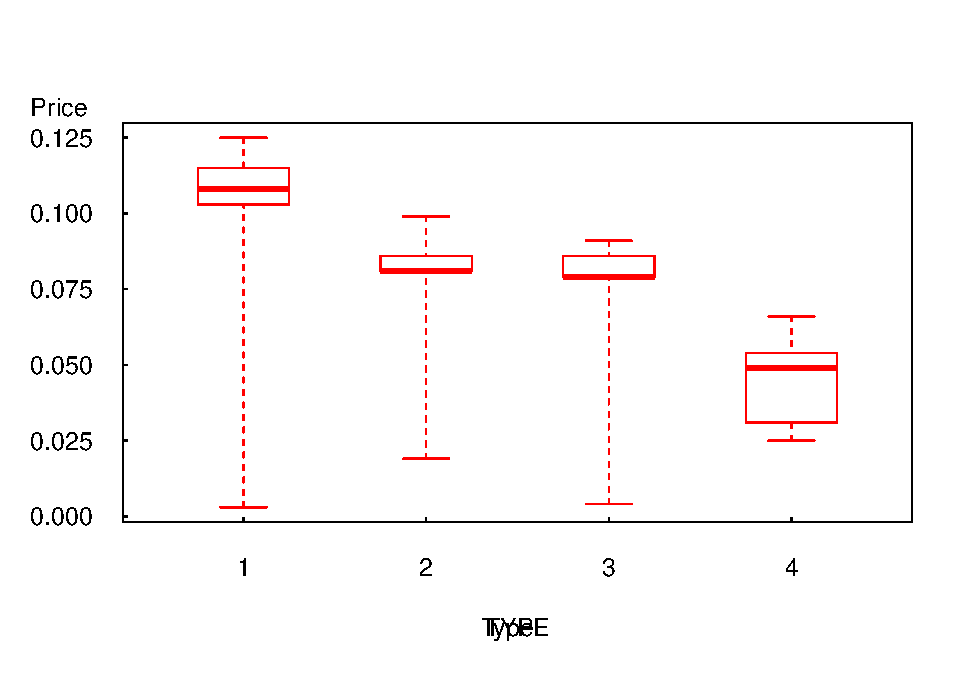
\includegraphics{LongPanelDataScripts_files/figure-latex/unnamed-chunk-102-1.pdf}

\hypertarget{note-the-small-relationships-among-prices}{%
\subsection{Note the small relationships among prices}\label{note-the-small-relationships-among-prices}}

\begin{Shaded}
\begin{Highlighting}[]
\KeywordTok{cor}\NormalTok{(yogurtdata[, }\KeywordTok{c}\NormalTok{(}\StringTok{"py"}\NormalTok{, }\StringTok{"pd"}\NormalTok{, }\StringTok{"pw"}\NormalTok{, }\StringTok{"ph"}\NormalTok{)])}
\end{Highlighting}
\end{Shaded}

\begin{verbatim}
            py          pd         pw          ph
py  1.00000000  0.03201738  0.1538099 -0.01844819
pd  0.03201738  1.00000000  0.2428201 -0.04349290
pw  0.15380986  0.24282008  1.0000000 -0.02755800
ph -0.01844819 -0.04349290 -0.0275580  1.00000000
\end{verbatim}

\begin{Shaded}
\begin{Highlighting}[]
\KeywordTok{plot}\NormalTok{(pw}\OperatorTok{~}\NormalTok{pd, }\DataTypeTok{data=}\NormalTok{yogurtdata, }\DataTypeTok{yaxt=}\StringTok{"n"}\NormalTok{, }\DataTypeTok{xaxt=}\StringTok{"n"}\NormalTok{, }\DataTypeTok{ylab=}\StringTok{""}\NormalTok{, }\DataTypeTok{xlab=}\StringTok{""}\NormalTok{)}
\KeywordTok{axis}\NormalTok{(}\DecValTok{2}\NormalTok{, }\DataTypeTok{at=}\KeywordTok{seq}\NormalTok{(}\FloatTok{0.00}\NormalTok{, }\FloatTok{0.20}\NormalTok{, }\DataTypeTok{by=}\FloatTok{0.01}\NormalTok{), }\DataTypeTok{las=}\DecValTok{1}\NormalTok{, }\DataTypeTok{font=}\DecValTok{10}\NormalTok{, }\DataTypeTok{cex=}\FloatTok{0.005}\NormalTok{, }\DataTypeTok{tck=}\FloatTok{0.01}\NormalTok{)}
\KeywordTok{axis}\NormalTok{(}\DecValTok{2}\NormalTok{, }\DataTypeTok{at=}\KeywordTok{seq}\NormalTok{(}\FloatTok{0.00}\NormalTok{, }\FloatTok{0.20}\NormalTok{, }\DataTypeTok{by=}\FloatTok{0.002}\NormalTok{),}\DataTypeTok{lab=}\NormalTok{F, }\DataTypeTok{tck=}\FloatTok{0.005}\NormalTok{)}
\KeywordTok{axis}\NormalTok{(}\DecValTok{1}\NormalTok{, }\DataTypeTok{at=}\KeywordTok{seq}\NormalTok{(}\FloatTok{0.01}\NormalTok{, }\FloatTok{0.12}\NormalTok{, }\DataTypeTok{by=}\FloatTok{0.01}\NormalTok{), }\DataTypeTok{font=}\DecValTok{10}\NormalTok{, }\DataTypeTok{cex=}\FloatTok{0.005}\NormalTok{, }\DataTypeTok{tck=}\FloatTok{0.01}\NormalTok{)}
\KeywordTok{axis}\NormalTok{(}\DecValTok{1}\NormalTok{, }\DataTypeTok{at=}\KeywordTok{seq}\NormalTok{(}\FloatTok{0.01}\NormalTok{, }\FloatTok{0.12}\NormalTok{, }\DataTypeTok{by=}\FloatTok{0.002}\NormalTok{), }\DataTypeTok{lab=}\NormalTok{F, }\DataTypeTok{tck=}\FloatTok{0.005}\NormalTok{)}
\KeywordTok{mtext}\NormalTok{(}\StringTok{"pw"}\NormalTok{, }\DataTypeTok{side=}\DecValTok{2}\NormalTok{, }\DataTypeTok{line=}\DecValTok{1}\NormalTok{, }\DataTypeTok{at=}\FloatTok{0.11}\NormalTok{, }\DataTypeTok{las=}\DecValTok{1}\NormalTok{, }\DataTypeTok{font=}\DecValTok{10}\NormalTok{)}
\KeywordTok{mtext}\NormalTok{(}\StringTok{"pd"}\NormalTok{, }\DataTypeTok{side=}\DecValTok{1}\NormalTok{, }\DataTypeTok{line=}\DecValTok{3}\NormalTok{, }\DataTypeTok{at=}\FloatTok{0.062}\NormalTok{, }\DataTypeTok{font=}\DecValTok{10}\NormalTok{)}
\end{Highlighting}
\end{Shaded}

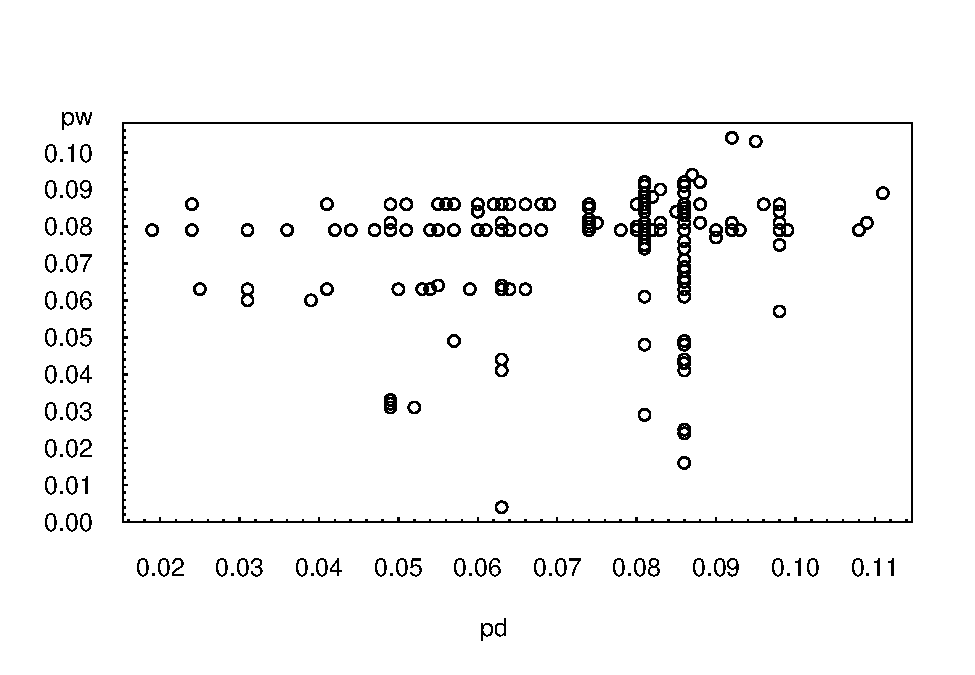
\includegraphics{LongPanelDataScripts_files/figure-latex/unnamed-chunk-103-1.pdf}

\hypertarget{more-on-prices}{%
\subsection{More on prices}\label{more-on-prices}}

\begin{Shaded}
\begin{Highlighting}[]
\KeywordTok{summary}\NormalTok{(yogurtdata}\OperatorTok{$}\NormalTok{PRICE)}
\end{Highlighting}
\end{Shaded}

\begin{verbatim}
   Min. 1st Qu.  Median    Mean 3rd Qu.    Max. 
0.00300 0.07900 0.08300 0.08495 0.10300 0.12500 
\end{verbatim}

\begin{Shaded}
\begin{Highlighting}[]
\KeywordTok{range}\NormalTok{(yogurtdata}\OperatorTok{$}\NormalTok{PRICE)}
\end{Highlighting}
\end{Shaded}

\begin{verbatim}
[1] 0.003 0.125
\end{verbatim}

\begin{Shaded}
\begin{Highlighting}[]
\KeywordTok{which}\NormalTok{(yogurtdata}\OperatorTok{$}\NormalTok{PRICE }\OperatorTok{==}\StringTok{ }\KeywordTok{min}\NormalTok{(yogurtdata}\OperatorTok{$}\NormalTok{PRICE))}
\end{Highlighting}
\end{Shaded}

\begin{verbatim}
[1] 1210 1215 1930 1931 2381
\end{verbatim}

\begin{Shaded}
\begin{Highlighting}[]
\KeywordTok{which}\NormalTok{(yogurtdata}\OperatorTok{$}\NormalTok{PRICE }\OperatorTok{==}\StringTok{ }\KeywordTok{max}\NormalTok{(yogurtdata}\OperatorTok{$}\NormalTok{PRICE))}
\end{Highlighting}
\end{Shaded}

\begin{verbatim}
[1]   71  952  961 1212 1213 1214 1929 2199
\end{verbatim}

\begin{Shaded}
\begin{Highlighting}[]
\KeywordTok{library}\NormalTok{(nnet)}
\NormalTok{test <-}\StringTok{ }\KeywordTok{multinom}\NormalTok{(TYPE }\OperatorTok{~}\StringTok{ }\NormalTok{FEATURE}\OperatorTok{+}\NormalTok{PRICE, }\DataTypeTok{data =}\NormalTok{ yogurtdata)}
\end{Highlighting}
\end{Shaded}

\begin{verbatim}
# weights:  16 (9 variable)
initial  value 3343.741999 
iter  10 value 2587.908201
iter  20 value 2364.679552
iter  30 value 2360.691887
final  value 2360.191855 
converged
\end{verbatim}

\begin{Shaded}
\begin{Highlighting}[]
\KeywordTok{summary}\NormalTok{(test)}
\end{Highlighting}
\end{Shaded}

\begin{verbatim}
Call:
multinom(formula = TYPE ~ FEATURE + PRICE, data = yogurtdata)

Coefficients:
  (Intercept)    FEATURE      PRICE
2    7.458657 -1.8039258  -80.44352
3    6.883787 -1.7072398  -80.32860
4    8.529886 -0.9595805 -139.53475

Std. Errors:
  (Intercept)   FEATURE    PRICE
2   0.3509758 0.2400558 3.836776
3   0.3756930 0.2673651 4.169266
4   0.4773418 0.3787246 6.632942

Residual Deviance: 4720.384 
AIC: 4738.384 
\end{verbatim}

\hypertarget{fitting-fixed-effects-multinomial-logit-model-by-the-poisson-log-linear-model}{%
\section{Fitting fixed effects multinomial logit model by the poisson log-linear model}\label{fitting-fixed-effects-multinomial-logit-model-by-the-poisson-log-linear-model}}

\begin{Shaded}
\begin{Highlighting}[]
\CommentTok{# RESHAPE yogurtdata FROM WIDE FORMAT INTO LONG FORMAT}
\NormalTok{yogurt<-}\KeywordTok{reshape}\NormalTok{(yogurtdata, }\DataTypeTok{varying=}\KeywordTok{list}\NormalTok{(}\KeywordTok{c}\NormalTok{(}\StringTok{"yoplait"}\NormalTok{,}\StringTok{"dannon"}\NormalTok{,}\StringTok{"weight"}\NormalTok{,}\StringTok{"hiland"}\NormalTok{)), }\DataTypeTok{v.names=}
\StringTok{"choice"}\NormalTok{, }\DataTypeTok{idvar=}\StringTok{"occasion"}\NormalTok{,}\DataTypeTok{timevar=}\StringTok{"brand"}\NormalTok{, }\DataTypeTok{direction=}\StringTok{"long"}\NormalTok{) }
\NormalTok{yogurt<-yogurt[}\KeywordTok{order}\NormalTok{(yogurt}\OperatorTok{$}\NormalTok{occasion),]}
\NormalTok{yogurt[}\DecValTok{1}\OperatorTok{:}\DecValTok{8}\NormalTok{,]}
\end{Highlighting}
\end{Shaded}

\begin{verbatim}
    id fy fd fw fh    py    pd    pw    ph occasion TYPE PRICE FEATURE
1.1  1  0  0  0  0 0.108 0.081 0.079 0.061        1    3 0.079       0
1.2  1  0  0  0  0 0.108 0.081 0.079 0.061        1    3 0.079       0
1.3  1  0  0  0  0 0.108 0.081 0.079 0.061        1    3 0.079       0
1.4  1  0  0  0  0 0.108 0.081 0.079 0.061        1    3 0.079       0
2.1  1  0  0  0  0 0.108 0.098 0.075 0.064        2    2 0.098       0
2.2  1  0  0  0  0 0.108 0.098 0.075 0.064        2    2 0.098       0
2.3  1  0  0  0  0 0.108 0.098 0.075 0.064        2    2 0.098       0
2.4  1  0  0  0  0 0.108 0.098 0.075 0.064        2    2 0.098       0
    brand choice
1.1     1      0
1.2     2      0
1.3     3      1
1.4     4      0
2.1     1      0
2.2     2      1
2.3     3      0
2.4     4      0
\end{verbatim}

\begin{Shaded}
\begin{Highlighting}[]
\NormalTok{yogurt}\OperatorTok{$}\NormalTok{brand<-}\KeywordTok{factor}\NormalTok{(yogurt}\OperatorTok{$}\NormalTok{brand)}
\NormalTok{yogurt}\OperatorTok{$}\NormalTok{occasion<-}\KeywordTok{factor}\NormalTok{(yogurt}\OperatorTok{$}\NormalTok{occasion)}
\CommentTok{# yogurtloglinear<-glm(choice~brand+occasion+FEATURE+PRICE-1, data=yogurt, family=# poisson(link="log"))}
\CommentTok{# THE ABOVE GLM INCLUDES THE FIXED EFFECTS OF THE 2412 OCCASIONS, WHICH ARE}
\CommentTok{# NUISANCE PARAMETERS, THE ESTIMATES ARE NOT OBTAINED SIMPLY BECAUSE THE }
\CommentTok{# LARGE NUMBER. }
\CommentTok{# GLM USE ITERATIVELY REWEIGHTED LEAST SQUARES TO ESTIMATE, COMPARED WITH }
\CommentTok{# GENMOD IN SAS # USING MAXIMUMLIKELIHOOD.}
\CommentTok{# DROP occasion THE GLM IS ESTIMATABLE}
\NormalTok{model1 <-}\StringTok{ }\KeywordTok{glm}\NormalTok{(choice}\OperatorTok{~}\NormalTok{brand}\OperatorTok{+}\NormalTok{FEATURE}\OperatorTok{+}\NormalTok{PRICE}\DecValTok{-1}\NormalTok{, }\DataTypeTok{data=}\NormalTok{yogurt, }\DataTypeTok{family=}\KeywordTok{poisson}\NormalTok{(}\DataTypeTok{link=}\StringTok{"log"}\NormalTok{))}
\KeywordTok{summary}\NormalTok{(model1)}
\end{Highlighting}
\end{Shaded}

\begin{verbatim}

Call:
glm(formula = choice ~ brand + FEATURE + PRICE - 1, family = poisson(link = "log"), 
    data = yogurt)

Deviance Residuals: 
     Min        1Q    Median        3Q       Max  
-0.89683  -0.82357  -0.67716   0.01585   2.26052  

Coefficients:
          Estimate Std. Error z value Pr(>|z|)    
brand1  -1.081e+00  9.183e-02  -11.78   <2e-16 ***
brand2  -9.109e-01  9.079e-02  -10.03   <2e-16 ***
brand3  -1.473e+00  9.497e-02  -15.51   <2e-16 ***
brand4  -3.526e+00  1.459e-01  -24.16   <2e-16 ***
FEATURE  3.206e-16  8.028e-02    0.00        1    
PRICE   -1.375e-13  9.840e-01    0.00        1    
---
Signif. codes:  0 '***' 0.001 '**' 0.01 '*' 0.05 '.' 0.1 ' ' 1

(Dispersion parameter for poisson family taken to be 1)

    Null deviance: 14472.0  on 9648  degrees of freedom
Residual deviance:  5665.9  on 9642  degrees of freedom
AIC: 10502

Number of Fisher Scoring iterations: 6
\end{verbatim}

\hypertarget{fitting-multinomial-logit-model-with-random-intercepts-by-the-possion-log-linear-with-random-intercepts}{%
\section{Fitting multinomial logit model with random intercepts by the possion-log-linear with random intercepts}\label{fitting-multinomial-logit-model-with-random-intercepts-by-the-possion-log-linear-with-random-intercepts}}

\begin{Shaded}
\begin{Highlighting}[]
\KeywordTok{library}\NormalTok{(MASS)}
\CommentTok{# glmmPQL(choice~feature+price+occasion, data=yogurt, family=poisson(link="log"), random=~1|brand)}
\CommentTok{# THE ABOVE HAS SIMILAR PROBLEM WHEN INCLUDING occasion AS FIXED EFFECTS}
\CommentTok{# OTHERWISE IT IS ESTIMATABLE IN R; HOWEVER THE RESULT IS QUITE DIFFERENT FROM # THAT OF SAS}
\KeywordTok{glmmPQL}\NormalTok{(choice}\OperatorTok{~}\NormalTok{FEATURE}\OperatorTok{+}\NormalTok{PRICE, }\DataTypeTok{data=}\NormalTok{yogurt, }\DataTypeTok{family=}\KeywordTok{poisson}\NormalTok{(}\DataTypeTok{link=}\StringTok{"log"}\NormalTok{), }\DataTypeTok{random=}\OperatorTok{~}\DecValTok{1}\OperatorTok{|}\NormalTok{brand)}
\end{Highlighting}
\end{Shaded}

\begin{verbatim}
iteration 1
\end{verbatim}

\begin{verbatim}
iteration 2
\end{verbatim}

\begin{verbatim}
iteration 3
\end{verbatim}

\begin{verbatim}
iteration 4
\end{verbatim}

\begin{verbatim}
iteration 5
\end{verbatim}

\begin{verbatim}
iteration 6
\end{verbatim}

\begin{verbatim}
Linear mixed-effects model fit by maximum likelihood
  Data: yogurt 
  Log-likelihood: NA
  Fixed: choice ~ FEATURE + PRICE 
  (Intercept)       FEATURE         PRICE 
-1.743787e+00  2.005532e-14  2.982266e-13 

Random effects:
 Formula: ~1 | brand
        (Intercept)  Residual
StdDev:    1.040625 0.8639861

Variance function:
 Structure: fixed weights
 Formula: ~invwt 
Number of Observations: 9648
Number of Groups: 4 
\end{verbatim}

\bibliography{Bibliography/LDAReferenceC.bib}


\end{document}
